% !TEX encoding = UTF-8 Unicode
%%
%% This is file `thesis-ex.tex',
%% generated with the docstrip utility.
%%
%% The original source files were:
%%
%% uiucthesis2009.dtx  (with options: `example')
%% 

%\newcommand*{\ATLASLATEXPATH}{latex/}


\documentclass[fullpage, hidelinks]{uiucthesis2009}

%\RequirePackage{lineno}
%\linenumbers

\usepackage{graphicx}
\usepackage{placeins}
\usepackage{amsmath}
\usepackage{amssymb}
\usepackage{graphicx}
\usepackage{pdfpages}
\usepackage{amsmath}
\usepackage{slashed}
\usepackage{placeins}
\usepackage{tabularx}
\usepackage{booktabs}
\usepackage{subcaption}
%\usepackage{sectsty}
%\chapterfont{\centering}
\usepackage[pagestyles]{titlesec}
\usepackage{epigraph} 
 
 
\titleformat{\chapter}[display]
   {\normalfont\huge\bfseries\centering}{\centering\chaptertitlename\ \thechapter}{20pt}{\Huge}
\titlespacing*{\chapter}
   {0pt}{50pt}{40pt}


\usepackage[
    backend=bibtex,
    url=false,
    doi=false,
    maxbibnames=1,
    hyperref=true,
    backref=true,
    style=numeric-comp,
    sorting=none,
    giveninits=true,
]{biblatex}


%remove "in" in references
\renewbibmacro{in:}{}

%make journal name the hyperlink
\DeclareFieldFormat{string+doi}{%
\iffieldundef{doi}{#1}{\href{http://dx.doi.org/\thefield{doi}}{#1}}}
\renewbibmacro*{journal+issuetitle}{%
%\usebibmacro{string+doi}{%
\printtext[string+doi]{%
\usebibmacro{journal}%
\setunit*{\addspace}%
\iffieldundef{series}
{}
{\newunit
\printfield{series}%
\setunit{\addspace}}%
\usebibmacro{volume+number+eid}%
\setunit{\addspace}%
\usebibmacro{issue+date}%
\setunit{\addcolon\space}%
\usebibmacro{issue}%
\setunit{\bibpagespunct}%
\printfield{pages}%
\newunit
}}
    \renewbibmacro*{note+pages}{%
      \printfield{note}%
      \newunit}

\DefineBibliographyStrings{english}{%
page = {},
pages = {}
}


\DeclareFieldFormat[article]{title}{\textit{#1}\isdot}
\DeclareFieldFormat[booklet]{title}{\textit{#1}\isdot}
\DeclareFieldFormat[report]{title}{\textit{#1}\isdot}
\DeclareFieldFormat[misc]{title}{\textit{#1}\isdot}
\DeclareFieldFormat[article]{journaltitle}{#1\isdot}
\DeclareFieldFormat[article]{journalsubtitle}{#1\isdot}
\DeclareFieldFormat[article]{volume}{\textbf{#1}\isdot}
\DeclareFieldFormat{pages}{\mkfirstpage[{\mkpageprefix[bookpagination]}]{#1}}

% Suppress issue number
\AtEveryBibitem{
\ifentrytype{article}{\clearfield{number}}{}
\ifentrytype{article}{\clearfield{issn}}{}}

\usepackage{hyperref}
\hypersetup{
     colorlinks = true,
     linkcolor = magenta, 
     citecolor = blue,
     urlcolor = red,}

%     linkcolor = red: contents, figure refs, section refs, cited on page__
%     citecolor = blue: citations [ ] ,
%     urlcolor = cyan: hyperlinks in citations



% !TEX encoding = UTF-8 Unicode
% !TEX root = thesis-ex.tex
\newcommand{\sigmainel}{\sigma_{\mathrm{inel}}^{\mathrm{NN}}}
\newcommand{\DeltaP}{$\Delta_P(\rvar)$}
\newcommand{\DeltaTheta}{$\Delta_{\Theta(\rvar)}$}
\newcommand{\RP}{$R_{P(\rvar)}$}
\newcommand{\RTheta}{$R_{\Theta(\rvar)}$}
\newcommand{\DeltaDptr}{\mbox{$\Delta\Dptr$}}
\newcommand{\alphas}{$\alpha_s$}

\newcommand{\EM}{\mbox{\text{EM}}}
\newcommand{\HI}{\mbox{\text{HI}}}

\newcommand{\ptEM}{\mbox{$p_{\mathrm{T}}^{\mathrm{EM}}$}}
\newcommand{\ptHI}{\mbox{$p_{\mathrm{T}}^{\mathrm{HI}}$}}
\newcommand{\REM}{\mbox{$R_{\mathrm{EM}}$}}
\newcommand{\RHI}{\mbox{$R_{\mathrm{HI}}$}}
\newcommand{\sEM}{\mbox{$s_{\mathrm{EM}}$}}
\newcommand{\sHI}{\mbox{$s_{\mathrm{HI}}$}}
\newcommand{\deltaEM}{\mbox{$\Delta_{\mathrm{EM}}$}}
\newcommand{\deltaHI}{\mbox{$\Delta_{\mathrm{HI}}$}}




\newcommand{\pttrkreco}{\mbox{$p_{{\mathrm{T}}}^{\mathrm{trk,reco}}$}}
\newcommand{\Dptrmeas}{\mbox{$D^{\mathrm{meas}}(\pT,r)$}}
\newcommand{\Dptrsub}{\mbox{$D^{\mathrm{sub}}(\pT,r)$}}
\newcommand{\Rdptr}{\mbox{$R_{D( \pT, r)}$}}


\newcommand{\phijet}{\mbox{$\phi^{\mathrm{jet}}$}}
\newcommand{\NchUECone}{\mbox{$N_{\mathrm{ch}}^{\mathrm{UE\ cone}}$}}


\newcommand{\radlen}{\mbox{$X_{0}$}}
\newcommand{\intlen}{\mbox{$\lambda_{I}$}}
\newcommand{\rphi}{\mbox{$R - \phi$}}


\newcommand\blfootnote[1]{%
  \begingroup
  \renewcommand\thefootnote{}\footnote{#1}%
  \addtocounter{footnote}{-1}%
  \endgroup
}


\newcommand{\AtlasCopyrightFooter}{%
  \parbox[b]{\linewidth}{%
    \rmfamily\mdseries\fontsize{10}{12}\selectfont
    \copyright\ 2018 \ CERN for the benefit of the ATLAS Collaboration.\newline
    Reproduction of this article or parts of it is allowed as specified in the CC-BY-4.0 license.
  }\par
}

\newcommand{\pb}{pb$^{-1}$}
\newcommand{\nb}{nb$^{-1}$}

\newcommand{\pttrktruth}{\mbox{$p_{\mathrm{T}}^{\mathrm{trk, Truth}}$}}
\newcommand{\etatrktruth}{\mbox{$\eta^{\mathrm{trk}}_{\mathrm{truth}}$}}


\newcommand{\Dptr}{\mbox{$D( \pT, r)$}}
\newcommand{\RDptr}{\mbox{$R_{D( p_{\mathrm{T}}, r)}$}}
\newcommand{\nucnuc}{\mbox{A+A}}
\newcommand{\AuAu}{\mbox{Au+Au}}
\newcommand{\PbPb}{\mbox{Pb+Pb}}
\newcommand{\pbpb}{\mbox{Pb+Pb}}
\newcommand{\pp}{\mbox{$pp$}}
\newcommand{\dR}{\mbox{$\Delta R$}}

\newcommand{\pTmin}{\mbox{$p_{\mathrm{T,min}}$}}
\newcommand{\pTmax}{\mbox{$p_{\mathrm{T,max}}$}}
\newcommand{\dpT}{\mbox{$\mathrm{d}p_{\mathrm{T}}$}}
\newcommand{\NBJ}{\mbox{$R_{\Delta R}$}}
\newcommand{\Etmiss}{\mbox{$E_{\mathrm{T}^{\mathrm{miss}}}$}}
\newcommand{\Et}{\mbox{$E_{\mathrm{T}}$}}
\newcommand{\pt}{\mbox{$p_{\mathrm{T}}$}}
\newcommand{\pT}{\mbox{$p_{\mathrm{T}}$}}
\newcommand{\RNBJ}{\mbox{$\rho_{R_{\Delta R}}$}}
\newcommand{\ETtest}{\mbox{$E_{\mathrm{T}}^\mathrm{test}$}}
\newcommand{\ETnbj}{\mbox{$E_{\mathrm{T}}^\mathrm{nbr}$}}
\newcommand{\ETcombi}{\mbox{$E_{\mathrm{T}}^\mathrm{comb}$}}
\newcommand{\ETmerged}{\mbox{$E_{\mathrm{T}}^\mathrm{merged}$}}

\newcommand{\ANpart}{\mbox{$\langle N_{\mathrm{part}}\rangle$}}
\newcommand{\Ncoll}{\mbox{$N_{\mathrm{coll}}$}}
%\newcommand{\Nevt}{\mbox{$N_{\mathrm{evt}}$}}
\newcommand{\Ncone}{\mbox{$N_{\mathrm{cone}}$}}
\newcommand{\Njetcent}{\mbox{$N_{\mathrm{jet}}^{\mathrm{cent}}$}}
\newcommand{\Njet}{\mbox{$N_{\mathrm{jet}}$}}
\newcommand{\Nch}{\mbox{$N_{\mathrm{ch}}$}}
\newcommand{\NchUE}{\mbox{$N_{\mathrm{ch}}^{\mathrm{UE}}$}}
\newcommand{\nchUE}{\mbox{$n_{\mathrm{ch}}^{\mathrm{UE}}$}}
\newcommand{\nchmeas}{\mbox{$n_{\mathrm{ch}}^{\mathrm{meas}}$}}
\newcommand{\nchsub}{\mbox{$n_{\mathrm{ch}}^{\mathrm{sub}}$}}
\newcommand{\nchunf}{\mbox{$n_{\mathrm{ch}}^{\mathrm{unfolded}}$}}
\newcommand{\nch}{\mbox{$n_{\mathrm{ch}}$}}
\newcommand{\Npart}{\mbox{$N_{\mathrm{part}}$}}
\newcommand{\Ntptrt}{N_{\mathrm{2p}}}
\newcommand{\Ntptr}{\mbox{$N_{\mathrm{2p}}$}}
\newcommand{\Nraw}{\mbox{$N^{\mathrm{raw}}$}}
\newcommand{\sqrtsnn}{\mbox{$\sqrt{s_{_\text{NN}}}$}}
%\newcommand*{\sqn}{\ensuremath{\sqrt{s_{_\text{NN}}}}\xspace}
\newcommand{\sqrts}{\mbox{$\sqrt{s}$}}
\newcommand{\centrm}{\mathrm{cent}}
\newcommand{\pythia}{{\textsc PYTHIA}}
\newcommand{\pythiasix}{{\textsc Pythia}6}
\newcommand{\pythiaeight}{\textsc{Pythia}8}
\newcommand{\herwig}{{\textsc Herwig++}}
\newcommand{\powheg}{\textsc{Powheg}}
%\newcommand{\text}{\textit{}}


\newcommand{\RAA}{\mbox{$R_{\rm AA}$}}
\newcommand{\RFive}{\mbox{$R = 0.5$}}
\newcommand{\RFour}{\mbox{$R = 0.4$}}
\newcommand{\RThree}{\mbox{$R = 0.3$}}
\newcommand{\RTwo}{\mbox{$R= 0.2$}}
\newcommand{\Rcp}{\mbox{$R_{\rm CP}$}}
\newcommand{\Rpc}{\mbox{$R_{\rm PC}$}}
\newcommand{\Sk}{\mbox{$S(k)$}}
\newcommand{\TAA}{\mbox{$T_{\mathrm{AA}}$}}

\newcommand{\antikt}{\mbox{anti-\kt}}
\newcommand{\avgpttrue}{\mbox{$\langle p_{\mathrm{T}}^{\mathrm{truth}}\rangle$}}
\newcommand{\centup}{^{\mathrm{cent}}}
\newcommand{\deffrel}{\mbox{$\delta \varepsilon/\varepsilon$}}
\newcommand{\ETfcal}{\mbox{$\Sigma E_{\mathrm{T}}^{\mathrm{FCal}}$}}
\newcommand{\eff}{\mbox{$\varepsilon$}}
\newcommand{\ETtruth}{\mbox{$E_{\mathrm{T}}^{\mathrm{truth}}$}}
\newcommand{\fs}{\mbox{${f_{\mathrm{S}}}$}}
\newcommand{\gjet}{\mbox{$\gamma$-jet}}
\newcommand{\invnb}{\mbox{${\rm nb^{-1}}$}}
\newcommand{\kt}{\mbox{$k_{t}$}}
\newcommand{\sumet}{\mbox{$\Sigma E_{\mathrm{T}}$}}
\newcommand{\ETrec}{\mbox{$E_{\mathrm{T}}^{\mathrm{rec}}$}}
\newcommand{\ETtbyf}{\mbox{$E_{\mathrm{T}}^{3\times 4}$}}
\newcommand{\ETsbys}{\mbox{$E_{\mathrm{T}}^{7\times 7}$}}
\newcommand{\Dphi}{\mbox{$\Delta \phi$}}
\newcommand{\Deta}{\mbox{$\Delta \eta$}}
\newcommand{\DpT}{\mbox{$\Delta \pT$}}
\newcommand{\Dz}{\mbox{$D(z)$}}
\newcommand{\Dzmeas}{\mbox{$D^{\mathrm{meas}}(z)$}}
\newcommand{\Dzsub}{\mbox{$D^{\mathrm{sub}}(z)$}}
\newcommand{\Dpt}{\mbox{$D(\pT)$}}
\newcommand{\Dptmeas}{\mbox{$D^{\mathrm{meas}}(\pT)$}}
\newcommand{\Dptsub}{\mbox{$D^{\mathrm{sub}}(\pttrk)$}}
\newcommand{\Dptratio}{\mbox{$D(\pT)|_{\mathrm{cent}}/D(\pT)|_{\mathrm{60-80}}$}}
\newcommand{\Dzratio}{\mbox{$D(z)|_{\mathrm{cent}}/D(z)|_{\mathrm{60-80}}$}}
\newcommand{\Delpt}{\mbox{$\Delta \pT$}}
\newcommand{\DRtrk}{\mbox{$\Delta R_{\mathrm{trk}}$}}
\newcommand{\effpteta}{\mbox{$\varepsilon(\pT, \eta)$}}
\newcommand{\effpt}{\mbox{$\varepsilon(\pT)$}}
\newcommand{\phat}{\mbox{$\hat{p}_{\mathrm{T}}$}}
\newcommand{\pthatmin}{\mbox{$\hat{p}^{\mathrm{min}}_{\mathrm{T}}$}}
\newcommand{\pthat}{\mbox{$\hat{p}_{\mathrm{T}}$}}
\newcommand{\etajet}{\mbox{$\eta^{\mathrm{jet}}$}}
\newcommand{\pTjet}{\mbox{$p_{{\mathrm{T}}}$}}
\newcommand{\pTjetcorr}{\mbox{$p_{{\mathrm{T}}}^{\mathrm{corr}}$}}
\newcommand{\pTch}{\mbox{$p_{{\mathrm{T}}}^{\mathrm{ch}}$}}
\newcommand{\pTtrk}{\mbox{$p_{{\mathrm{T}}}^{\mathrm{ch}}$}}
\newcommand{\pttrk}{\mbox{$p_{\mathrm{T}}^{\mathrm{ch}}$}}
%\newcommand{\pttrk}{\mbox{$p_{\mathrm{T}}^{\mathrm{trk}}$}}
%\newcommand{\pTtrk}{\mbox{$p_{{\mathrm{T}}}^{\mathrm{trk}}$}}
\newcommand{\pTrec}{\mbox{$p_{{\mathrm{T}}}^{\mathrm{rec}}$}}
\newcommand{\pTtrue}{\mbox{$p_{\mathrm{T}}^{\mathrm{truth}}$}}
\newcommand{\etatrue}{\mbox{$\eta^{\mathrm{truth}}$}}
\newcommand{\ztrue}{\mbox{$z^{\mathrm{truth}}$}}
\newcommand{\zrec}{\mbox{$z^{\mathrm{rec}}$}}
\newcommand{\ptvjet}{\mbox{$\displaystyle {\vec{p}_{\mathrm{T}}}^{\, \mathrm{jet}}$}}
\newcommand{\ptvchg}{\mbox{$\displaystyle {\vec{p}_{\mathrm{T}}}^{\, \mathrm{chg}}$}}
\newcommand{\ntrue}{\mbox{$N^{\mathrm{truth}}$}}
\newcommand{\nmatch}{\mbox{$N^{\mathrm{match}}$}}
\newcommand{\rcpcorr}{\mbox{$R_{\mathrm{CP}}$}}
\newcommand{\rcpraw}{\mbox{$R_{\mathrm{CP}}^{\mathrm{meas}}$}}
\newcommand{\unfdn}{_{\mathrm{unf}}}
\newcommand{\xini}{\mbox{$x_{\mathrm{ini}}$}}
\newcommand{\vtjet}{\mbox{$v_2^{\mathrm{jet}}$}}
\newcommand{\vtjetmeas}{\mbox{${v_2^{\mathrm{jet}}|_{\mathrm{meas}}}$}}
\newcommand{\vtwo}{\mbox{$v_2$}}
\newcommand{\Rdz}{\mbox{$R_{D(z)}$}}
\newcommand{\Rdpt}{\mbox{$R_{D(\pT)}$}}
\newcommand{\Rdzsub}{\mbox{$R_{D(z)}^{\mathrm{sub}}$}}
\newcommand{\Rdptsub}{\mbox{$R_{D(\pT)}^{\mathrm{sub}}$}}
\newcommand{\Psit}{\mbox{$\Psi_2$}}

\newcommand{\Psires}{\mbox{$\mathrm{Res}\{\Psi_2\}$}}
\newcommand{\Rpsi}{\mbox{$R_{\Delta \phi}$}}
\newcommand{\diff}{\mathrm{d}}
\newcommand{\dpsi}{\mbox{$\Delta\phi$}}
\newcommand{\dNdpTdpsi}{\mbox{$\diff^2\Njet/\diff\pt\diff\dpsi$}}
\newcommand{\dNdpTdpsiRaw}{\mbox{$\dfrac{\diff^2N_{\mathrm{jet}}^{\mathrm{raw}}}{\diff\pt\diff\dpsi}$}}
\newcommand{\dNdpTdpsiCorr}{\mbox{$\dfrac{\diff^2N_{\mathrm{jet}}^{\mathrm{corr}}}{\diff\pt\diff\dpsi}$}}

\newcommand{\ETjet}{\mbox{$\ET^{\mathrm{jet}}$}}
\newcommand{\pbarp}{\mbox{$p+\bar{p}$}}
\newcommand{\pPb}{\mbox{$p$+Pb}}
%\newcommand{\pt}{\mbox{$p_T$}}
\newcommand{\ptjet}{\mbox{$p_{\mathrm{T}}^{\mathrm{jet}}$}}
%\newcommand{\pt}{\mbox{$p_{\mathrm{T}}$}}
%\newcommand{\etatrk}{\mbox{$\eta^{\mathrm{trk}}$}}
\newcommand{\etatrk}{\mbox{$\eta^{\mathrm{ch}}$}}
\newcommand{\ptpart}{\mbox{$p_{\mathrm{T}}^{\mathrm{part}}$}}
\newcommand{\pttruth}{\mbox{$p_{\mathrm{T}}^{\mathrm{reco}}$}}
\newcommand{\ptreco}{\mbox{$p_{\mathrm{T}}^{\mathrm{truth}}$}}
%\newcommand{\etapart}{\mbox{$\eta^{part}$}}
\newcommand{\ystar}{\mbox{$y^{*}_{\mathrm{jet}}$}}
\newcommand{\yjet}{\mbox{$y^{\mathrm{jet}}$}}
\newcommand{\Lres}{\mbox{$L_{\mathrm{res}}$}}
\newcommand{\Rres}{\mbox{$R_{\mathrm{res}}$}}
\newcommand{\dndeta}{\mbox{$1/\Nevt \, d\Nch/d\eta$}}
\newcommand{\RpPb}{\mbox{$R_{p\mathrm{Pb}}$}}
\newcommand{\Jt}{\mbox{$j_{\mathrm{T}}$}}
\newcommand{\jt}{\mbox{$j_{\mathrm{T}}$}}
\newcommand{\xt}{\mbox{$x_{\mathrm{T}}$}}
\newcommand{\ETtrue}{\mbox{$E_{\mathrm{T}}^{\mathrm{truth}}$}}
\newcommand{\ETreco}{\mbox{$E_{\mathrm{T}}^{\mathrm{reco}}$}}
\newcommand{\RSix}{\mbox{$R= 0.6$}}
\newcommand{\EffJet}{\mbox{$\varepsilon_{\mathrm{jet}}$}}
\newcommand{\Aj}{\mbox{$A_{\mathrm{J}}$}}
\newcommand{\dphi}{$\Delta \phi$}
\newcommand{\p}{\partial}
\newcommand{\rvar}{\mbox{$r$}}
\renewcommand{\_}{{\tt \char`\_}}  % works properly only in \tt mode (!)
\newcommand{\z}{\mbox{$z$}}
\newcommand{\zunfolded}{\mbox{$z_{\mathrm{unfolded}}$}}
\newcommand{\zreco}{\mbox{$z_{\mathrm{reco}}$}}
\newcommand{\ztruth}{\mbox{$z_{\mathrm{truth}}$}}
\newcommand{\Rdzmeas}{\mbox{$R_{D(z)}^{\mathrm{meas}}$}}
\newcommand{\Rdptmeas}{\mbox{$R_{D(\pT)}^{\mathrm{meas}}$}}
\newcommand{\ptjettruth}{\mbox{$p_{{\mathrm{T}}}^{\mathrm{jet,truth}}$}}
\newcommand{\ptjetreco}{\mbox{$p_{{\mathrm{T}}}^{\mathrm{jet,reco}}$}}
\newcommand{\ptjetunfolded}{\mbox{$p_{{\mathrm{T}}}^{\mathrm{jet,unfolded}}$}}
\newcommand{\fd}{\mathrm{d}}
\newcommand{\cnchUE}{\mbox{$\tilde{n}_{\mathrm{ch}}^{\mathrm{UE+fake}}$}}

%\newcommand{\Dzunf}{\mbox{$D^{\mathrm{unfolded}}(z)$}}
%\newcommand{\Dptunf}{\mbox{$D^{\mathrm{unfolded}}(\pT)$}}
\newcommand{\Dzunf}{\mbox{$\frac{\diff\Nch}{\diff z}$}}
\newcommand{\Dptunf}{\mbox{$\frac{\diff\Nch}{\diff \pt}$}}

\newcommand{\GeV}{\mbox{GeV}}
\newcommand{\TeV}{\mbox{TeV}}
\newcommand{\dsigma}{\mbox{$\delta \sigma$}}
\newcommand{\hi}{\mathrm{HI}}
\newcommand{\emt}{\text{EMTopo}}
\newcommand{\tru}{\mathrm{Truth}}
\newcommand{\insitu}{\textit{in situ}}




\graphicspath{{logos/}{figures/}}
\addbibresource{thesis-ex.bib}

%TOC depth
%\setcounter{tocdepth}{0}




\begin{document}


\title{Measurement of angular and momentum distributions of charged particles within and around jets in P\MakeLowercase{b}+P\MakeLowercase{b} and \MakeLowercase{$pp$} collisions at $\sqrt{s_{\mathrm{NN}}}=$~5.02~T\MakeLowercase{e}V with ATLAS at the LHC}
\author{Akshat Puri}
\department{Physics}
\schools{B.Sc., State University of New York At Stony Brook, 2014}
\phdthesis
\advisor{Anne Marie Sickles}
\degreeyear{2019}
\committee{Professor Matthias Grosse Perdekamp, Chair\\Assistant Professor Anne Marie Sickles, Director of Research\\Professor Lance Cooper\\Assistant Professor Bryce Gadway}
\maketitle

\frontmatter

%% Create an abstract that can also be used for the ProQuest abstract.
%% Note that ProQuest truncates their abstracts at 350 words.
\setcounter{page}{2}
\renewcommand\abstractname{\textsc{ABSTRACT}}
\begin{abstract}

Heavy ion collision experiments have been centered around studying the extreme state of matter formed in such collisions, the quark-gluon plasma.
There have been efforts to measure and characterize this state of matter for almost two decades, first at the Relativistic Heavy Ion Collider and subsequently at the Large Hadron Collider.
While there have been different approaches to study it, correlated particle showers called jets have found a special place as a probe of the QGP.
Arising from highly energetic collisions between partons, jets are formed early enough in heavy ion collisions that they experience the formation of the QGP and its evolution.
They are modified from what they would be in a vacuum, and studying these modifications can give insight into the properties of the QGP as well as the strong interaction.

Jet measurements can focus on a variety of observables like yields, momenta, or fragmentation patterns, each with its own limitations and advantages.
This thesis presents a measurement of the angular distribution of charged particles around the jet axis as measured by the ATLAS detector for \pbpb\ and \pp\ collisions with a center of mass energy of $\sqrt{s_{\mathrm{NN}}}=$~5.02~TeV.
Comparing the measurement in the two  systems shows that charged particles carrying a transverse momenta \pt\ of less than 4 GeV have a broader distribution in \pbpb\ collisions, while those with $\pt > 4$ GeV have a narrower distribution.
Furthermore, there is an enhancement for particles with $\pt < 4$ GeV in \pbpb\ collisions, with the enhancement increasing up to 2 for \mbox{$\rvar < 0.3$} from the jet axis, and remaining constant for \mbox{$0.3 < \rvar < 0.6$}.
Charged particles with $\pt\ > 4$ \GeV\ show a small enhancement in the jet core for $\rvar < 0.05$, and are increasingly suppressed up to 0.5 for \mbox{$\rvar < 0.3$}.
This depletion remains constant for \mbox{$0.3 < \rvar < 0.6$}.

\end{abstract}

% Create a dedication in italics with no heading, centered vertically
% on the page.

\begin{dedication}
For my Mother, Father, and Brother
\end{dedication}

% Create an Acknowledgements page, many departments require you to
% include funding support in this.
% \chapter*{Acknowledgments}

% The thesis format requires the Table of Contents to come
% before any other major sections, all of these sections after
% the Table of Contents must be listed therein (i.e., use \chapter,
% not \chapter*).Common sections to have between the Table of
% Contents and the main text are:
%
% List of Tables
% List of Figures
% List Symbols and/or Abbreviations
% etc.


\chapter*{Acknowledgments}
% !TEX encoding = UTF-8 Unicode
% !TEX root = thesis-ex.tex

I would like to thank my advisors Professor Matthias Grosse Perdekamp and Anne Marie Sickles for their invaluable support and guidance throughout my time at the University of Illinois. Their experience as researchers was extremely valuable for myself and the rest of the group with whom I worked. I started working with Matthias as soon as I arrived in Illinois in 2013. I always appreciated his support, enthusiasm, and knowledge of physics. Besides his tremendous knowledge of nuclear and particle physics, Matthias is someone with whom one can discuss virtually anything; from politics to soccer. Anne was the driving force behind the ATLAS Heavy Ion group at Illinois. Thanks to her, it has grown into a strong group that contributes to the field in many different ways. It was a great experience to work for Matthias and Anne, and I thank them for providing me with the opportunity.

Martin Rybar, who was the postdoctoral researcher in our group for the majority of  the time I spent working on the ATLAS experiment has been a great advisor and friend. He was always keen to share his knowledge of physics and analysis with me, was there to help whenever I needed it, and taught me a lot of what I know about ATLAS. I definitely progressed much faster in my research thanks to him, and I am very happy for anyone who will get the great opportunity to work with him in the future. 

Next, I would like to thank all the members of the ATLAS collaboration for their expertise and for being great colleagues. It was a unique experience being part of such a team, and I am glad to say I got to do so. ATLAS is a large collaboration, and while I would like to thank everyone individually, I specifically want to mention my colleagues from the Heavy Ion group, with whom I worked closely. Thank you Peter Steinburg, Martin Spousta, Aaron Angerami, Brian Cole, Dennis Perepelitsa, Sebastian Tapia for providing insightful physics advice, reading my paper drafts, and for making the Heavy Ion group what it is. 

Lastly, want to thank my parents for all their support from the first day I can remember it. I cannot thank them enough for everything they have done. I am very happy they were able to attend my thesis defense, it meant a great deal to me, and I know it meant even more to them. My father, himself a physicist, always was eager to talk to me about my work. We had many interesting conversations in person and over the phone, and he always gave me interesting advice and ideas. My mother was always curious about what I was doing, about CERN, and in general about life as a graduate student. Thank you Daniel, Anton, and Michael for being great brothers and friends. I will be waiting for the days when you will be defending, and I hope things keep going smoothly for you. While she could not be with us now, my late grandmother Anna was always there in my thoughts, and I want to say thank you for everything babushka. Even though we live far away from one another, I always knew I had my family close by, and I cannot thank them enough for this.

Thank you family, friends, and colleagues with whom I had the pleasure to talk to, work and spend time with, and in general learn from over these years. 


\tableofcontents
%% \listoftables
%% \listoffigures
%
%%% Create a List of Abbreviations.The left column
%%% is 1 inch wide and left-justified
%\chapter{List of Abbreviations}
%\begin{symbollist*}
\item [LHC] Large Hadron Collider
\item [ATLAS] A Toroidal LHC Apparatus
\item [CERN] European Organization for Nuclear Research
\item [LS] Long Shutdown
\item [RF] Radio Frequency
\item [LINAC] Linear Accelerator
\item [ALICE] A Large Ion Collider Experiment
\item [CMS] Compact Muon Solenoid
\item [LHCb] LHC Beauty
\item [IP] Interaction Point
\item [ID] Inner Detector
\item [EM] Electromagnetic
\item [LAr] Liquid Argon
\item [EMB] EM Barrel
\item [EMEC] EM End-Cap
\item [FCal] Forward Calorimeter
\item [HEC] Hadronic End-Cap
\item [TileCal] Tile Calorimeter
\item [L1,L2] Level 1,2 Triggers
\item [HLT] High Level Trigger
\item [EF] Event Filtering
\item [QCD] Quantum Chromo-Dynamics
\item [IR] Infrared
\item [pQCD] Perturbative QCD
\item [QGP] Quark Gluon Plasma
\item [DIS] Deep Inelastic Scattering
\item [$ep$] Electron-Proton Collisions
\item [$p+\mathrm{Au}$] Proton-Gold Collisions
\item [\pp] Proton-Proton Collisions
\item [\pPb] Proton-Lead Collisions
\item [HERA] Hadron-Electron Ring Accelerator
\item [RHIC] Relativistic Heavy Ion Collider
\item [RMS] Root-mean-square, synonym for standard deviation
\item [MC] Monte-Carlo
\item [GRL] Good Runs List
\item [UE] Underlying Event
\item [JER] Jet Energy Resolution
\item [JES] Jet Energy Scale
\item [JAR] Jet Angular Resolution
\end{symbollist*}

%
%%% Create a List of Symbols.The left column
%%% is 0.7 inch wide and centered
%\chapter{List of Symbols}
%% !TEX root = thesis-ex.tex

\begin{symbollist*}
\item[$z$] Cartesian coordinate defined to be in the direction of the LHC beam direction.
\item[$x-y$] Cartesian coordinates defined to be perpendicular to the LHC beam direction.
\item[$(E, p_{x}, p_{y}, p_{z})$] Four-vector describing energy and Cartesian momentum components of an object.
\item[$p_{tot} = \sqrt{p_{x}^{2} + p_{y}^{2} + p_{z}^{2}}$] Total momentum of an object.
\item[$\phi=arcsin(p_{z}/\pt)$] Azimuthal angle in the $x-y$ plane perpendicular to the beam direction.
\item[$\theta = arccos(p_{z}/p_{tot})$] Polar angle with respect to the beam direction ($z$-axis).
\item[$\pt=\sqrt{p_{x}^{2}+p_{y}^{2}}$] Transverse momentum defined in the $x-y$ plane.
\item[$\eta=-\ln\tan(\theta/2)$] Pseudorapidity, defined in terms of the polar angle $\theta$.
\item[$y=\frac{1}{2}ln(\frac{E+p_{z}}{E-p_{z}})$] Rapidity, defined in terms of energy $E$.
\item[$\Delta R \equiv \sqrt{(\Delta\eta)^{2} + (\Delta\phi)^{2}}$] Measure of angular distance.
\item[$x$] Parton longitudinal momentum fraction of a nucleon.
\item[$\Dphi=\phi_{1}-\phi_{2}$] Difference in azimuthal angle $\phi$ between two objects.
\item[\conetwo] Azimuthal correlation between two jets normalized by the number of leading jets.
\item[\wonetwo] Width of the \conetwo\ distribution. Defined as the RMS or standard deviaton of a fit to \conetwo.
\item[\ionetwo] Conditional yield, extracted as the integral of a \conetwo\ distributon. \
\item[\cppb] Ratio of \wonetwo\ between \pp\ and \pPb\ collisions.
\item[\ippb] Ratio of \ionetwo\ between \pp\ and \pPb\ collisions.
\end{symbollist*}


\mainmatter
%-------------------------------------------------------------------------------

\chapter{INTRODUCTION}
\label{sec:theory}
% !TEX root = thesis-ex.tex
This section shall discuss the theoretical background necessary to understand jet measurements.
It will discuss the fundamentals of quantum chromodynamics (QCD), the quark gluon plasma and the heavy ion collision system it is formed in, and finally jets and jet energy loss.

\section{Quantum Chromodynamics}
\label{sec:qcd}
% !TEX root = thesis-ex.tex
Quantum Chromodynamics is a gauge theory with SU(3) symmetry that describes the dynamics of the strong interactions between quarks and gluons.
It is part of the Standard Model \cite{Gaillard:1998ui}, the building blocks of which are shown in Figure~\ref{fig:sm_particles}.

%The Standard Model (SM) \cite{Gaillard:1998ui} describes the interactions between elementary particles that are listed in Figure~\ref{fig:sm_particles}.It is one the most successful theories in physics and describes three of the four fundamental forces of nature.These are the strong interaction, the weak interaction, and the electromagnetic interaction.A quantum theory for gravity is not part of the SM.

\begin{figure}[htbp]
\begin{center}
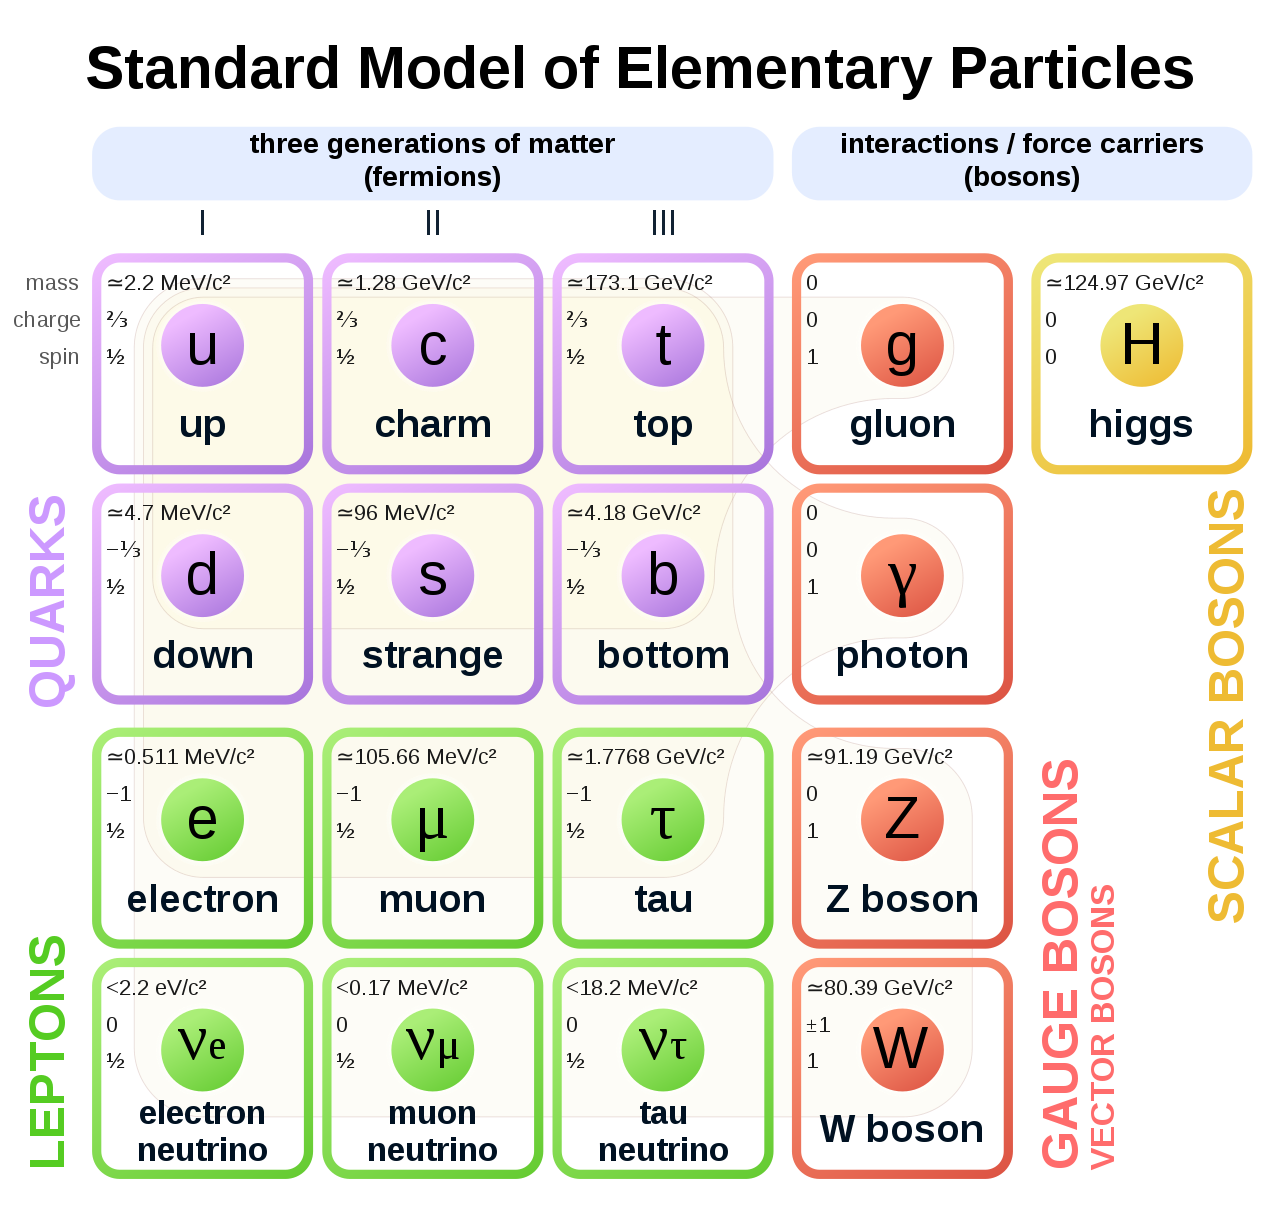
\includegraphics[width=0.5\textwidth]{figures/theory/SM}
\caption{The elementary particles of the standard model.
Figure taken from Ref.~\cite{SMpict}.}
\label{fig:sm_particles}
\end{center}
\end{figure}

%Within the SM, the dynamics of the strong interactions involving quarks and gluons are described by Quantum Chromodynamics (QCD), 

Quarks are fermions with a spin of $1/2$, and carry a fractional electric charge as well as a color charge.
They all have mass and come in six flavors: up, down, strange, charm, top, bottom.
The lightest quarks (u and d) combine and form stable particles, while the heavier quarks can only be produced in energetic environments and decay rapidly.
Gluons are gauge bosons (force carriers) with a spin of $1$, and are what hold quarks together.
The dynamics of the quarks and gluons, collectively referred to as partons are described by the QCD Lagrangian given by \cite{Beringer:1481544}:

\begin{align}
\mathcal{{L}}_{\mathrm{QCD}} = \sum_q \bar{\psi}_{q,a} (i \gamma^\mu \partial_\mu \delta_{ab} - g_s \gamma^\mu t_{ab}^C \mathcal{A}_\mu^C - m_q \delta_{ab}) \psi_{q,b} - \frac{1}{4} F_{\mu\nu}^A F^{A \mu\nu}
\end{align}
where $\psi_{q,a}$ and $\psi_{q,b}$ are quark-field spinors for a quarks with flavor $q$, mass $m_q$, and color $a$ and $b$ respectively, with the values for $a$ and $b$ ranging  from 1 to 3 (for the three colors).
The $\mathcal{A_\mu^C}$ corresponds to the gluon field with $C$ taking values from 1 through 8 (for the 8 types of gluons).
The $t_{ab}^C$ corresponds to the Gell-Mann matrices that are the generators of the SU(3) group, and dictate the rotation of the quarks color in SU(3) space when it interacts with a gluon.
The coupling constant is encoded within $g_s$, which is defined by $g_s \equiv \sqrt{4 \pi \alpha_s}$.
The field tensor $F_{\mu\nu}^A$ can be written in terms of the structure constants of the SU(3) group $f_{ABC}$, and is given by:

\begin{align}
F_{\mu\nu}^A = \partial_\mu \mathcal{A}_\nu^A - \partial_\nu \mathcal{A}_\mu^A - g_s f_{ABC} \mathcal{A}^B \mathcal{A}^C
\end{align}
While many parallels can be drawn between Quantum Electrodynamics (QED, the theory that describes photons and electrons) and QCD, the main difference between the two comes from the gluon-gluon interactions allowed in QCD, making it non-Abelian.
These interactions can be summarized as shown in Figure \ref{fig:qcd_diagrams}.

\begin{figure}[htbp]
\begin{center}
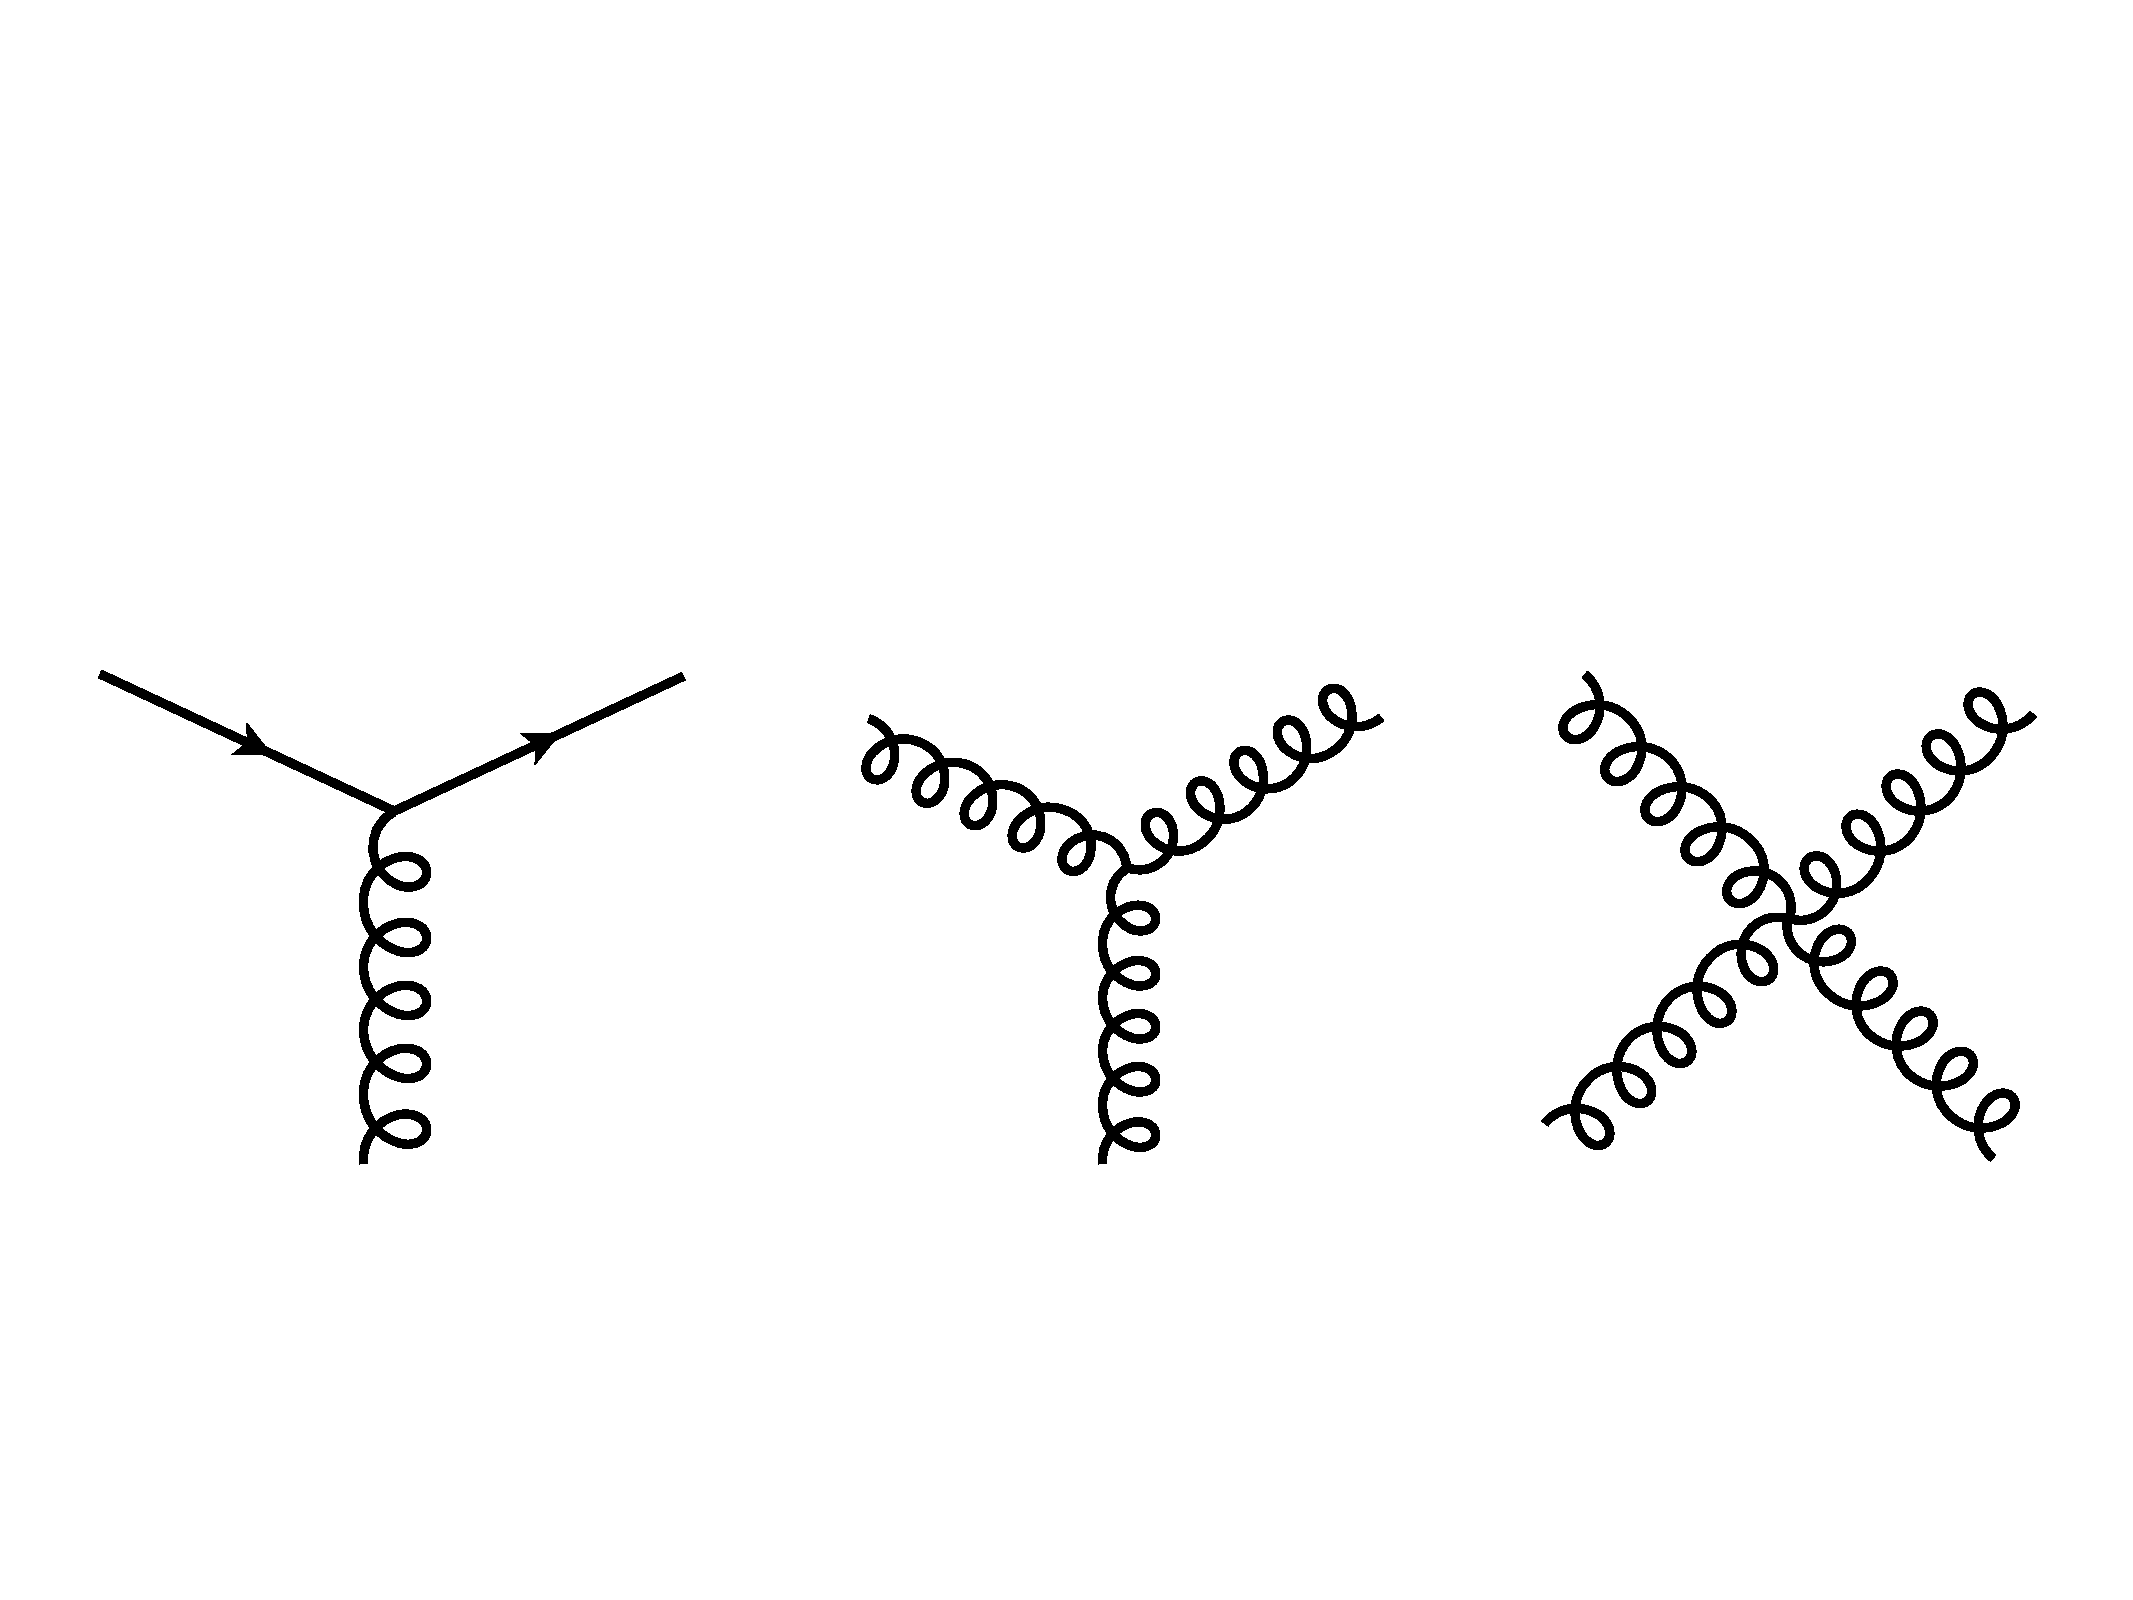
\includegraphics[width=0.8\textwidth]{figures/theory/qcd_diagrams}
\caption{The allowed vertices in QCD.
The vertices involving two or more gluons are unique to QCD and do not have a QED analog.}
\label{fig:qcd_diagrams}
\end{center}
\end{figure}

A core feature of QCD is that the coupling constant \alphas\ has an energy dependence shown in Figure~\ref{fig:running_coupling}.

\begin{figure}[htbp]
\begin{center}
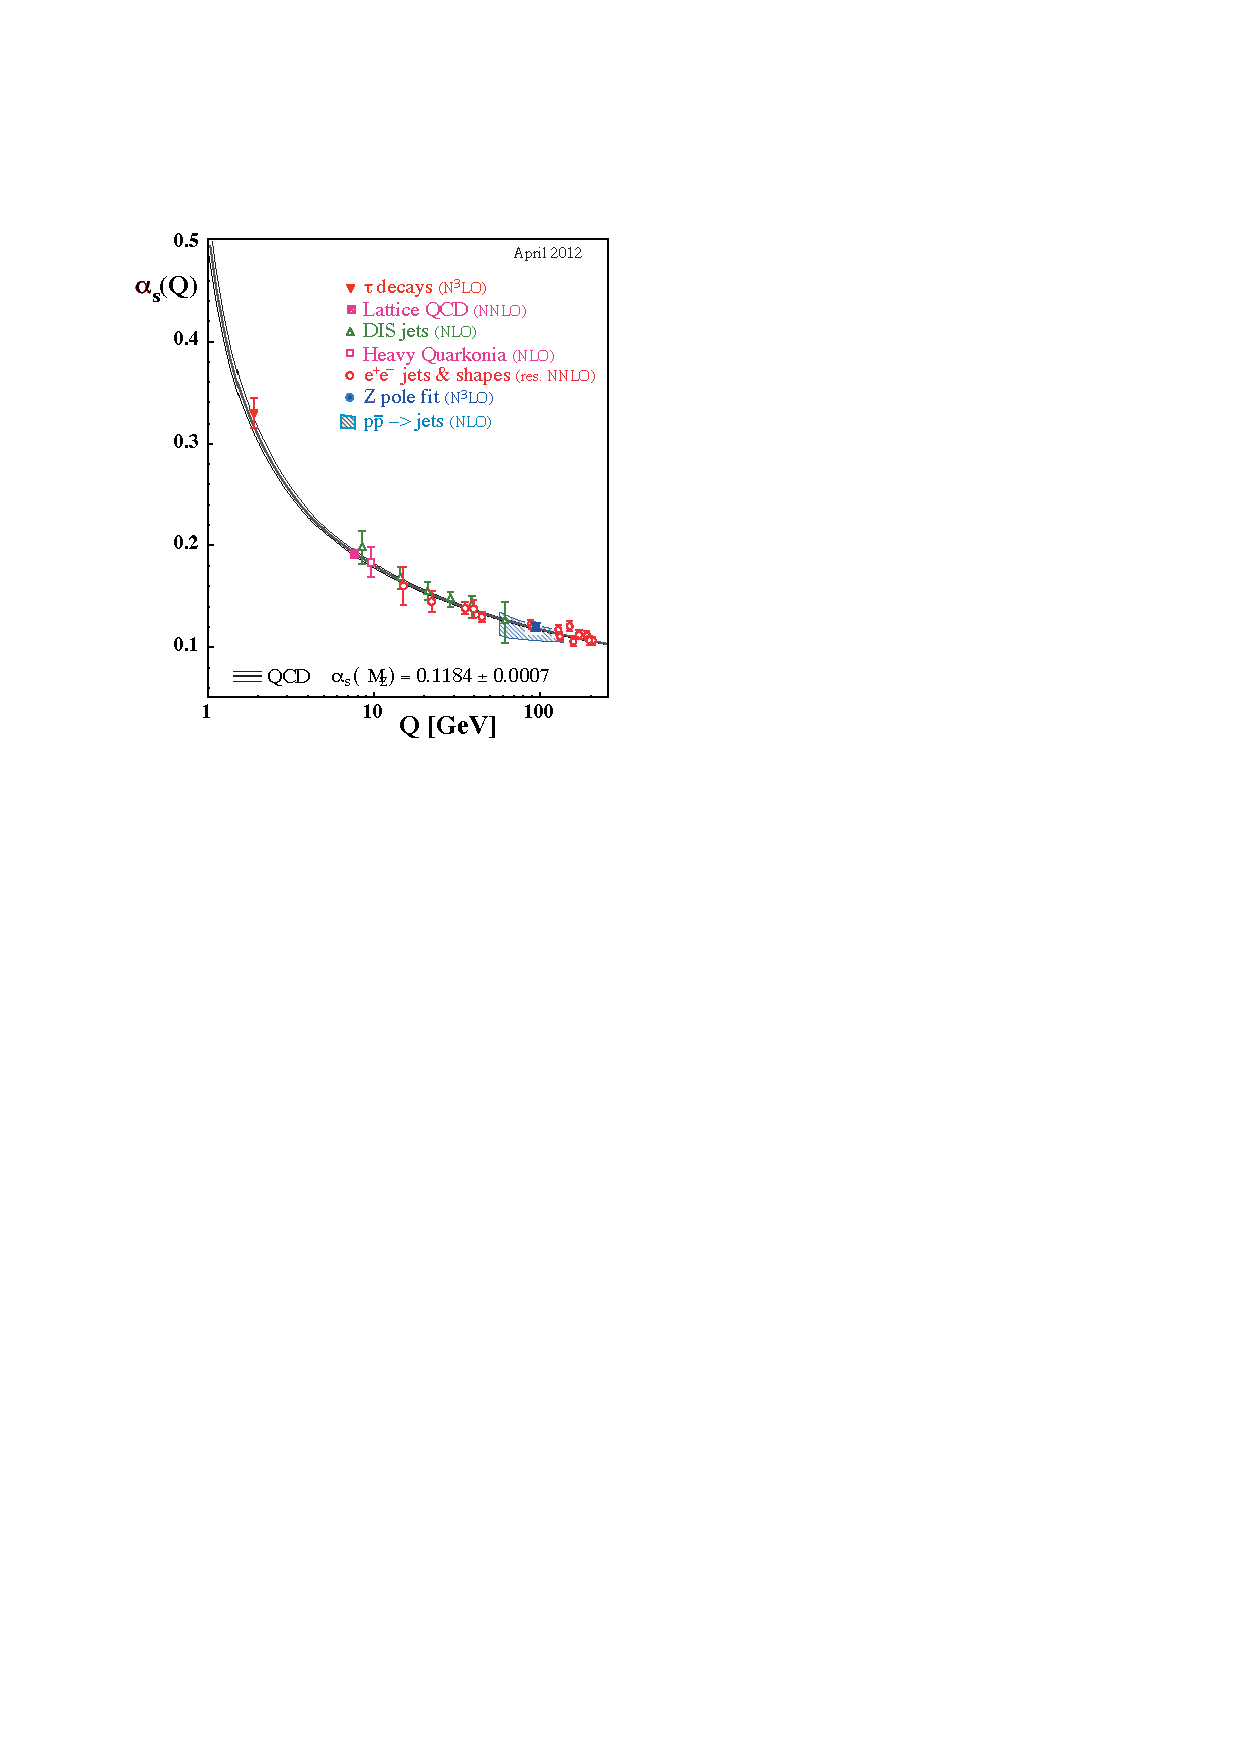
\includegraphics[width=0.5\textwidth]{figures/theory/running_coupling}
\caption{The running coupling constant $\alpha_s$ as a function of the momentum transfer $Q$.
Figure taken from Ref.~\cite{Beringer:1481544}.}
\label{fig:running_coupling}
\end{center}
\end{figure}

This dependence can be expressed in terms of the $\beta$ function as

\begin{align}
Q^2 \frac{\partial \alpha_s (Q^2)}{\partial Q^2} = \beta(\alpha_s (Q^2))
\end{align}
where $Q$ is the momentum transfer in the particle reaction
\footnote{The momentum transfer $Q$ is the amount of momentum transferred in a scattering process.}.
The beta function can be expressed using perturbative QCD (pQCD) as:

\begin{align}
\beta( \alpha_s ) = - (b_0 \alpha_s^2 + b_1 \alpha_s^3 + b_2 \alpha_s^4...)
\end{align}
where the coefficients $b_i$ depend on the number of colors and flavors.
This running coupling constant is small and asymptotically tends to zero at large energy scales (or at small distances) and is large at small energy scales (large distances).
This running coupling phenomenon leads to two key behaviors: asymptotic freedom and color confinement.


\subparagraph{Asymptotic Freedom: }
At high energy scales (small distances), the QCD coupling constant $\alpha_s$ is small and tends to zero, implying a free particle behavior of quarks and gluons\cite{PhysRevLett.30.1343, PhysRevD.8.3633}.
This has been observed by a variety of deep inelastic scattering (DIS) experiments \cite{Deur:2014vea, Kim:1998kia, Altarelli:1996nm, RevModPhys.63.597, Kataev:2001kk, Alekhin:2012ig, Alekhin:2013nua, Blumlein:2006be, Aaron:2007xx, Chekanov:2007pa, Chekanov:2008af, Abramowicz:2010cka, Abramowicz:2010ke, Aaron:2009vs}.
These scattering experiments shown in Figure~\ref{fig:dis_schematic}, probe the interior of a nucleon using highly energetic leptons like electrons. The electron scatters off of the target proton, producing a lepton and a hadron shower. Bu 
First done by MIT-SLAC \cite{PhysRevLett.23.930, PhysRevLett.23.935}, these DIS experiments showed the weak $Q^2$ dependence on the inelastic scattering cross-sections, as well as Bjorken scaling \cite{PhysRev.179.1547}, where the proton structure functions are independent of the momentum transfer.
These experiments revealed the point-like constituents of the proton and paved the road to an asymptotically free theory.

\begin{figure}[htbp]
\begin{center}
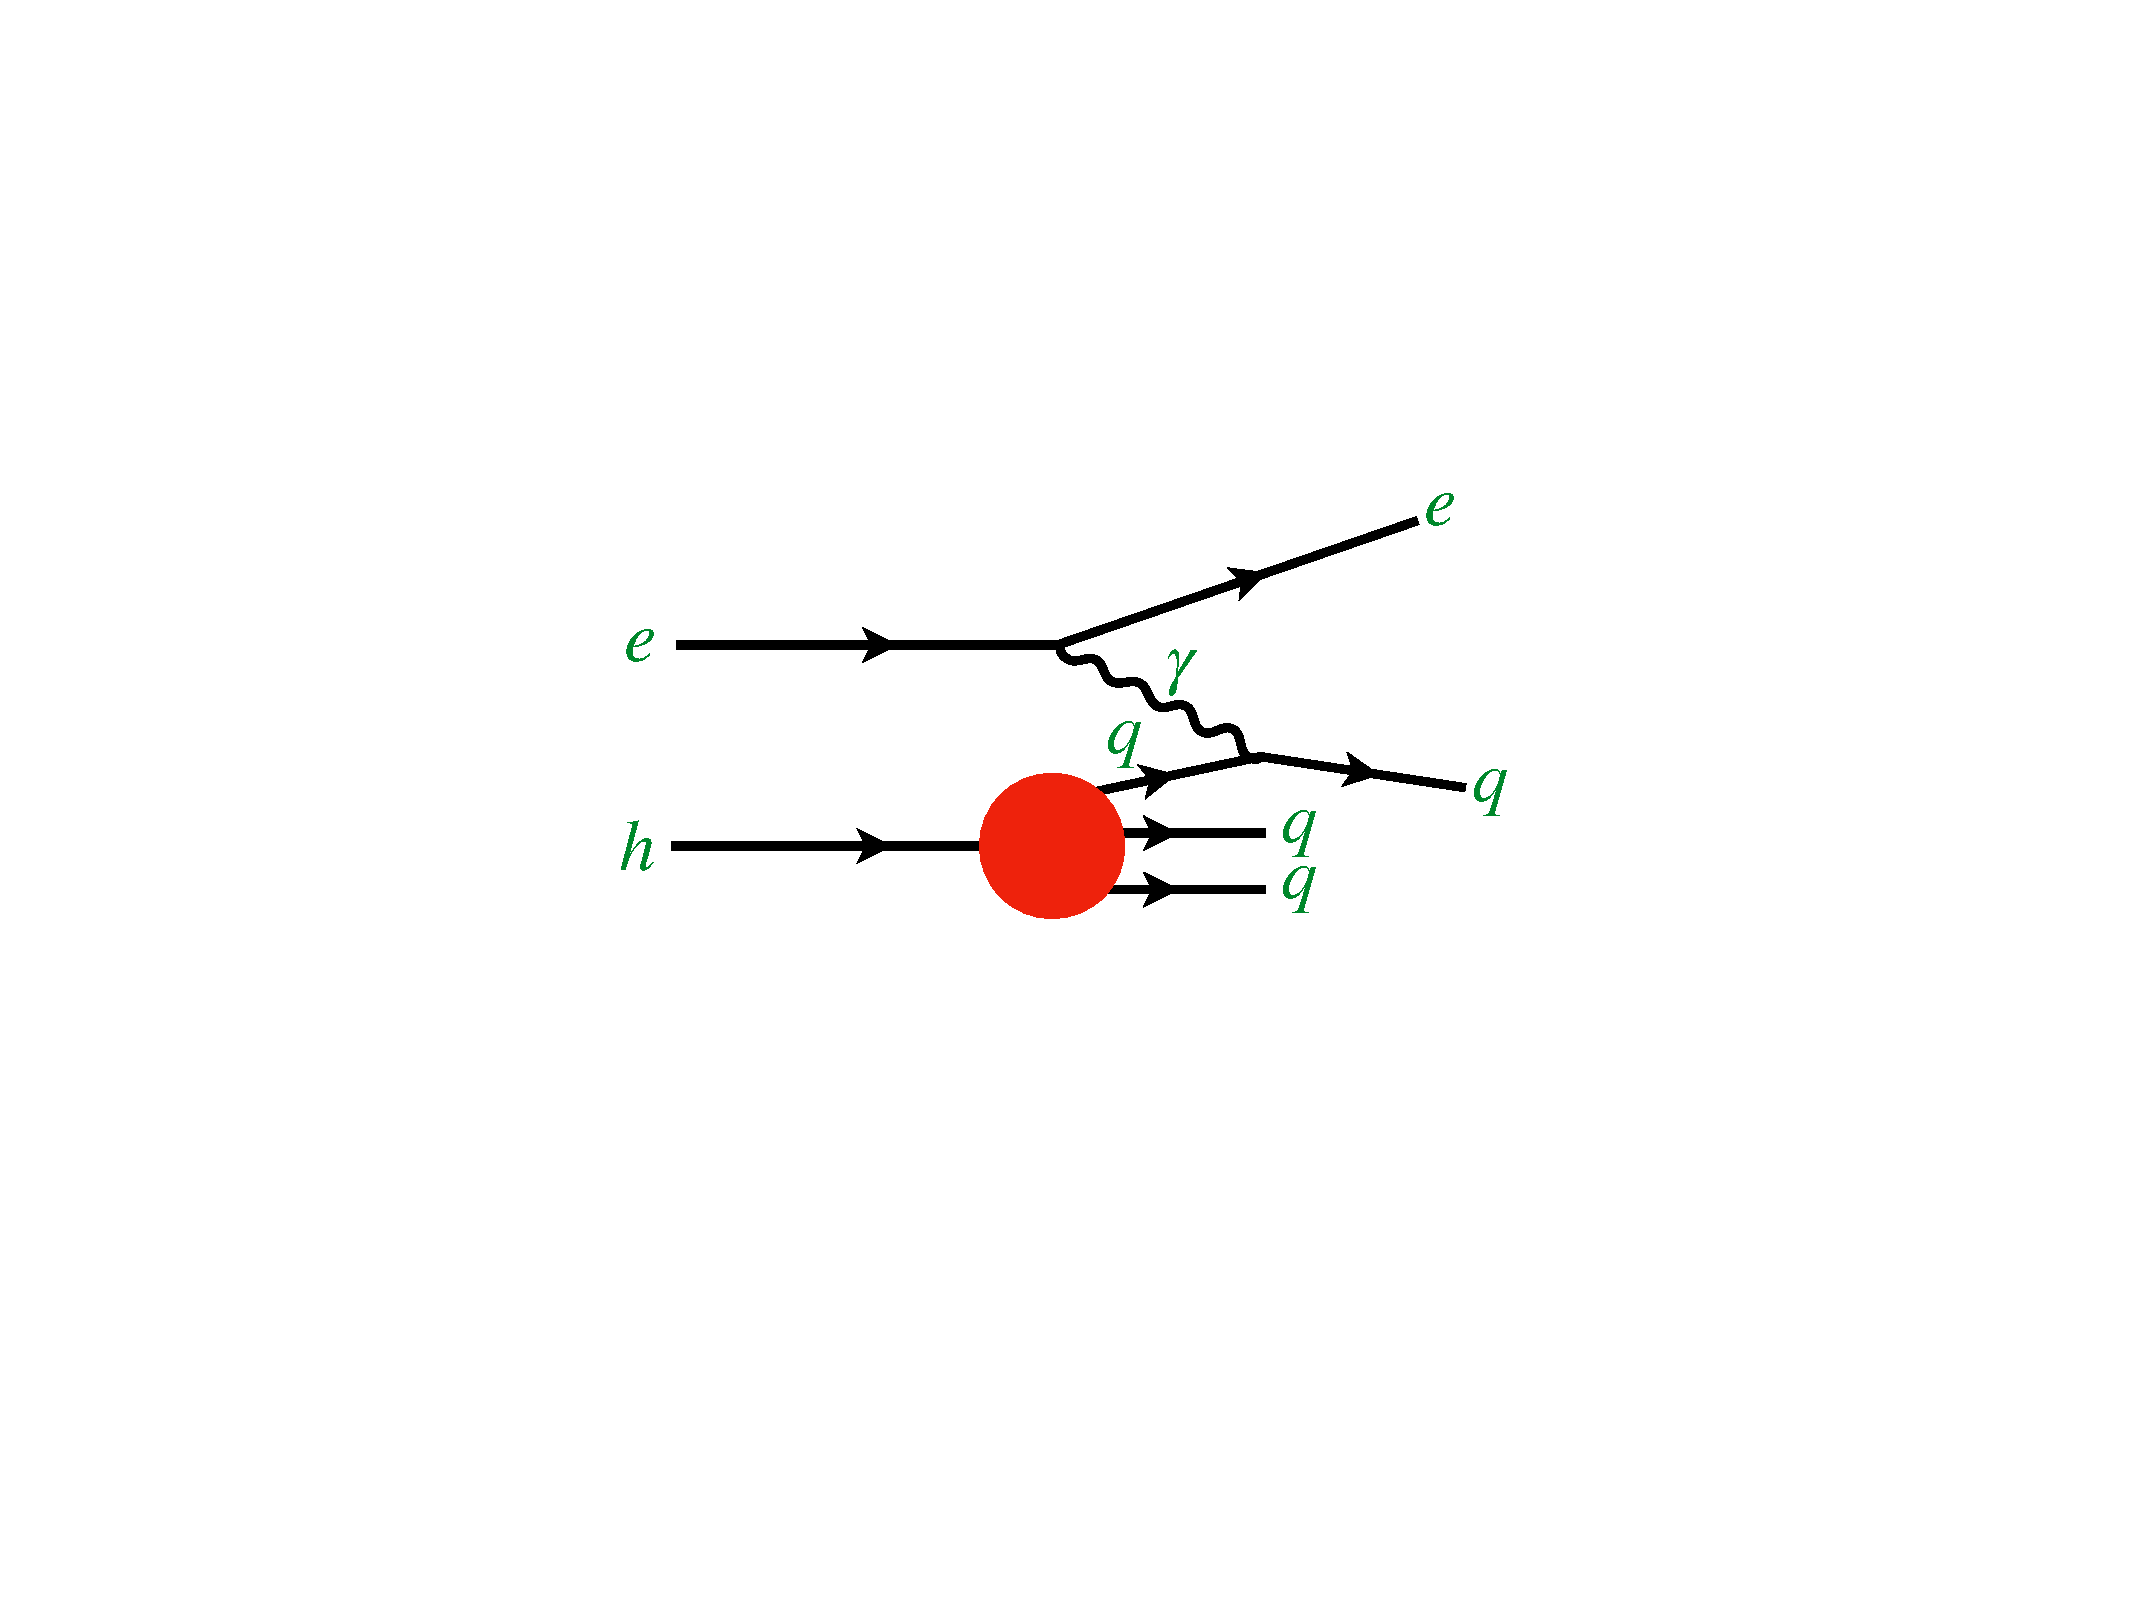
\includegraphics[width=0.35\textwidth]{figures/theory/DIS}
\caption{Schematic of the deep inelastic scattering experiment.}
\label{fig:dis_schematic}
\end{center}
\end{figure}


\subparagraph{Color Confinement}
The opposite end of the running coupling constant phenomenon is color confinement.
Proved to be a consequence of asymptotic freedom in Ref~\cite{Nishijima1996}, this property of QCD described in Ref.~\cite{PhysRevD.10.2445} forbids the direct observation of free quarks and gluons, allowing only for composite particles that are color singlets.
While have been numerous efforts to understand the source of this phenomenon like in Refs.~\cite{BUCHMULLER1982479, KOGUT1976199, PhysRevD.31.2910, PhysRevD.57.2603, PhysRevD.62.114503, RevModPhys.55.775, PhysRevLett.90.102001}, these are based on numerical calculations.
An analytic proof of color confinement still escapes description and in fact, is one of the Millennium Problems \cite{MillenniumProb}.


%\subsection{Parton Distribution Functions}
%Deep ineslatic scattering experiments showed the internal point-like structure of a proton that can be described in terms of probability density functions called parton distribution functions.
%These are written in terms of the longitudinal momentum fraction carried by a constitutent proton, $x$, given as:
%
%\begin{align}
%x = \frac{Q^2}{2 P \dot q} = \frac{Q^2}{2 M \nu}
%\end{align}
%where $\nu$ is the energy of the photon shown in Figure~\ref{fig:dis_schematic}. This can be determined by 




%An analytic proof of the origin of color confinement is described in Ref.\cite{Gao:2018xsg}.
%==========================================================
%
%%QCD allows for predicting a variety of observables in particle reactions involving quarks and gluons in terms of the coupling constant $\alpha_s$.
%QCD amplitudes can be calculated by using the matrix elements for the basic diagrams shown in Figure~\ref{fig:qcd_diagrams} along with the quark and gluon propagators.Perturbative calculations done with the assumption that the coupling constant \alphas $ < 1 $ allow for 
%Another major feature 
% quark and gluon propagators along with teh corre
%
%
%

%The classical QCD Lagrangian is given by \cite{Chyla:2004zz}
%
%\begin{align}
%\mathcal{{L}}_{\mathrm{QCD}} = \sum_q \bar{\psi}_{q,a} (i \gamma^\mu \partial_\mu \delta_{ab} - g_s \gamma^\mu t_{ab}^C \mathcal{A}_\mu^C - m_q \delta_{ab}) \psi_{q,b} - \frac{1}{4} F_{\mu\nu}^A F^{A \mu\nu}
%\end{align}
%
%%\begin{align}
%%\mathcal{{L}}_{\mathrm{QCD}} &= \mathcal{L}_g + \mathcal{L}_q \\
%%&=  -\frac{1}{4} F_{\mu\nu} F^{\mu\nu} + \bar{\Psi}(i  \slashed{\partial} - m_q) \Psi + g \bar{\Psi} \gamma_\mu T \Psi A^\mu
%%\end{align}
%
%\begin{align}
%\mathcal{{L}}_{\mathrm{QCD}} =  -\frac{1}{4} F_{\mu\nu} F^{\mu\nu} + \bar{\Psi}(i  \slashed{\partial} - m_q) \Psi + g \bar{\Psi} \gamma_\mu T \Psi A^\mu
%\end{align}
%
%\begin{align}
%F^{\mu\nu}_a (x) \equiv \frac{\partial A_a^\nu (x)}{\partial x_\mu} - \frac{\partial A_a^\mu (x)}{\partial x_\nu}
%\end{align}
%
%%This Lagrangian is can be thought of as the sum of the quark and gluon terms $\mathcal{L}_g$ and $\mathcal{L}_q$, where
%%\begin{align}
%%\mathcal{L}_g &= - \frac{1}{4}\frac{1}{4} F_{\mu\nu} F^{\mu\nu} 
%%\end{align}
%
%
%where $Q$ is the momentum transfer in the particle reaction.This running coupling constant is small and asymptotically tends to zero at large energy scales (or at small distances) and is large at small energy scales (large distances).This can be seen in Figure \ref{fig:running_coupling}, which shows the $\alpha_s$ dependence on $Q$.This running coupling leads to two key behaviors discussed below.
%
%
%
%

\section{Quark-Gluon Plasma in Heavy Ion Collisions}
\label{sec:qgp_hi}
% !TEX root = thesis-ex.tex

The quark-gluon plasma is a state of matter that is comprised of free partons and is formed in extreme conditions of temperature and pressure \cite{SHURYAK198071}.
First discovered in heavy ion collisions at the Relativistic Heavy Ion Collider (RHIC) \cite{ARSENE20051, Adcox:2004mh, ADAMS2005102, Back:2004je}, its study is motivated by the fact that is the only way to access the dynamics of partons that are otherwise confined within hadrons.


A schematic of a heavy ion collision is shown in Figure~\ref{fig:qgp_form}.
The colliding nuclei have a relativistic $\gamma$ factor of approximately 3000 and form discs.
As they collide, color fields from the partons within the colliding nuclei interact and fill the space between them.
The energy density in the collision depends on the number of colliding nucleons and the collision energy, and can range from 1 GeV/fm$^3$ for $\sqrtsnn = 7.7$ GeV at the lower limit of RHIC energies \cite{PhysRevC.93.024901} to 15 GeV/fm$^3$ for $\sqrtsnn = 5.02$ TeV at the Large Hadron Collider (LHC) \cite{PhysRevC.94.034903, PhysRevLett.109.152303, Jiang:2018wzu}.
This is well above the $0.2 - 1 \rm{GeV}/\rm{fm}^3$ energy density range required to form the QGP \cite{Karsch2002, PhysRevD.90.094503}.
After the collision the QGP cools and expands and the energy density between the receding nuclei starts to decrease.
At a certain critical temperature about 1-10 fm/c after the collision, the energy density decreases to lower than what is within a hadron, and the plasma forms a hadron gas \cite{doi:10.1146/annurev.nucl.46.1.71}.
This process, referred to as a chemical freeze-out, occurs at about 160 MeV \cite{Fodor_2004, ADAMS2005102, PhysRevC.93.024917, Borsanyi:2010bp}.
The hadrons within the gas have energies below the threshold for inelastic particle production but briefly scatter off of each other resulting in modifications to their momentum spectra.
This continues till the medium cools further and reaches what is called a thermal freeze-out at 100--150 MeV, at which point the hadrons fly freely towards the detector \cite{PhysRevC.69.024904, PhysRevC.72.014908, PhysRevC.75.024910, PhysRevC.88.044910}.

\begin{figure}[htbp]
\begin{center}
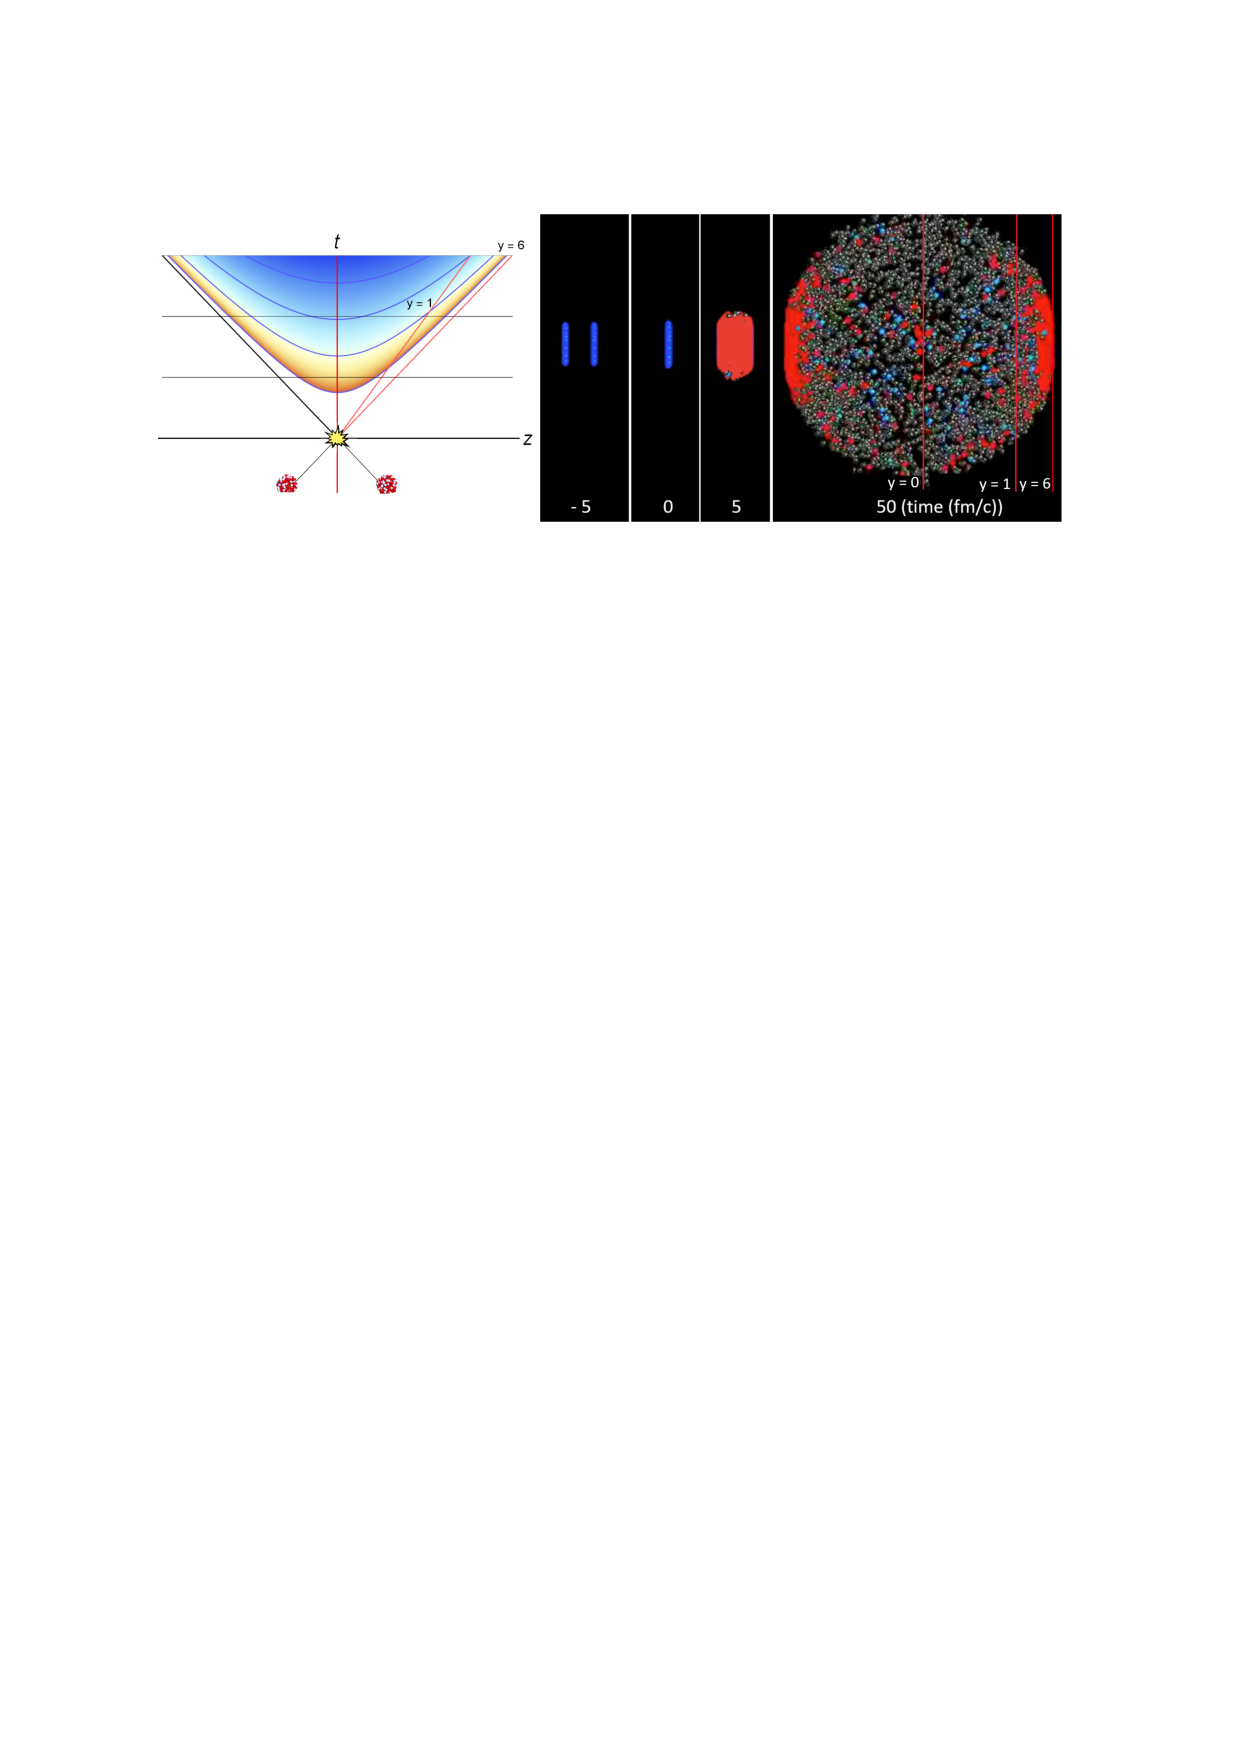
\includegraphics[width=0.85\textwidth]{figures/theory/qgp_formation}
\caption{(left) Space-time diagram for a heavy ion collision.
The color is indicative of the temperature of the QGP formed.
(right) Snapshots of a heavy ion collision at $\sqrtsnn = 2.76$ TeV at different times.
The Lorentz contracted nuclei are in blue while the QGP is in red.
Figure from Ref.~\cite{Busza:2018rrf}.}
\label{fig:qgp_form}
\end{center}
\end{figure}

It is important to note that the impact parameter of the colliding nuclei plays a significant role in the dynamics of the QGP that is formed.
This can be seen in Figure~\ref{fig:collision_centrality}, where the shape and size of the QGP produced for head-on (``central'') collisions is different from that in more glancing (``peripheral'') collisions.

The QGP was initially thought to be a weakly coupled parton gas because of asymptotic freedom from QCD.
The highly energetic collisions such as those at the LHC would imply weak interactions between the partons that make up the plasma \cite{PhysRevLett.34.1353, heinz2013collective, 10.1007/978-1-4020-2705-5_14}.
This would result in rare scatterings between the constituents of the hadron gas formed in such a collision, washing out any spatial anisotropies from the ``'lumpy''-ness of the colliding nuclei.
A strong coupling within the QGP however, would result in the pressure gradients in the medium and spatial anisotropies would be transformed to momentum anisotropies in the particles produced as shown in Figure~\ref{fig:overlap} \cite{Busza:2018rrf}.
In this picture, the non-uniform structure of the colliding nuclei would cause a momentum anisotropy \cite{Ster:1999ib} that would be further enhanced when looking at collisions that are less central and do not have perfect overlap between the colliding nuclei \cite{Poskanzer:1999ea, Pinkenburg:1999ya}.
These observations were seen in azimuthal correlation measurements implying that the medium is indeed strongly coupled \cite{Aaboud:2018ves, PhysRevLett.91.182301, Sirunyan:2017fts, PhysRevLett.116.132302}.

\begin{figure}
\centering
\begin{minipage}[b]{0.45\textwidth}
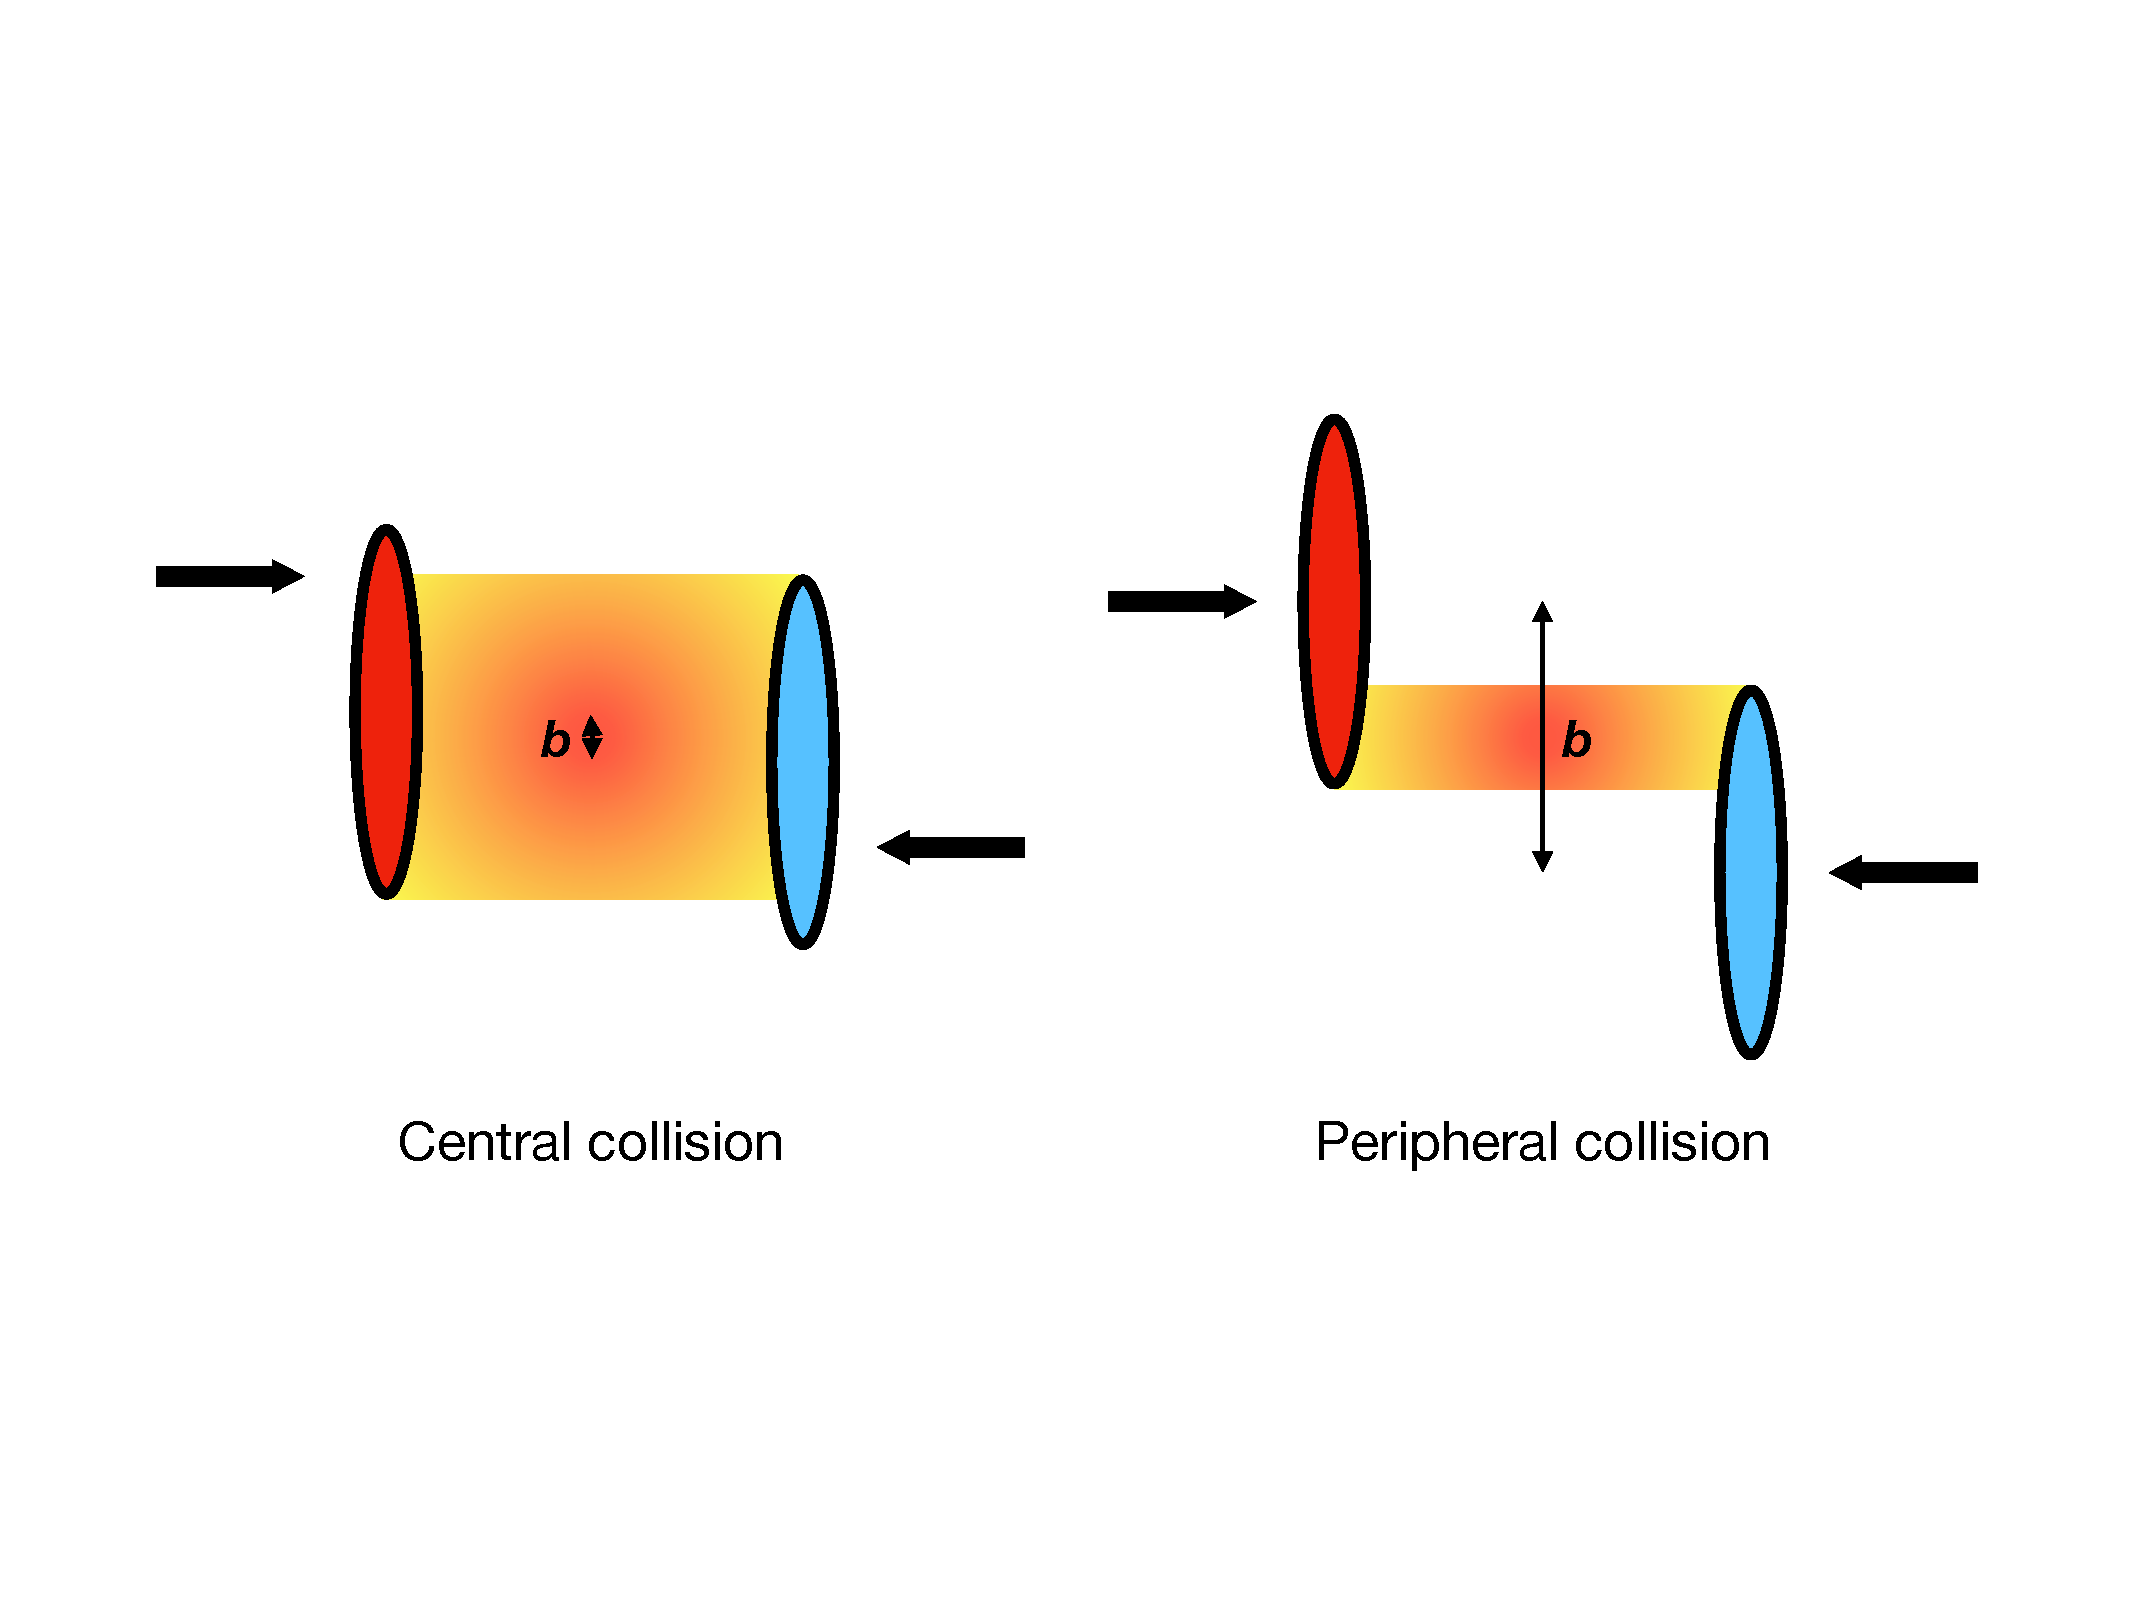
\includegraphics[width=1.\textwidth]{figures/theory/collision_centrality}
\caption{A schematic of central (left) and peripheral (right) heavy ion collisions.
The impact parameter is given by $b$.}
\label{fig:collision_centrality}
  \end{minipage}
 \qquad 
  \begin{minipage}[b]{0.45\textwidth}
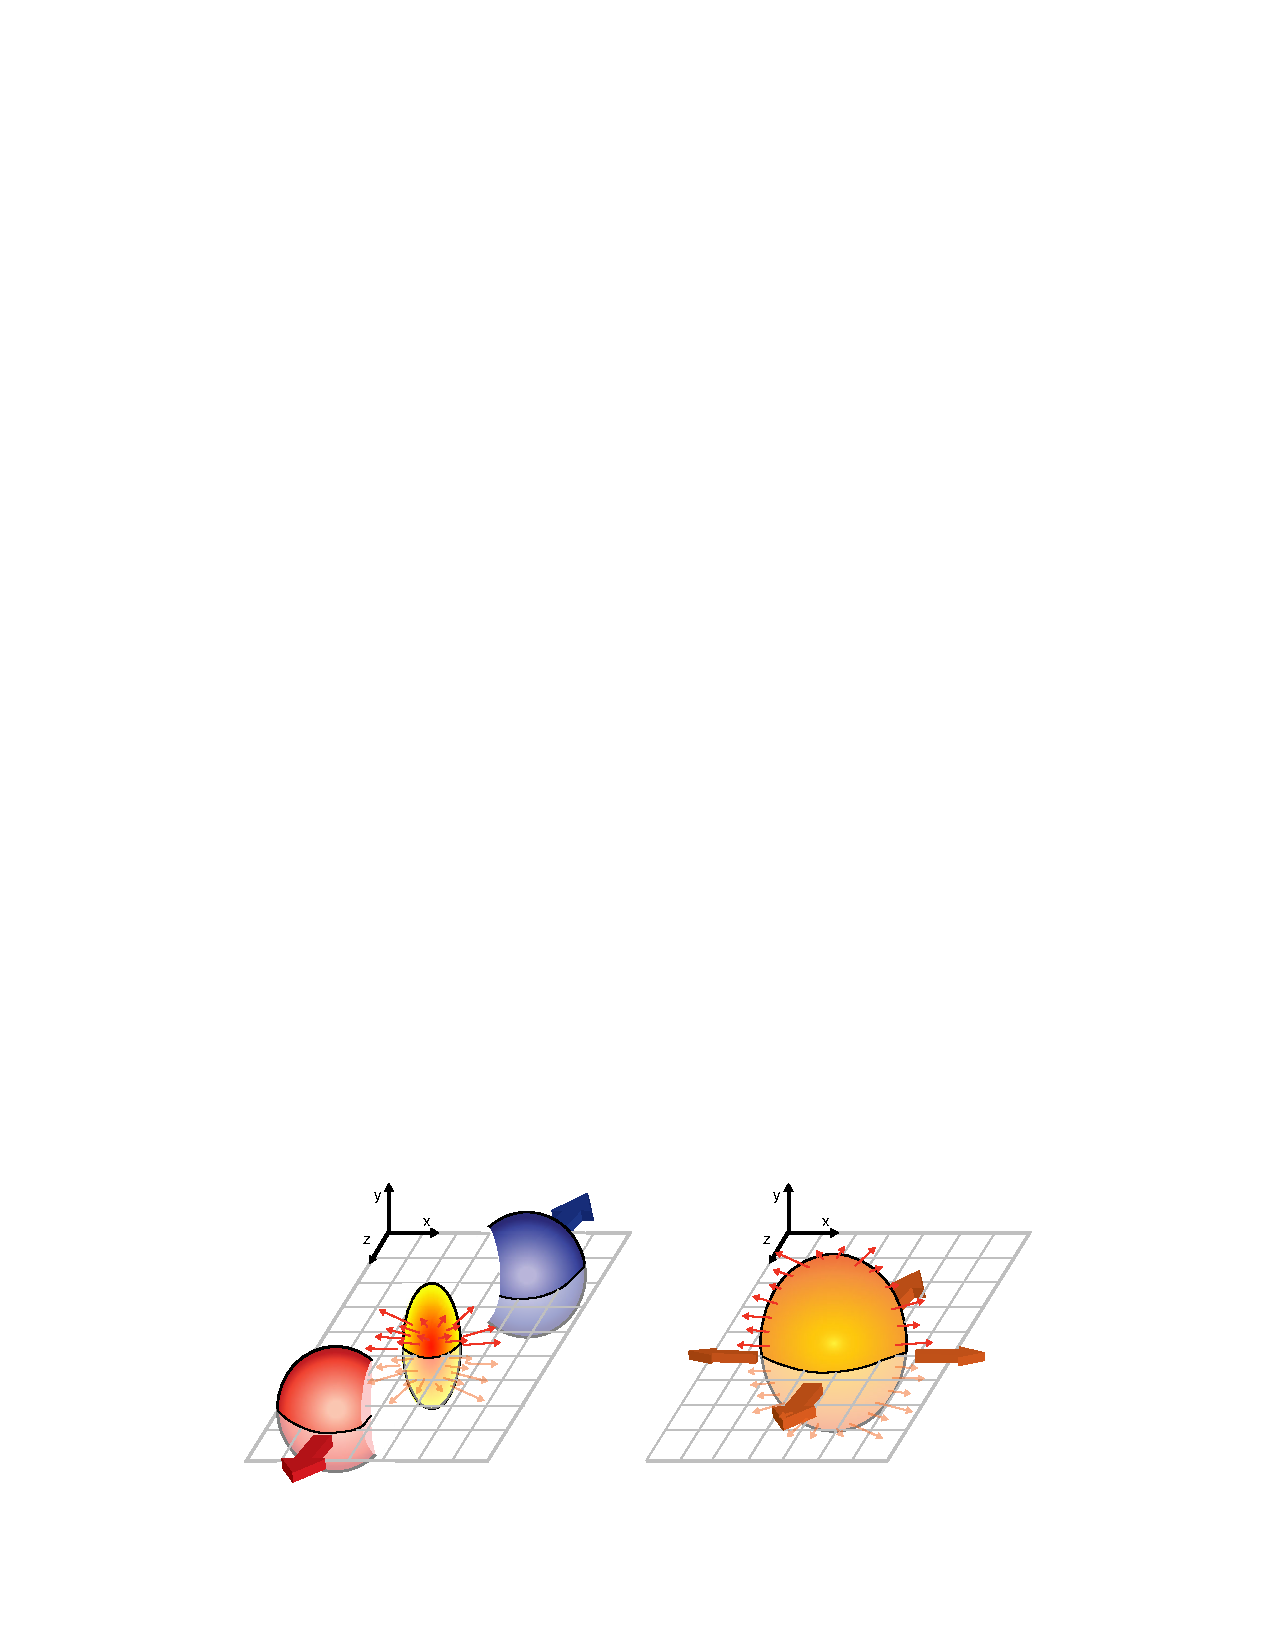
\includegraphics[width=1.\textwidth]{figures/theory/overlap}
\caption{A schematic of the initial overlap region (left) and final spatial anisotropy generated (right).
Figure from Ref.~\cite{RevModPhys.90.025005}.}
\label{fig:overlap}
\end{minipage}
\end{figure}


Properties of the QGP have been successfully described by relativistic hydrodynamic models. 
In fact, such models describing photon emission have been used to explain the data measured at both RHIC \cite{PhysRevLett.104.132301} and LHC \cite{2016235} energies and have suggested that the initial temperature of the QGP is 300--600 MeV \cite{PhysRevC.81.034911}.
The hydrodynamic nature of the QGP can be further quantified by studying the azimuthal angular distribution of particles produced in a heavy ion collision \cite{Poskanzer:1998yz, Teaney:2001av, HIRANO2006299}.
These distributions can be expanded in a Fourier series as: 

\begin{align}
\frac{d\bar{N}}{d\phi} = \frac{N}{2\pi} \left( 1 + 2 \sum_{n=1}^{\infty} v_{n} \cos(n(\phi-\Psi_n)) \right).
\end{align}
where  $N$ is the particle yield, $\phi$ is the azimuthal angle in the transverse plane and $\Psi_n$ is the orientation of the $n^{\mathrm{th}}$ order symmetry plane and is called the reaction plane.
The reaction plane, along with the participant plane, are shown in Figure~\ref{fig:reaction_plane}.
The coefficient $v_n = \langle \cos[n(\phi_i - \Psi_n)] \rangle$ is the magnitude of the $n^{\rm{th}}$ order azimuthal anisotropy, and is referred to as the flow harmonic.
The first harmonic $v_1$ is called directed flow because it indicates a particular direction, while the second harmonic $v_2$ is called elliptic flow since the azimuthal distribution in polar coordinates for $v_2 \neq 0$ is an ellipse.
These are shown in Figure~\ref{fig:flow_v1_v2}.
The azimuthal correlations that are a result of flow can be described by relativistic hydrodynamics.
A comparison of anisotropies measured in terms of $v_n$ in Ref.~\cite{ALICE:2011ab} and a hydrodynamic model described in Ref.~\cite{Niemi:2015qia} is shown in Figure~\ref{fig:flow_coeff}.


\begin{figure}
\begin{center}
  \begin{minipage}[b]{0.45\textwidth}
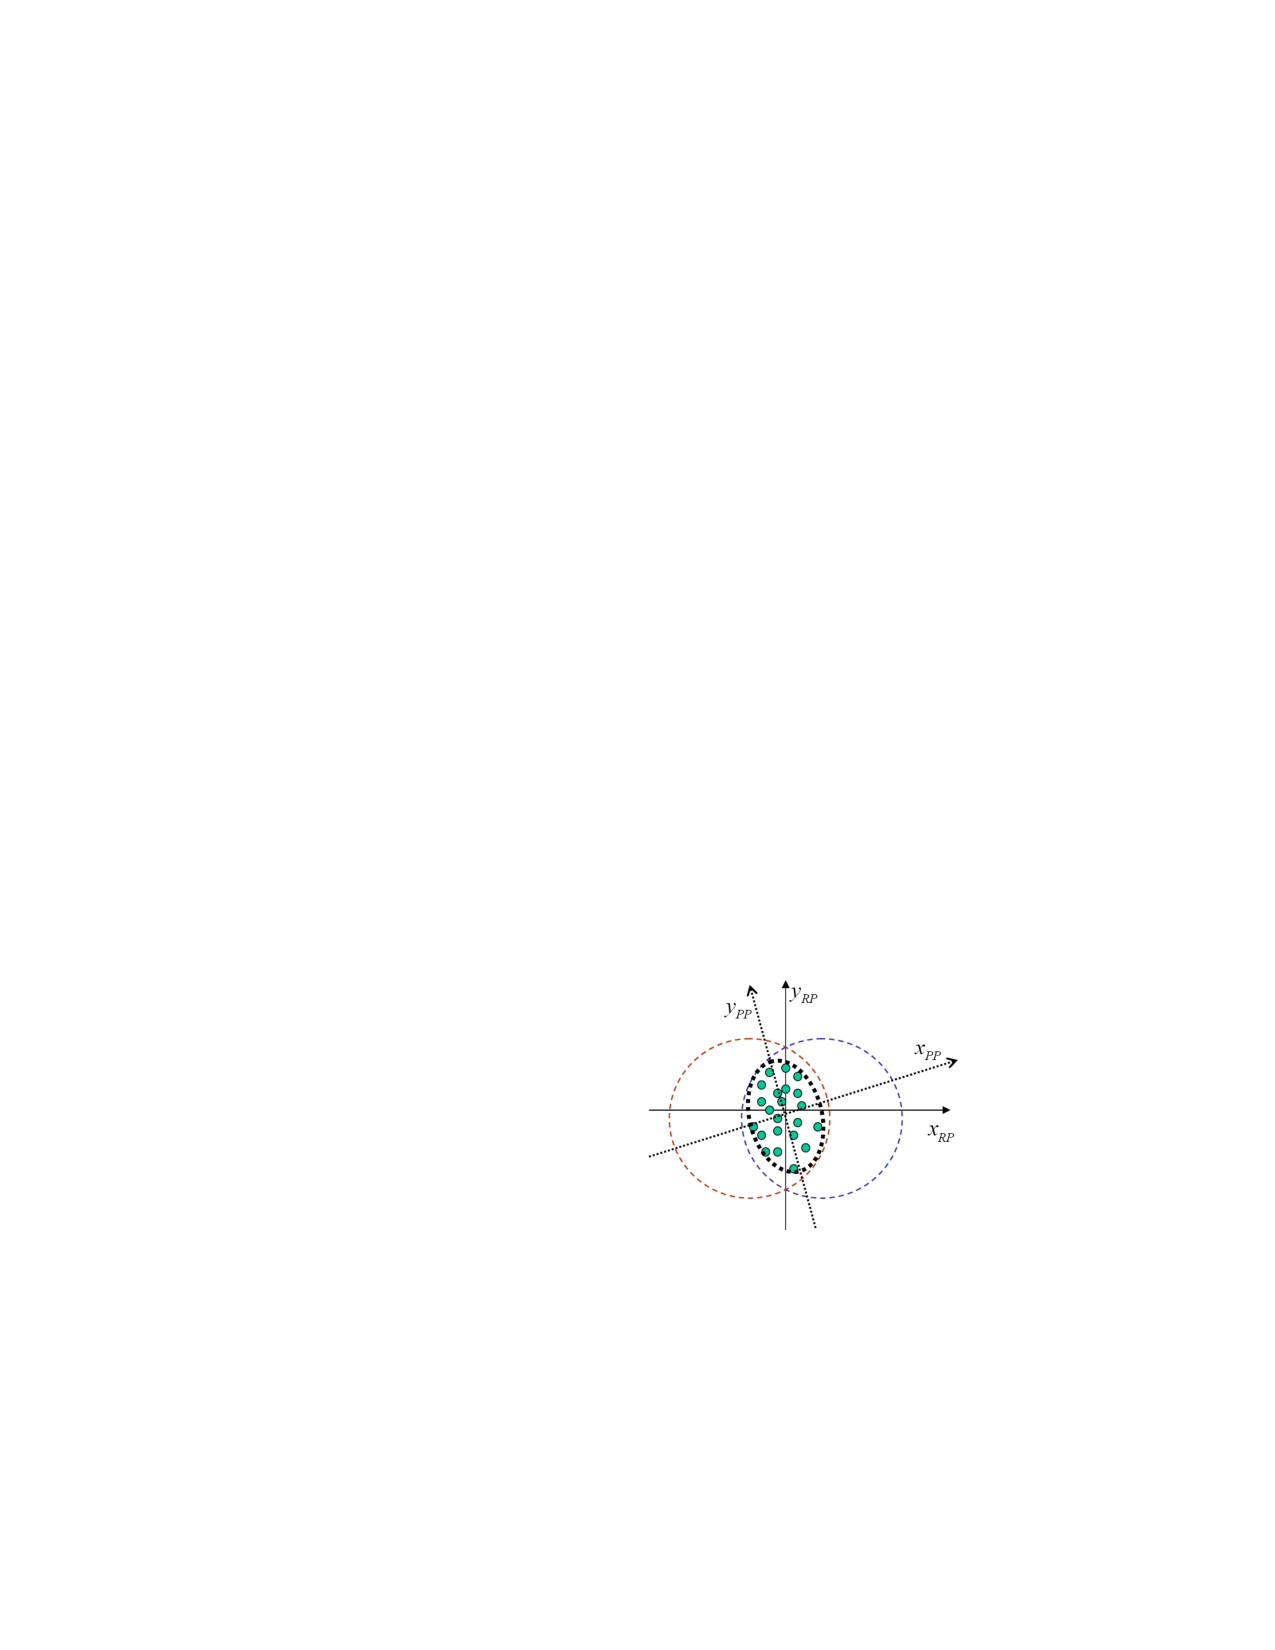
\includegraphics[width=\textwidth]{figures/theory/reaction_plane}
\caption{Definitions of the Reaction and Participant Plan coordinate systems.
Figure from Ref.~\cite{Voloshin:2008dg}.}
\label{fig:reaction_plane}
  \end{minipage}
 \qquad
 \begin{minipage}[b]{0.45\textwidth}
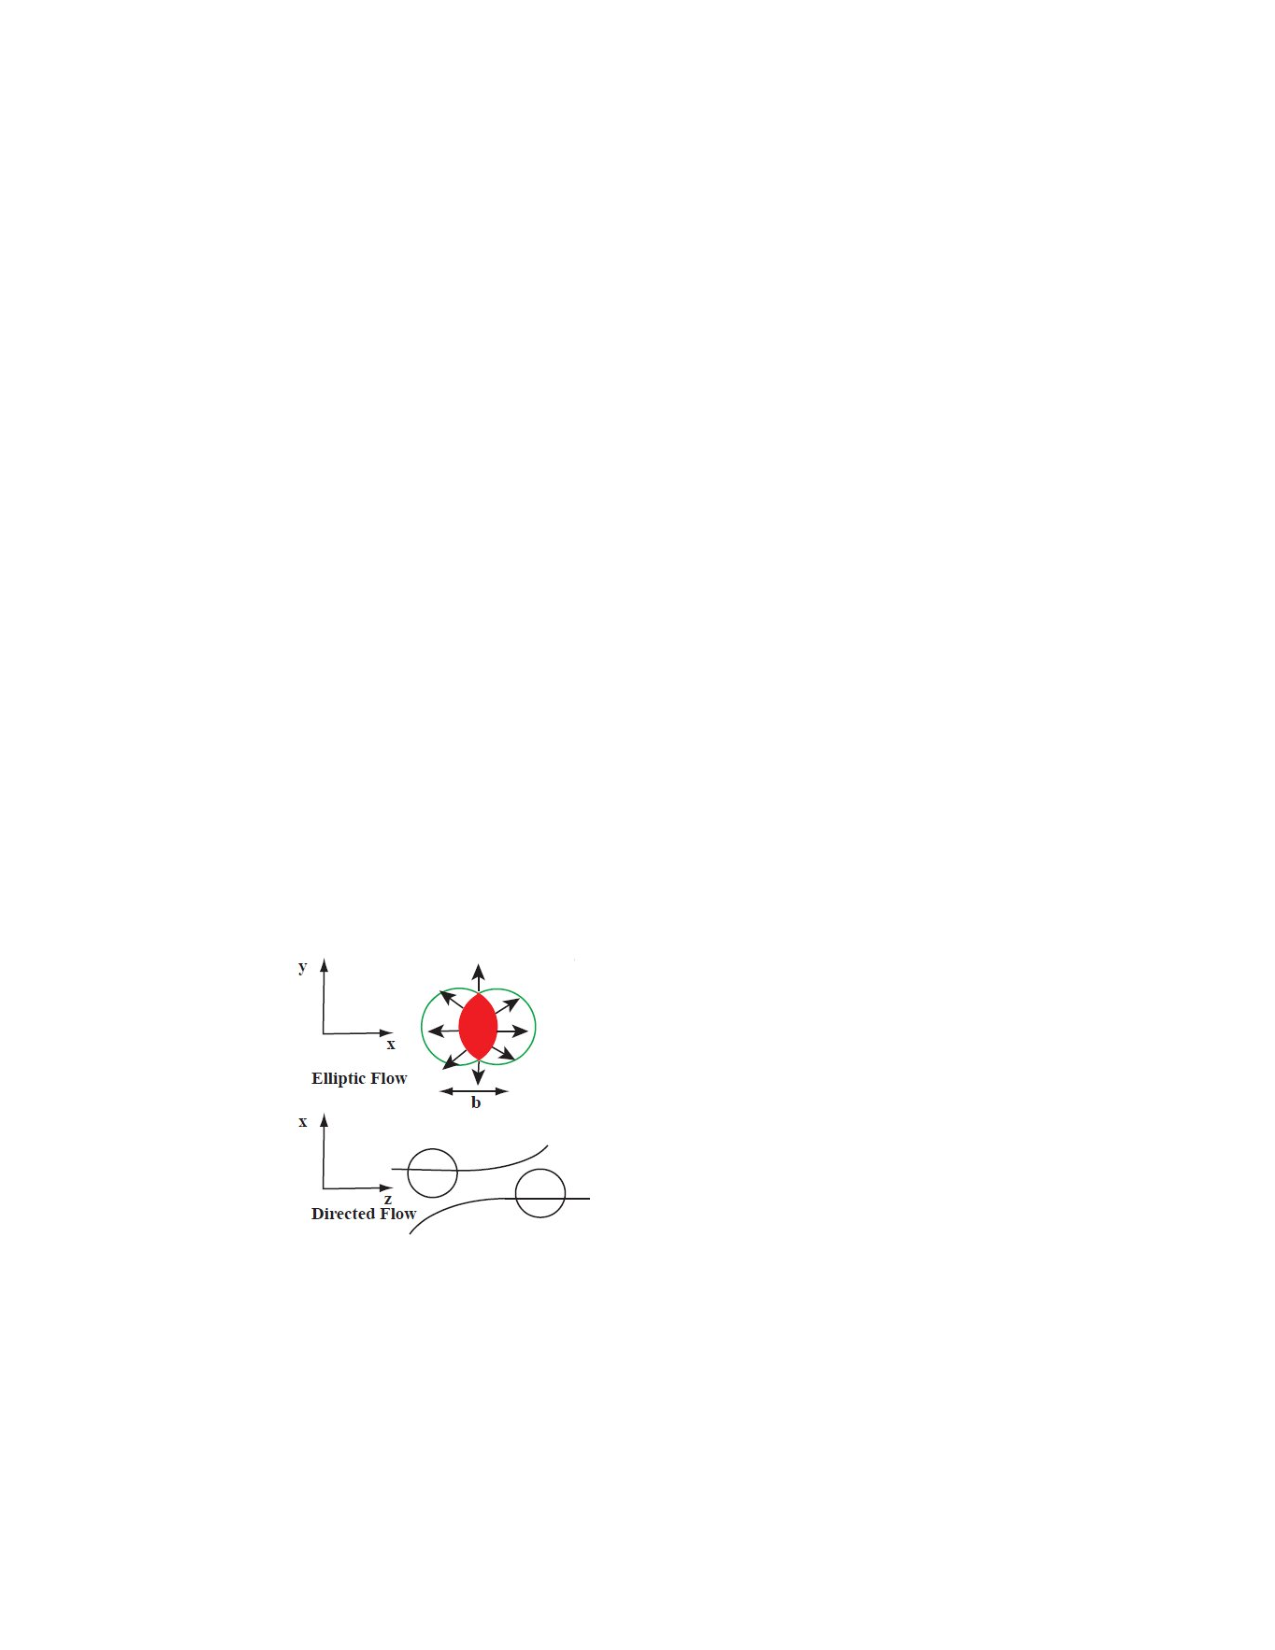
\includegraphics[width=\textwidth]{figures/theory/flow_v1_v2}
\caption{Schematics of elliptic and directed flow.
Figure from Ref.~\cite{Voloshin:2008dg}.}
\label{fig:flow_v1_v2}
  \end{minipage}
  \end{center}
\end{figure}

\begin{figure}[htbp]
\begin{center}
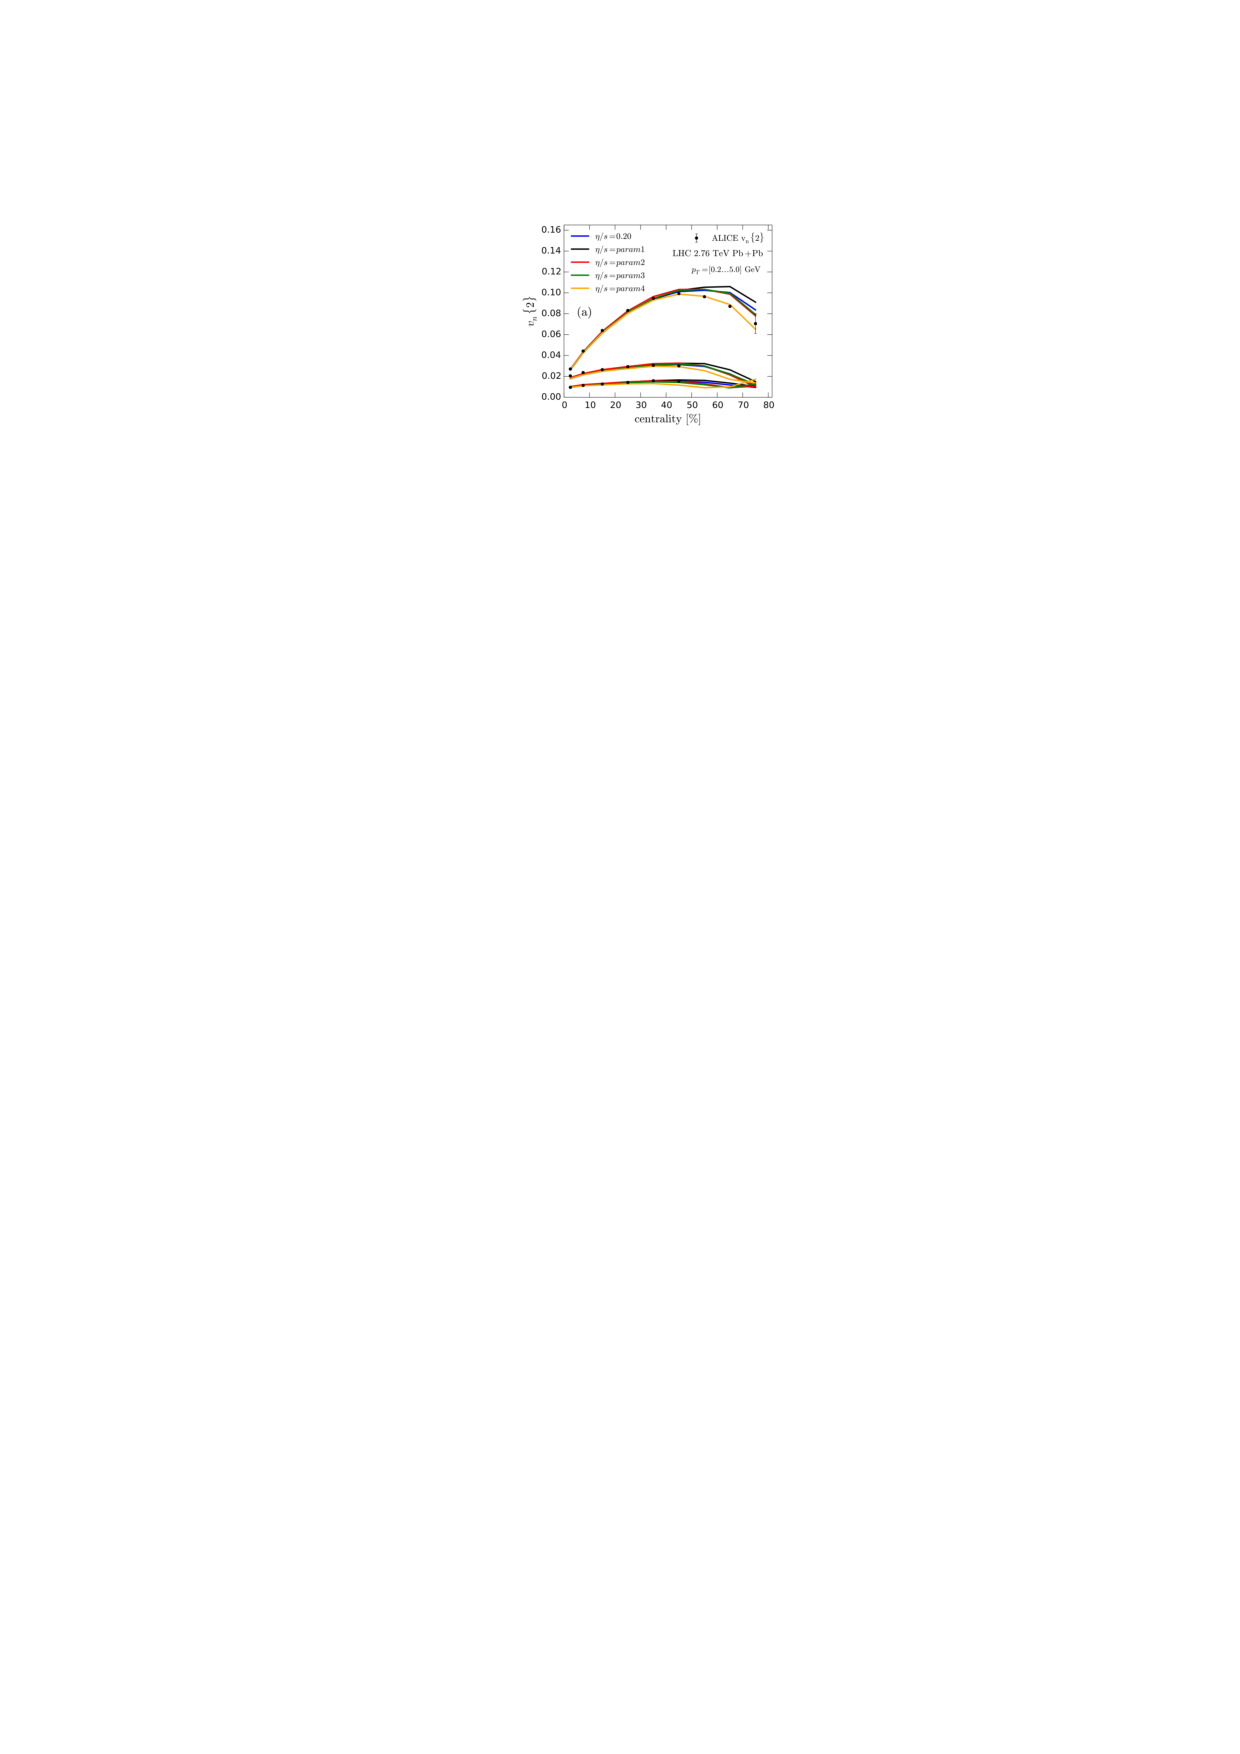
\includegraphics[width=0.45\textwidth]{figures/theory/flow_coefficients}
\caption{Comparison of a hydrodynamic model from Ref.~\cite{Niemi:2015qia} to anisotropy measurements by ALICE \cite{ALICE:2011ab} for different parameterizations of $\eta / s $ and for different $v_n$, {\it{n}} = 2, 3, 4 from top to bottom, as a function of collision centrality.
Figure from Ref.~\cite{Busza:2018rrf}.}
\label{fig:flow_coeff}
\end{center}
\end{figure}

The measured anisotropies can be used to constrain the specific viscosity given by the ratio of viscosity to entropy density, $\eta / s$, and have shown that the QGP is a near perfect liquid with an $\eta / s$ of near the theoretical minimum of $1/4\pi$ \cite{ARSENE20051, GYULASSY200530}.
In fact, this low shear viscosity is what allows the initial fluctuations in the energy density to survive the chemical freeze-out.



The thermodynamic properties of the QGP form an important field of study.
They are of particular interest since the QGP filled the early universe a few microseconds after the Big Bang \cite{PhysRevLett.34.1353}.
The QGP is also present in the core of neutron-stars \cite{Linde_1979} and the recent detection of gravitational waves from a neutron-star merger \cite{PhysRevLett.119.161101} has opened new avenues of investigation \cite{Han:2018mtj, PhysRevD.99.023009, PhysRevLett.122.061101}.
These studies have the potential to provide information into the nuclear equation of state since the dynamics of the merger are sensitive to the behavior of extremely dense nuclear matter \cite{PhysRevD.86.063001}.
The increase in temperatures and densities in merging neutron stars allows for probing different regions of the QCD phase diagram.
This is shown in Figure~\ref{fig:qcd_phase} as a function of temperature $T$ and baryon chemical potential $\mu$.
In particular, differences in gravitational-waves from these systems before and after the merger can be used to provide an observable signature of a first order phase transition \cite{PhysRevLett.122.061102}.
Colliders like RHIC and the LHC on the other hand probe regions that have near zero low baryon densities, where the transition is a smooth crossover that spans a 20--30 MeV temperature range.


\begin{figure}[htbp]
\begin{center}
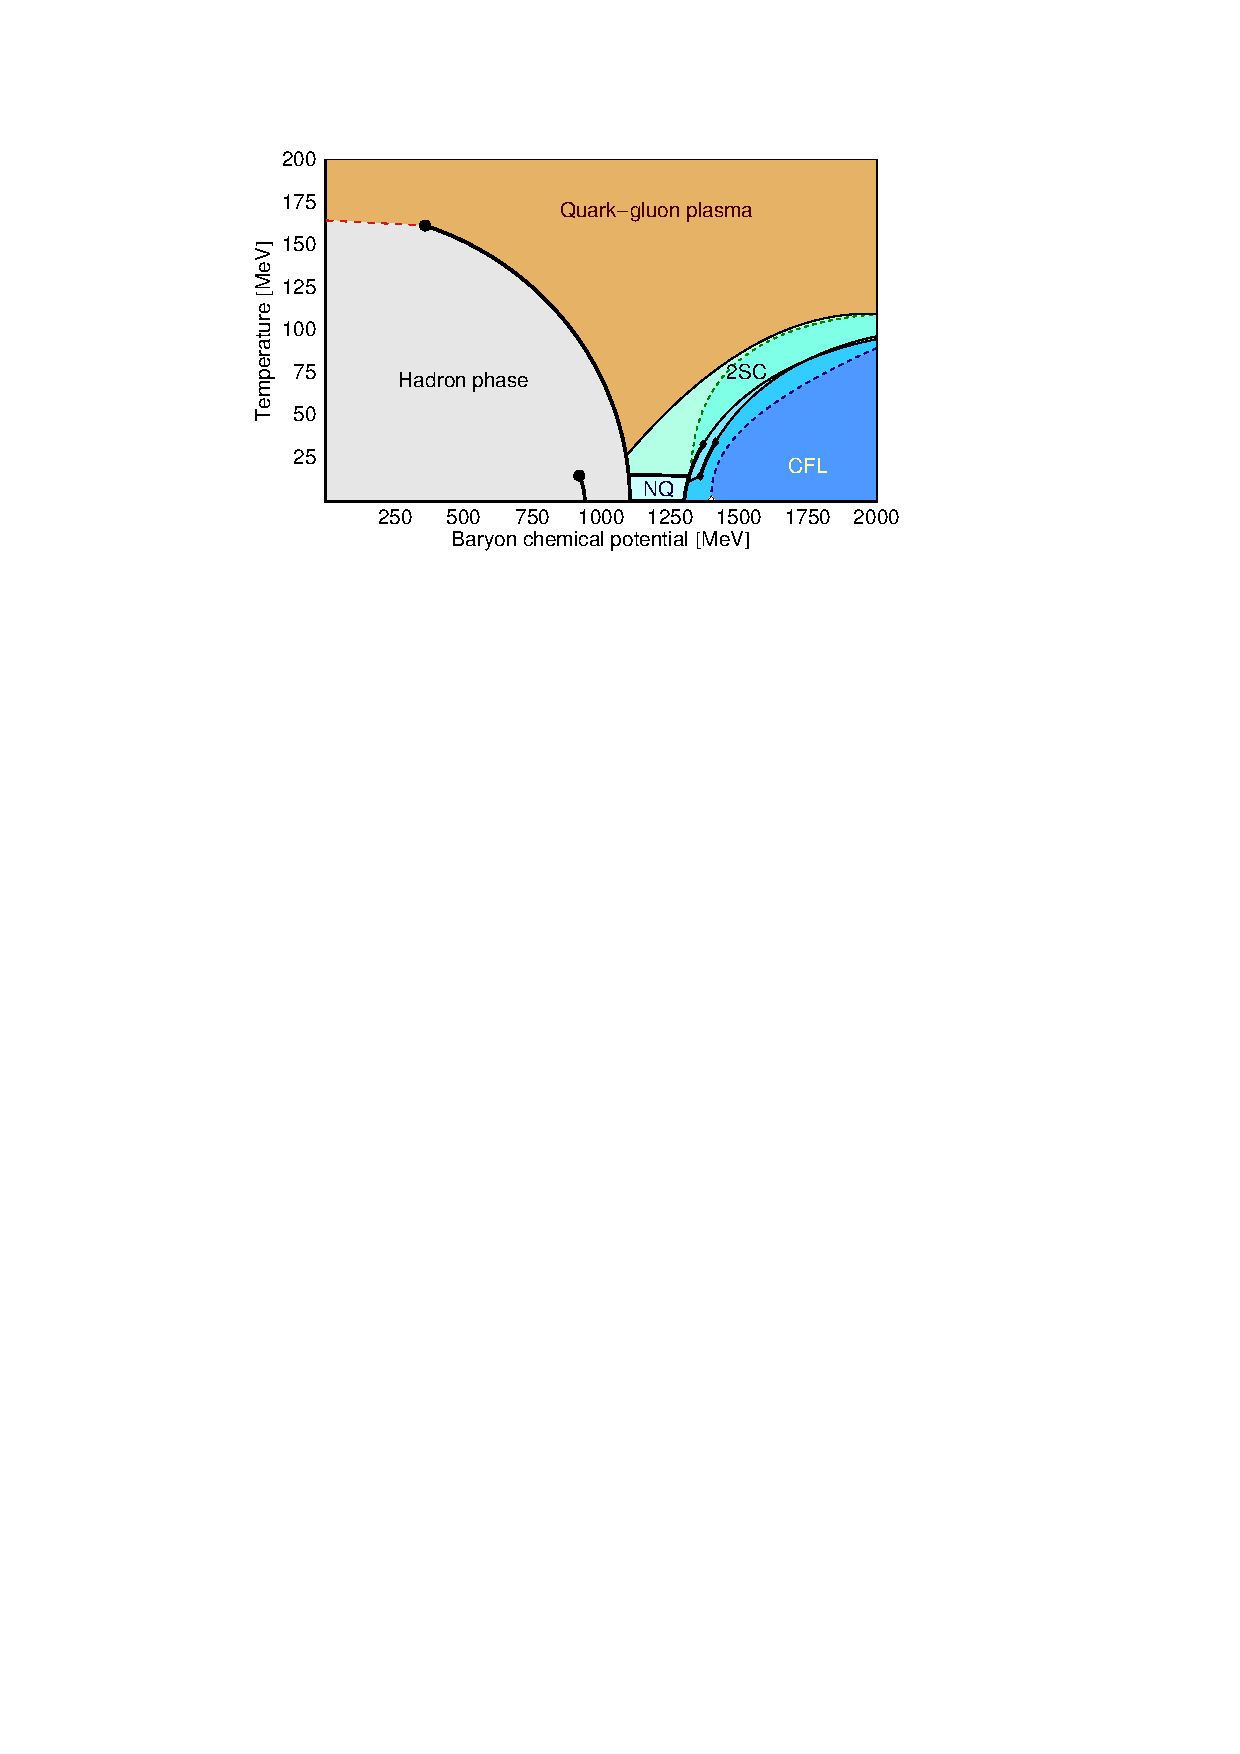
\includegraphics[width=0.45\textwidth]{figures/theory/qcd_phase}
\caption{The QCD phase diagram of nuclear matter as a function of temperature $T$ and baryon chemical potential $\mu$.
The $n\star$ denotes a neutron star.
Figure from Ref.~\cite{Kronfeld:2012uk}.}
\label{fig:qcd_phase}
\end{center}
\end{figure}


\subsection{The Glauber Model}
The basic parameters of a heavy ion collision such as the number of participants \Npart\ and number of binary collisions \Ncoll\ can be determined using the Glauber Monte Carlo simulations \cite{glauberArticle}.
This technique considers a nucleus-nucleus collision as a collection of independent binary nucleon-nucleon collisions; the colliding nuclei are modeled as a set of uncorrelated nucleons being positioned within the nucleus based on a the nuclear density function uniform in azimuthal and in polar angles.
The nuclear density function in this model is a Woods-Saxon distribution given by: 

\begin{align}
\rho(r) = \rho_0 \frac{1 + w (r/R)^2}{1+e^{\frac{r-R}{a}}}
\end{align}
where $\rho_0$ is the nucleon density, $R$ is the nuclear radius, $a$ is the skin depth, $w$ corresponds to deviations from a circular shape and is typically zero for larger nuclei like Cu, W, Au, Pb, and U.
For the Pb nuclei used at the LHC, $w = 0$, $R = 6.62$ fm and $a =0.55$ fm \cite{DEVRIES1987495}.
The nuclear density distribution for Au and Cu is shown in Figure~\ref{fig:nuclearDensity}.

\begin{figure}[htbp]
\begin{center}
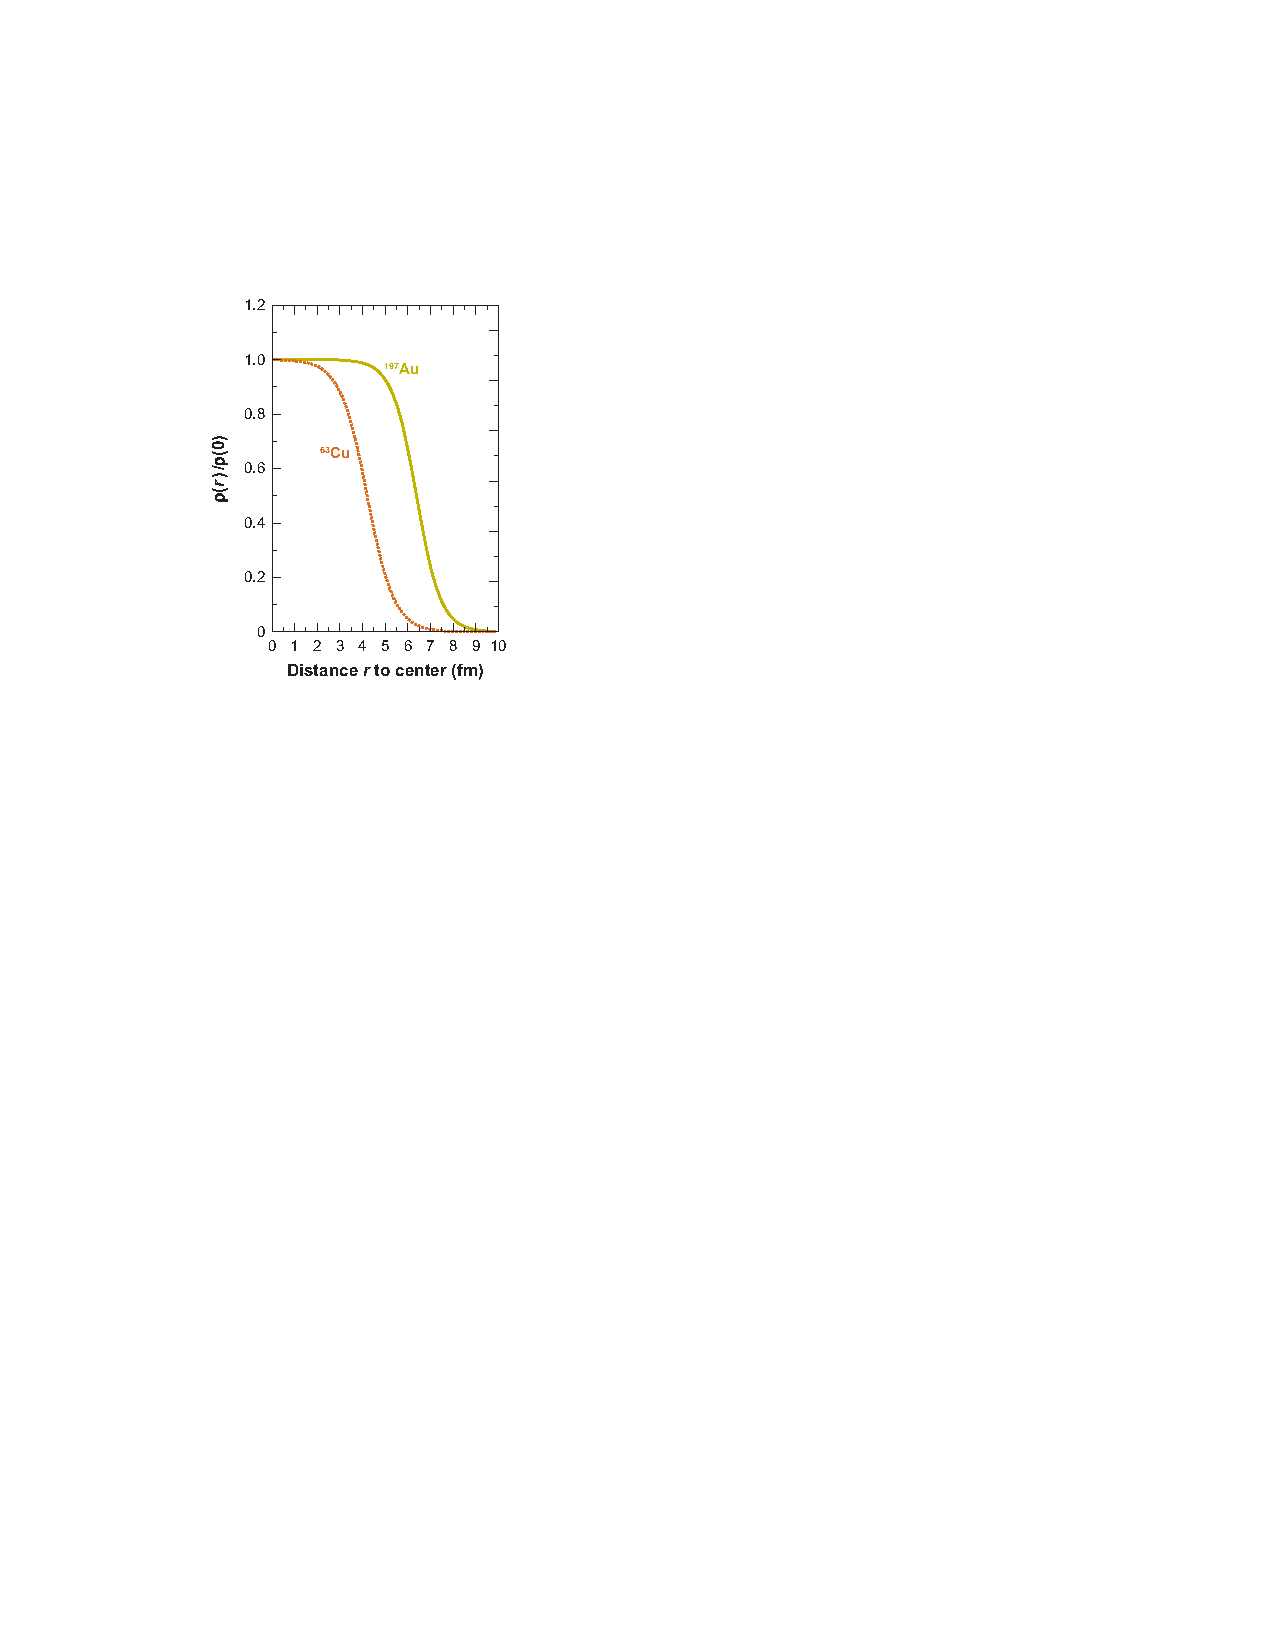
\includegraphics[width=0.35\textwidth]{figures/theory/nuclearDensity}
\caption{ The nuclear density distributions for nuclei used at RHIC: Cu ($w = 0$, $R = 4.2$ fm and $a =0.48$ fm)  and Au ($w = 0$, $R = 6.38$ fm and $a =0.535$ fm) \cite{DEVRIES1987495}.
Figure from Ref.~\cite{doi:10.1146/annurev.nucl.57.090506.123020}.}
\label{fig:nuclearDensity}
\end{center}
\end{figure}

They are then arranged with a random impact parameter $b$ based on the distribution $d\sigma/d b = 2\pi b$ and projected onto the $x-y$ plane as shown in Figure~\ref{fig:glauberMC}.
They are then made to travel on straight trajectories, colliding if $d \leq \sqrt{\sigma_{\mathrm{inel}}^{\mathrm{NN}}/ \pi}$, where $d$ is the distance between the nucleons in a plane transverse to the beam axis and $\sigma_{\mathrm{inel}}^{\mathrm{NN}}$ is the inelastic scattering cross section \cite{doi:10.1146/annurev.nucl.57.090506.123020, Alver:2008aq}.


\begin{figure}[htbp]
\begin{center}
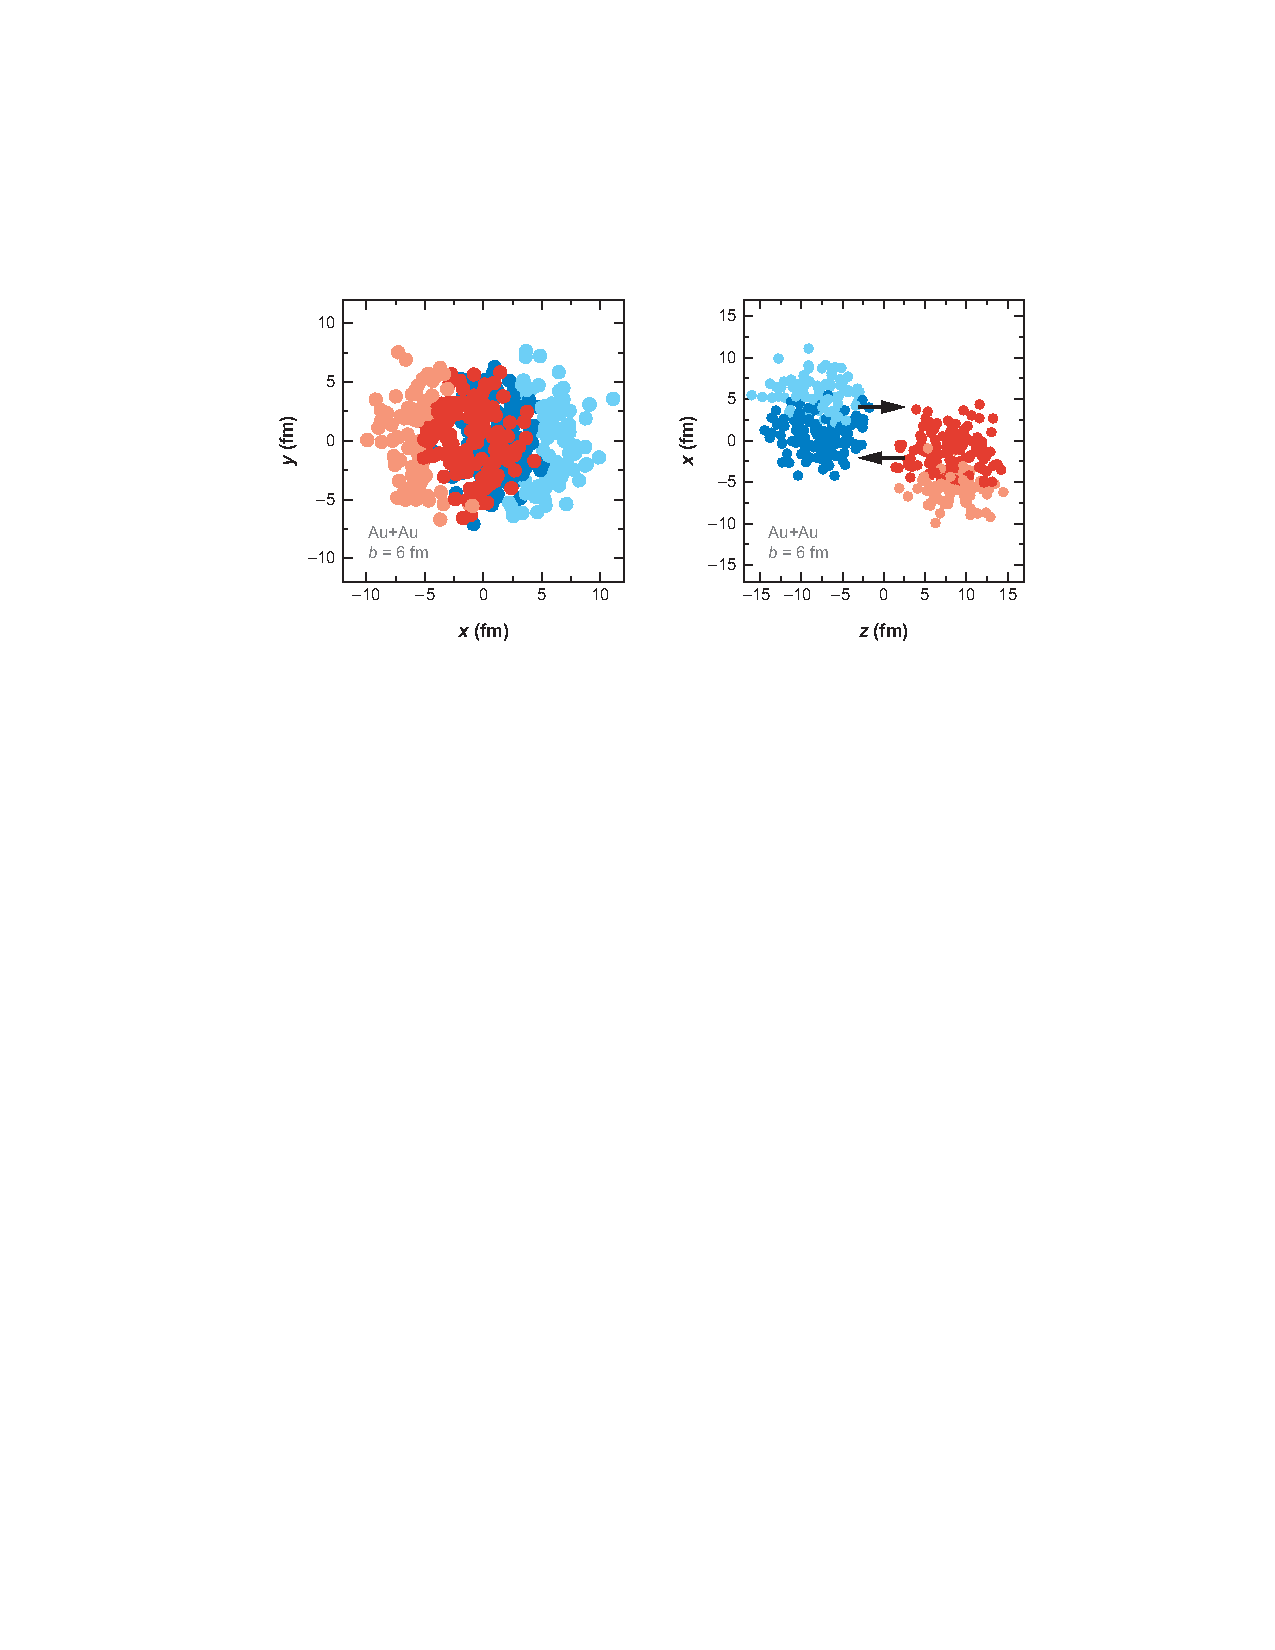
\includegraphics[width=0.85\textwidth]{figures/theory/glauberMC}
\caption{A Glauber Monte Carlo event for $Au+Au$ at \sqrtsnn = 200 geV with impact parameter of 6 fm viewed in the (left) transverse plane and (right) along the beam axis.
Darker circles represent the participating nucleons.
Figure from Ref.~\cite{doi:10.1146/annurev.nucl.57.090506.123020}.}
\label{fig:glauberMC}
\end{center}
\end{figure}

An important parameter for colliding nuclei A and B with $A$ and $B$ nucleons is the thickness function $T_{AB}$.
It describes the effective overlap area in which specific nucleons in the two colliding nuclei can interact.
It can be defined in terms of the probability per unit area of a given nucleon being located at a particular distance $s$ within the nucleus.
For the colliding nuclei $A$ and $B$, this is given by $T_{A}({\bf{s}}) = \int \rho_A ({\bf{s}}, z_A) dz_{A}$ and $T_{B}({\bf{s}}) = \int \rho_B ({\bf{s}}, z_B) dz_{B}$.
Then, $T_{AB}$ is given by

\begin{align}
T_{AB}({\bf b}) = \int T_{A} ({\bf s}) T_{B} ({\bf s-\bf b}) d^2 s
\end{align}
The probability of then having $n$ interactions between nuclei $A$ and $B$ is given by the binomial distribution:

\begin{align}
P(n, { \bf b}) = {{AB} \choose {n}} \Big[T_{AB}( {\bf b} ) \sigma_{\mathrm{inel}}^{\mathrm{NN}} \Big]^n \Big[ 1 - T_{AB}( {\bf b} ) \sigma_{\mathrm{inel}}^{\mathrm{NN}} \Big]^{AB-n}
\end{align}
where the first term is the number of combinations for finding $n$ collisions from $AB$ possibilities, the second term is the probability for having exactly $n$ collisions, and the last term the probability of $AB-n$ misses.
Then the total probability of an interaction between A and B is:

\begin{align}
\frac{d^2  \sigma_{\mathrm{inel}}^{\mathrm{AB}} }{db^2} \equiv p_{\mathrm{inel}}^{\mathrm{AB}} (b) = \sum_{n=1}^{AB} P(n, {\bf b}) = 1- \Big[ 1 - T_{AB}( {\bf b} ) \sigma_{\mathrm{inel}}^{\mathrm{NN}} \Big]^{AB}
\end{align}
and the total cross section is given by

\begin{align}
\sigma_{\mathrm{inel}}^{\mathrm{AB}} = \int_0^\infty 2\pi b db \Bigg[ 1- \Big( 1 - T_{AB}( {\bf b} ) \sigma_{\mathrm{inel}}^{\mathrm{NN}}  \Big)^{AB} \Bigg]
\end{align}
and \Ncoll\ and \Npart are given by \cite{Kharzeev:2000ph, Bialas:1976ed}:

\begin{align}
\Ncoll (b) = & \sum_{n=1}^{AB} n P(n, b) =  AB \times T_{AB}(b) \sigmainel \\
\Npart (b) = & A \int T_A ({\bf s}) \Big[ 1 - \big(1-T_B ({\bf s - b}) \sigmainel \big)^B \Big] d^2 s \\
+ & B \int T_B ({\bf s-b}) \Big[ 1 - \big(1-T_A ({\bf s}) \sigmainel \big)^A \Big] d^2 s \nonumber
\end{align}
The correlation between \Ncoll\ and \Npart\ can be seen in Figure~\ref{fig:NcollNpart}.
The charged particle multiplicity $N_{\mathrm{ch}}$ along with the combination of \Npart\ and impact parameter $b$ can be used to determine the centrality of a heavy ion event.
An example of this is shown in Figure~\ref{fig:cent_estimate}.

\begin{figure}
\begin{center}
  \begin{minipage}[b]{0.4\textwidth}
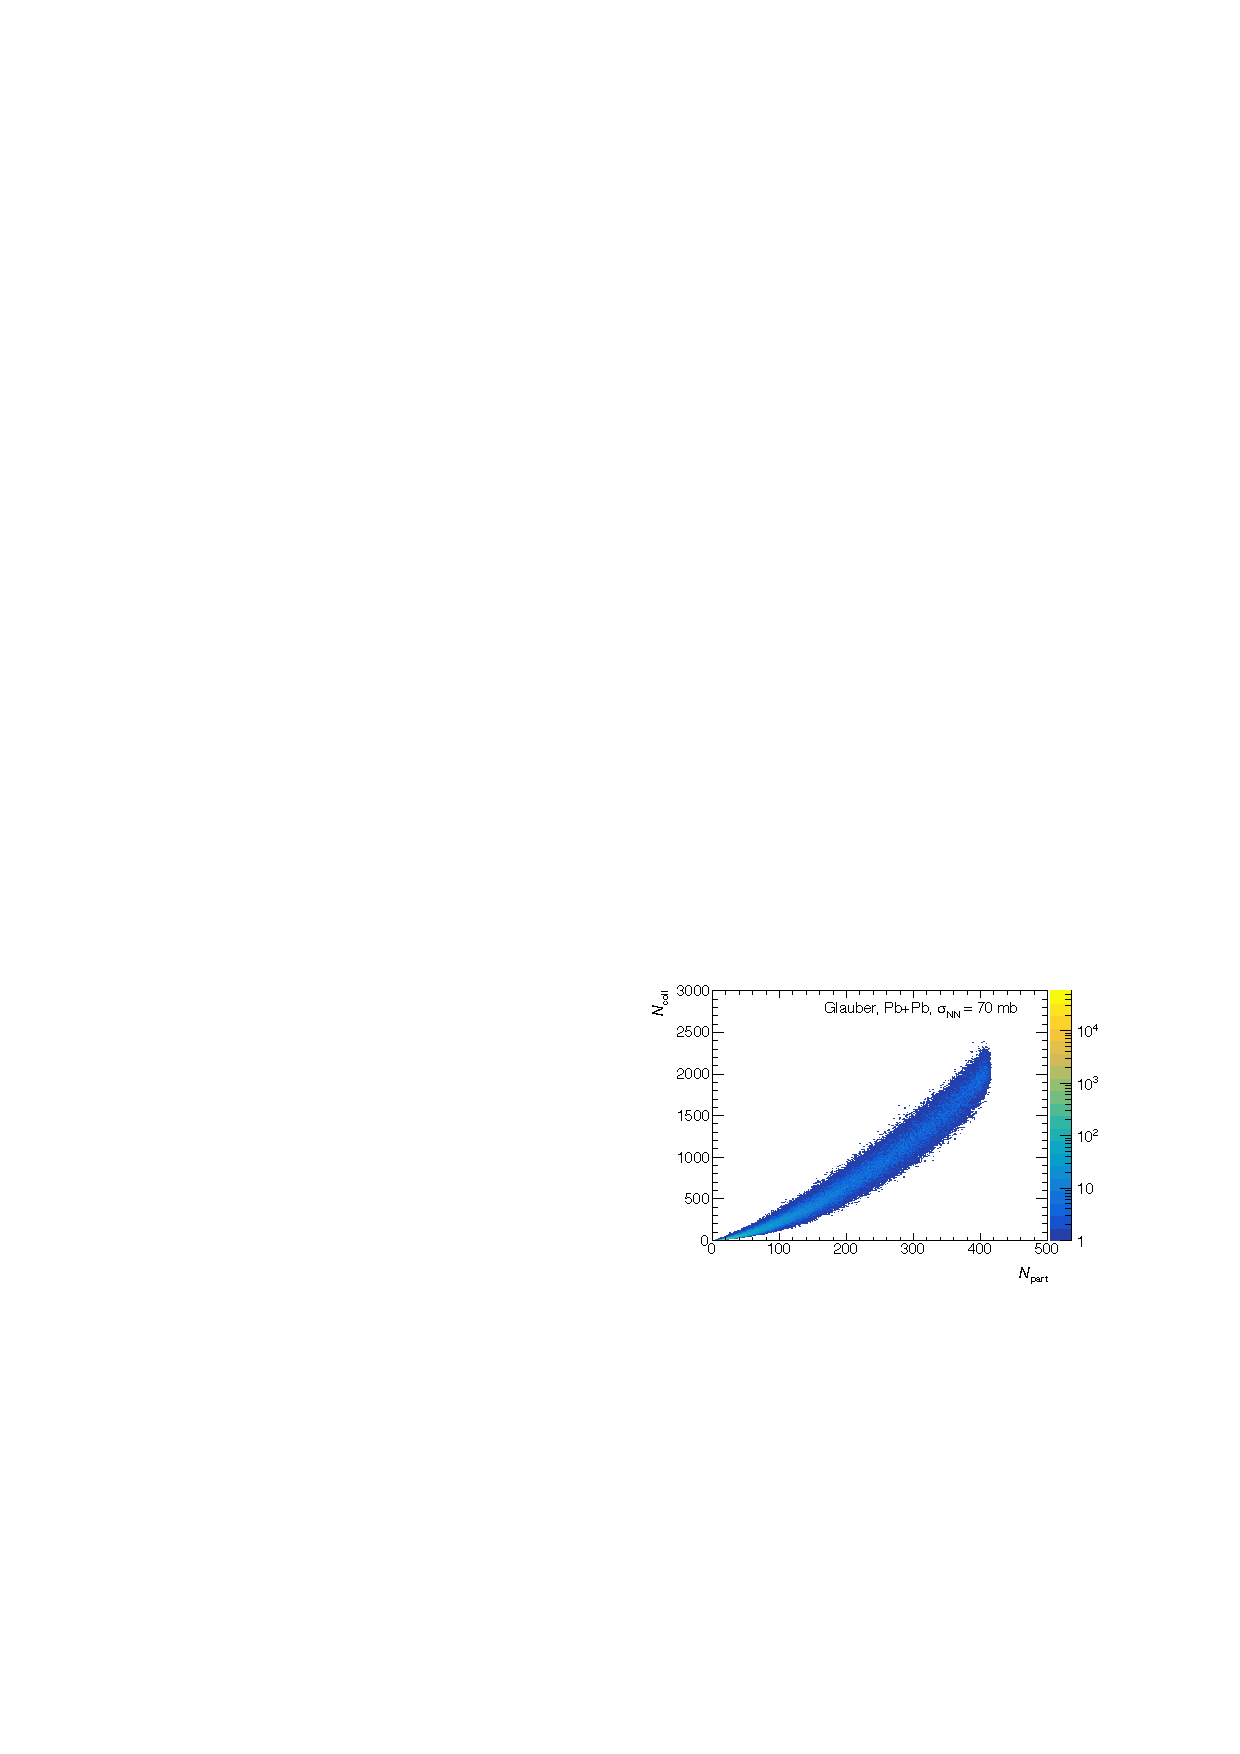
\includegraphics[width=\textwidth]{figures/theory/NcollNpart}
\caption{The $\Ncoll-\Npart$ correlation for \pbpb\ collisions at \sqrtsnn\ = 5.02 TeV.
Figure from Ref.~\cite{Perepelitsa:2212936}.}
\label{fig:NcollNpart}
  \end{minipage}
 \qquad  \qquad  \qquad
  \begin{minipage}[b]{0.4\textwidth}
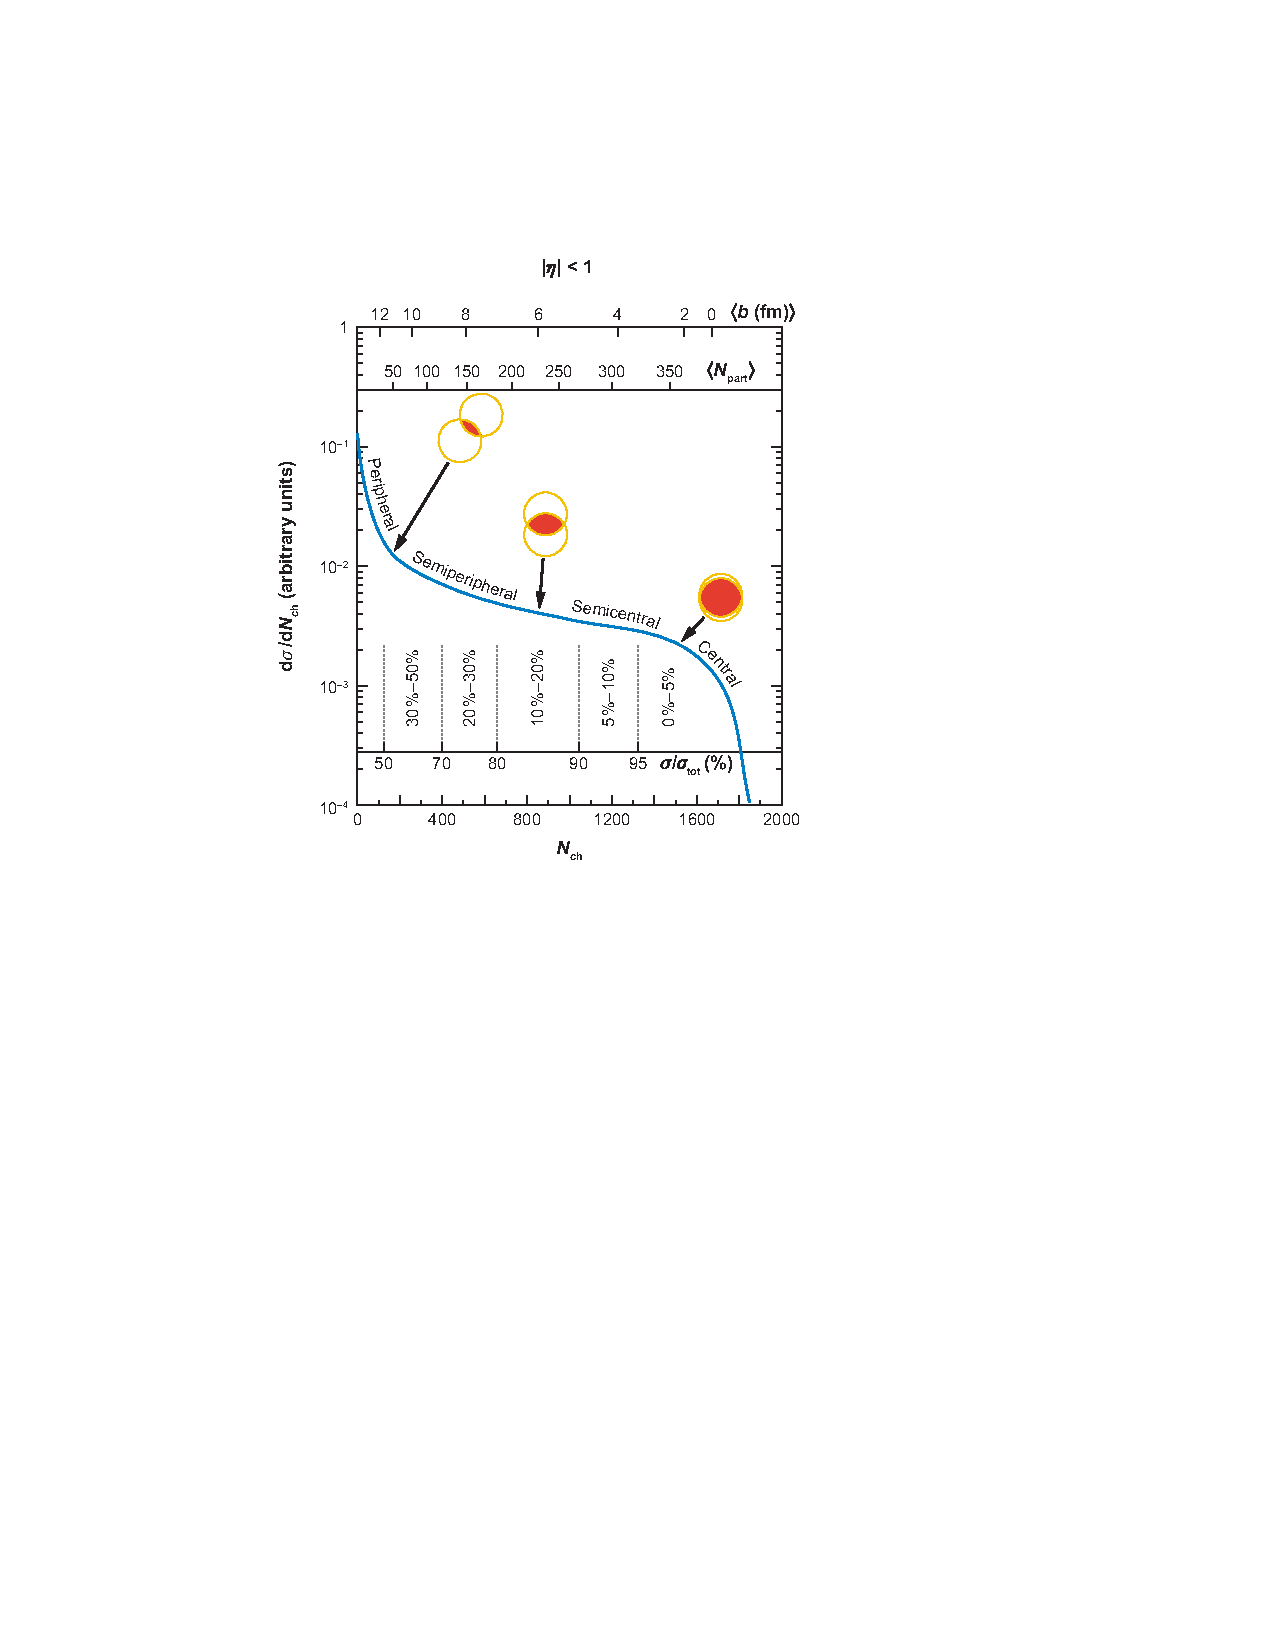
\includegraphics[width=\textwidth]{figures/theory/cent_estimate}
\caption{The correlation between the observable \Nch\ and \Npart\ to determine the centrality distribution.
Figure from Ref.~\cite{doi:10.1146/annurev.nucl.57.090506.123020}.}
\label{fig:cent_estimate}
  \end{minipage}
  \end{center}
\end{figure}





%Hydrodynamic models of photon emission can be used to describe data measured at both RHIC \cite{PhysRevLett.104.132301} and LHC \cite{2016235} energies and suggest that the initial temperature of the QGP is 300--600 MeV \cite{PhysRevC.81.034911}.
%Each nucleus contains many colored quarks and antiquarks, with three more quarks than anti-quarks per nucleon, with the $q\bar{q}$ popping in and out of the vacuum due to quantum fluctuations.
%These $q\bar{q}$ pairs are sources of transverse color fields and the corresponding force carriers, the gluons.
%Lattice QCD calculations in these regions show that the transition between a hadronic gas and the QGP occurs at a temperature of approximately 160 MeV and corresponds to an energy density of 0.5 GeV/fm$^3$ \cite{Borsanyi:2010bp}.
%Heavy ion collisions are a tool that can be used as a tool to study the quark-gluon plasma (QGP) \cite{SHURYAK198071}.

%\section{Heavy Ion Collisions}
%\label{sec:HICollisions}
%% !TEX root = thesis-ex.tex
Heavy ion collisions can be used as a tool to study the Quark Gluon Plasma \cite{SHURYAK198071} . They provide access to the otherwise confined partons, and give insight into the QCD phase diagram and the transition between the QGP and hadronic matter. 

In a heavy ion collision, the colliding nuclei are accelerated to relativistic energies and are Lorentz contracted discs. In the case of a \pbpb\ collision the relativistic $\gamma$ factor is between 100 and 2500 for beam rapidities of $y = 5.3$ and 8.5. Each nucleus contains many colored quarks and antiquarks, with three more quarks than anti-quarks per nucleon, with the $q\bar{q}$ popping in and out of the vacuum due to quantum fluctuations. These $q\bar{q}$ pairs are sources of transverse color fields and the corresponding force carriers, the gluons. 

When these pancake like discs collide, their color fields interact and there is a color charge exchange, producing longitudinal color fields that fill the space between the receding discs. While the maximum energy density in the process occurs just at the collision, the energy density 1 fm/c after the collision is 12 $\mathrm{GeV} / \mathrm{fm}^3$, much higher than the 500 $\mathrm{MeV} / \mathrm{fm}^3$ in a typical hadron. Lattice QCD calculations in thermodynamics show that at these energies, the partons produced in the collision cannot be treated as a collection of distinct hadrons. 
%In fact, these partons are strongly coupled to each other and form a medium called the Quark Gluon Plasma (QGP) \cite{???}. 

%In a heavy ion collision, the experimenter can only tune the size of the colliding nuclei, and the energy that they are being collided at. There is no experimental control over the impact parameter or the structure functions that dictate the momentum distribution of nucleons within the nucleus. These have to be determined event by

% most of the partons are participate in soft interactions that do not involve large transverse momentum transfer, and are hence scattered only at small angles. A small fraction of the colliding partons however do undergo hard perturbative interactions and lead to particles with large transverse momenta.
%These subsequently decaying to $q\bar{q}$ pairs. 
%The QGP can be described by relativistic hydrodynamics, and has a viscosity to entropy ratio that is almost at the theoretical minimum of of $\eta / S = 1/4\pi$ \cite{5,6, check126}. 

After the collision the energy density between the receding nuclei starts to decrease as the QGP cools and expands. This process, seen in Figure~\ref{fig:qgp_form}, continues till the energy density drops to below that within a hadron and the fluid ``hadronizes''. These individual hadrons briefly scatter off of each other before they freely fly towards the detector (freeze-out).

%Once formed, the QGP flows hydrodynamically, with the initial pressure driving the expansion and the subsequent cooling. 
% It is to be noted that there is QGP continuously formed in the wake of the nuclei since the partons produced at large rapidities are highly relativistic and 

\begin{figure}[htbp]
\begin{center}
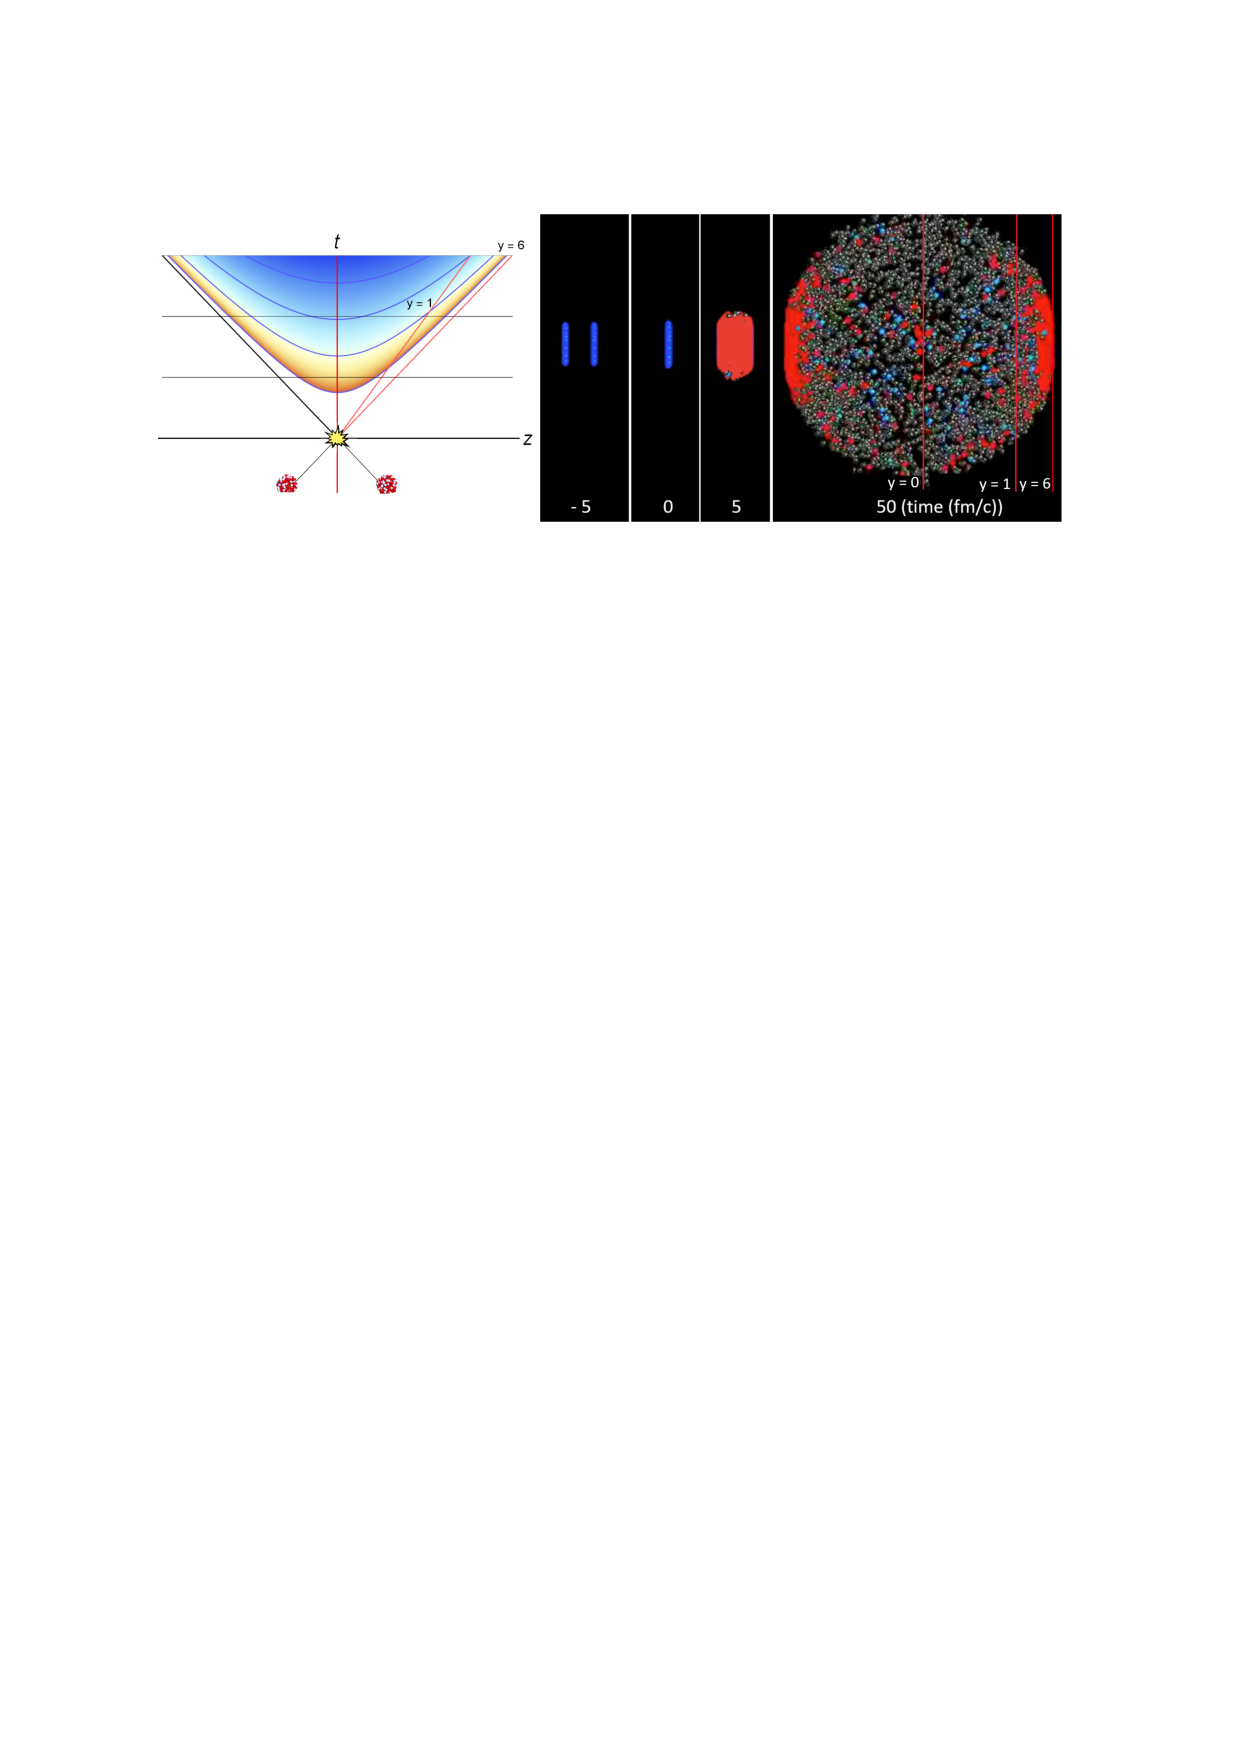
\includegraphics[width=0.85\textwidth]{figures/theory/qgp_formation}
\caption{(left) Space-time diagram for a heavy ion collision. The color is indicative of the temperature of the QGP formed. (right) Snapshots of a heavy ion collision at $\sqrtsnn = 2.76$ TeV at different times. The Lorentz contracted nuclei are in blue while the QGP is in red. Figure from Reference \cite{Busza:2018rrf}.  }
\label{fig:qgp_form}
\end{center}
\end{figure}

While Figure~\ref{fig:qgp_form} shows snapshots of a head on (central) collision between two large nuclei, it is possible to have collisions where the impact parameter is larger and hence the overlap region is smaller. These collisions, called peripheral collisions, qualitatively undergo the same process described above, with the size and shape of the QGP being different.

% In fact, peripheral collisions are very similar to proton-proton collisions, with differences coming mainly from nuclear PDFs.

The basic parameters of a heavy ion collision such as the number of participants \Npart\ and number of binary collisions \Ncoll\ can be determined using the Glauber Monte Carlo simulations \cite{glauberArticle, glauberMisc}. This technique considers a nucleus-nucleus collision as a collection of independent binary nucleon-nucleon collisions; the colliding nuclei are modeled as a set of uncorrelated nucleons being positioned within the nucleus based on a the nuclear density function uniform in azimuthal and in polar angles. The nuclear density function shown in Figure~\ref{fig:nuclearDensity} for Au and Cu, is given by:

\begin{align}
\rho(r) = \rho_0 \frac{1 + w (r/R)^2}{1+e^{\frac{r-R}{a}}}
\end{align}
where $\rho_0$ is the nucleon density, $R$ is the nuclear radius, $a$ is the skin depth, $w$ corresponds to deviations from a circular shape and is typically zero for larger nuclei like Cu, W, Au, Pb, and U. For the Pb nuclei used at the LHC, $w = 0$, $R = 6.62$ fm and $a =0.55$ fm \cite{DEVRIES1987495}. 

\begin{figure}[htbp]
\begin{center}
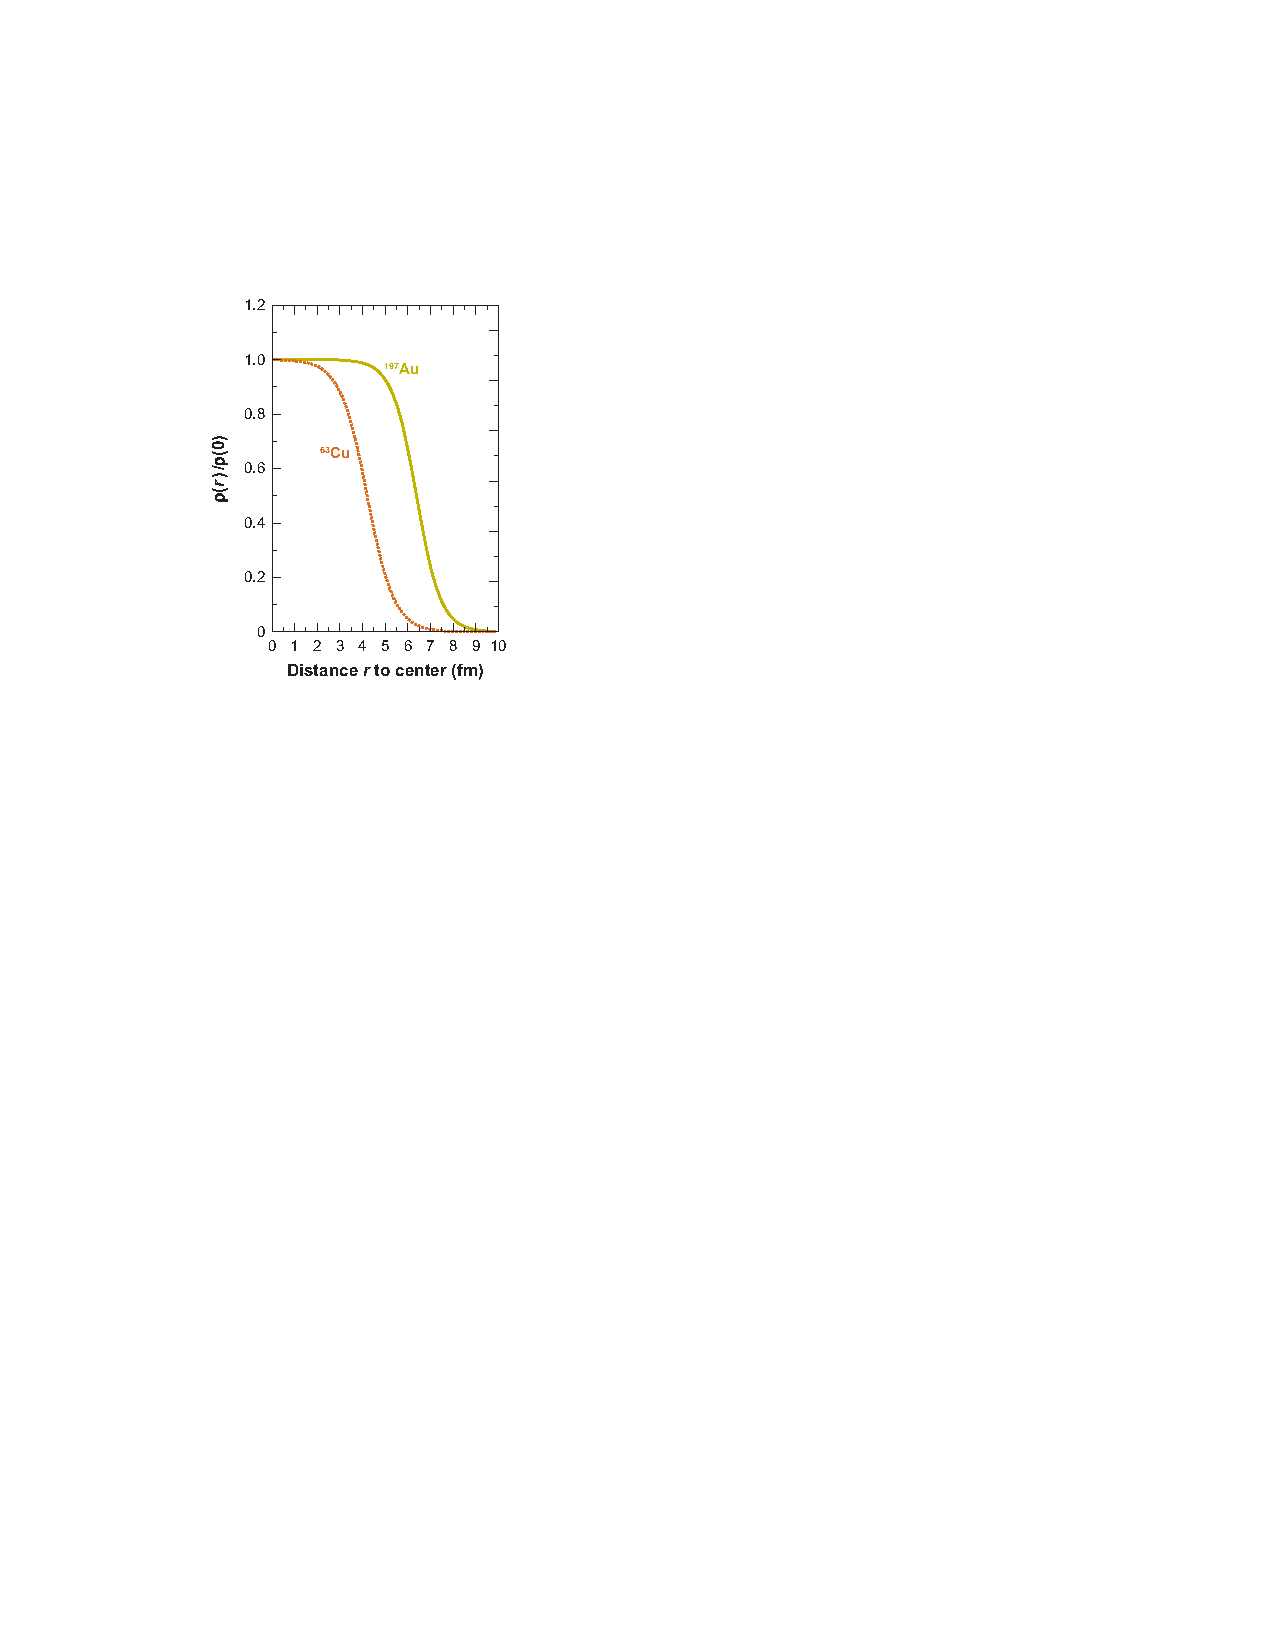
\includegraphics[width=0.45\textwidth]{figures/theory/nuclearDensity}
\caption{ The nuclear density distributions for nuclei used at RHIC: Cu ($w = 0$, $R = 4.2$ fm and $a =0.48$ fm)  and Au ($w = 0$, $R = 6.38$ fm and $a =0.535$ fm) \cite{doi:10.1146/annurev.nucl.57.090506.123020, DEVRIES1987495}.}
\label{fig:nuclearDensity}
\end{center}
\end{figure}

They are then arranged with a random impact parameter $b$ based on the distribution $d\sigma/d b = 2\pi b$ and projected onto the $x-y$ plane as shown in Figure~\ref{fig:glauberMC}. They are then made to travel on straight trajectories, colliding if $d \leq \sqrt{\sigma_{\mathrm{inel}}^{\mathrm{NN}}/ \pi}$, where $d$ is the distance between the nucleons in a plane transverse to the beam axis and $\sigma_{\mathrm{inel}}^{\mathrm{NN}}$ is the inelastic scattering cross section. \cite{doi:10.1146/annurev.nucl.57.090506.123020, Alver:2008aq}

\begin{figure}[htbp]
\begin{center}
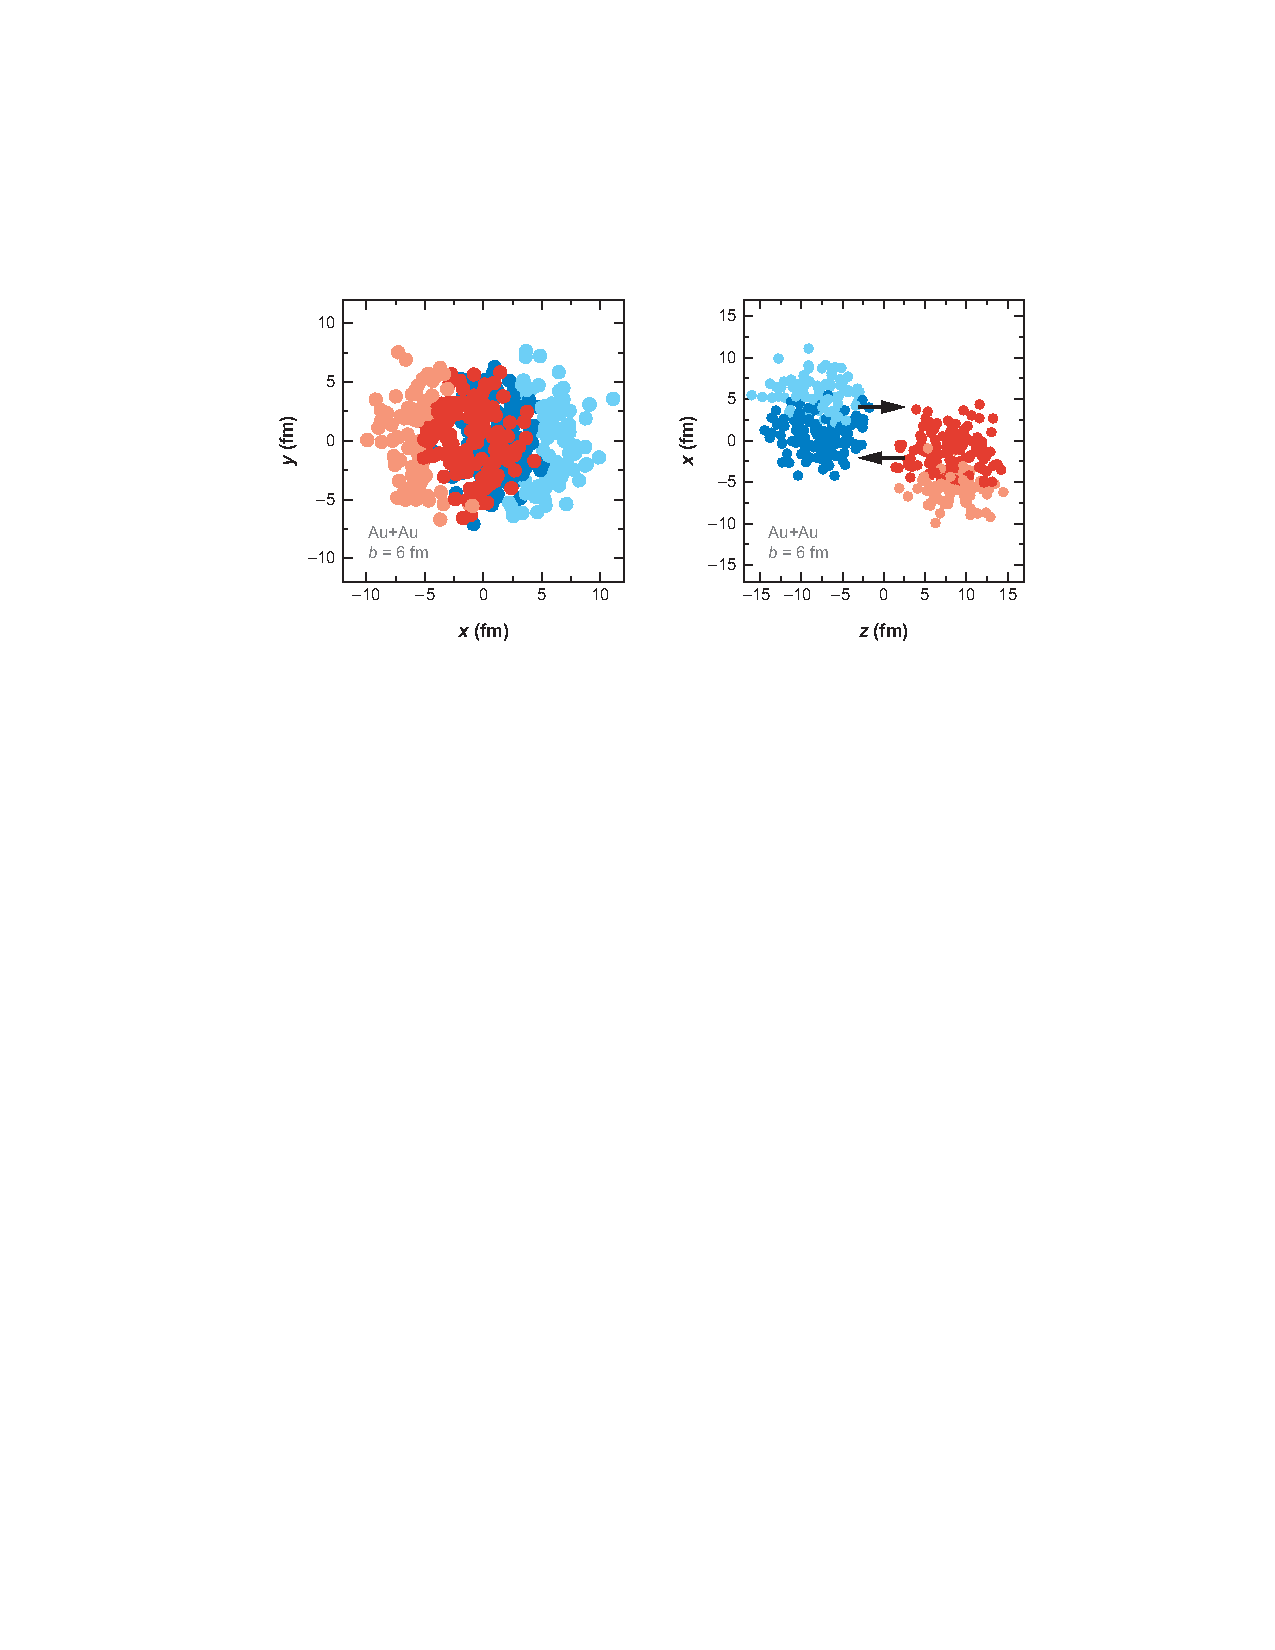
\includegraphics[width=0.85\textwidth]{figures/theory/glauberMC}
\caption{A Glauber Monte Carlo event for $Au+Au$ at \sqrtsnn = 200 geV with impact parameter of 6 fm viewed in the (left) transverse plane and (right) along the beam axis. Darker circles represent the participating nucleons. Taken from \cite{doi:10.1146/annurev.nucl.57.090506.123020}. }
\label{fig:glauberMC}
\end{center}
\end{figure}



An important parameter for colliding nuclei A and B with $A$ and $B$ nucleons is the thickness function $T_{AB}$. It describes the effective overlap area in which specific nucleons in the two colliding nuclei can interact. It can be defined in terms of the probability per unit area of a given nucleon being located at a particular distance $s$ within the nucleus. For the colliding nuclei $A$ and $B$, this is given by $T_{A}({\bf{s}}) = \int \rho_A ({\bf{s}}, z_A) dz_{A}$ and $T_{B}({\bf{s}}) = \int \rho_B ({\bf{s}}, z_B) dz_{B}$. Then, $T_{AB}$ is given by

\begin{align}
T_{AB}({\bf b}) = \int T_{A} ({\bf s}) T_{B} ({\bf s-\bf b}) d^2 s
\end{align}

The probability of then having $n$ interactions between nuclei $A$ and $B$ is given by the binomial distribution:

\begin{align}
P(n, { \bf b}) = {{AB} \choose {n}} \Big[T_{AB}( {\bf b} ) \sigma_{\mathrm{inel}}^{\mathrm{NN}} \Big]^n \Big[ 1 - T_{AB}( {\bf b} ) \sigma_{\mathrm{inel}}^{\mathrm{NN}} \Big]^{AB-n}
\end{align}

where the first term is the number of combinations for finding $n$ collisions from $AB$ possibilities, the second term is the probability for having exactly $n$ collisions, and the last term the probability of $AB-n$ misses. Then the total probability of an interaction between A and B is 

%\frac{d^2  s\sigma_{\mathrm{inel}}^{\mathrm{AB}} } {d b^2}  \def % p p_{\mathrm{inel}^{AB} (b) = \sum_{n=1}^{AB} P(n, {\bf b}) = %1- \Big[ 1 - T_{AB}( {\bf b} ) \sigma_{\mathrm{inel}}^{\mathrm{NN}} \Big]^{AB-n}

\begin{align}
\frac{d^2  \sigma_{\mathrm{inel}}^{\mathrm{AB}} }{db^2} \equiv p_{\mathrm{inel}}^{\mathrm{AB}} (b) = \sum_{n=1}^{AB} P(n, {\bf b}) = 1- \Big[ 1 - T_{AB}( {\bf b} ) \sigma_{\mathrm{inel}}^{\mathrm{NN}} \Big]^{AB}
\end{align}

Then the total cross section is given by

\begin{align}
\sigma_{\mathrm{inel}}^{\mathrm{AB}} = \int_0^\infty 2\pi b db \Bigg[ 1- \Big( 1 - T_{AB}( {\bf b} ) \sigma_{\mathrm{inel}}^{\mathrm{NN}}  \Big)^{AB} \Bigg]
\end{align}

and \Ncoll\ and \Npart are given by \cite{Kharzeev:2000ph, Bialas:1976ed}

\begin{align}
\Ncoll (b) = & \sum_{n=1}^{AB} n P(n, b) =  AB \times T_{AB}(b) \sigmainel \\
\Npart (b) = & A \int T_A ({\bf s}) \Big[ 1 - \big(1-T_B ({\bf s - b}) \sigmainel \big)^B \Big] d^2 s \\
+ & B \int T_B ({\bf s-b}) \Big[ 1 - \big(1-T_A ({\bf s}) \sigmainel \big)^A \Big] d^2 s \nonumber
\end{align}

The correlation between \Ncoll\ and \Npart\ can be seen in Figure~\ref{fig:NcollNpart}

\begin{figure}[htbp]
\begin{center}
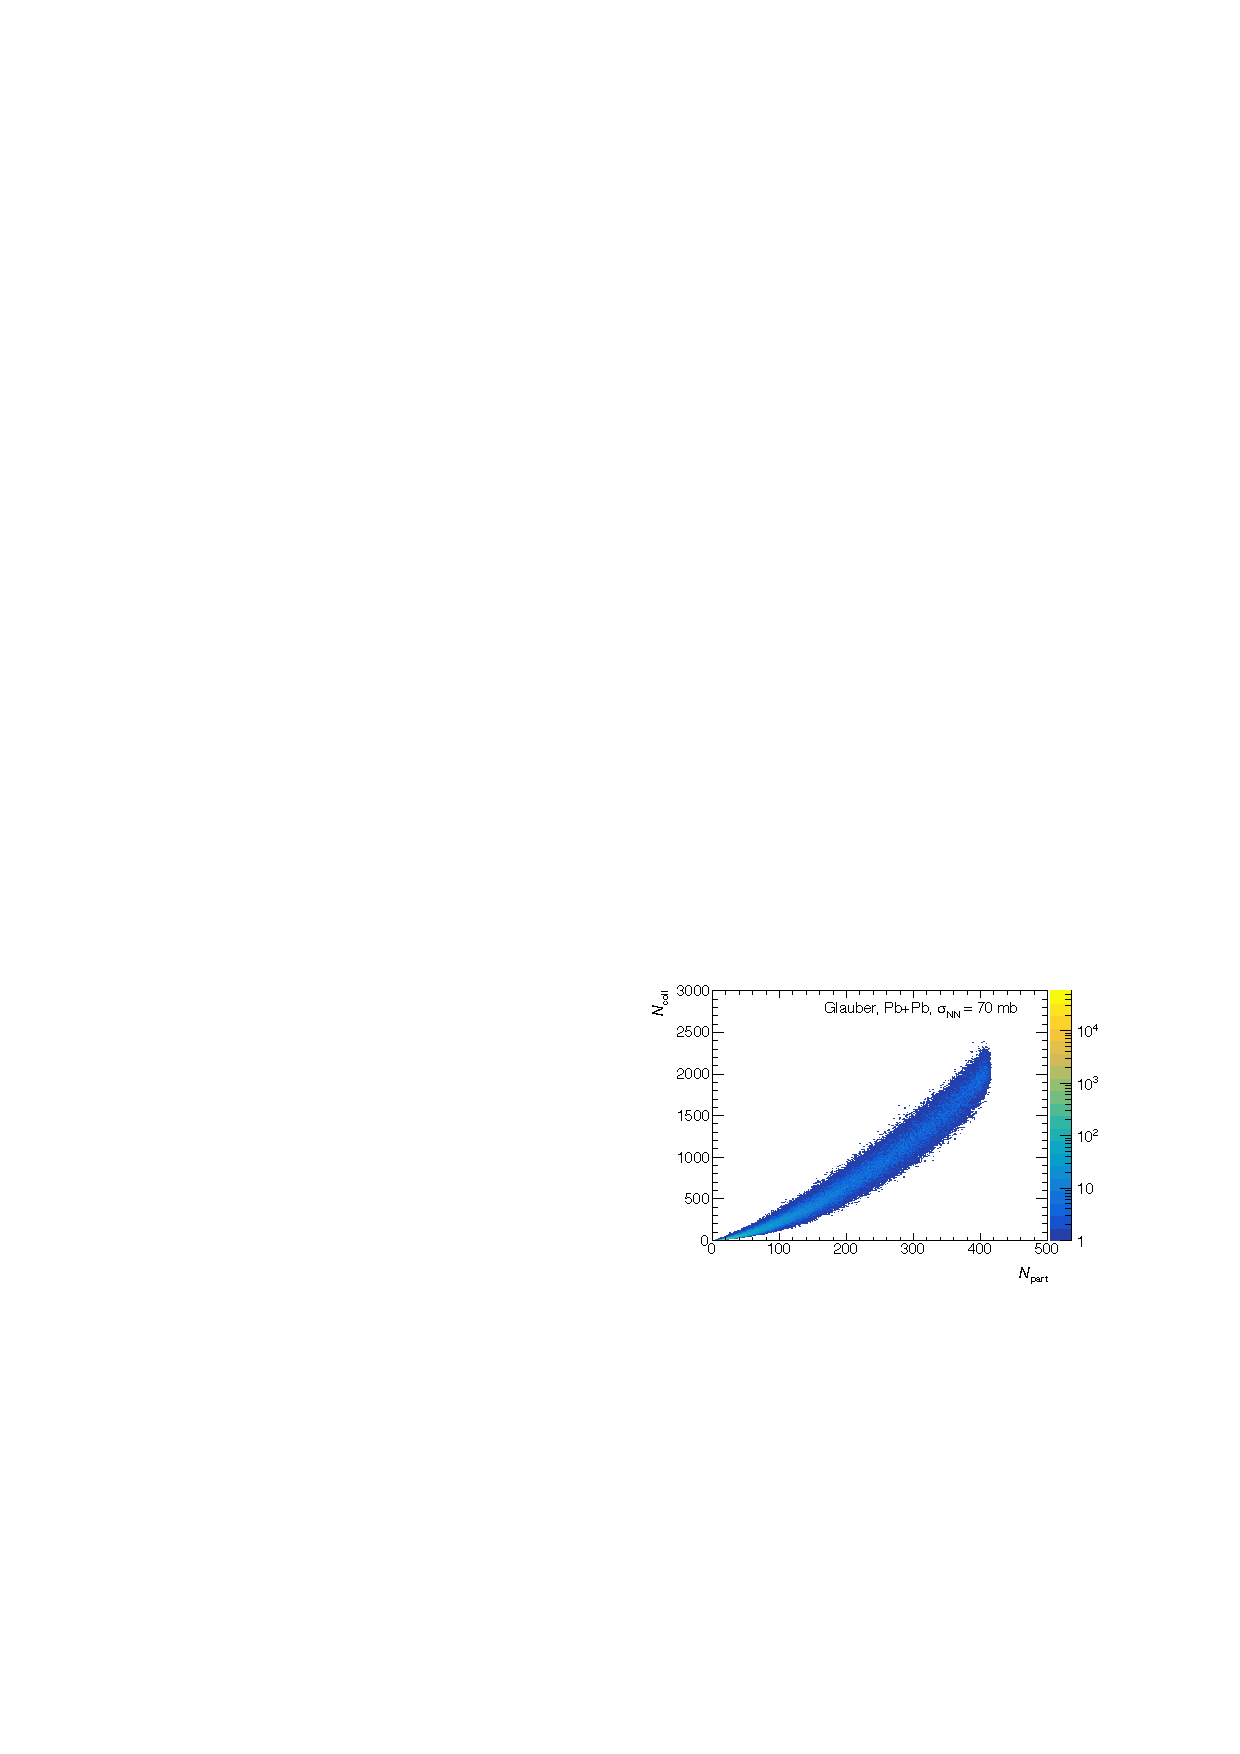
\includegraphics[width=0.55\textwidth]{figures/theory/NcollNpart}
\caption{The $\Ncoll-\Npart$ correlation for \pbpb\ collisions at \sqrtsnn\ = 5.02 TeV. Taken from \cite{Perepelitsa:2212936}. }
\label{fig:NcollNpart}
\end{center}
\end{figure}

The charged particle multiplicity $N_{\mathrm{ch}}$ along with the combination of \Npart\ and impact parameter $b$ can be used to determine the centrality of a heavy ion event. An example of this is shown in Figure~\ref{fig:cent_estimate}.


\begin{figure}[htbp]
\begin{center}
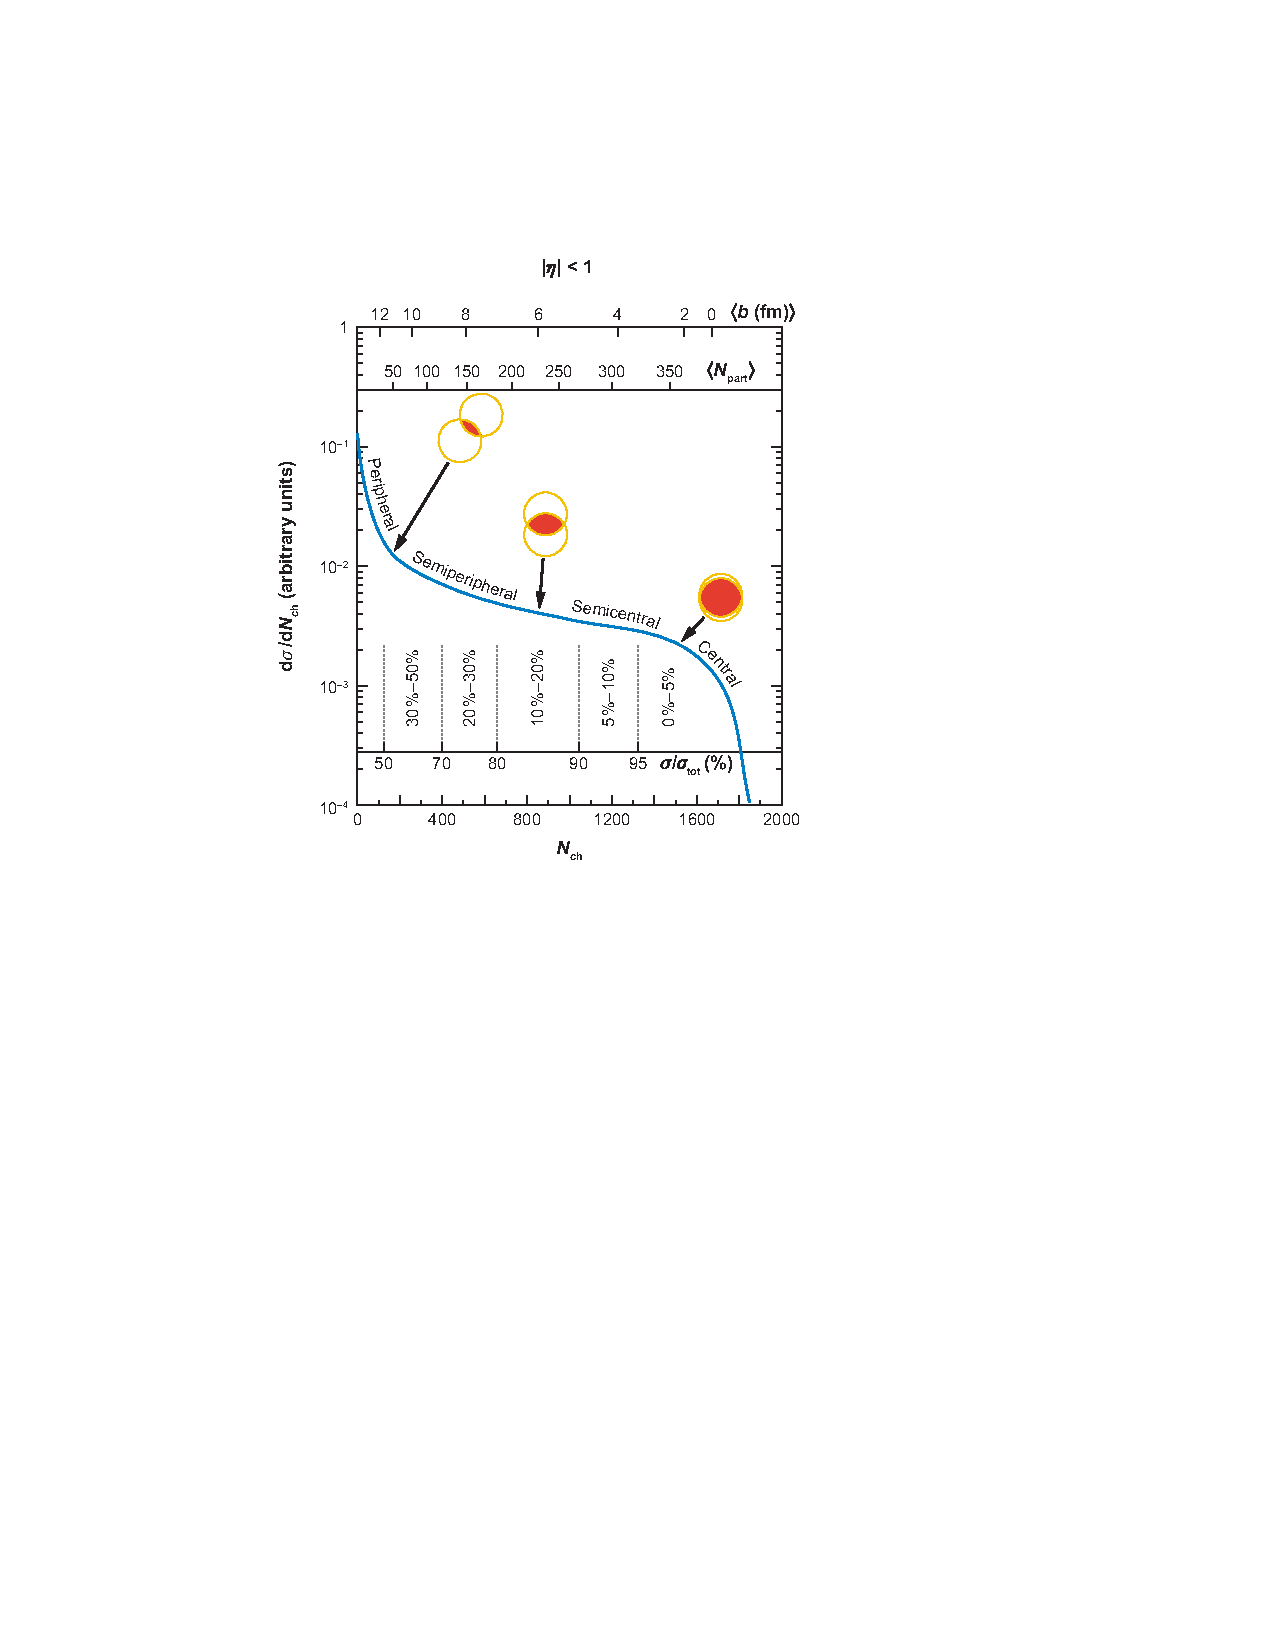
\includegraphics[width=0.45\textwidth]{figures/theory/cent_estimate}
\caption{The correlation between the observable \Nch\ and \Npart\ to determine the centrality distribution. Taken from \cite{doi:10.1146/annurev.nucl.57.090506.123020}. }
\label{fig:cent_estimate}
\end{center}
\end{figure}

%In these collisions, the QGP formed is more lenticular in the transverse direction.
% Of course, the colliding nuclei are not perfectly smooth objects and are made of individual nucleons giving them a non-uniform structure. This results in the energy density in the overlap region being non-uniform with any variations giving rise to pressure gradients that cause azimuthal anisotropies in the momentum distribution of the produced particles. 

%The heavy ion collision system is an extraordinarily useful laboratory to study QCD because it gives access to the otherwise confined partons and provides for a way to study the phase transition between the QGP and ordinary hadronic matter. It is also able to replicate the conditions in the early universe, just after the Big Bang \cite{23, 24}, when it was too hot for hadrons to exist in the form that they do now. 

%We can differentiate different nucleons in the collision as per the following:
%\subparagraph{$\mathrm{N}_{\mathrm{part}}$: } This is the number nucleons that have collided with at least one other nucleon, and can be said to have participated in the heavy ion collision.
%\subparagraph{$\mathrm{N}_{\mathrm{coll}}$: } This is the number of binary collisions that take place between the nucleons of the colliding nuclei. It is typically much larger than \Npart.
%\subparagraph{$\mathrm{N}_{\mathrm{spec}}$: } This is the number nucleons that do not encounter any nucleon from the other nucleus and are just spectators to the collision. 

%The properties of the QGP can be determined by azimuthal correlation measurements \cite{5, 6, 90}, while how it interacts with a high energy parton can be determined by jet studies \cite{91, 92, 69, etc}. 


%%%%%%%%%%%%%%%%%%%%%%%%%%%%%%%%%%%%%%%%%%%%%%%%%%%%%%%%%%%%%%%%%%%%%%%%%




\section{Jets and Jet Quenching}
\label{sec:jets}
% !TEX root = thesis-ex.tex


Hard scatterings in particle collisions result in the production of highly energetic partons that form conical sprays of hadrons called jets. A schematic of this process is shown in Figure~\ref{fig:feynman_jet}. Jet production in a vacuum is well described in context of perturbative QCD \cite{Sjostrand:2007gs} where processes involving large momentum transfers like high \pt\ hadron production can be described in terms of the parton distribution functions, scattering cross sections, and final state fragmentation functions as shown below \cite{Qin:2015srf}:


\begin{figure}[htbp]
\begin{center}
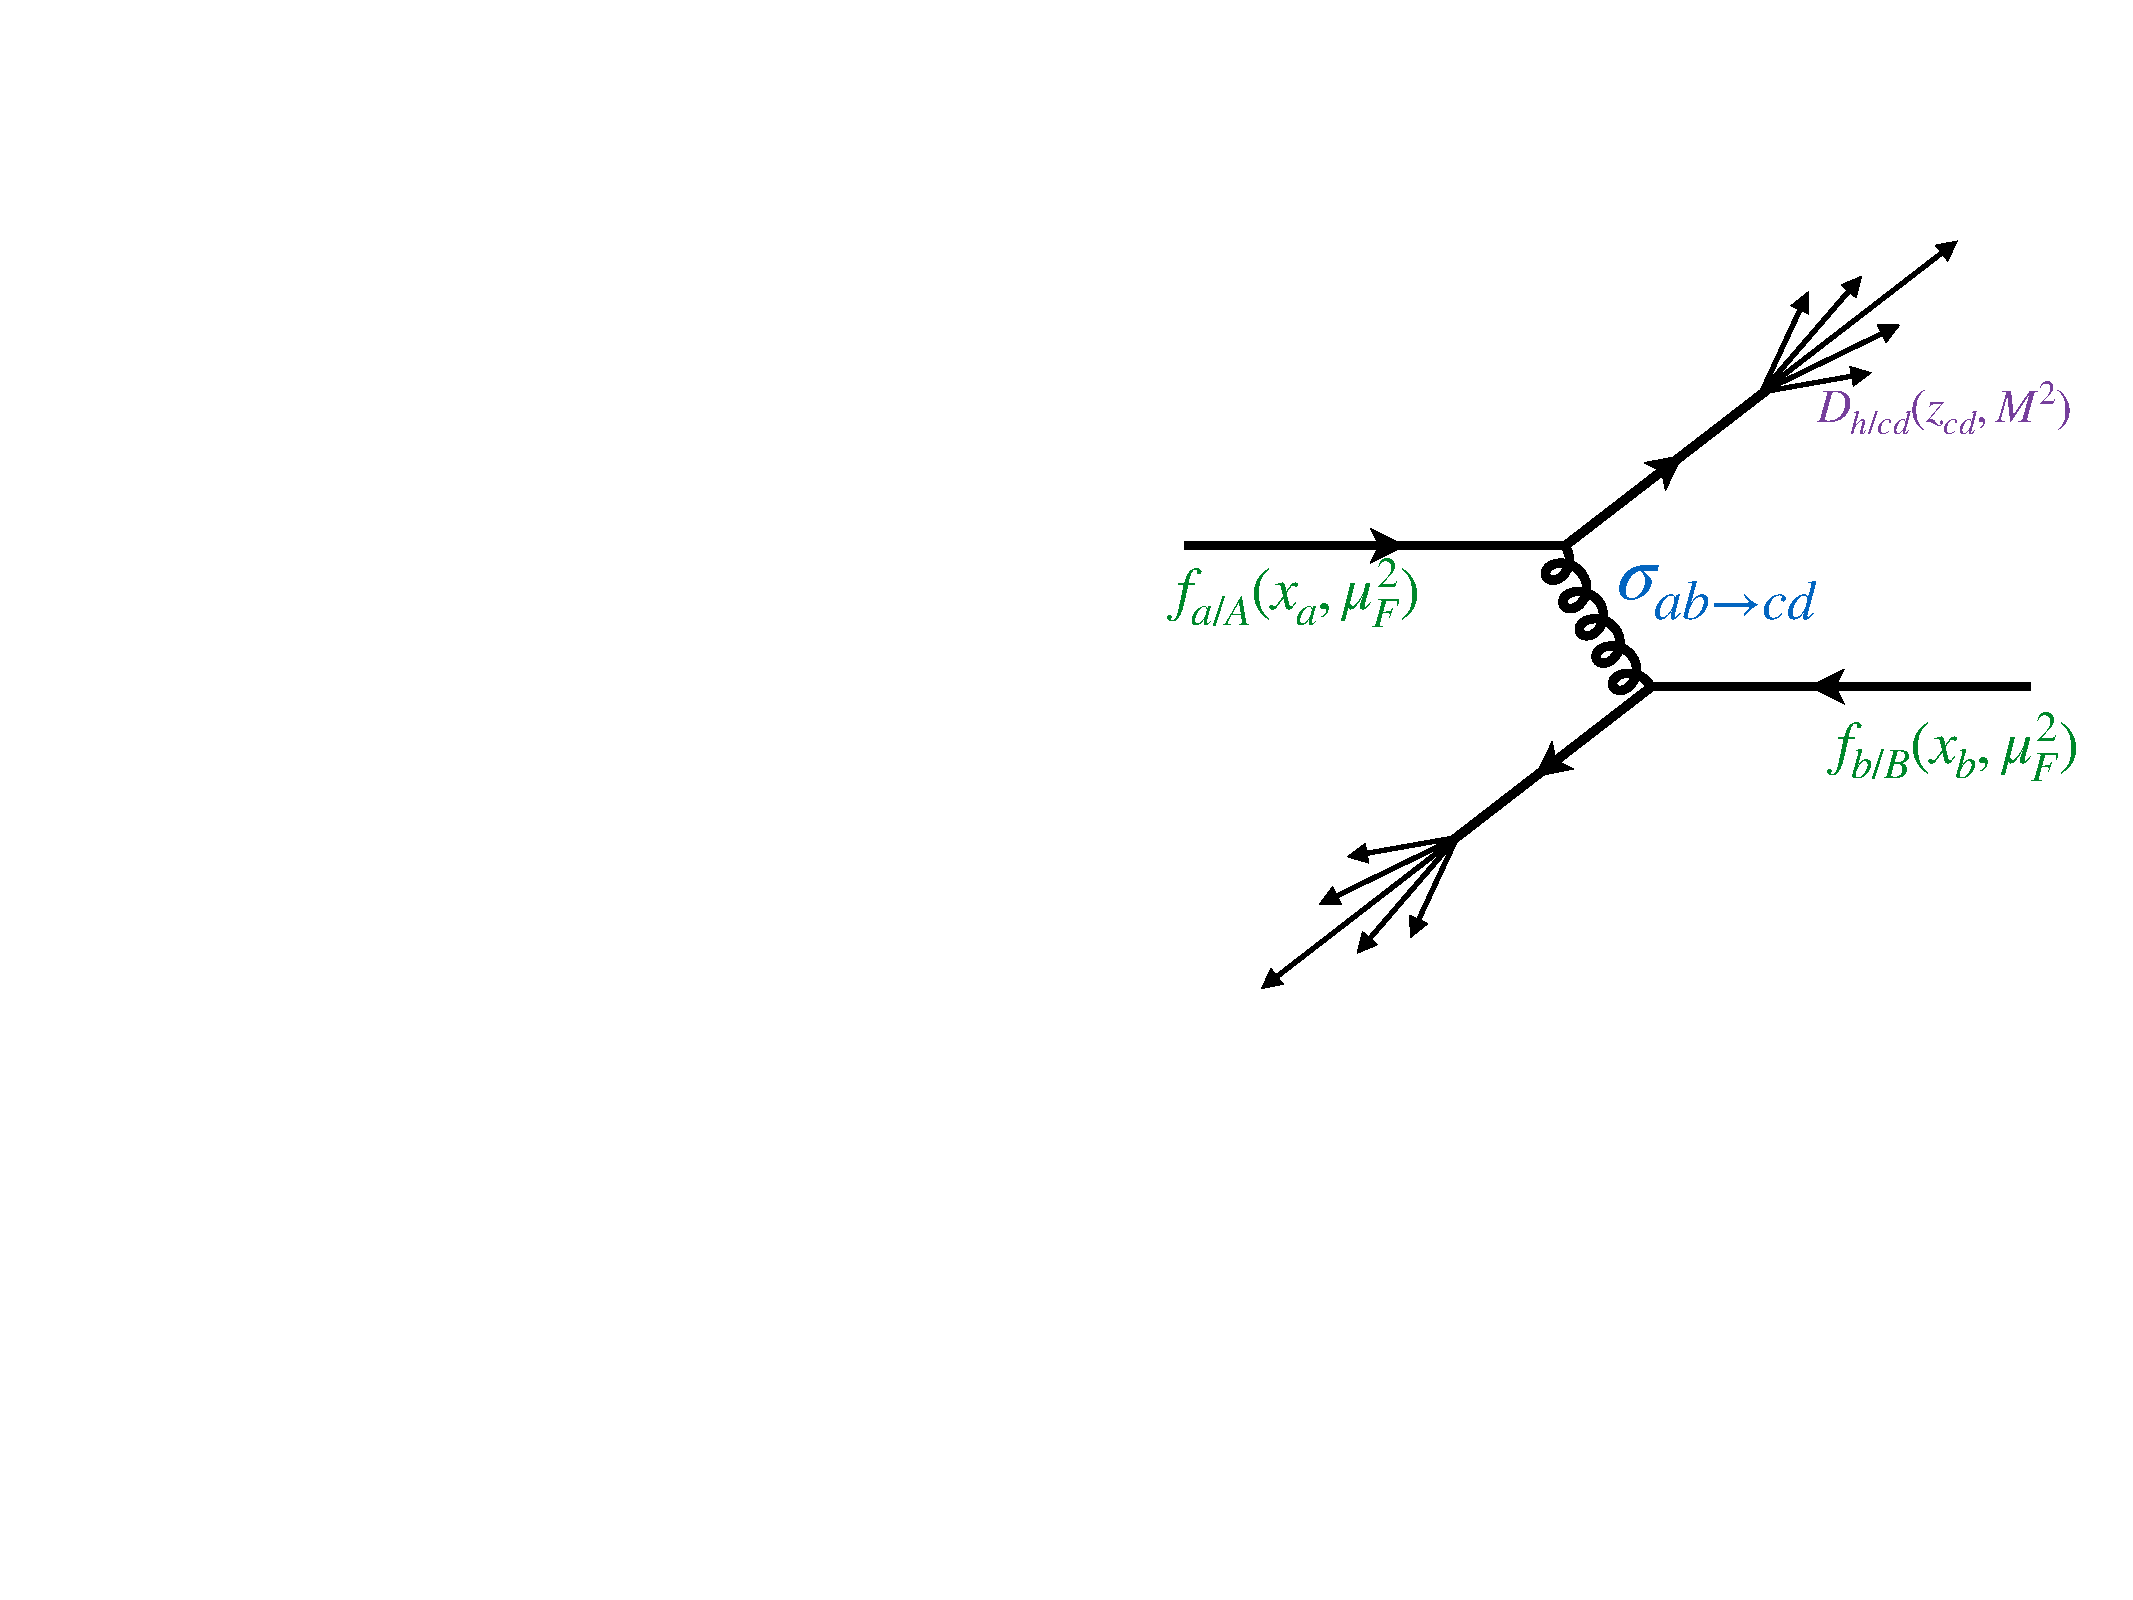
\includegraphics[width=0.35\textwidth]{figures/theory/feynman_jet}
\caption{Jet production from the process $pp \rightarrow hX$, factorizing in terms of the parton distribution functions, scattering cross sections, and jet fragmentation functions. \cite{Qin:2015srf}}
\label{fig:feynman_jet}
\end{center}
\end{figure}



\begin{align}
\label{eq:hadronCS}
d \sigma_{pp \rightarrow hX} \approx & \sum_{abjd} \int dx_a \int dx_b \int dz_j f_{a/p} (x_a, \mu_f) \otimes f_{b/p} (x_b, \mu_f) \\
& \otimes d\sigma_{ab\rightarrow jd} (\mu_f, \mu_F, \mu_R)  \nonumber \\
& \otimes D_{j \rightarrow h} (z_j, \mu_f) \nonumber
\end{align}
where $x_a = p_a/P_A, x_b = p_b / P_b$ are the initial momentum fractions carried by the interacting partons, $z_j = p_h / p_j$ is the momentum fraction carried by the final observed hadron. $f_{a/p} (x_a, \mu_f)$ and $f_{b/p} (x_b, \mu_f)$ are the two parton distribution functions (PDFs), $d\sigma_{ab\rightarrow jd} (\mu_f, \mu_F, \mu_R)$ is the differential cross section for parton scattering and $D_{j\rightarrow }(z_j,\mu_F)$ is the fragmentation function (FFs) for parton $j$ to hadron $h$. $\mu_f$ and $\mu_F$ are the factorization scales and $\mu_R$ is the renormalization scale, and are typically taken to be the same hard scale $Q$. The PDFs characterize the initial state and represent the probability of finding a parton with momentum fraction $x$ (shown in Figure~\ref{fig:bjorkenX}) in the initial hadron, while the FFs describe the probability of fragmenting to a hadron $h$ with given kinematic properties.

\begin{figure}[htbp]
\begin{center}
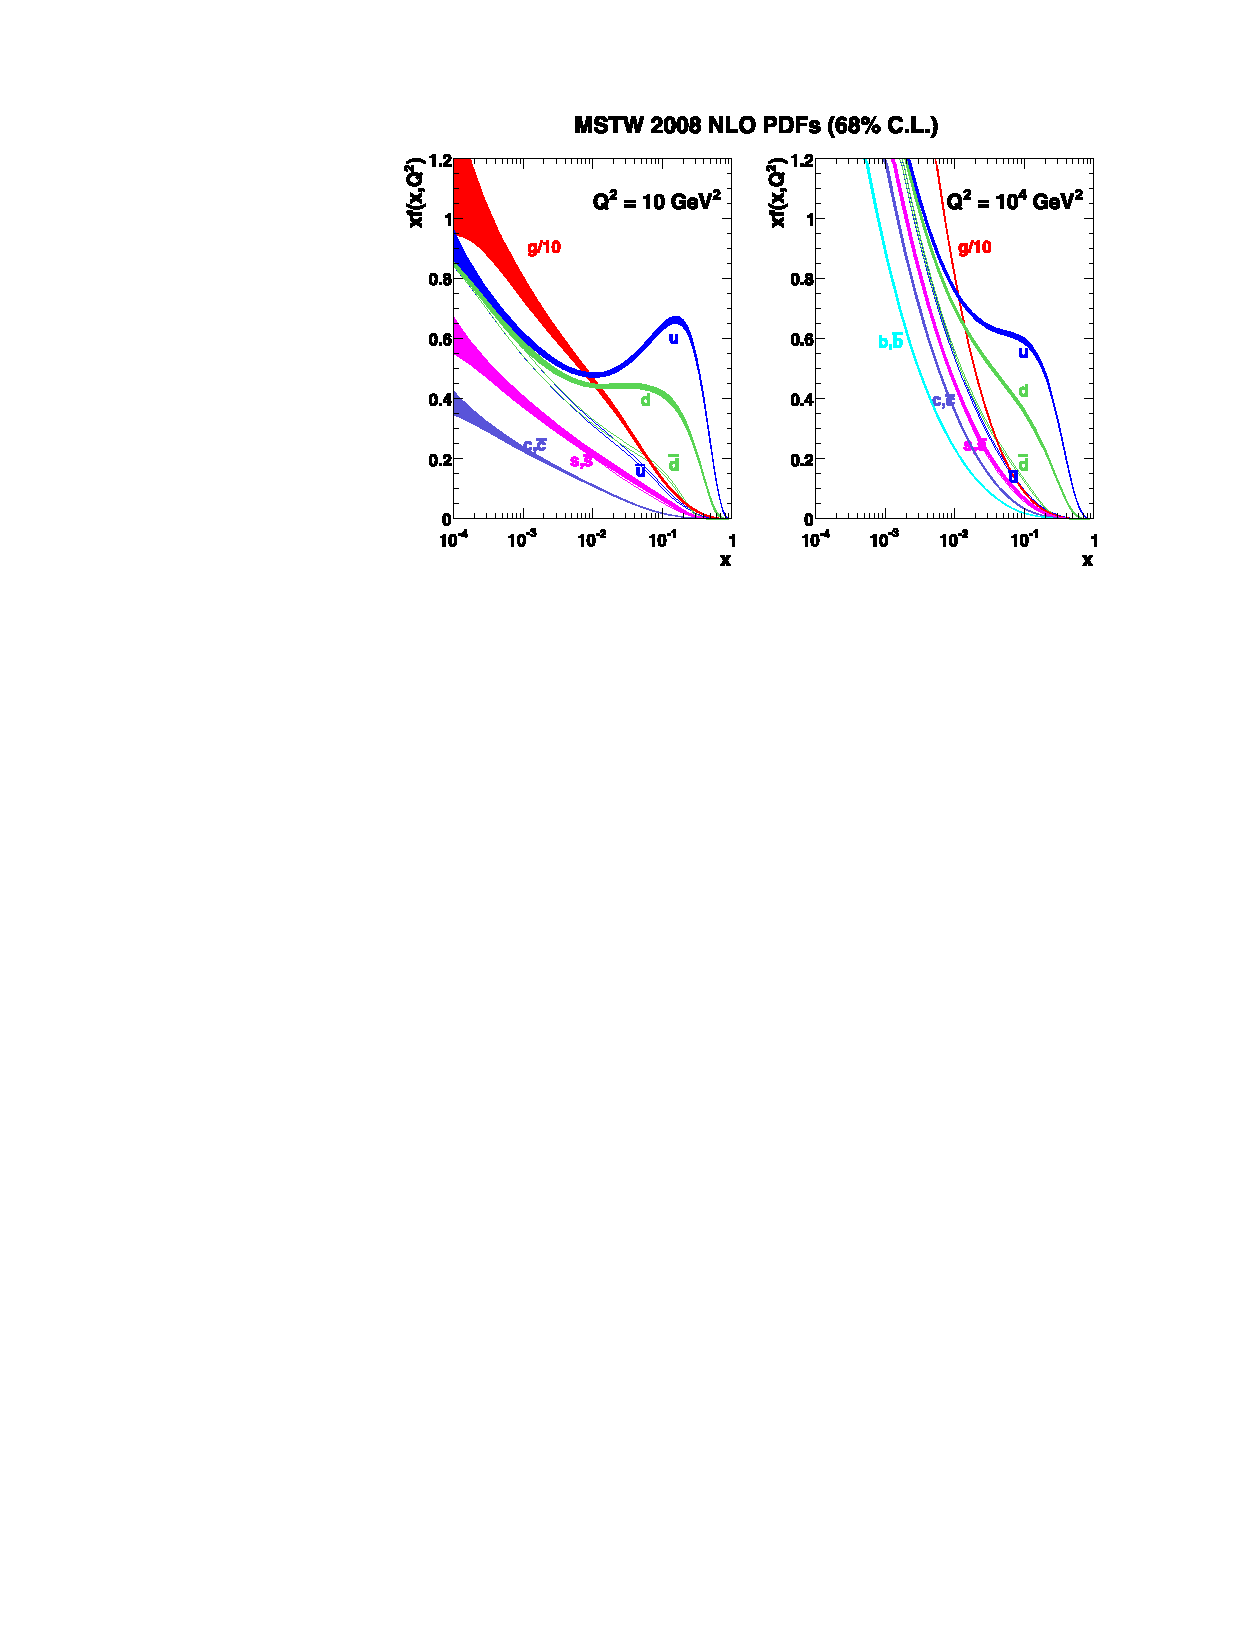
\includegraphics[width=0.55\textwidth]{figures/theory/bjorkenX}
\caption{The next to leading order (NLO) PDFs at (left) $Q^2 = 10 \mathrm{GeV}^2$ and (right) $Q^2 = 10^4 \mathrm{GeV}^2$. The band is the associated one-sigma (68\%) confidence level uncertainty. Taken from \cite{Martin2009}}
\label{fig:bjorkenX}
\end{center}
\end{figure}


%Both the PDFs and FFs are universal and their scale dependence evolves via the Dokshitzer-Gribov-Lipatov-Altarelli-Parisi (DGLAP) equations \cite{ALTARELLI1977298, Gribov:1972ri, Dokshitzer:1977sg}. These calculations can be compared to the inclusive charged particle distributions in \sqrts = 13 TeV \pp\ collisions and shown in Figure~\ref{fig:inclhadronCS}.  



%The energy lost by a jet serves as further confirmation that the medium produced in a heavy ion collision is strongly coupled.

In the case of heavy ion collisions, the jet observables can be modified due to two sources: the nuclear PDF being distinct from a proton PDF, and the formation of the quark gluon plasma.

The former is collectively referred to as cold nuclear matter (CNM) effect, and can be quantified by defining a nuclear modification factor for the PDF:

\begin{align}
R_a^A (x, Q^2) = \frac{f_{a/A} (x, Q^2)}{f_{a/p}(x, Q^2)}
\end{align}
where $f_{a/A}$ and $f_{a/p}$ are the nuclear and proton PDFs respectively. This $R_a^A$ factor is determined by global fits to data from DIS measurements \cite{PhysRevC.76.065207, PhysRevD.69.074028, Eskola_2009}. CNM effects include the following contributions:
\begin{itemize}
\item Shadowing: This is a destructive interference effect that reduces the interactions of a nucleon incident on a nucleus within its interior and on its back face. This effect reduces the effective number of nucleons in an inelastic interaction to $A^{2/3}$. For $Q^2$ of the order of a few $\mathrm{GeV}^2$, this effect dominates for $x < 0.05$ and implies $R_a^A (x, Q^2) < 1$  \cite{PhysRevLett.64.1342}.
\item Anti-shadowing: This compensates for the shadowing effect based on the momentum sum rule, and for $Q^2$ of the order of a few $\mathrm{GeV}^2$ implies $R_a^A (x, Q^2) > 1$ over the region $0.05 < x < 0.20$.
\item EMC: The modification of the nuclear structure function was first observed by the European Muon Collaboration \cite{AUBERT1983275}. Recent observations have suggested that the effect is caused by short-range correlated nucleon pairs within nuclei \cite{PhysRevC.85.047301}. For $Q^2$ of the order of a few $\mathrm{GeV}^2$, this effect dominates for $0.2 < x < 0.80$ and implies $R_a^A (x, Q^2) < 1$.
\item  Fermi Motion: This effect considers the motion of the nucleons within the nucleus. It results in $R_a^A (x, Q^2) > 1$  over the $x > 0.8$ region for $Q^2$ of the order of a few $\mathrm{GeV}^2$ \cite{Saito:1985ct}.
\end{itemize}

Cold nuclear matter effects are experimentally measured using $p+A$ systems where the size and shape of the plasma, and hence any effects thereof, are a lot smaller. 

The second source of modification is the formation of the hot and dense quark gluon plasma. The hot nuclear matter effects further serve as an independent confirmation that the medium formed is strongly interacting. Jets are formed early enough that they traverse the Quark Gluon Plasma and as strongly interacting particles, are both affected by, and affect the QGP. This interaction typically results in the jet losing energy and forward momentum \cite{2012176, ATLAS:2017wvp}, with the lost energy being deposited in the medium \cite{Khachatryan2016}. Jets can also pick up momentum transverse to the parton direction \cite{Chatrchyan:2012nia}. The hot nuclear matter effects can be considered to be a combination of collisional and radiative energy losses summarized in Figure~\ref{fig:jetEnergyLoss}.

\begin{figure}[htbp]
\begin{center}
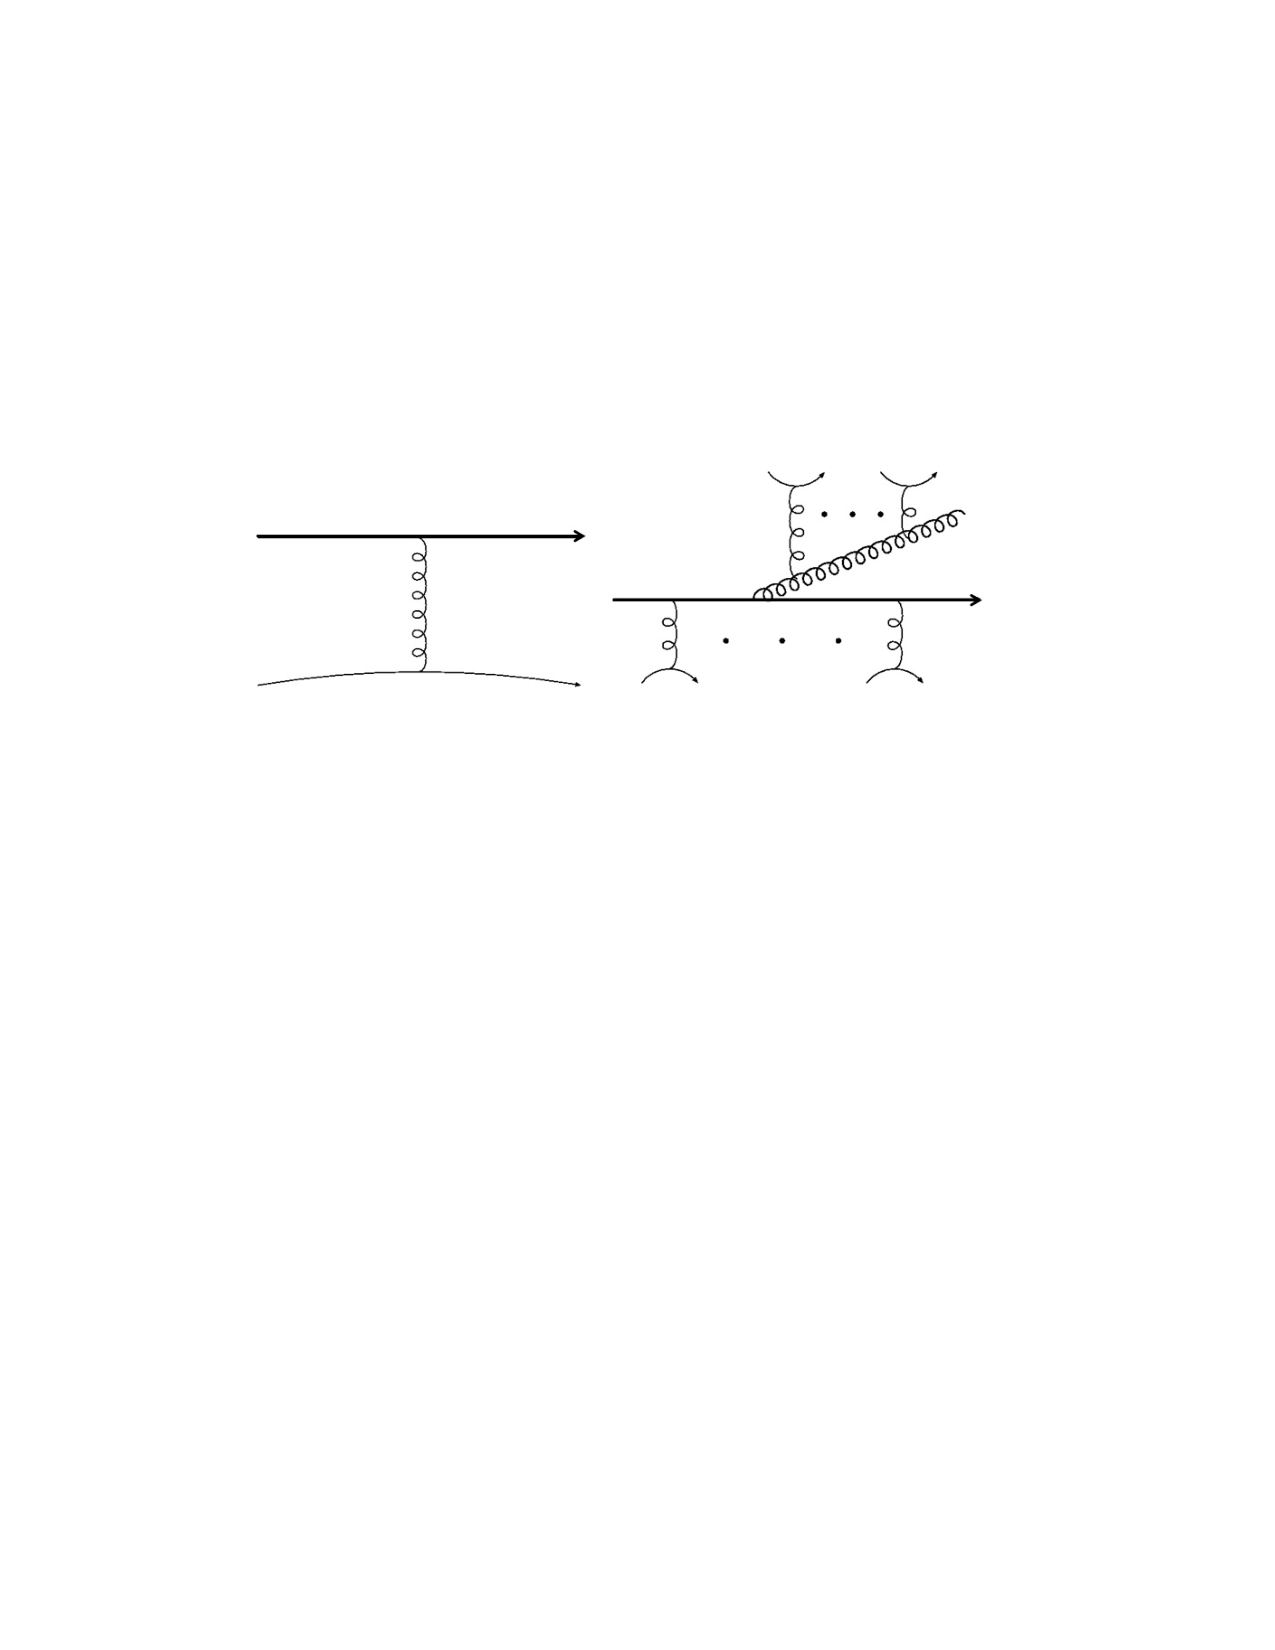
\includegraphics[width=0.75\textwidth]{figures/theory/jetEnergyLoss}
\caption{The typical diagrams for (left) collisional and (right) radiative energy losses for a parton in a hard scattering as it propagates through the QGP. Taken from \cite{Qin:2015srf}}
\label{fig:jetEnergyLoss}
\end{center}
\end{figure}

\begin{itemize}
\item Collisional energy loss: This is a combination of elastic and inelastic collisions of the hard parton with the constituents of the quark gluon plasma. 
\item Radiative energy loss: This is the larger source of parton energy loss and jet quenching. These are modified by the presence of the plasma due to scatterings off of the plasma constituents. A variety of radiative energy loss frameworks that have been developed include: Baier-Dokshitzer-Mueller-Peigne-Schiff-Zakharov (BDMPS-Z) \cite{BAIER1997291}, Gyulassy, Levai and Vitev (GLV) \cite{Gyulassy:1999zd}, Amesto-Salgado-Wiedemann (ASW) \cite{Wiedemann:2000za},  Arnold-Moore-Yaffe (AMY) \cite{Arnold:2001ba} and higher twist (HT) \cite{Guo:2000nz}.
\end{itemize}

\subparagraph{Collisional energy loss} This is a combination of elastic and inelastic collisions of the hard parton with the constituents of the quark gluon plasma. The 

Both hot and cold nuclear matter effects can be described by modifying Equation~\ref{eq:hadronCS} as:
\begin{align}
d \sigma_{AB \rightarrow hX}  \approx & \sum_{abjj'd} f_{a/A} (x_a) \otimes f_{b/B} (x_b) \\ 
& \otimes d\sigma_{ab\rightarrow jd} (\mu_f, \mu_F, \mu_R)  \nonumber \\
& \otimes P_{j\rightarrow j'} \nonumber \\
& \otimes D_{h \rightarrow j'} (z_j, \mu_f) \nonumber 
\end{align}

where the additional $P_{j\rightarrow j'}$ describes the interaction of the hard parton with the colored medium. This is typically taken as part of the fragmentation modification as:

\begin{align}
\widetilde{D}_{h \rightarrow j'} (z_j, \mu_f) \approx \sum_{j'} P_{j\rightarrow j'} (p_{j'} | p_j) \otimes D_{h\rightarrow j'} (_{j'})
\end{align}


\subsection{Jet Reconstruction}
Jets can reconstructed by clustering algorithms that take in a variety of inputs. The algorithm used in ATLAS is the \antikt\ clustering algorithm \cite{Cacciari:2008gp}. This algorithm clusters soft particles around hard ones in the following manner:

\begin{itemize}
\item Calculate all distances $d_{ij}$ between entities $i$ and $j$, and distance $d_{iB}$ between entity $i$ and beam $B$.
\item Identify the smallest distances such that for the smallest distance $d_{ij}$, the entities $i$ and $j$ are combined and return to beginning.
\item If the smallest distance is $d_{iB}$, then take $i$ as the jet and remove it from the list of entities and return to beginning.
\item Continue the procedure till the list of items is empty.
\end{itemize}

In general the distance $d_{ij}$ between the objects is found the via the prescription

\begin{align}
d_{ij} &= \mathrm{min} (k_{Ti}^{2p} , k_{Tj}^{2p}) \frac{\Delta_{ij}^2}{R^2}  \\
d_{iB} &= k_{Ti}^{2p}
\end{align}

where $k_{Ti}$ is the transverse momentum of particle $i$ and $\Delta_{ij} = \sqrt{\Delta\eta_{ij}^2 + \Delta\phi_{ij}^2}$ is the distance between particles $i$ and $j$ in $\eta-\phi$ space. $R$ the distance parameter and reflects the size of the jet being considered. In the case of the \antikt\ algorithm, $p = -1$. Other popular clustering algorithms like \kt\ \cite{Catani:1993hr} and Cambridge/Aachen \cite{Dokshitzer:1997in} use $p = 1$ and $p=0$ respectively. The behavior of the different clustering algorithms is shown in Figure~\ref{fig:JetClustering}. 

\begin{figure}[htp]
\centering
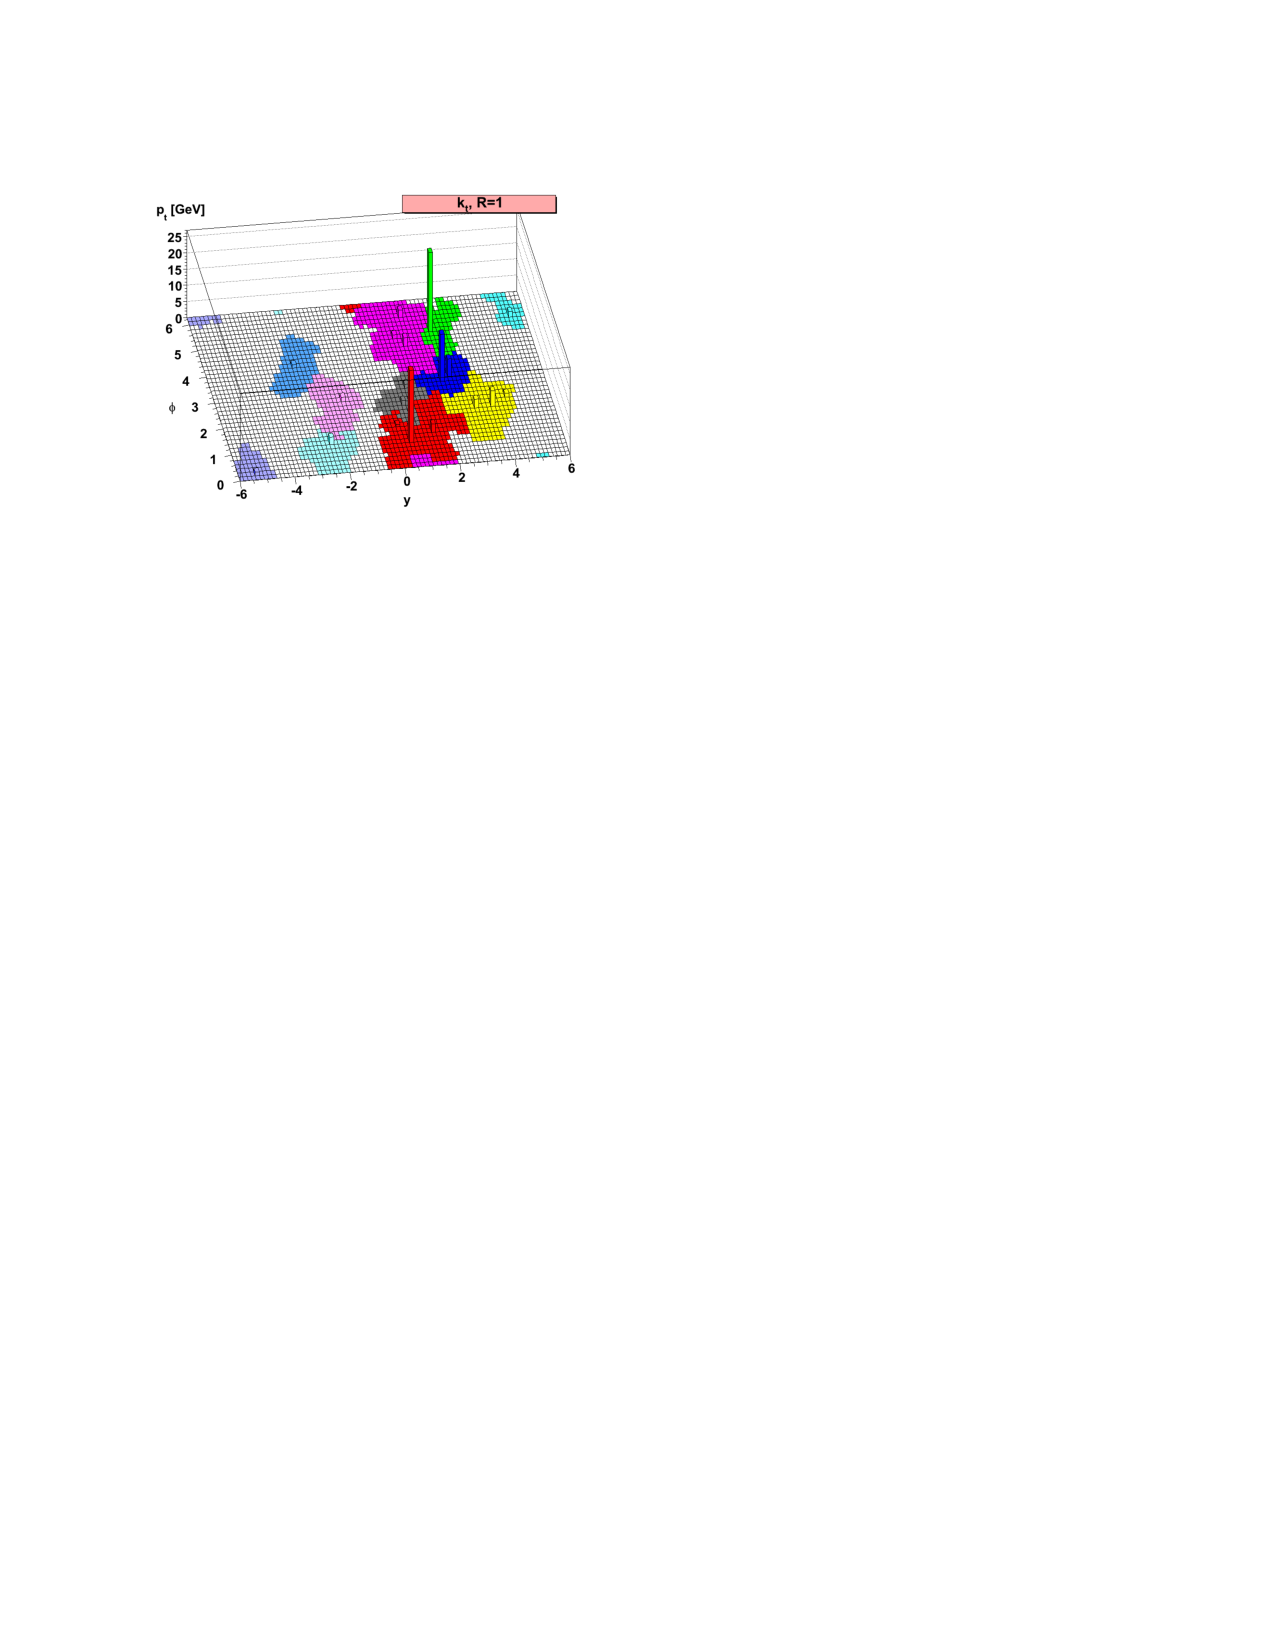
\includegraphics[width=.3\textwidth]{jetMeasurements/jetReco_kt}\hfill
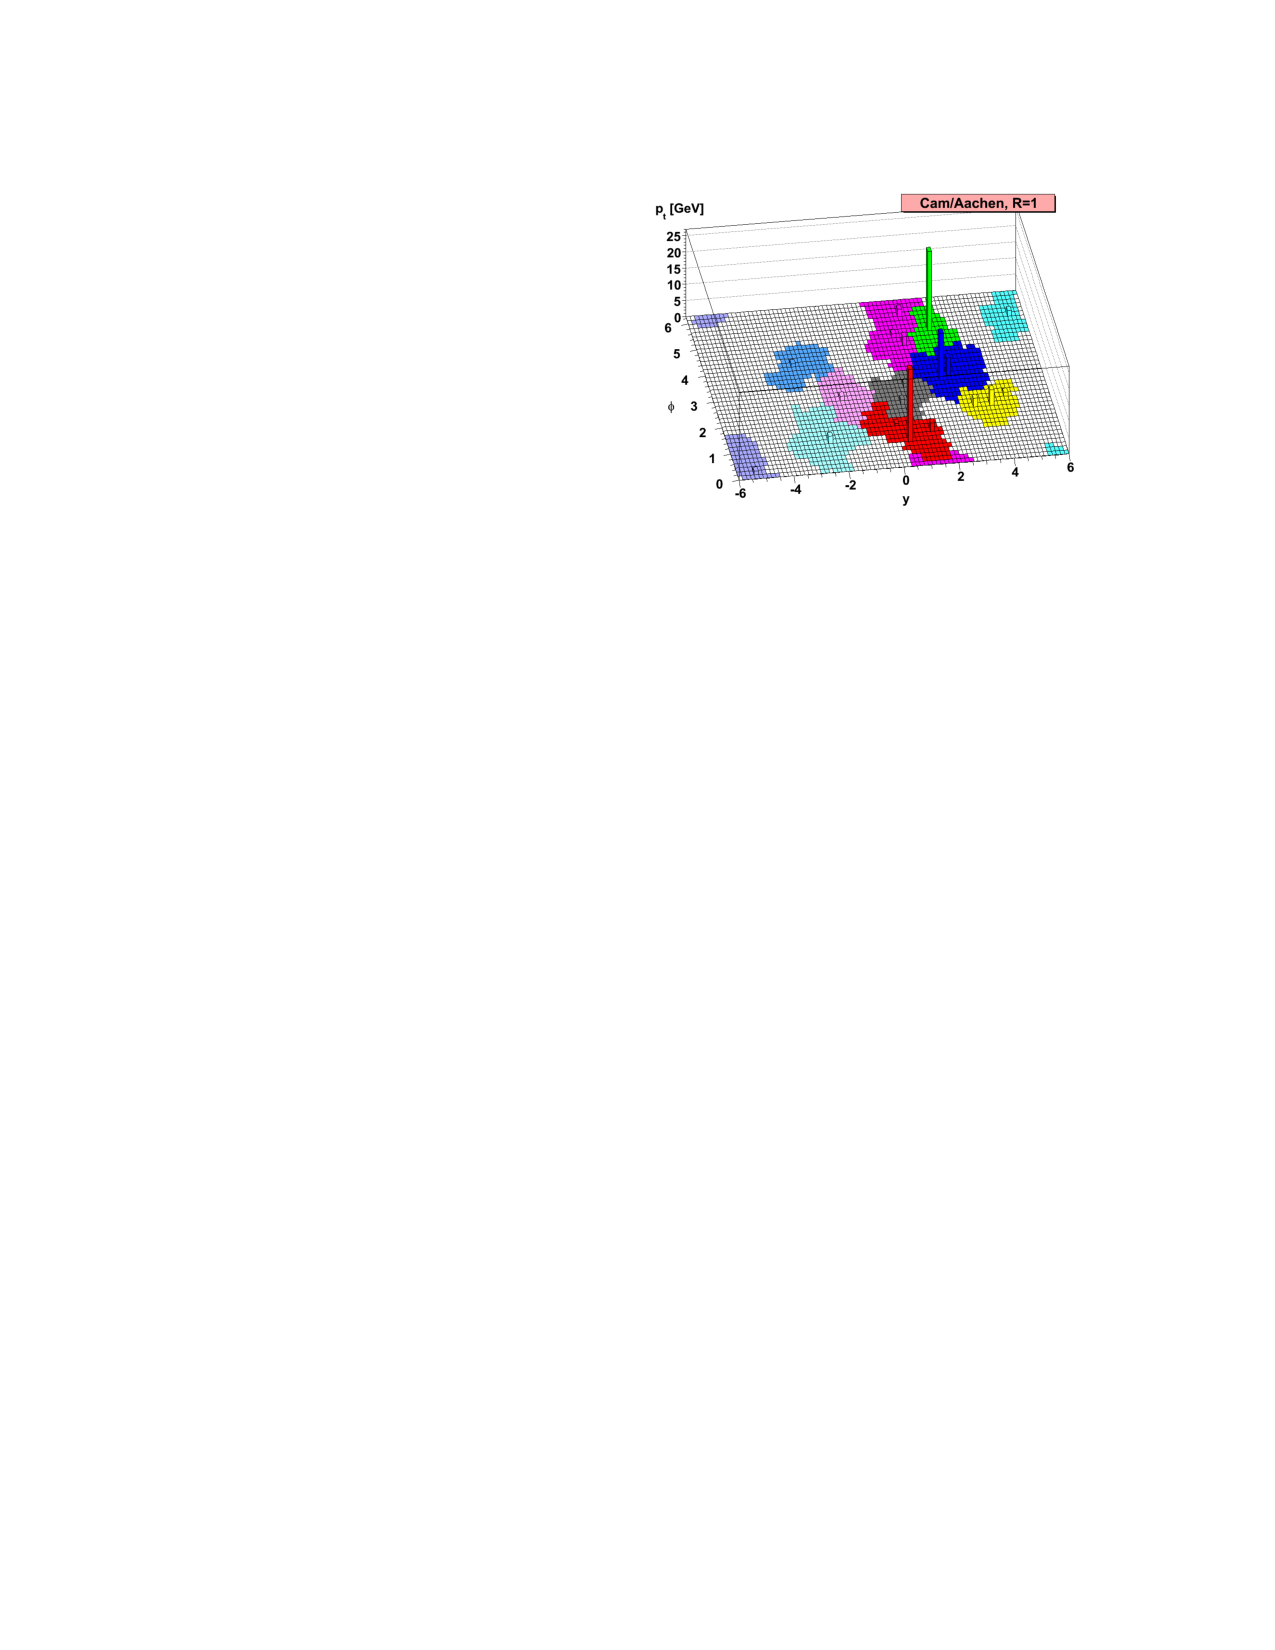
\includegraphics[width=.3\textwidth]{jetMeasurements/jetReco_CA}\hfill
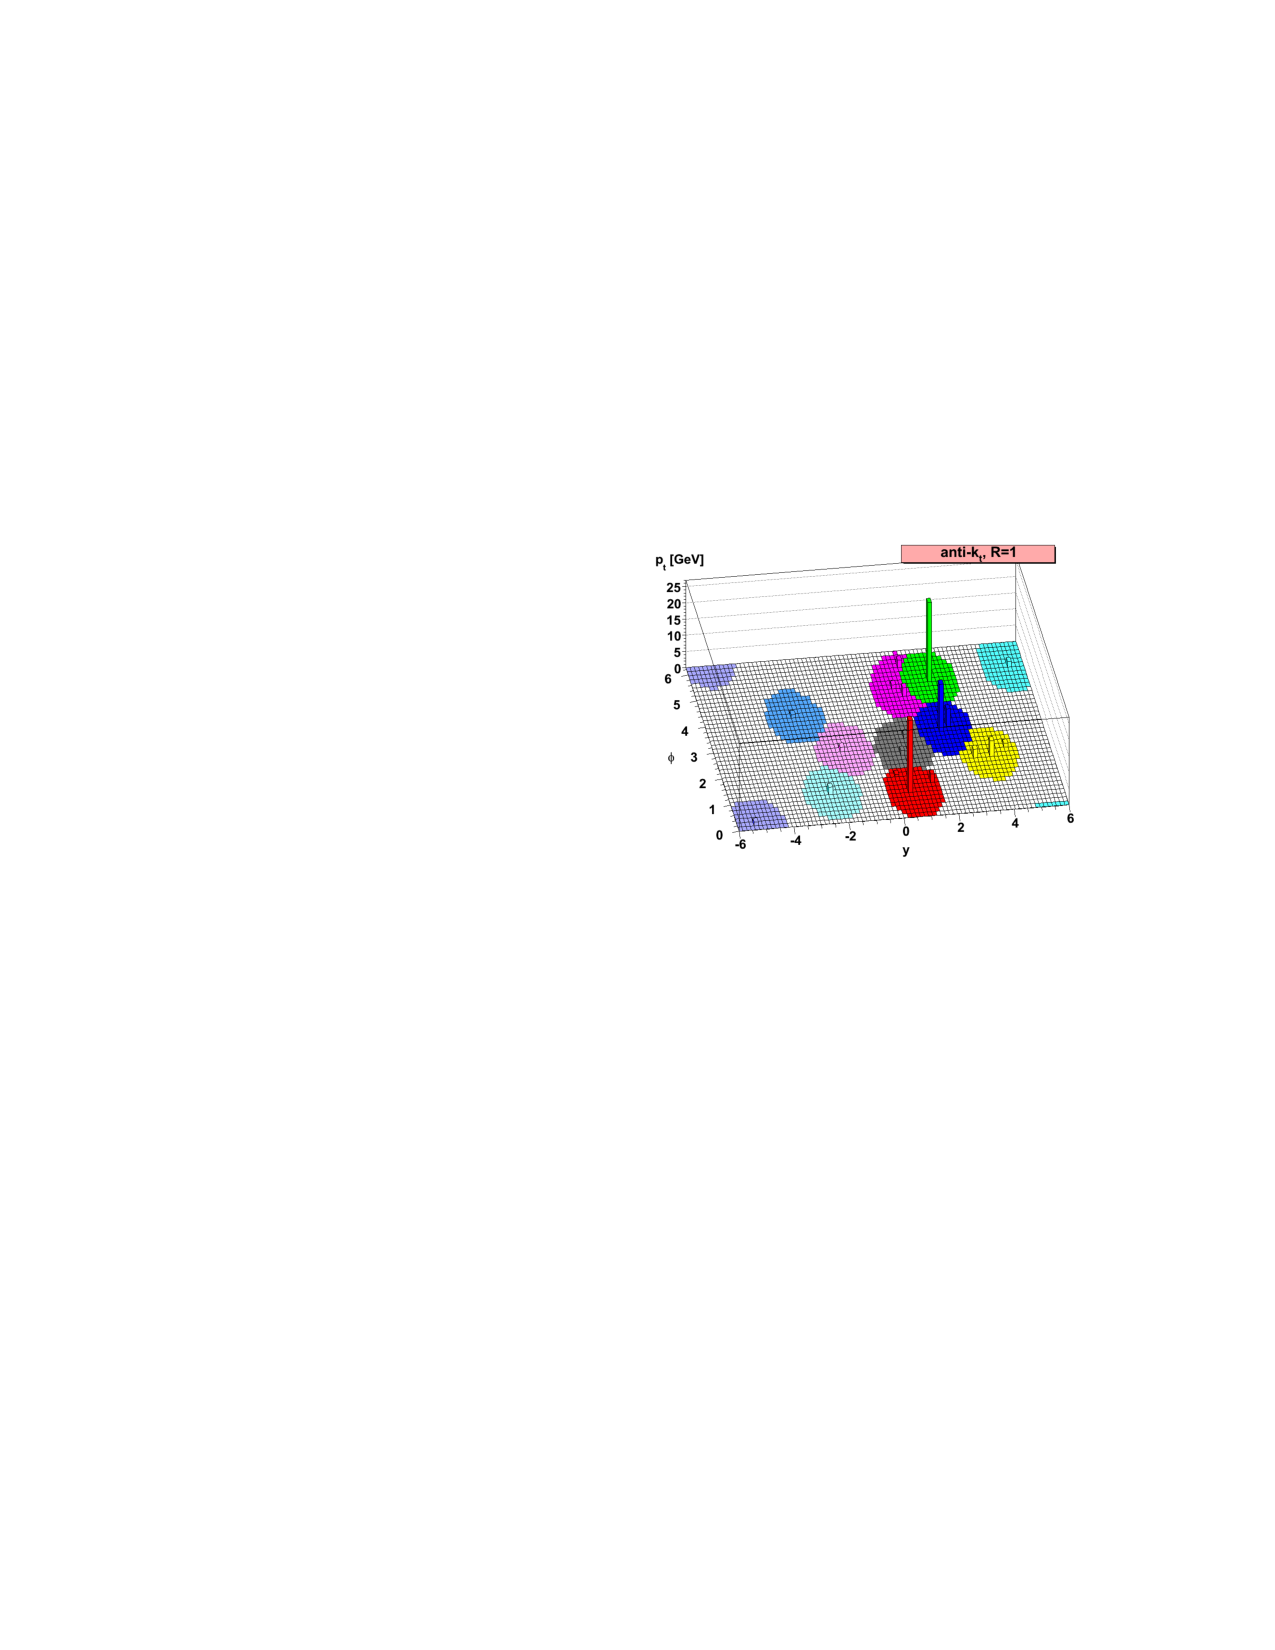
\includegraphics[width=.3\textwidth]{jetMeasurements/jetReco_antikt}\hfill
\caption{Different clustering algorithms applied to the sample parton-level event. Figure taken from \cite{Cacciari:2008gp}.}
\label{fig:JetClustering}
\end{figure}

The popularity of the \antikt\ algorithm comes from its overcoming of two common problems: collinear and infrared safety. These are related to instabilities in the cones that are found due to soft radiation. 

Figure~\ref{fig:collinearSafe} describes the collinear safety problem. In a collinear safe jet algorithm, the presence of a virtual loop or a collinear splitting of a central particle would not change the number of jets being reconstructed. On the other hand, while a collinear unsafe jet algorithm would not change its output with the presence of a virtual loop, a splitting in the central particle would lead to the left and right most particles forming individual seeds, implying two reconstructed jets \cite{Salam:2009jx}.

\begin{figure}[htp]
\centering
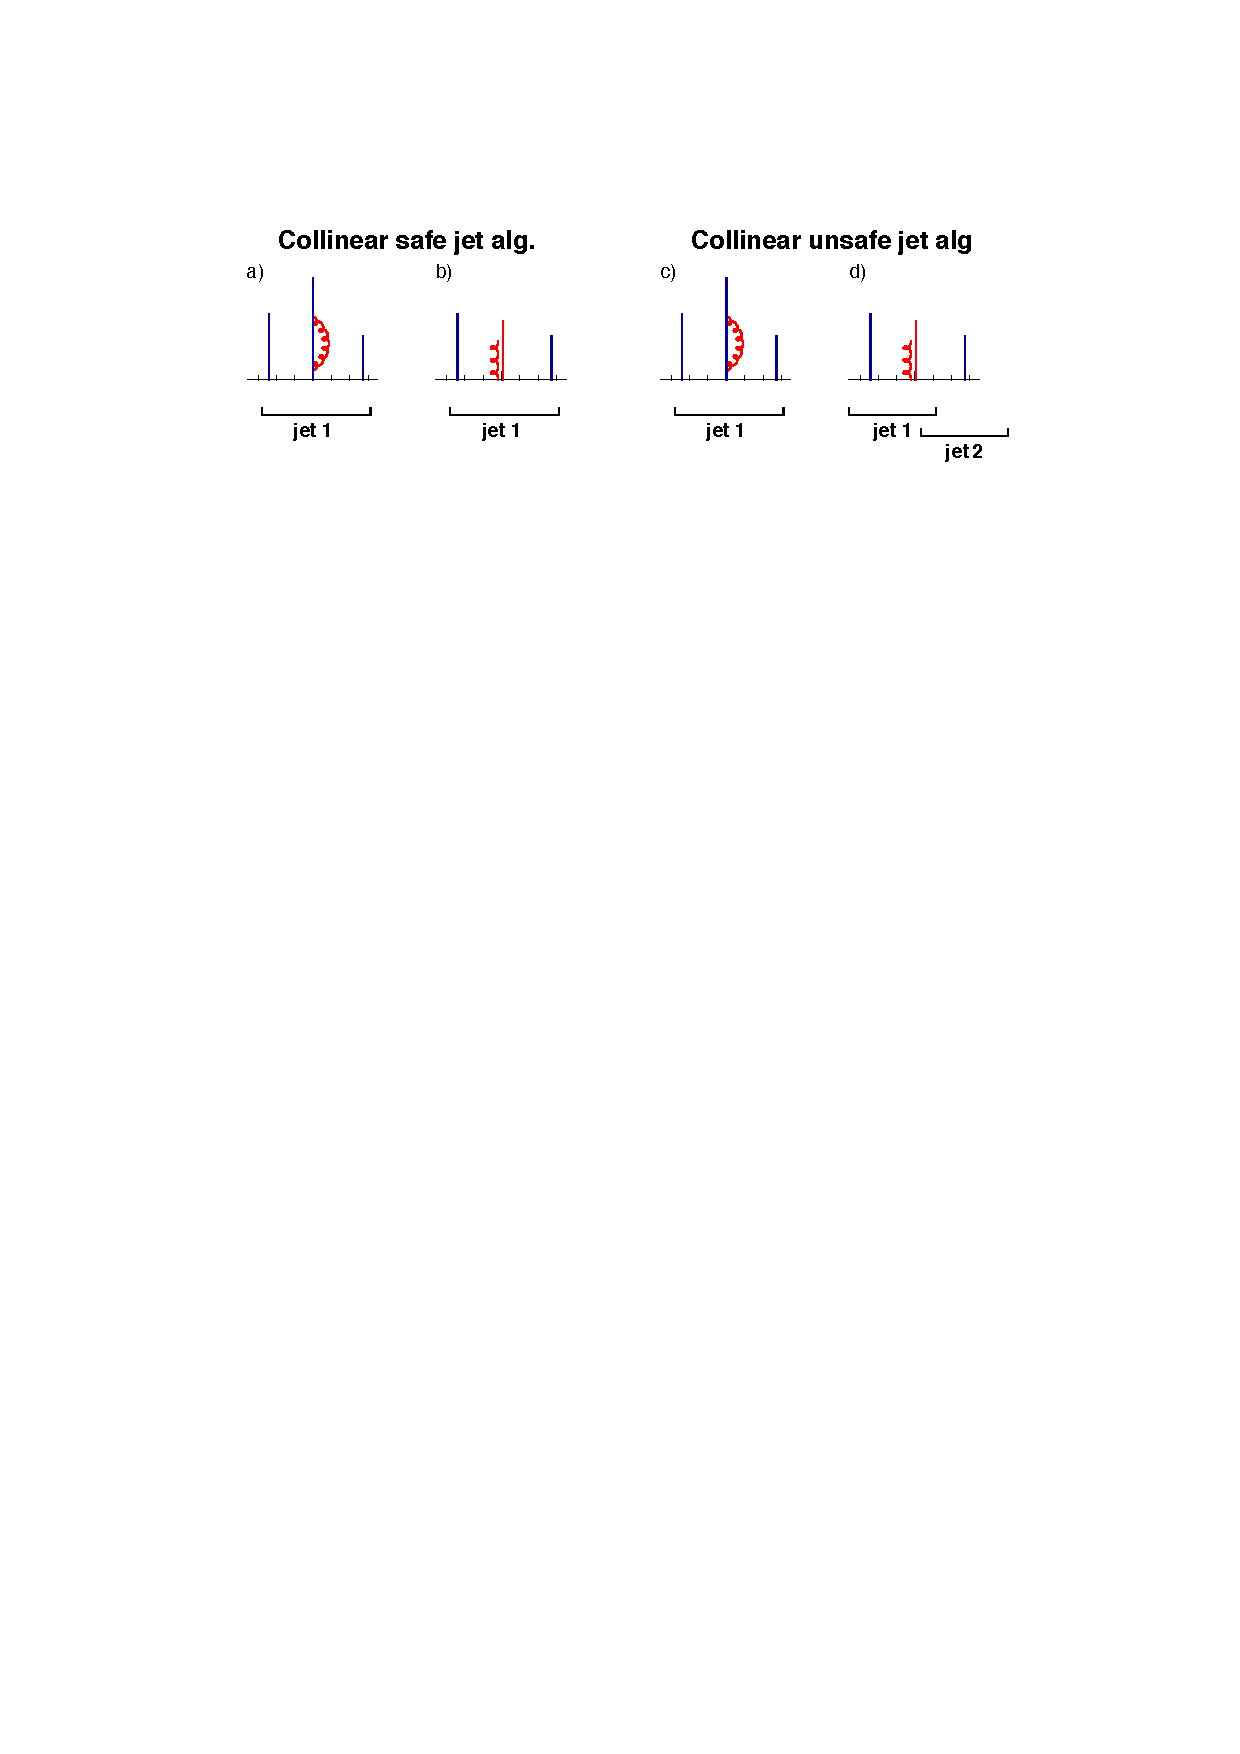
\includegraphics[width=.75\textwidth]{jetMeasurements/collinearSafe}
\caption{An illustration of collinear unsafe behavior. The particle \pt\ is proportional to the height and the horizontal axis indicates rapidity. Taken from \cite{Salam:2009jx}. }
\label{fig:collinearSafe}
\end{figure}


A schematic describing infrared un-safety is shown in Figure~\ref{fig:infraredSafe}. Here an infrared safe algorithm would use the three particles as seeds iteratively find two stable cones. An unsafe algorithm however would find three overlapping cones based on the addition of a soft seed.

\begin{figure}[htp]
\centering
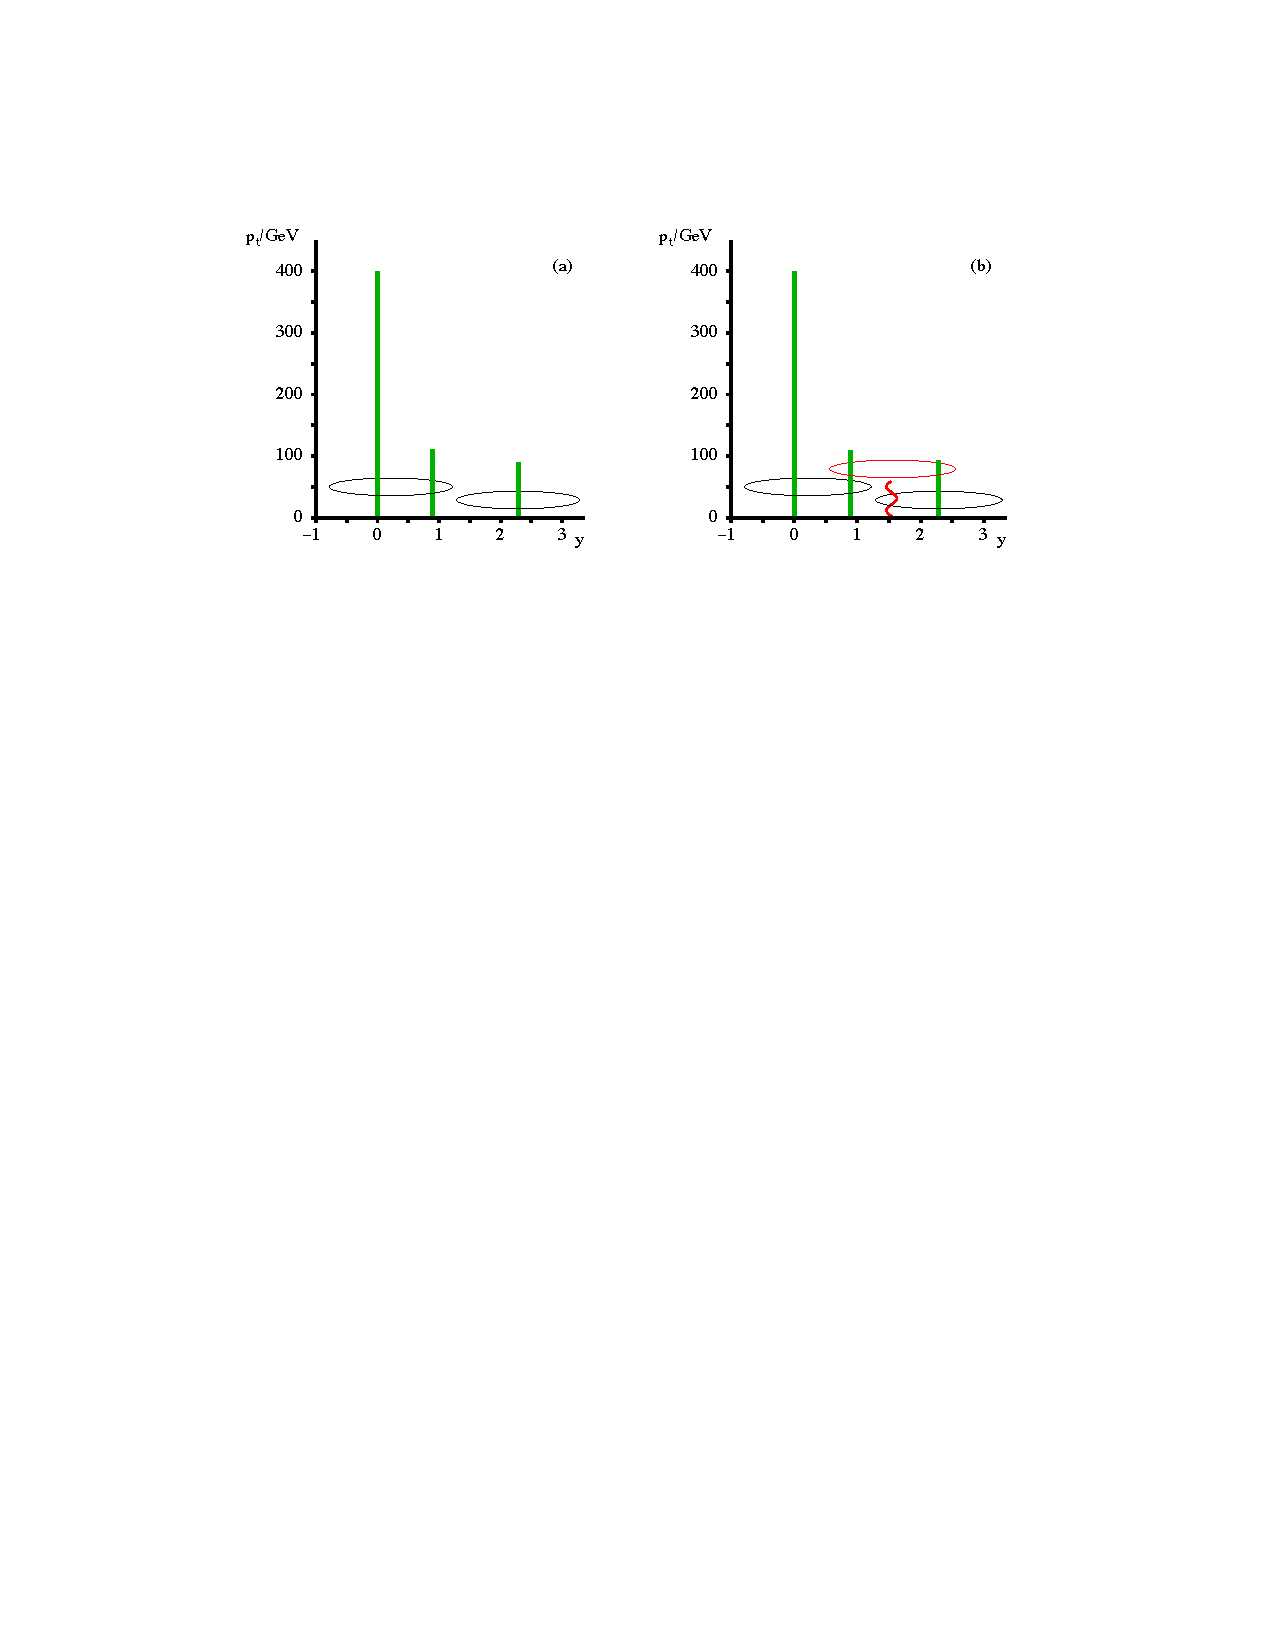
\includegraphics[width=.65\textwidth]{jetMeasurements/infraredSafe}
\caption{An illustration of infrared unsafe behavior. The particle \pt\ is proportional to the height and the horizontal axis indicates rapidity. Taken from \cite{Salam_2007} }
\label{fig:infraredSafe}
\end{figure}

% the \antikt\ reconstruction algorithm is used with the distance parameter $R=0.4$

For heavy ion collisions in ATLAS, the inputs to the algorithm are the $\eta \times \phi = 0.1 \times 0.1$ calorimeter towers. The tower energies are determined by summing up the energies of the individual calorimeter cells. The \antikt\ algorithm is first run with the distance parameter $R=0.2$, following which an underlying event subtraction procedure is performed. A first estimate of the average underlying event energy density $\rho_i (\eta)$ is done in 0.1 slices of $\eta$ in each calorimeter layer $i$ after excluding the regions that overlap with the seed jets. A modulation of $2v_{2} \cos[2(\phi-\Psi_2)] $ is applied to account for the flow from the QGP and the underlying event is subtracted to give $E_{Tj}^{\mathrm{sub}}$:

\begin{align}
E_{Tj}^{\mathrm{sub}} = E_{Tj} - A_j \rho_i (\eta_j) 1+2v_{2i} \big(\cos[2(\phi-\Psi_2)] \big)
\end{align}
where $ E_{Tj} , \eta_j, \phi_j$ and $A_j$ are the cell $E_T, \eta, \phi$ and area for cell $j$ in layer $i$. This process is done iteratively done one more time after getting new seeds with the distance parameter $R = 0.2$ and excluding areas that are within $\Delta R = 0.4$ of the seeds. Updated values of $\rho{'}_i$ and $v{'}_2$ are recalculated and used to estimate the background that is subtracted from the original cell energies. More details on this procedure can be found in \cite{2013220}.



%A few jet measurements and their modifications by the presence of the Quark Gluon Plasma are discussed in Section~\ref{sec:jetMeasurements}.
%

%%%%%%%%%%%%%%%%%%%%%%%%%%%%%%%%%%%%%%%%%%%%%%%%
%  jet cross section in  \sqrts = 13 TeV \pp\ collisions can be seen in Figure~\ref{fig:incljetCS}
%
%
%
%\begin{figure}[htbp]
%\begin{center}
%\includegraphics[width=0.55\textwidth]{figures/theory/incljetCS}
%\caption{The inclusive jet cross section as a function of \pt\ and $|y|$ as measured by ATLAS. The data are compared to NLO pQCD calculations. Taken from \cite{Aaboud:2017wsi}}
%\label{fig:incljetCS}
%\end{center}
%\end{figure}
%
%
%
%
%

%
%\begin{figure}[htbp]
%\begin{center}
%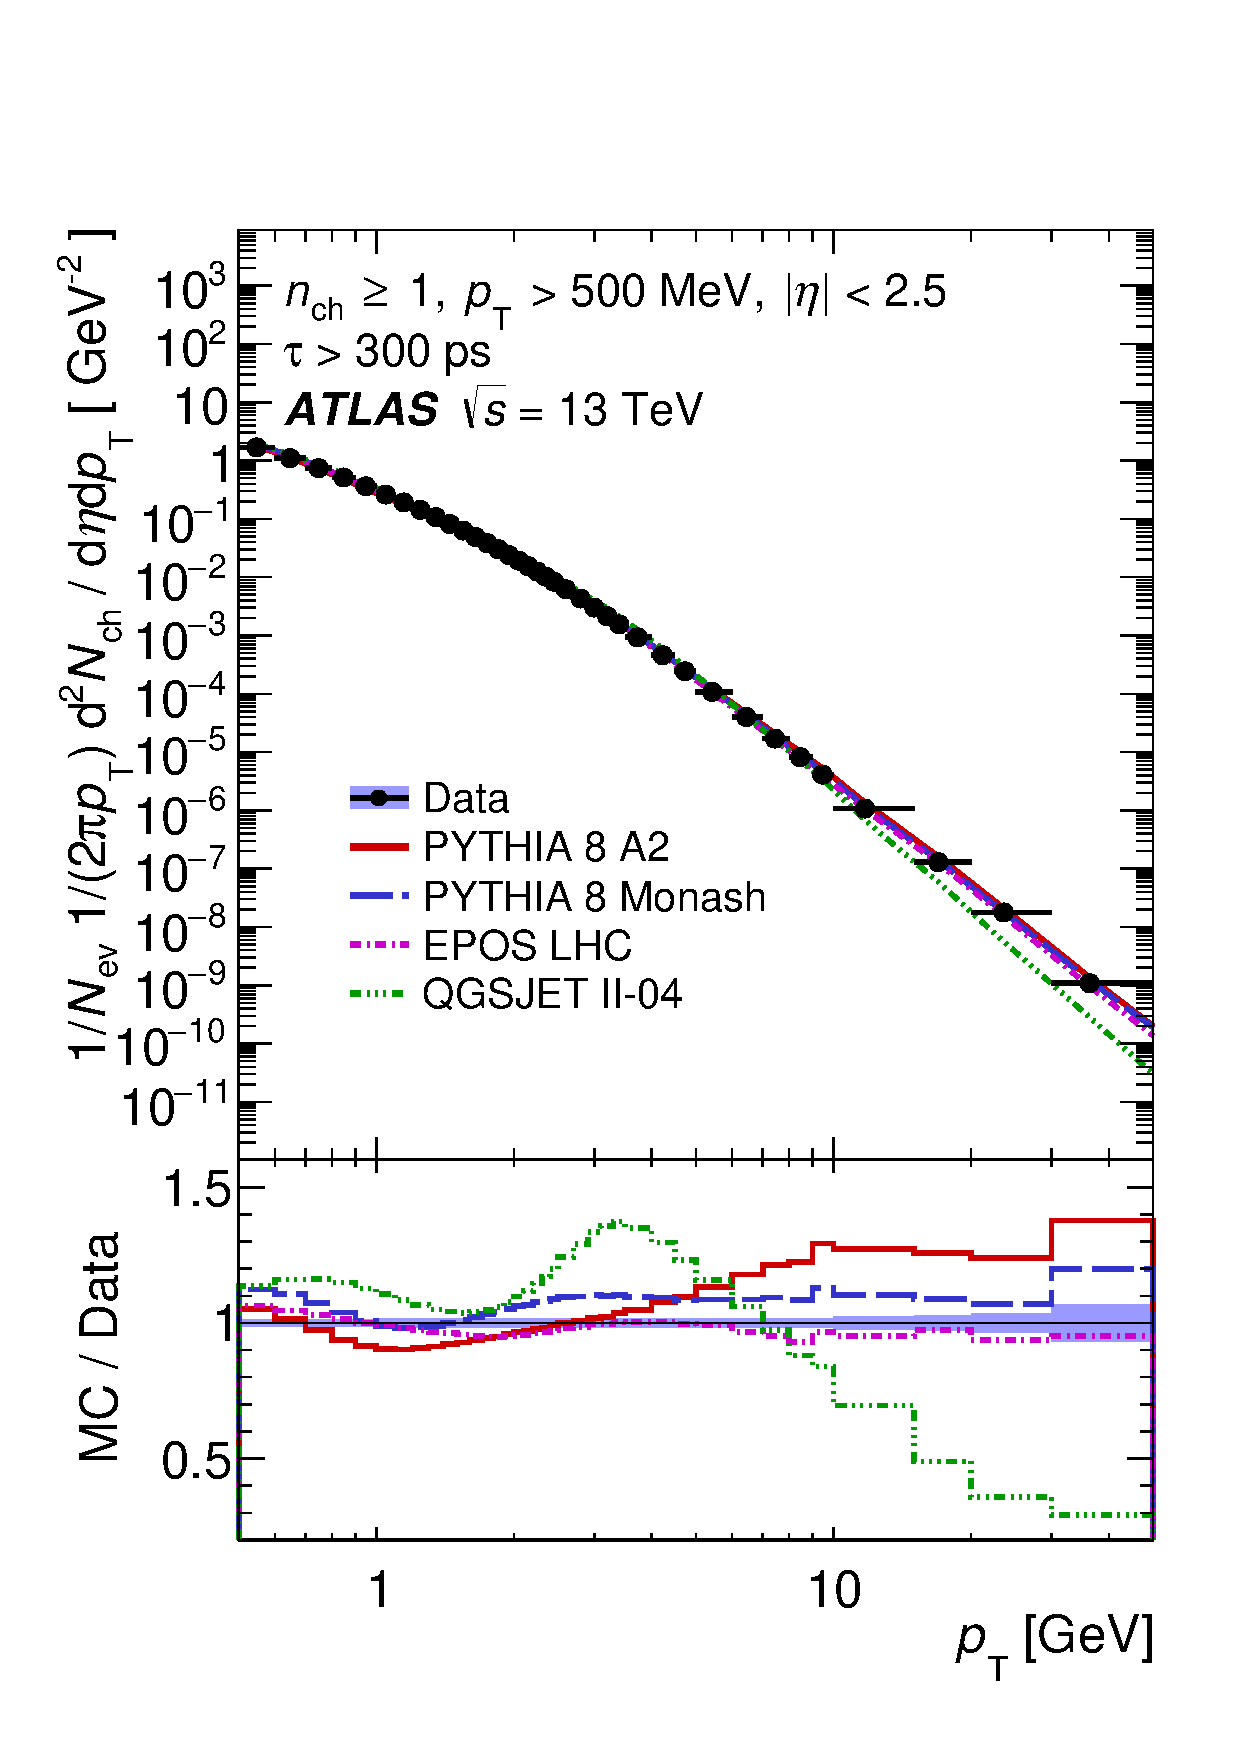
\includegraphics[width=0.55\textwidth]{figures/theory/inclhadronCS}
%\caption{The charged particle multiplicities as a function of transverse momentum \pt\ in \sqrts = 13 TeV \pp\ collisions as measured by ATLAS. The data are compared to NLO pQCD calculations. Taken from \cite{201667}. }
%\label{fig:inclhadronCS}
%\end{center}
%\end{figure}
%
%
%
%Equation~\ref{eq:hadronCS} is written at leading order (LO) and includes contributions from $2\rightarrow2$ cross sections, LO re-summed PDFs and FFs, and single loop expression for the strong coupling \alphas. At next to leading order (NLO), the contributions from real $2\rightarrow3$ and virtual $2\rightarrow3$ processes, as well as the double loop expression for \alphas are included. These calculations describe the inclusive and pQCD, NLO calculations have next to leading order (NLO) calculations that include Figure~\ref{fig:incl_hadron_CS} hows the inclusive jet cross section as measured by ATLAS in \sqrts = 13 TeV \pp\ collisions. 
%
%
%
%
%In a heavy ion collision where the QGP is formed, the hard scattering interactions between the partons strongly interact with the QGP due to their color charge and are modified and lose energy via collisions with the medium constituents, or gluon bremsstrahlung. 

\clearpage

\chapter{MEASUREMENTS IN HEAVY ION COLLISIONS}
\label{sec:jetMeasurements}
% !TEX encoding = UTF-8 Unicode
% !TEX root = thesis-ex.tex
This chapter shall discuss some important experimental jet measurements that motivate the study of the main analysis in this thesis. These include the study of the jet yields, dijet asymmetry, and jet fragmentation. It shall then go on to discuss a few models that have been used to explain the data, looking in particular at the following: Effective Quenching (EQ), Soft Collinear Effective Theory (SCET), Hybrid Model, and Jet Fluid Model.


\section{Dijet Balance: $\mathrm{x}_{J}$}
\label{sec:xj}
This section will discuss the dijet balance for $R = 0.4$ jets as measured by ATLAS detector for \pbpb\ collisions at \sqrtsnn = 2.76 TeV \cite{Aaboud:2017eww}. The dijet imbalance can be expressed in terms of $x_J$ defined as

\begin{align}
x_J =  \frac{\pt_2}{\pt_1}
\end{align}

where $\pt_2$ and $\pt_1$ are the transverse momenta of the two highest-\pt\ jets in the event respectively. The minimum $\pt_2$ considered is 25 GeV and the pair of jets are separated by $|\Delta\phi| > 7\pi/8$. The dijet yields normalized by the number of jets and determined as $1/N_\mathrm{jets} dN/dx_J$ are presented as a function of $x_J$ for different centrality intervals, as well as different ranges for $\pt_1$. The measured distributions are further unfolded to remove detector resolution effects and allow comparison to theoretical models.

Figure~\ref{fig:xJ} shows the $x_J$ distribution for dijet pairs in \pp\ and \pbpb\ collisions in two different centrality bins and two $\pt_1$ ranges. It can be seen that the dijet yields in \pp\ are peaked at unity and become narrower for larger $\pt_1$ ranges. This reflects the fact that the effects of jet quenching are minimal and the higher-\pt\ jets are better balanced. The dijet yields in peripheral \pbpb\ collisions are similar to the distributions from the \pp\ data, showing that the effects of quenching are smaller. On the other hand, dijet yields in central \pbpb\ collisions are significantly broadened, reflecting the maximal  of jet quenching. This is consistent with the picture of the individual jets in the dijet pair traversing different lengths in the QGP and hence losing different amounts of energy. In fact, the distribution for \pbpb\ data is peaked at $x_J = 0.5$, implying a loss of 50\% of the jet \pt.

\begin{figure}[htbp]
\begin{center}
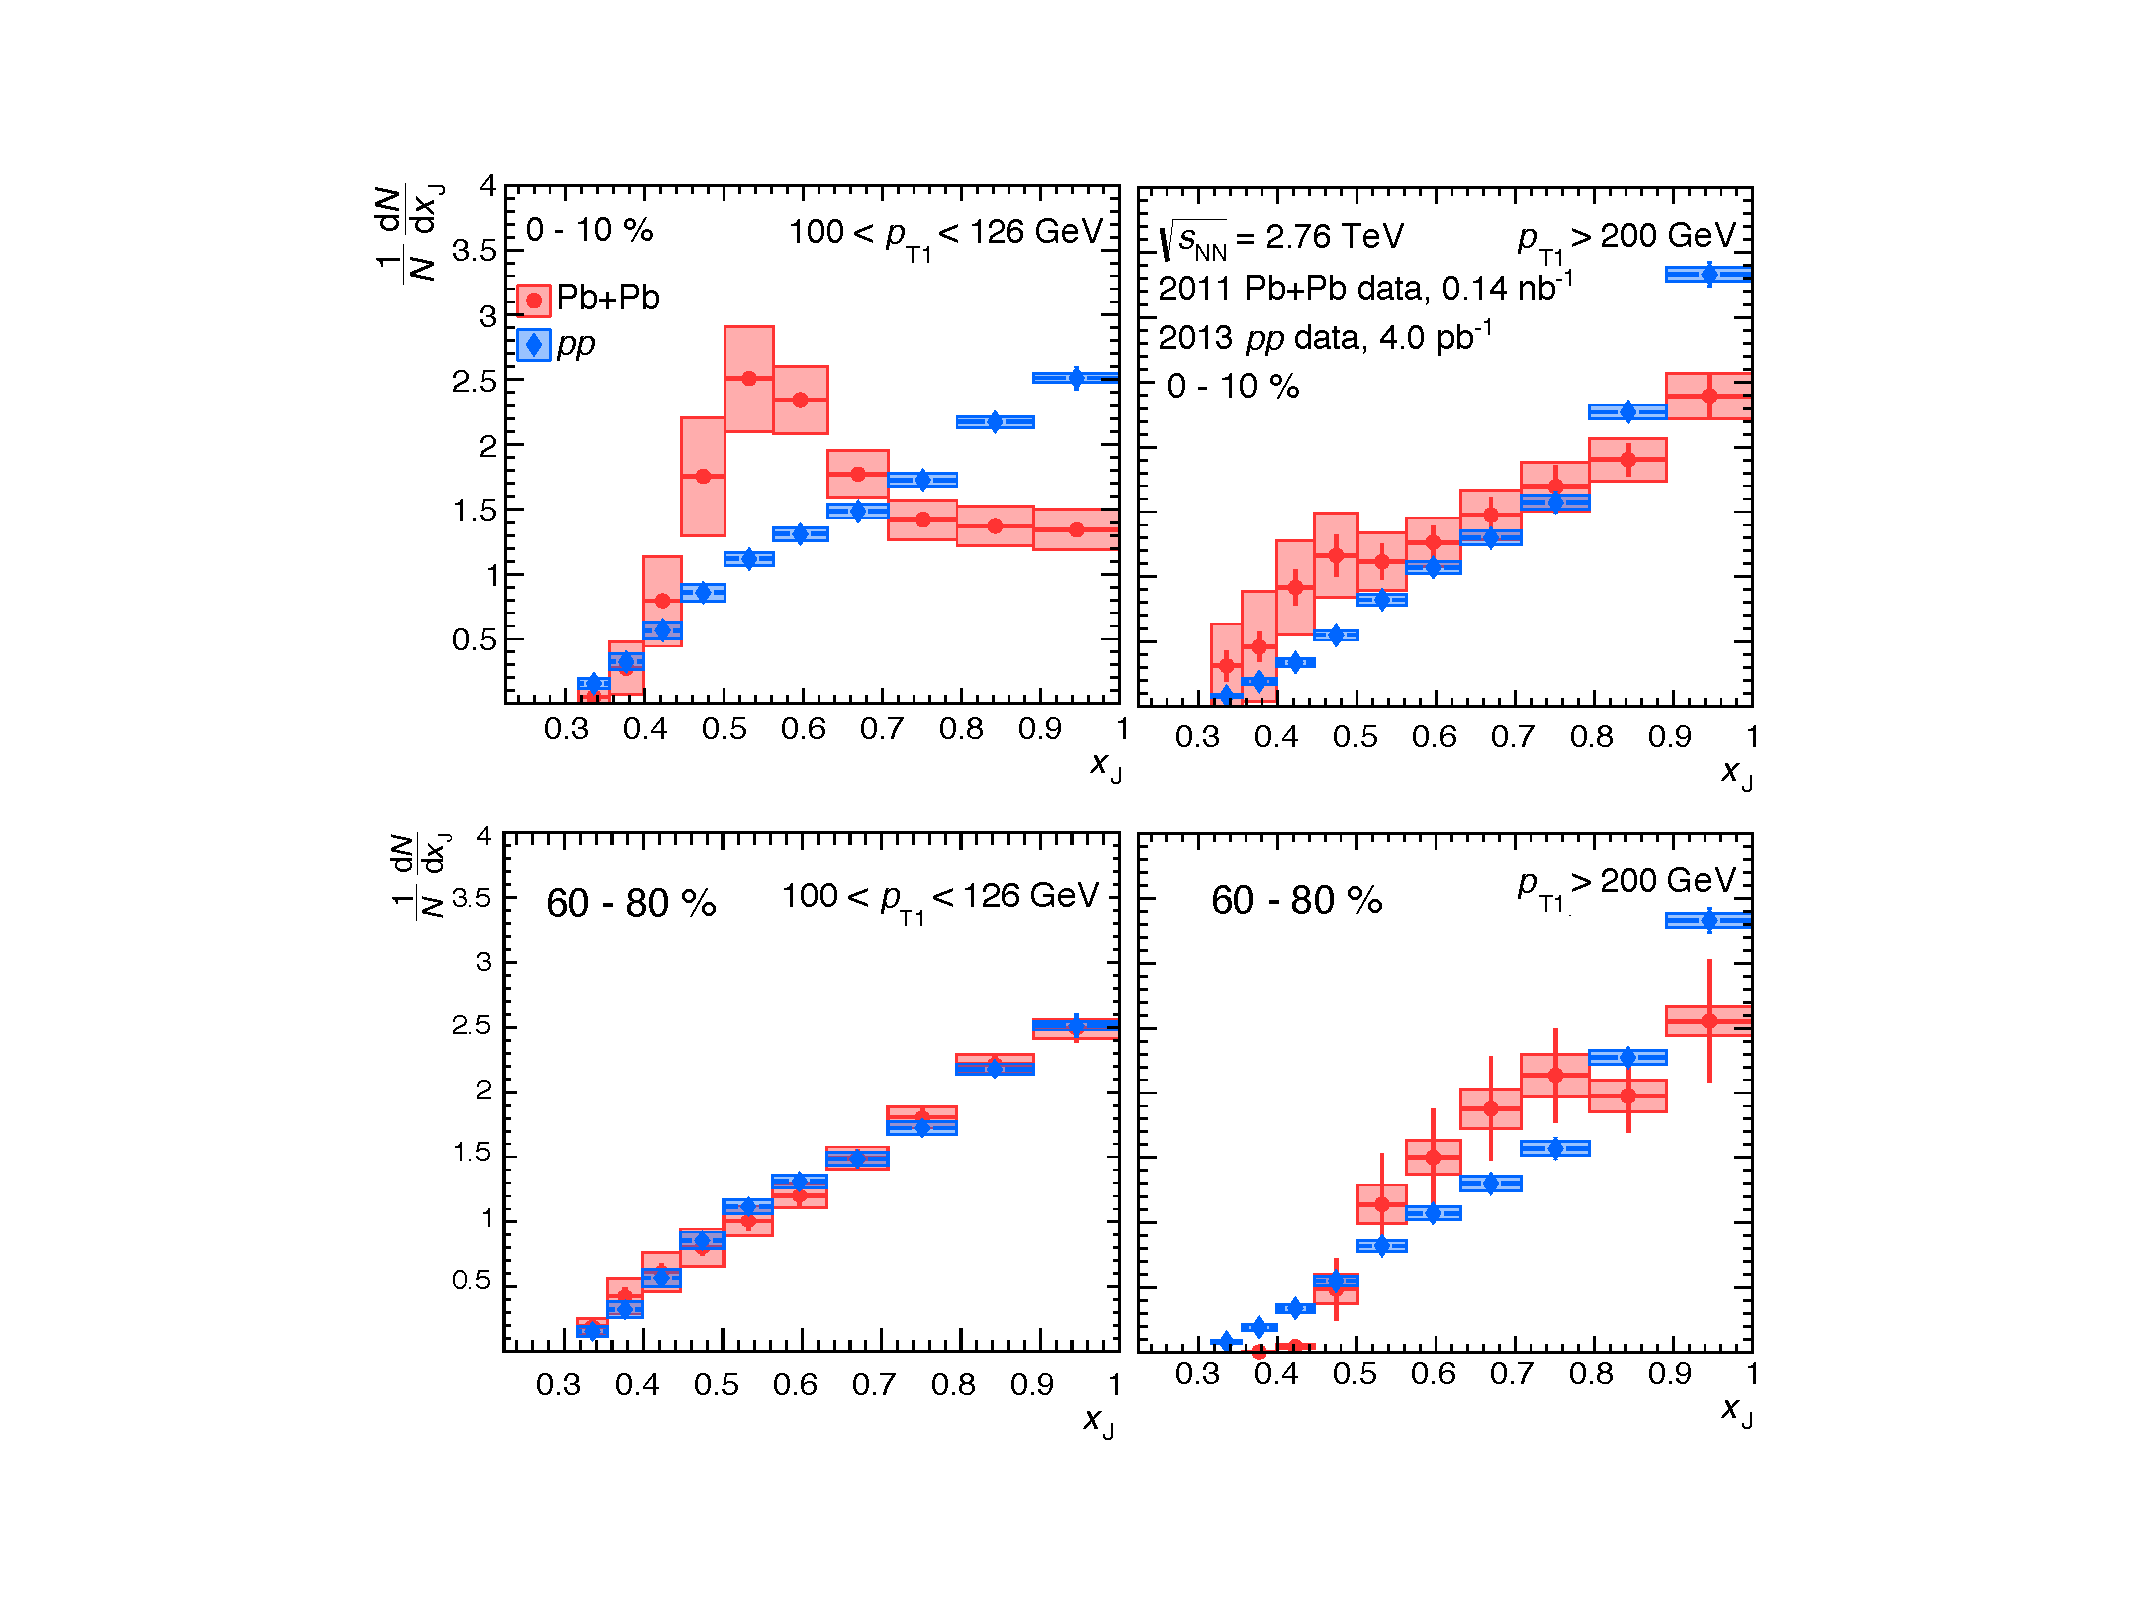
\includegraphics[width=0.55\textwidth]{figures/jetMeasurements/xJ}
\caption{The $1/N_\mathrm{jets} dN/dx_J$ distributions for $R=0.4$ jets as a function of $x_J$ for \pp\ (blue) and \pbpb\ (red) collisions. The different panels are for (top) central and (bottom) peripheral collisions in (left) $100 < \pt_1 < 126$ GeV and (right) $\pt_1 > 200 $ GeV. The \pp\ data is the same in all panels. The statistical uncertainties are indicated by the bars while the boxes indicate the systematic uncertainties. Figures taken from \cite{Aaboud:2017eww}.}
\label{fig:xJ}
\end{center}
\end{figure}

Further measurements of $R = 0.3$ jets are shown in Figure~\ref{fig:xJ_R03}. These distributions are significantly flatter than the ones for $R=0.4$ jets, an observation that is consistent with the expectation that the transverse momenta correlation between the dijet pair is weaker for jets with smaller radii due to radiation that is outside the nominal jet cone.

\begin{figure}[htbp]
\begin{center}
\includegraphics[width=0.55\textwidth]{figures/jetMeasurements/xJ_R03}
\caption{The $1/N_\mathrm{jets} dN/dx_J$ distributions for $R=0.3$ jets as a function of $x_J$ in \pp\ and central \pbpb\ collisions. The different panels are for different, $\pt_1$ ranges (top left to bottom right) central and (bottom) peripheral collisions. The \pbpb\ data is in red circles while the \pp\ data is in blue diamonds and is the same in all panels. The statistical uncertainties are indicated by the bars while the boxes indicate the systematic uncertainties. Figures taken from \cite{Aaboud:2017eww}.}
\label{fig:xJ_R03}
\end{center}
\end{figure}

%%%%%%%%%%%%%%%%%%%%%%%%%%%%%%%%%%%%%%
\section{Modification of jet yields: $\mathrm{R}_{AA}$}
\label{sec:jet_raa}

This section discusses the measurement of the inclusive jet \RAA\ as measured by the ATLAS detector for $R=0.4$ jets in $\sqrtsnn=5.02$ TeV \pbpb\ collisions \cite{2019108}.

While a measurement that compares the jets in a dijet system to each other as discussed in Section~\ref{sec:xj} can provide valuable information about how jets lose energy, it has the following limitation: If both jets lose equal amounts of energy, the dijet yield will still be peaked at unity and no new information will be obtained. Thus, it is useful to compare the jet yields directly between the \pp\ and \pbpb\ systems and construct the jet \RAA\ observable. This is defined as:

\begin{align}
\RAA  = \dfrac{\dfrac{1}{N_{\rm evt}} \left. \dfrac{d^2 N_{\rm jet}}{d\pt dy} \right|_{\rm cent}}{ \langle T_{\rm AA} \rangle \left. \dfrac{d^2\sigma_{\rm jet}}{d\pt dy} \right|_{\rm pp}}
\end{align}

where \TAA\ is the nuclear thickness function and accounts for the geometric enhancement between \pp\ and \pbpb\ as discussed in Section~\ref{sec:HICollisions} and \cite{doi:10.1146/annurev.nucl.57.090506.123020}. 

This measurement was conducted for jets in the 40--1000 GeV range in different rapidity and centrality intervals. The jet yields in \pp\ and \pbpb\ collisions are shown in Figure~\ref{fig:jet_yields} . The \pbpb\ jet yields are scaled by the thickness function and are shown for 8 centrality intervals. 

\begin{figure}[htbp]
\begin{center}
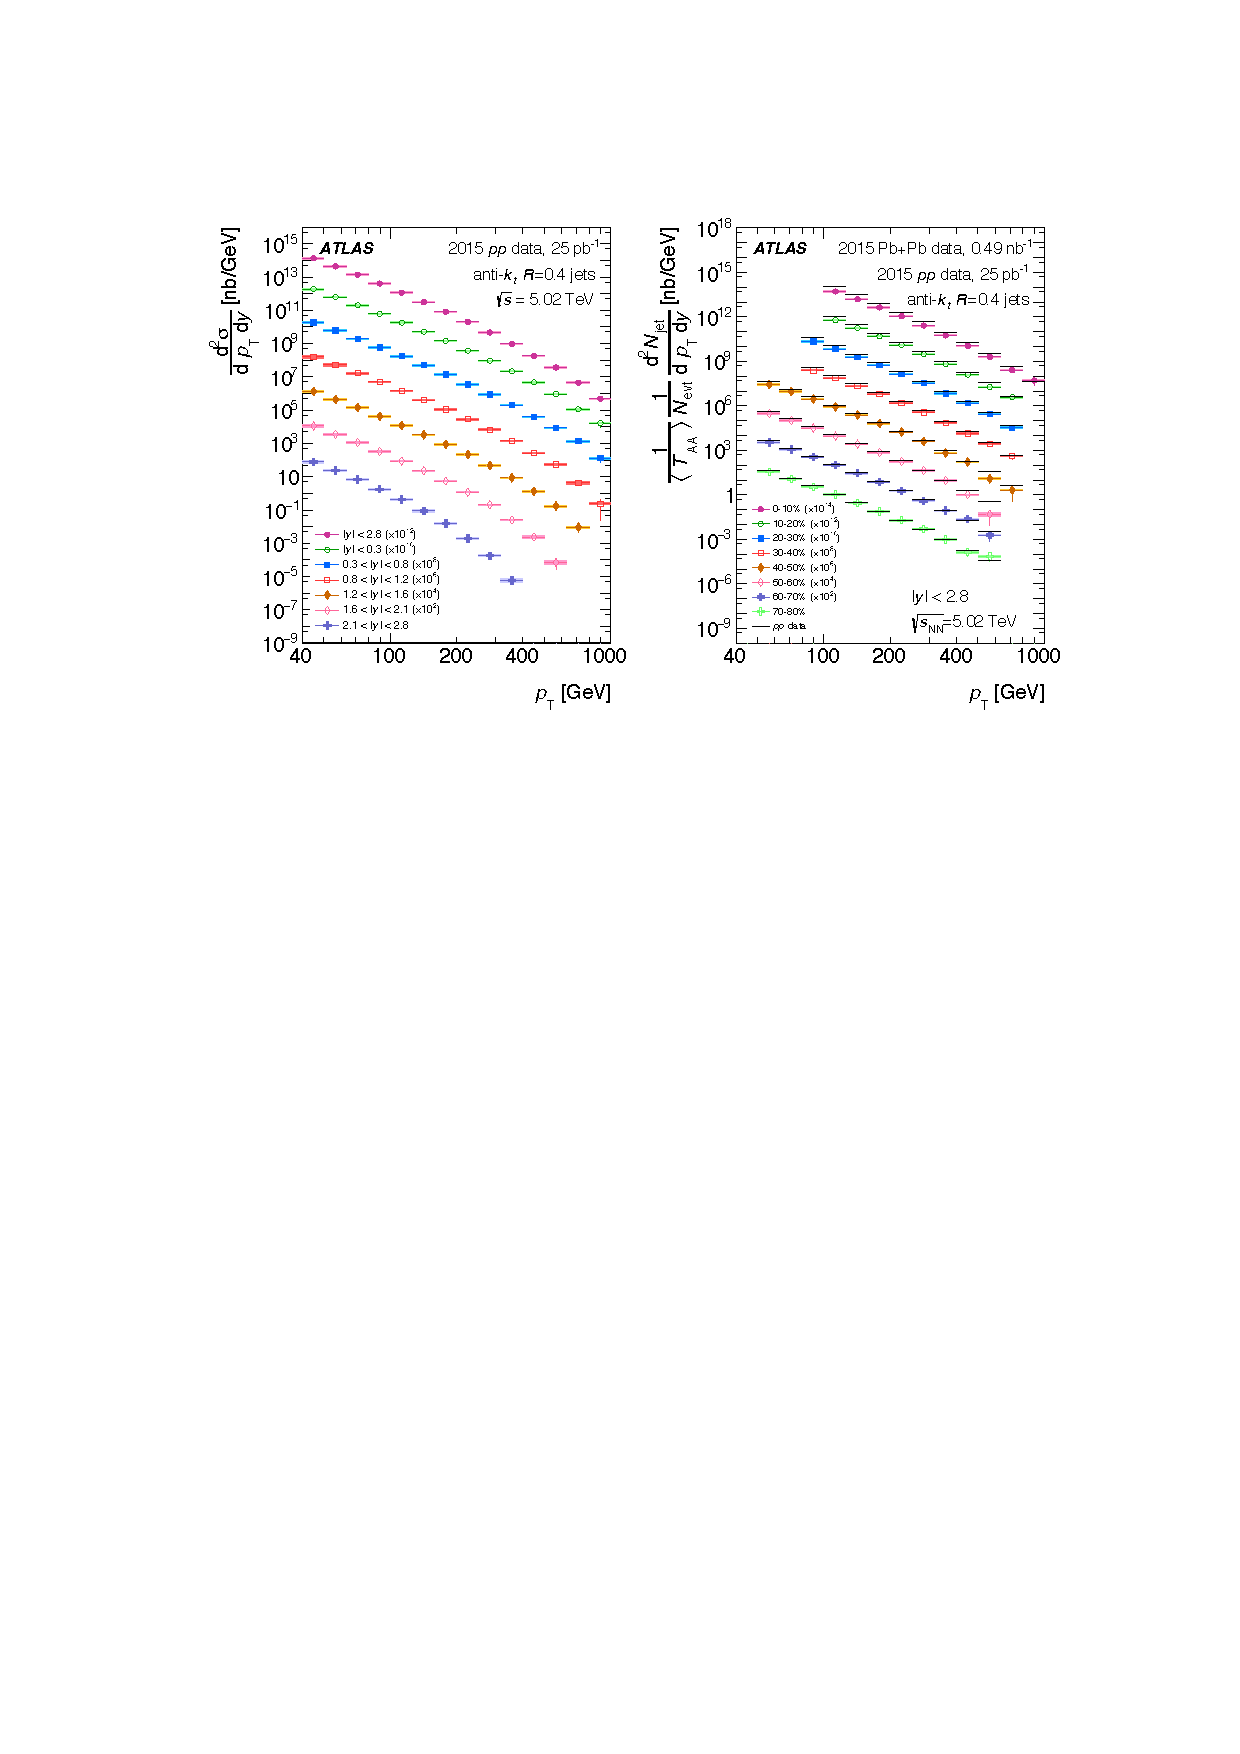
\includegraphics[width=0.85\textwidth]{figures/jetMeasurements/jetYields}
\caption{(Left) The inclusive jet cross section in \pp\ collisions as a function of jet \pt\ in different $|y|$ intervals scaled by successive powers of $10^2$ for visibility. (Right) Per event inclusive jet yield in \pbpb\ collisions normalized by $\langle \TAA \rangle$ as a function of jet \pt\ in different centrality intervals scaled by successive powers of $10^2$ for visibility. The solid lines represent the cross section from \pp\ data at the same rapidity interval scaled by the same $10^2$ factor.  Figure taken from \cite{2019108}.}
\label{fig:jet_yields}
\end{center}
\end{figure}


Figure~\ref{fig:raa} shows the measured inclusive jet \RAA\ as a function of jet \pt\ for different centrality bins and jet rapidity $|y| < 2.8$. It can be seen that the most central collisions show a clear suppression with an $\RAA \approx 0.45$ at jet $\pt\ 100$ GeV. The \RAA\ value slowly evolves with jet \pt\ and rises to 0.6 at jet $\pt = 800$ GeV. This modification becomes smaller for more peripheral collisions. 

\begin{figure}[htbp]
\begin{center}
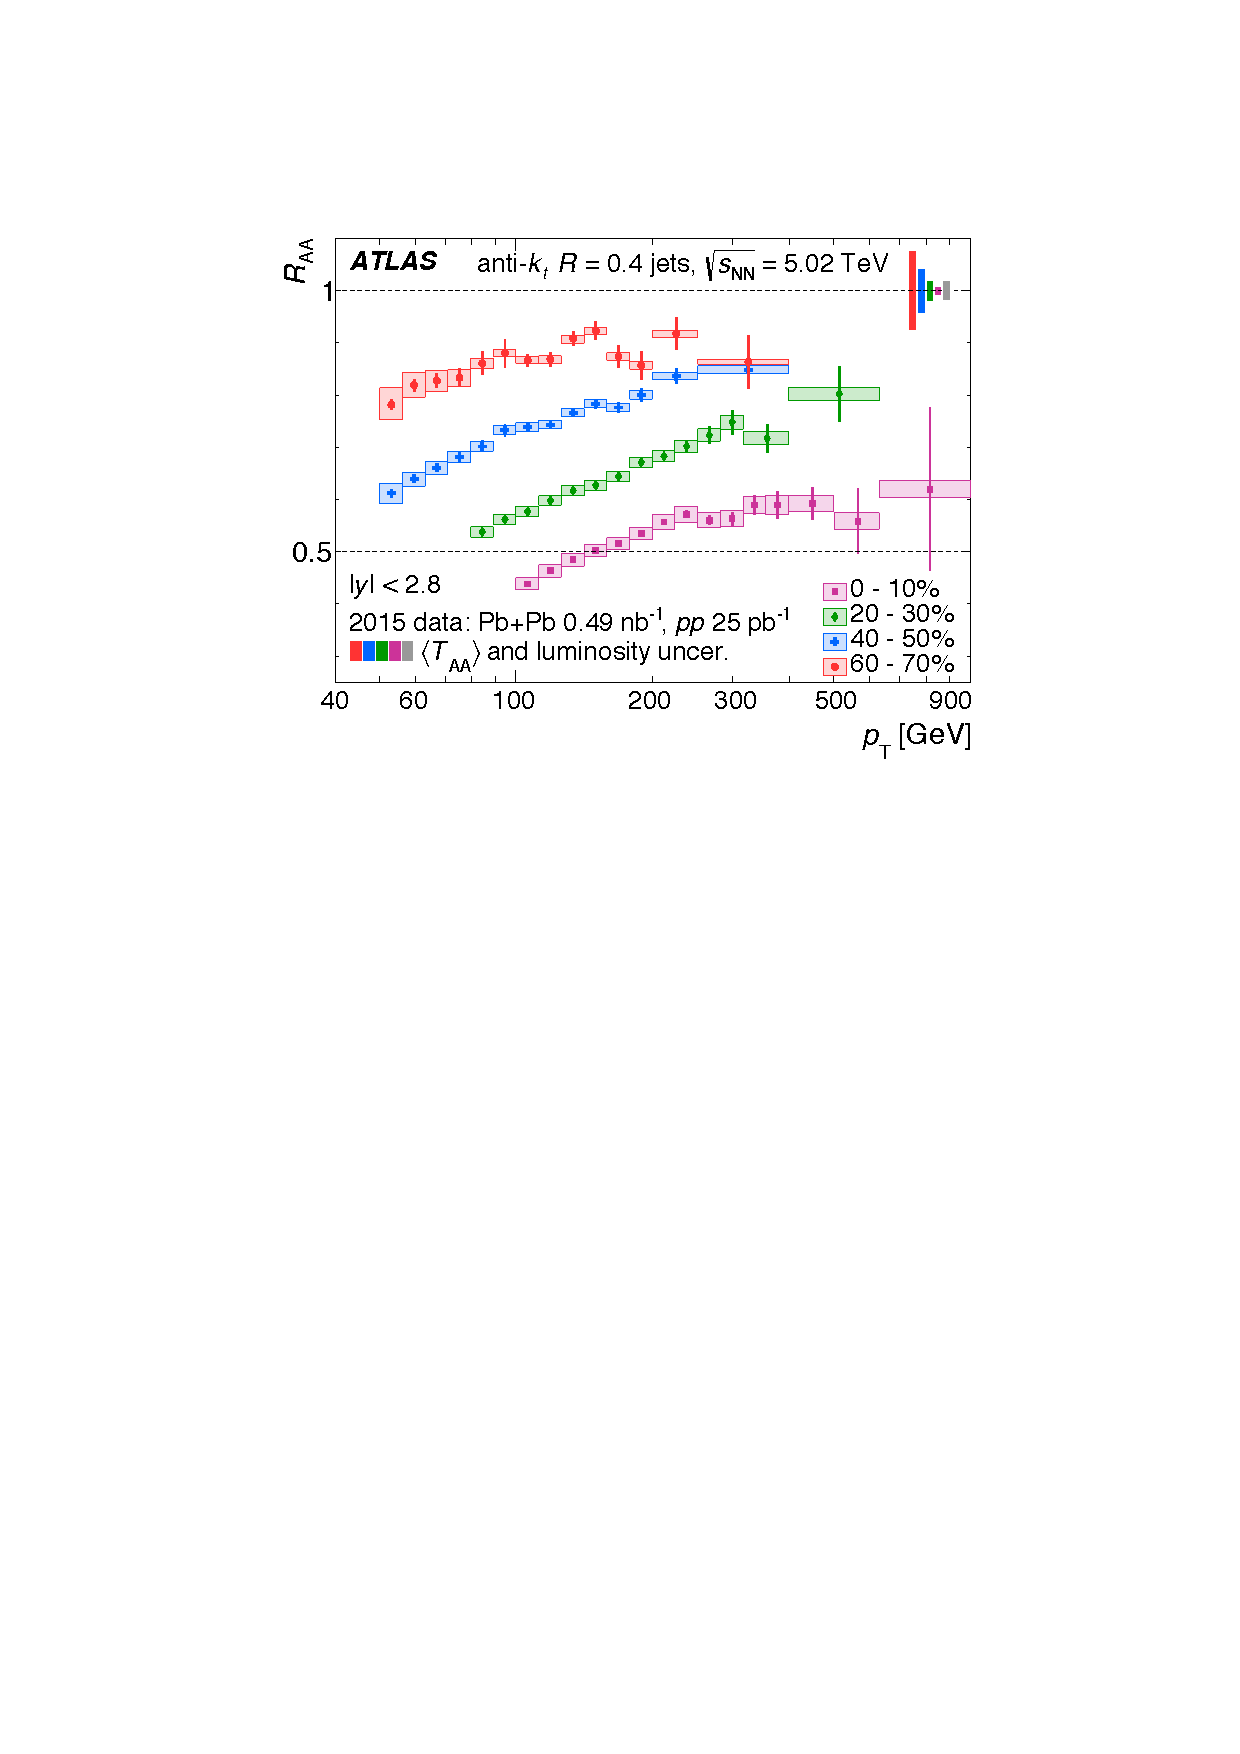
\includegraphics[width=0.55\textwidth]{figures/jetMeasurements/raa}
\caption{The \RAA\ distributions as a function of jet \pt\ for different centrality bins and jet rapidity $|y| < 2.8$. The error bars represent statistical uncertainties while the shaded boxes represent systematic uncertainties. Figure taken from \cite{2019108}.}
\label{fig:raa}
\end{center}
\end{figure}

The smooth centrality dependence can be more clearly seen in Figure~\ref{fig:raa_centDep}, where \RAA\ is shown as a function of \ANpart\ for jets the 100--126 GeV and 200--251 GeV ranges. The magnitude of the suppression is also seen to significantly depend on jet \pt\ for $\ANpart \geq 50$. 

\begin{figure}[htbp]
\begin{center}
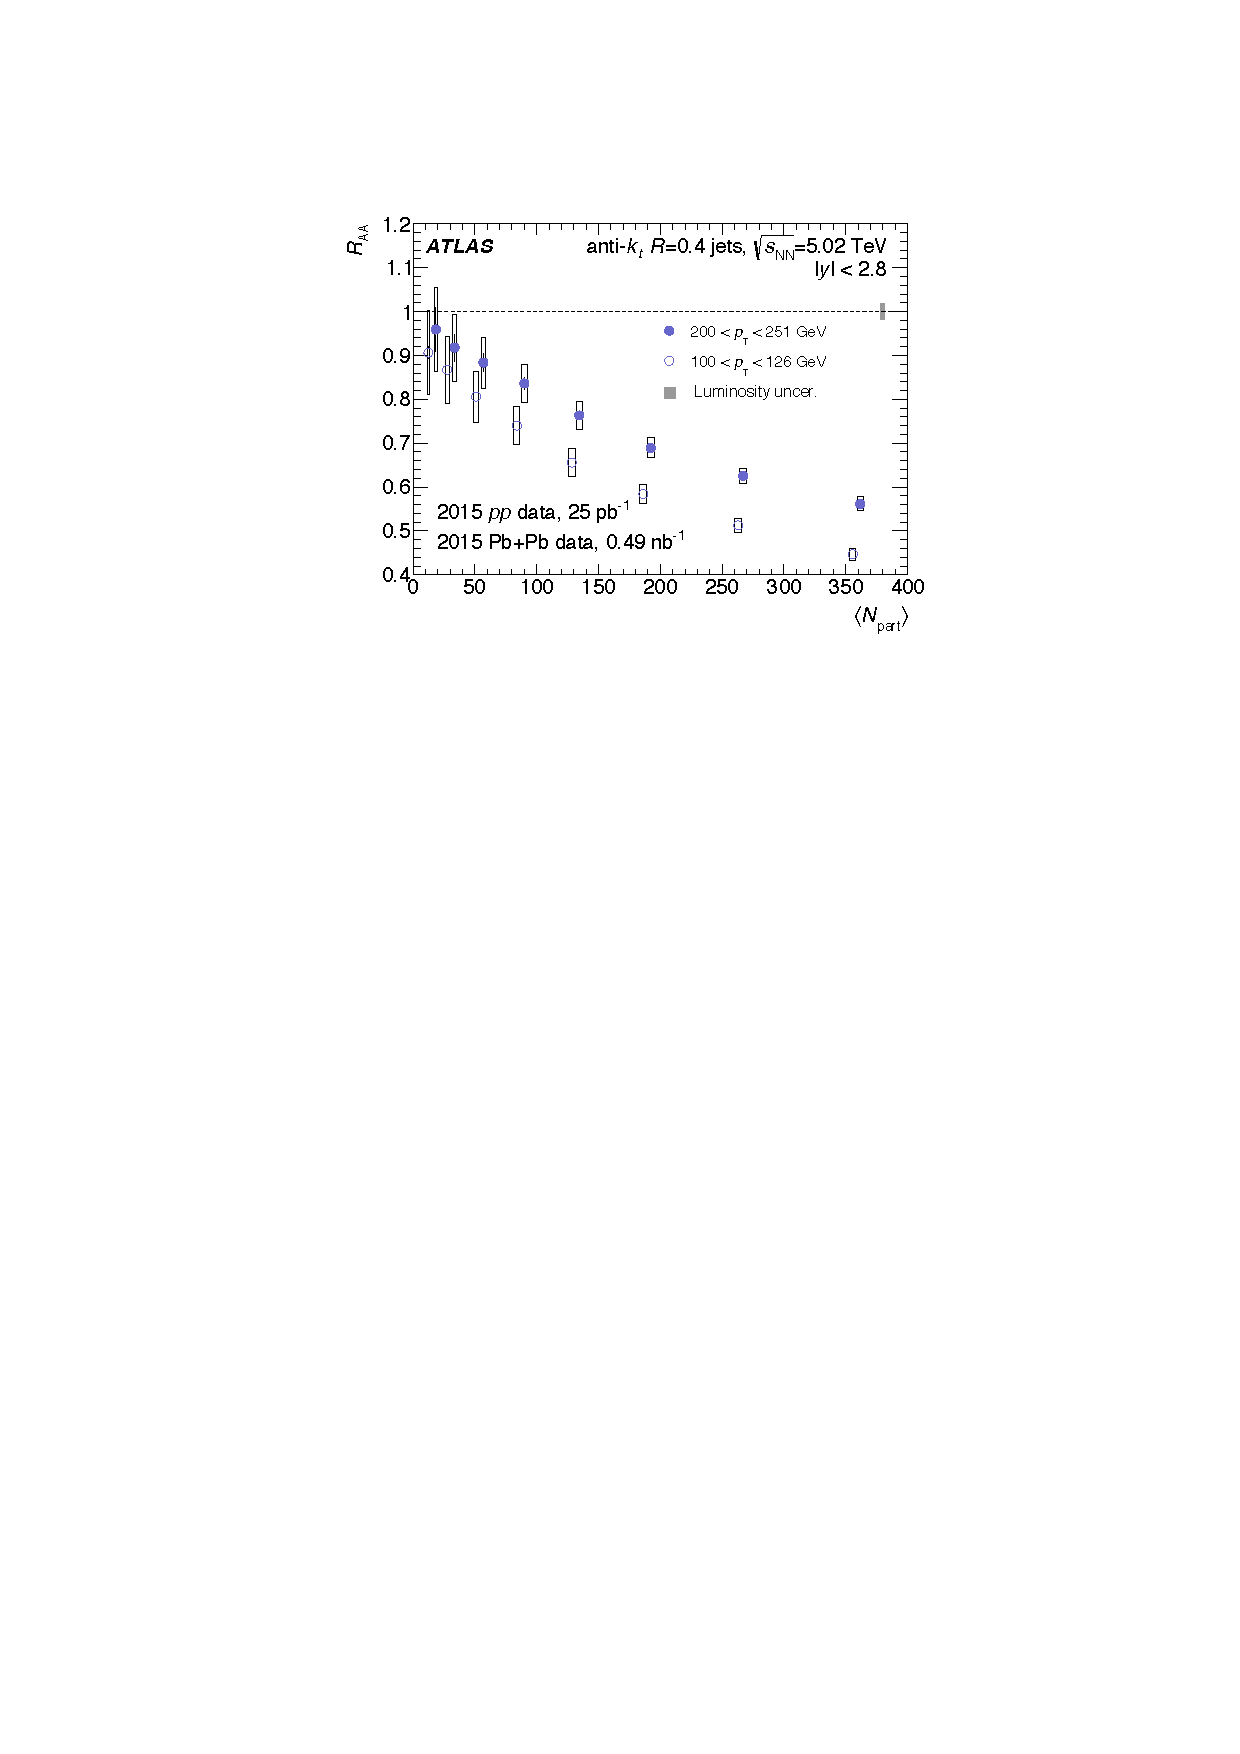
\includegraphics[width=0.55\textwidth]{figures/jetMeasurements/raa_centDep}
\caption{The \RAA\ distributions as a function of jet \pt\ for different centrality bins and jet rapidity $|y| < 2.8$. The error bars represent statistical uncertainties while the shaded boxes represent systematic uncertainties. Figure taken from \cite{2019108}.}
\label{fig:raa_centDep}
\end{center}
\end{figure}

%The measurement further looked at the $y$ dependence of \RAA\ as described by $\RAA (|y|) / \RAA (|y| < 0.3)$. This is useful because it is sensitive to the different quark to gluon fractions at different rapidities.  the uncertainties largely cancel, an













%%%%%%%%%%%%%%%%%%%%%%%%%%%%%%%%%%%%%%
\section{Jet Fragmentation}
\label{sec:jet_ff}
This discussion is based on the measurement described in \cite{PhysRevC.98.024908}. While measurements like \RAA \cite{} and asymmetry \cite{} describe how much energy is lost by the jet, fragmentation measurements describe the momentum distribution of particles associated to the jet. These can be described as:

\begin{align}
\Dz = \frac{1}{\Njet} \frac{d\nch}{dz} \\
\Dpt = \frac{1}{\Njet} \frac{d\nch}{d\pt}
\end{align}
where $z = \pt \cos(\Delta R / \ptjet)$ and gives the charged-particle longitudinal momentum fraction relative to the jet. Modifications to the fragmentation functions in \pbpb\ collisions can be evaluated by constructing the ratios: 

\begin{align}
\Rdz = \frac{\Dz_{\pbpb}}{\Dz_{\pp}} \\
\Rdpt = \frac{\Dpt_{\pbpb}}{\Dpt_{\pp}} 
\end{align}
This measurement is corrected for detector effects and unfolded to the particle level. This allows for comparisons to other measurements and theoretical models. The \Dz\ and \Dpt\ distributions are shown in Figure~\ref{fig:jetff_dz} and Figure~\ref{fig:jetff_dpt} 

\begin{figure}[htbp]
\begin{center}
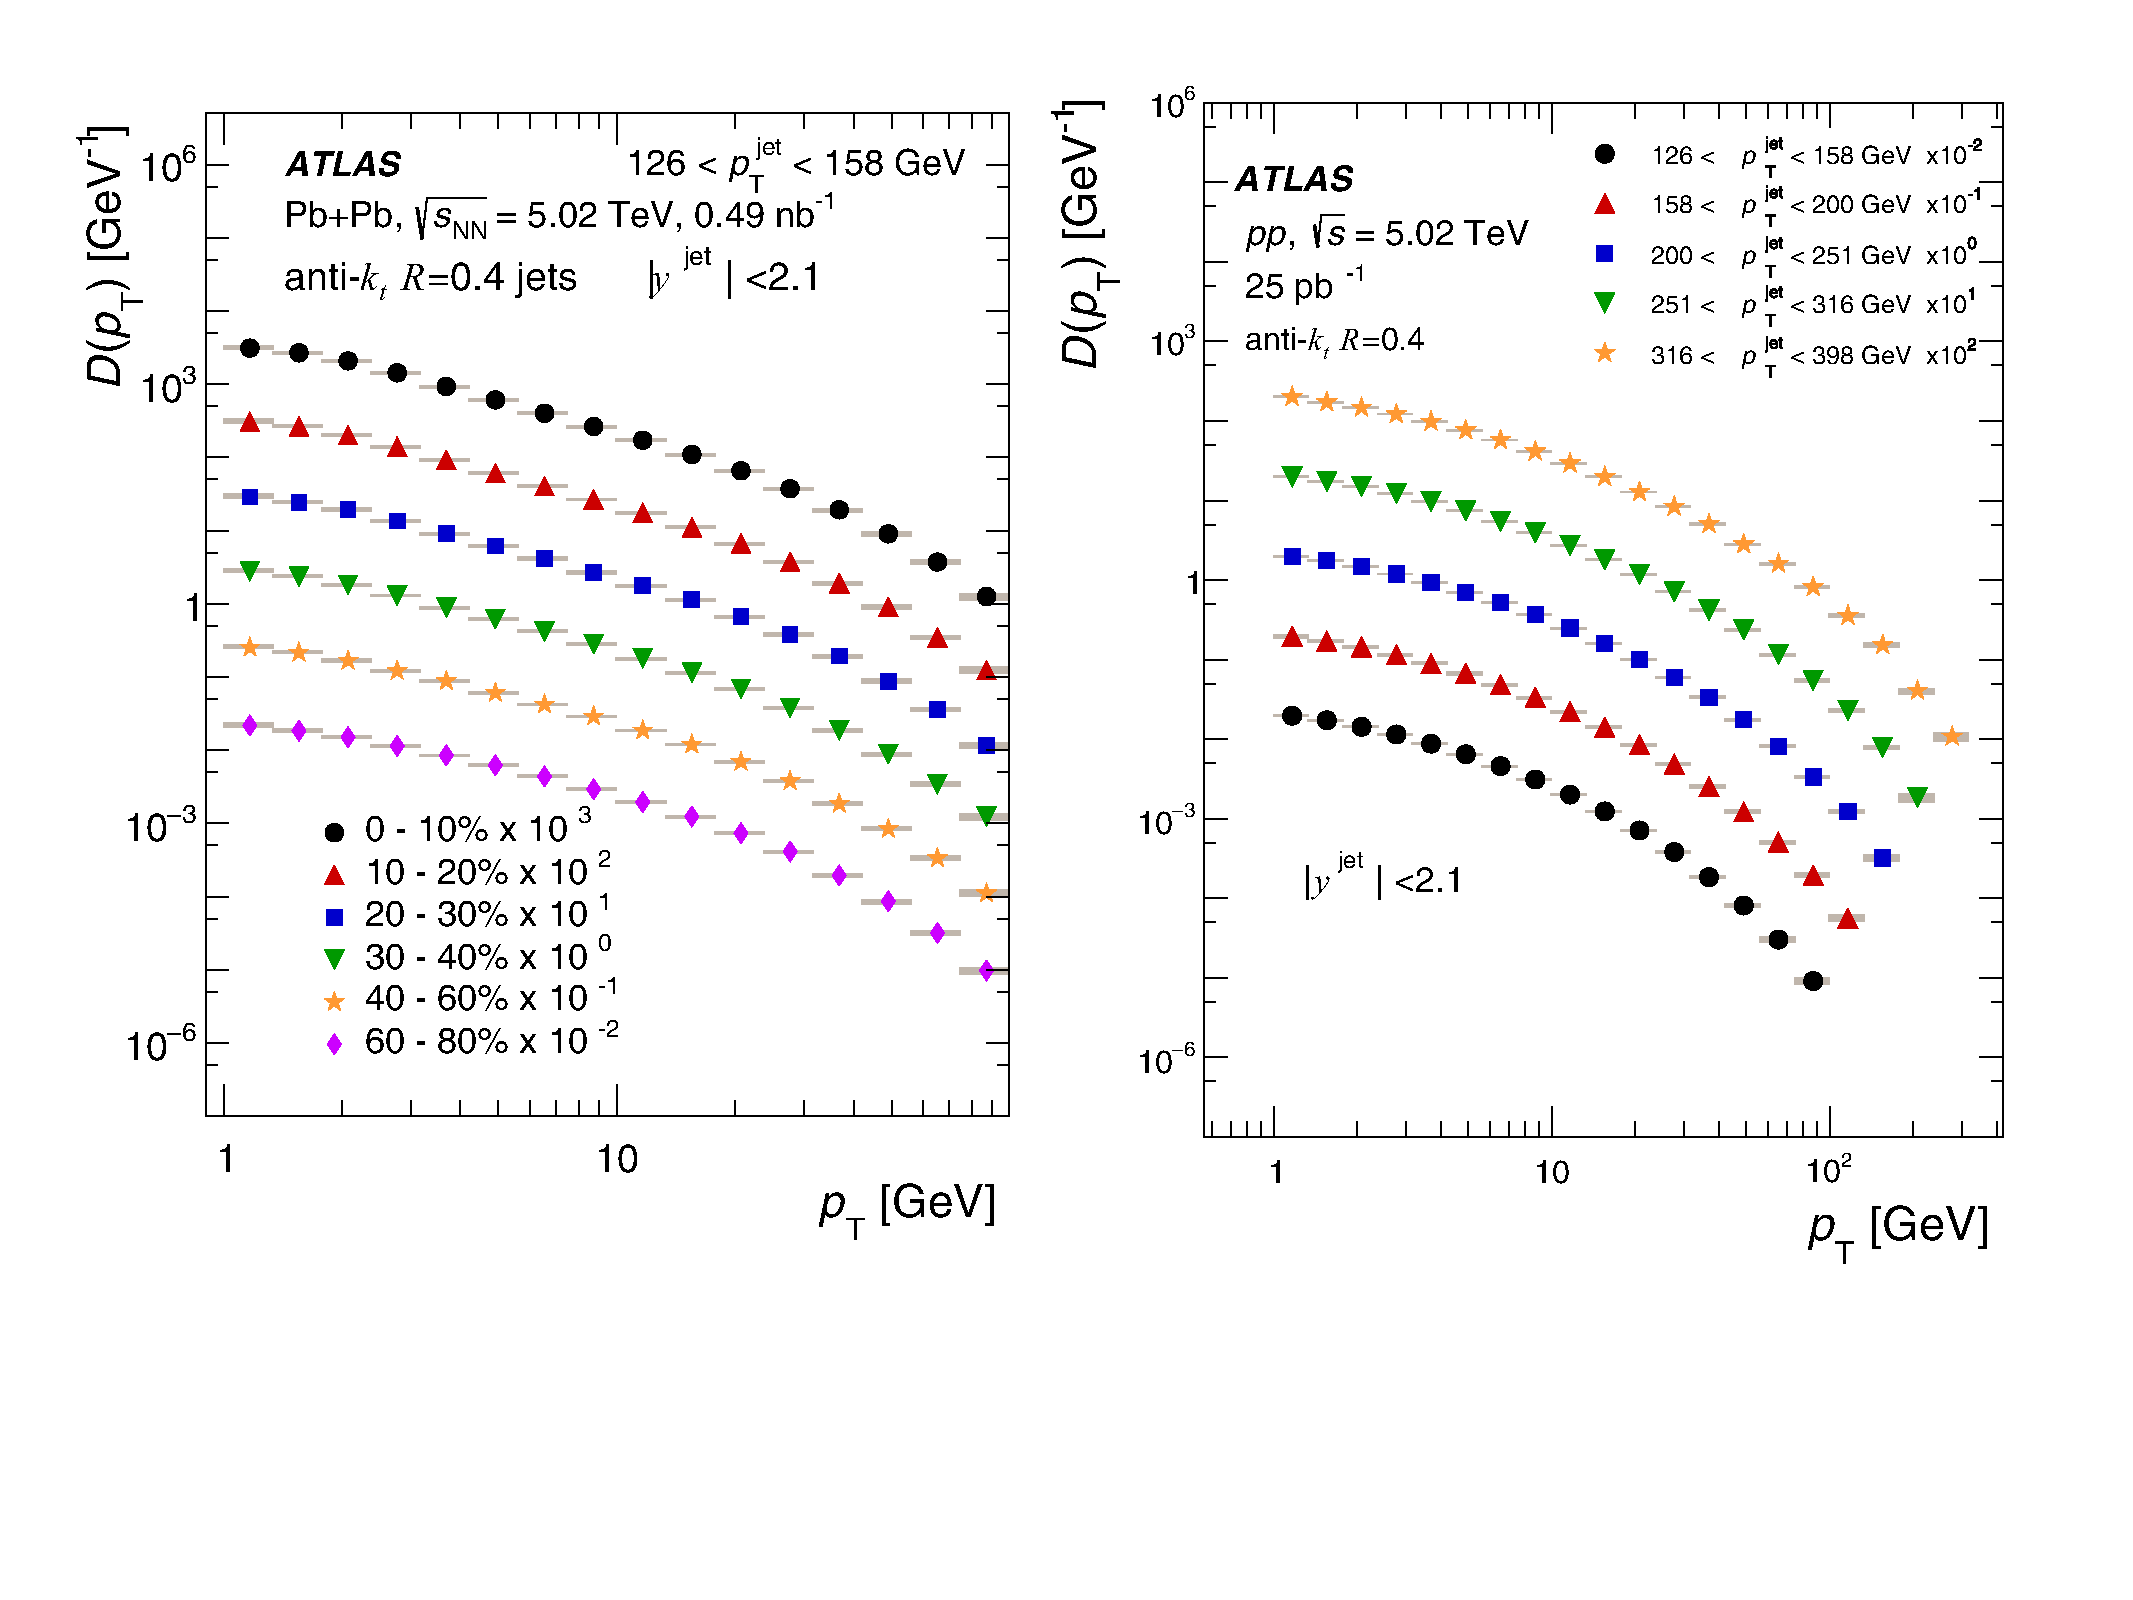
\includegraphics[width=0.55\textwidth]{figures/jetMeasurements/jetff_dpt}
\caption{(Left) The \Dpt\ distributions in \pp\ as a function of charged-particle \pt\ for different \ptjet\ selections and for jet rapidity $|y| < 2.1$. (Right) The \Dpt\ distributions in \pbpb\ as a function of charged-particle \pt\ for different centrality selections and for jet rapidity $|y| < 2.1$. The error bars represent statistical uncertainties while the shaded boxes represent systematic uncertainties. Figure taken from \cite{PhysRevC.98.024908}.}
\label{fig:jetff_dpt}
\end{center}
\end{figure}


\begin{figure}[htbp]
\begin{center}
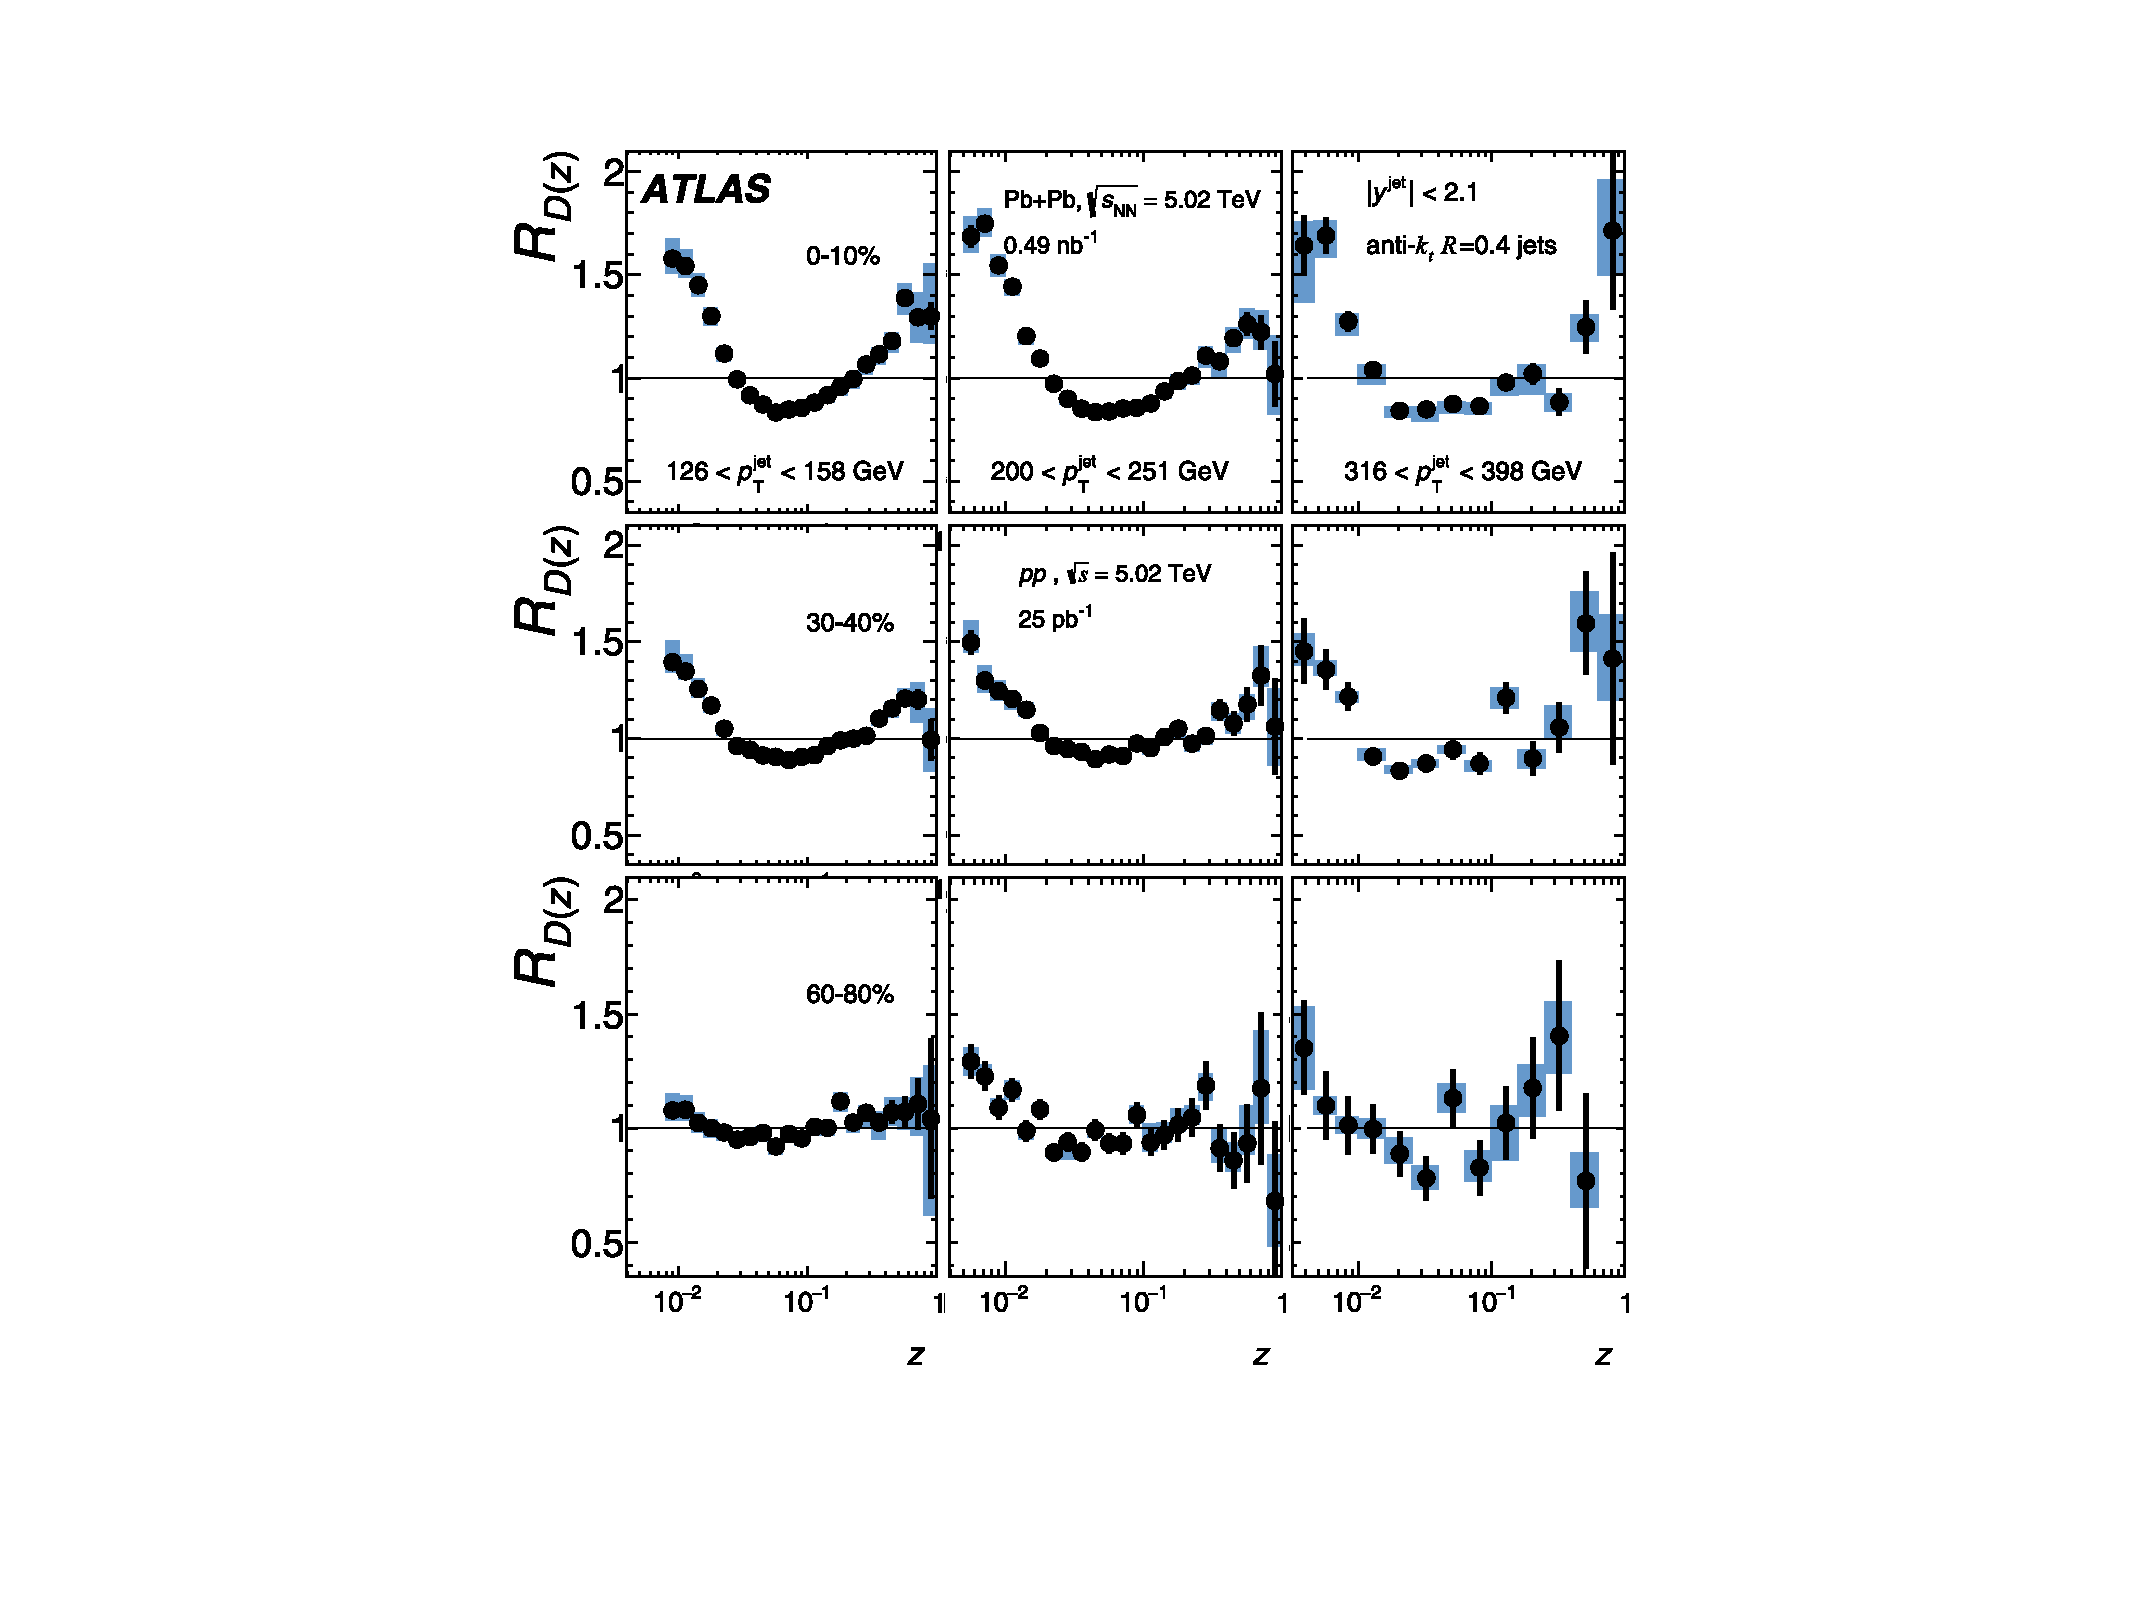
\includegraphics[width=0.55\textwidth]{figures/jetMeasurements/jetff_rdz}
\caption{The modifications to the \Dz\ distributions in \pbpb\ compared to \pp\ as a function of charged-particle $z$ for different \ptjet\ selections (left to right) and different centrality selections (top to bottom) for jet rapidity $|y| < 0.3$. The error bars represent statistical uncertainties while the shaded boxes represent systematic uncertainties. Figure taken from \cite{PhysRevC.98.024908}.}
\label{fig:jetff_rdz}
\end{center}
\end{figure}

The modifications to the \Dz\ distributions are shown in Figure~\ref{fig:jetff_rdz}. It can be seen that there is an excess of particles with low $z$ and high $z$. These are particles that carry either a small or a large fraction of energy of the jet \pt. There is an associated depletion for particles with intermediate $z$. These modifications become smaller for more peripheral collisions. The \ptjet\ dependence of the \Rdz\ and \Rdpt\ distributions can be seen in Figure~\ref{fig:jetff_jetpt_dep}. This dependence can give insight into the modification of the fragmentation functions, with any scaling with $z$ indicating a change in the fragmentation pattern, while a scaling with \pt\ reflecting an effect from the medium itself. The low momentum excess in the \Rdpt\ distributions seen in Figure~\ref{fig:jetff_jetpt_dep} can be further studied by integrating over that region. Then the extra number of particles in \pbpb\ compared to \pp\ is given by:

\begin{align}
\Nch = \int^{\pt_{\mathrm{max}}}_{\pt_{\mathrm{min}}} \left( \Dpt_{\pbpb} - \Dpt_{\pp} \right) d\pt
\end{align}
where $\pt_{\mathrm{min}} = 1$ GeV and $\pt_{\mathrm{max}} = 4.2$ GeV. The \Nch\ distributions can be seen in Figure~\ref{fig:jetff_nch}. It can be clearly seen that the size of the excess increases as a function of \ptjet, growing from about 1.5 to 2.5 extra particles in the most central \pbpb\ collisions. This excess is even seen in the peripheral \pbpb\ collisions, though it is a lot smaller and ranges from 0.2 to 0.5 extra particles. 



\begin{figure}[htbp]
\begin{center}
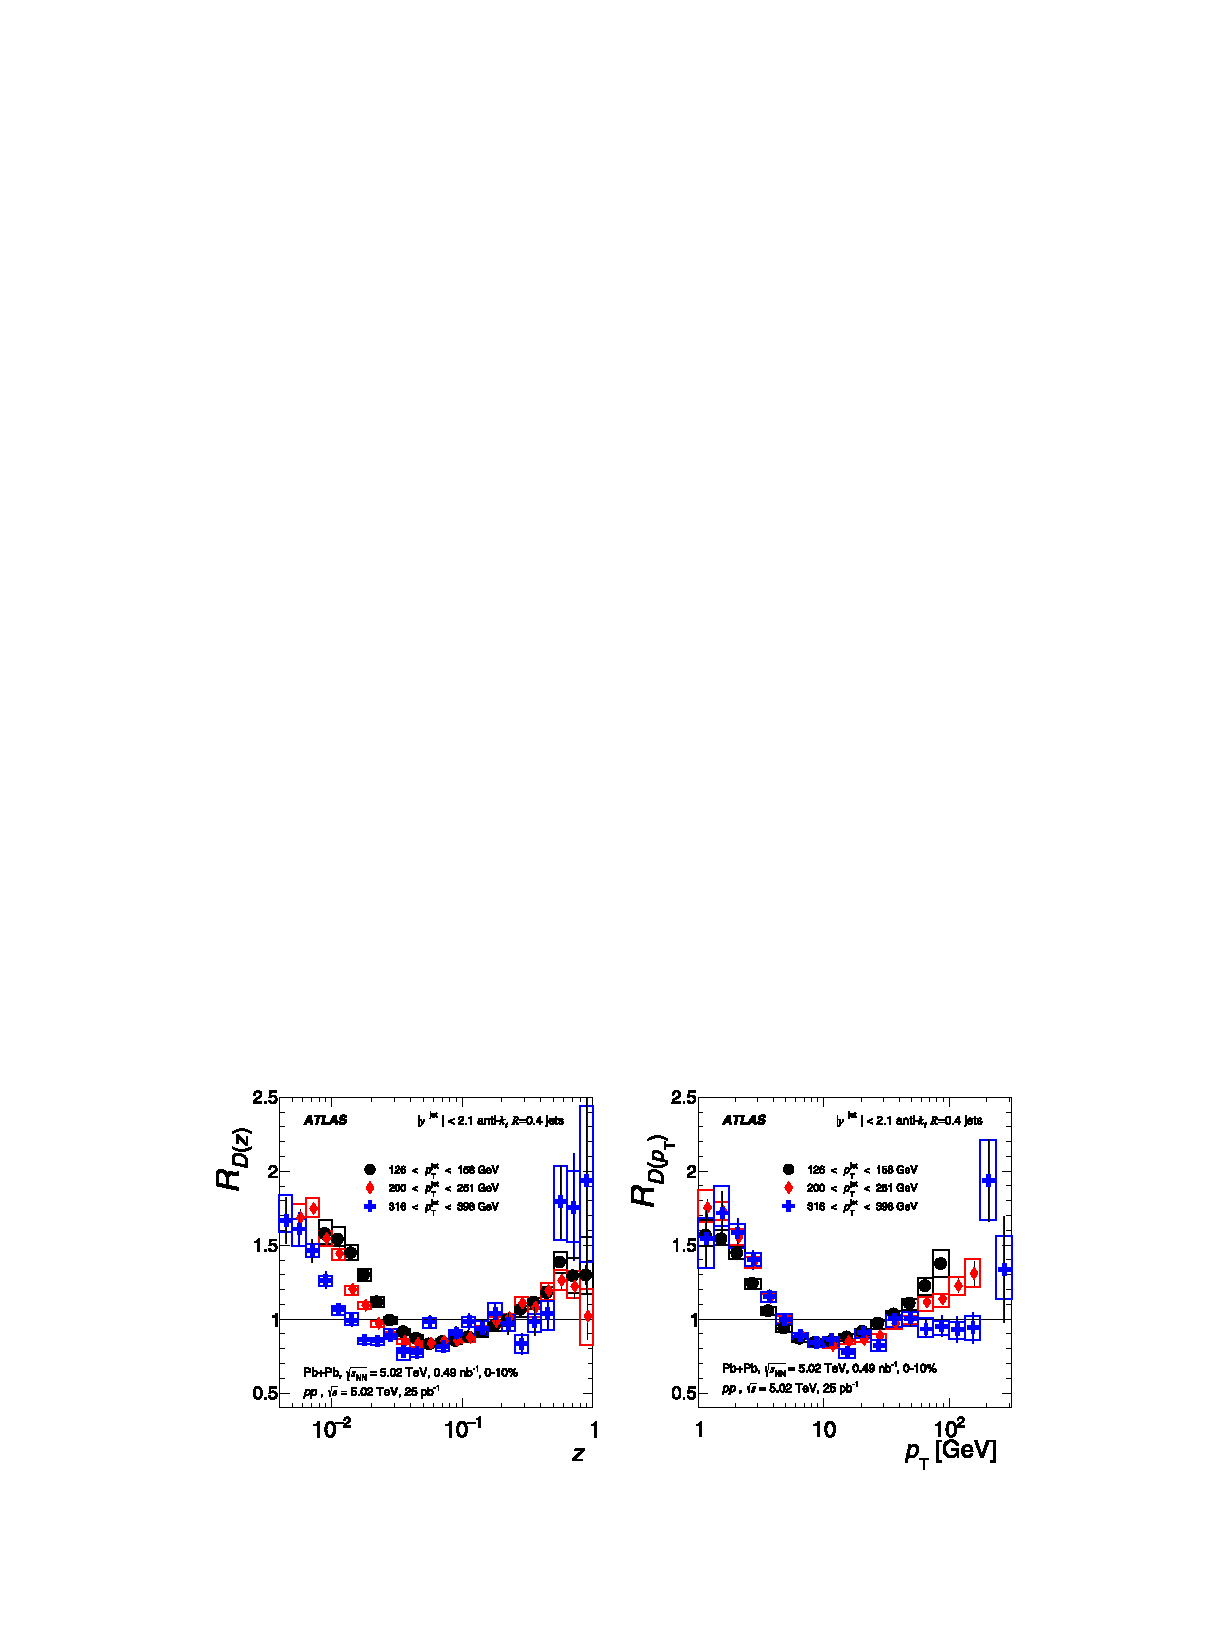
\includegraphics[width=0.75\textwidth]{figures/jetMeasurements/jetff_jetpt_dep}
\caption{The \ptjet\ dependence of the \Rdz\ (left) and \Rdpt\ (right) distributions in 0--10\% central \pbpb\ compared to \pp\ collisions. The error bars represent statistical uncertainties while the shaded boxes represent systematic uncertainties. Figure taken from \cite{PhysRevC.98.024908}.}
\label{fig:jetff_jetpt_dep}
\end{center}
\end{figure}


\begin{figure}[htbp]
\begin{center}
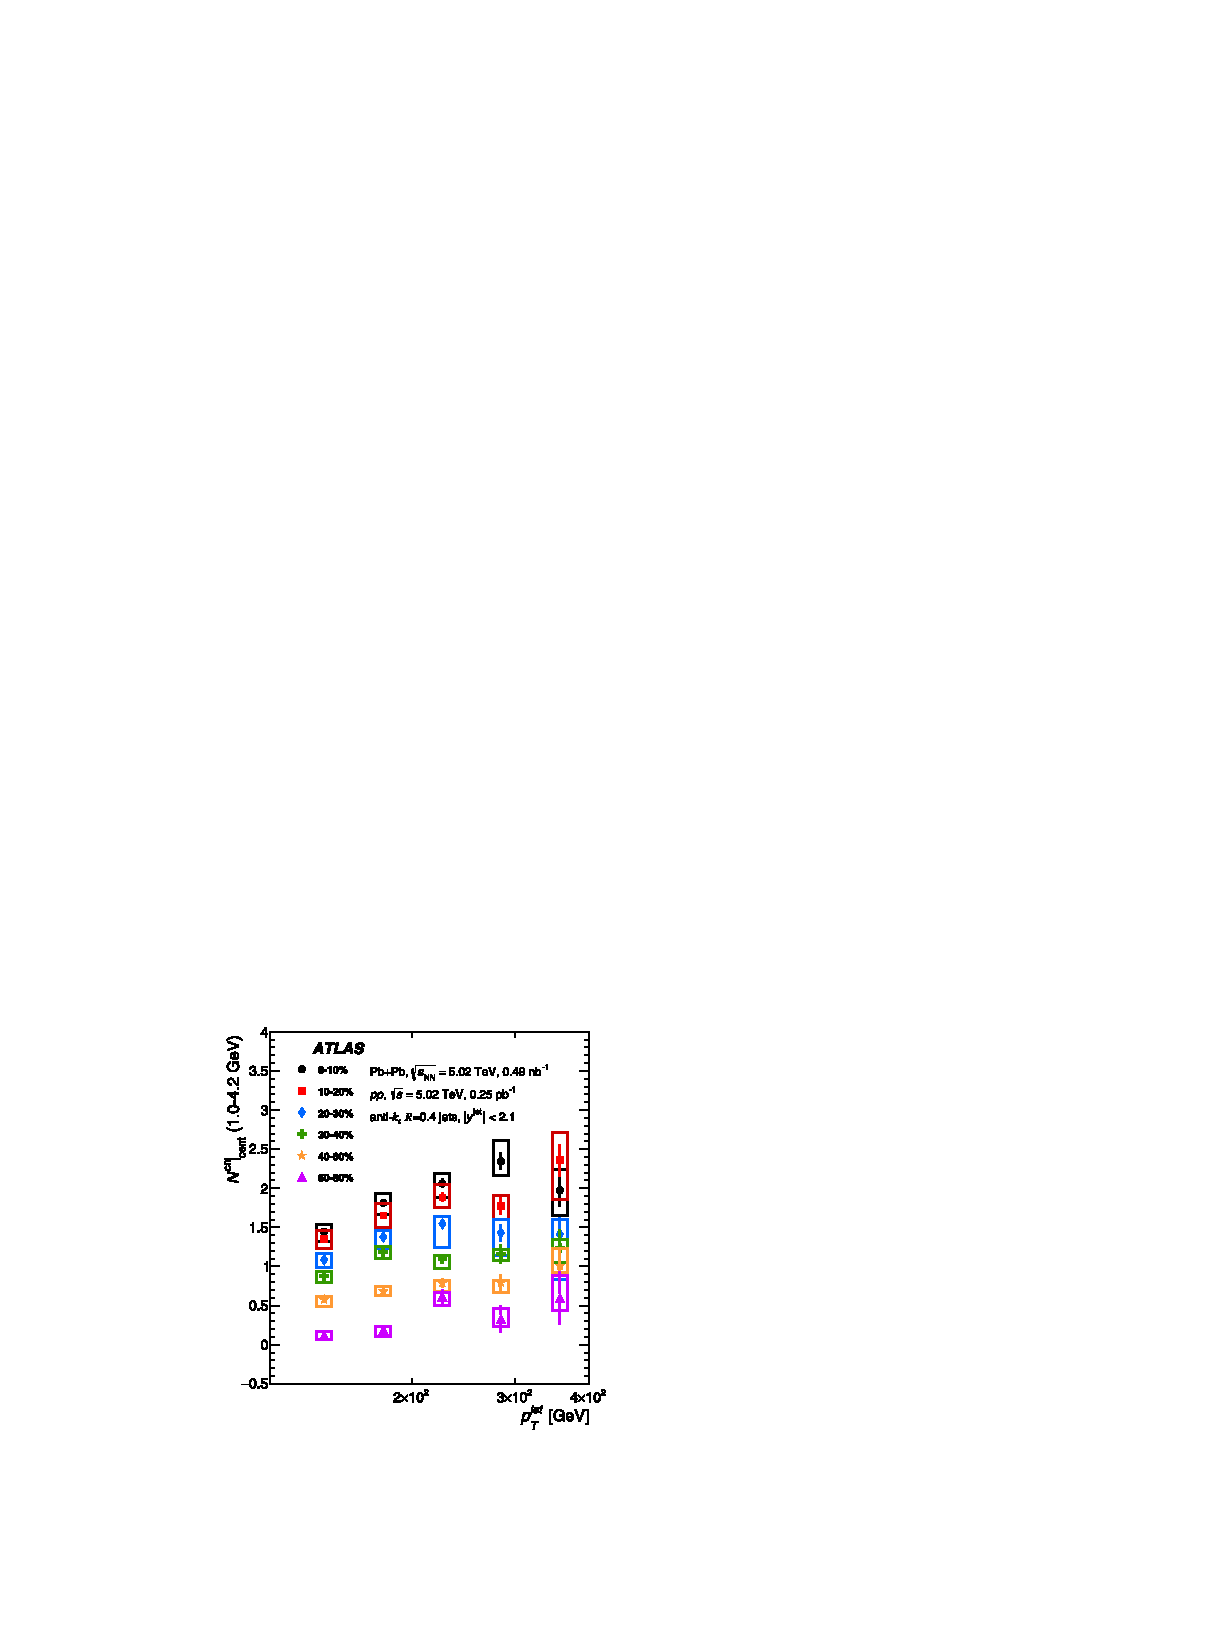
\includegraphics[width=0.35\textwidth]{figures/jetMeasurements/jetff_nch}
\caption{The number of extra particles that carry $1<\pt<4$ GeV  in \pbpb\ compared to \pp. The different colors represent different centrality selections. The error bars represent statistical uncertainties while the shaded boxes represent systematic uncertainties. Figure taken from \cite{PhysRevC.98.024908}.}
\label{fig:jetff_nch}
\end{center}
\end{figure}

The modifications to the \Dz\ distributions have also been compared to a variety of models, including the Effective Quenching model \cite{Spousta:2015fca}, the Soft Collinear Effective Theory \cite{Chien:2015vja, Kang:2017frl}, and the Hybrid Model \cite{Casalderrey-Solana:2014bpa}. These comparisons are shown in Figure~\ref{fig:jetff_rdz_theory}. It can be seen that 


\begin{figure}[htbp]
\begin{center}
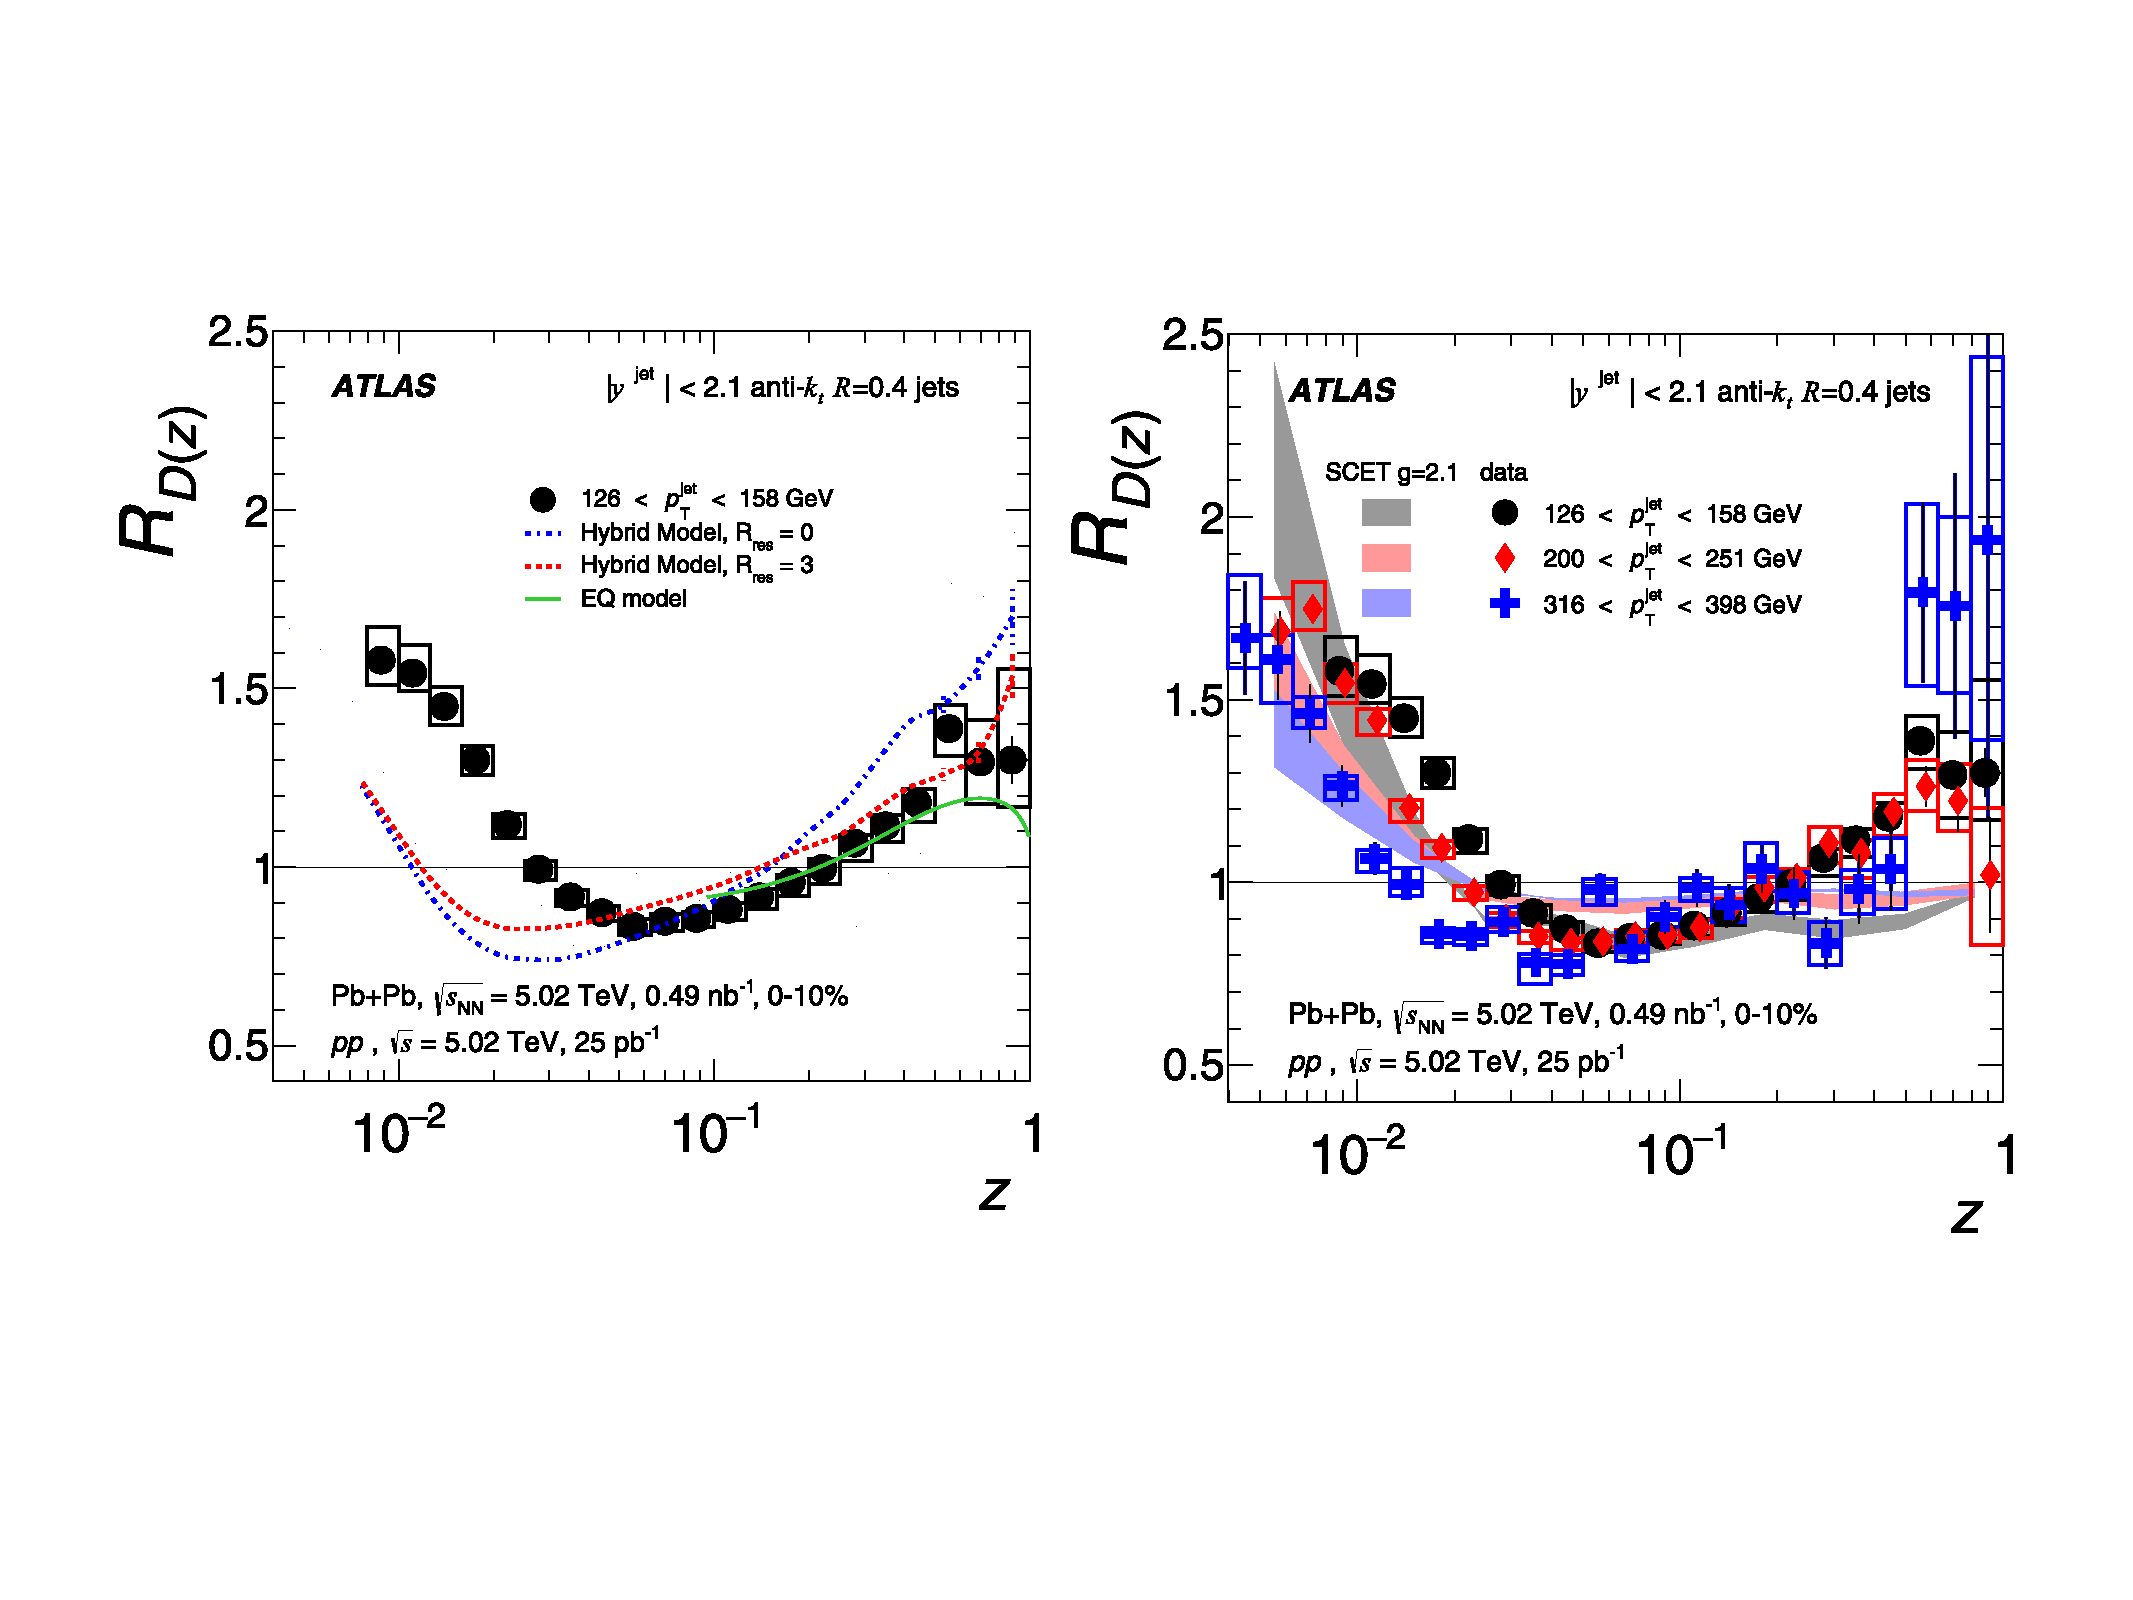
\includegraphics[width=0.75\textwidth]{figures/jetMeasurements/jetff_rdz_theory}
\caption{The \Rdz\ distributions compared to the EQ and Hybrid models (left) and SCET (right). The error bars represent statistical uncertainties while the shaded boxes represent systematic uncertainties. Figure taken from \cite{PhysRevC.98.024908}.}
\label{fig:jetff_rdz_theory}
\end{center}
\end{figure}



%%%%%%%%%%%%%%%%%%%%%%%%%%%%%%%%%%%%%%
\section{Effective Quenching}
This discussion is based on the model introduced in Ref. \cite{Spousta:2015fca}. This phenomenological model emphasizes the jet \pt\ dependence of the quark to gluon fraction and the difference between quark-jet and gluon-jet quenching. It uses an ``extended'' power law parameterization of the high-\pt\ hadron spectra coupled with a quenching that is based on a non-constant fractional energy loss. This model considers the different color charges carried by quarks and gluons and their different splitting functions, and assumes that gluon jets lose energy at a rate 9/4 times higher than quark jets. The key assumption of the model are:
\begin{itemize}
\item The energy lost by a jet is radiated at large angles and does not appear within the jet cone. This is backed by \cite{Chatrchyan:2011sx}.
\item The fragmentation pattern of the jet is unaffected by the presence of the QGP i.e. they fragment as they would in a vacuum. This is motivated by the idea that the QGP is unable to resolve the internal jet structure and is supported by \cite{Blaizot:2013hx, CasalderreySolana:2012ef}.
\end{itemize} 

The model uses the following extended power-law parameterization to describe the high-\pt\ jet spectra:

\begin{align}
\frac{dn}{d\ptjet} = A \left( \frac{\pt_0}{\ptjet} \right) ^{n+\beta \log(\ptjet / \pt_0)}
\end{align}

where $\pt_0$ is a reference transverse momentum at which $A= dn/d\ptjet$, $\beta$ is the logarithmic derivative of $dn/d\ptjet$ at $\ptjet = \pt_0$. Then considering the different quark and gluon fractions as $f_{q0}$ and $f_{g0} = 1-f_{q0}$ respectively, the combined spectrum for quarks and gluons can be written as:

\begin{align}
 \frac{dN}{d\ptjet} &= A \left[ f_{q0} \left( \frac{\pt_0}{\ptjet} \right)^{n_q+ \beta_q \log(\ptjet / \pt_0)} + (1-f_{q0}) \left( \frac{\pt_0}{\ptjet} \right)^{n_g + \beta_g \log(\ptjet / \pt_0)} \right] \\
\nonumber \\ 
\label{eq:eq_q_frac} f_q (\ptjet) &= \dfrac{1}{1 + \left(\dfrac{1-f_{q0}}{f_{q0}}\right) \left( \dfrac{\pt_0}{\ptjet}\right)^{\Delta n + \Delta \beta \log(\ptjet/\pt_0)} }
\end{align}
where $\Delta n = n_g - n_q$ and $\Delta \beta = \beta_g - \beta_q$. The \pt\ dependence of the quark fraction along with the fit is shown in Figure~\ref{fig:raa_centDep}. The fragmentation functions can also be determined using final-state charged hadrons within a $R=0.4$ jet cone. These are fit to the form \Dz, with fits for the quark and gluon fragmentation shown in Figure~\ref{fig:gluon_fragmentation}.


\begin{align}
D(z) = a \times \frac{(1+dz)^b}{(1+ez)^c} \times e^{-fz}
\label{eq:ff_param}
\end{align}


\begin{figure}
\begin{subfigure}{.45\textwidth}
  \centering
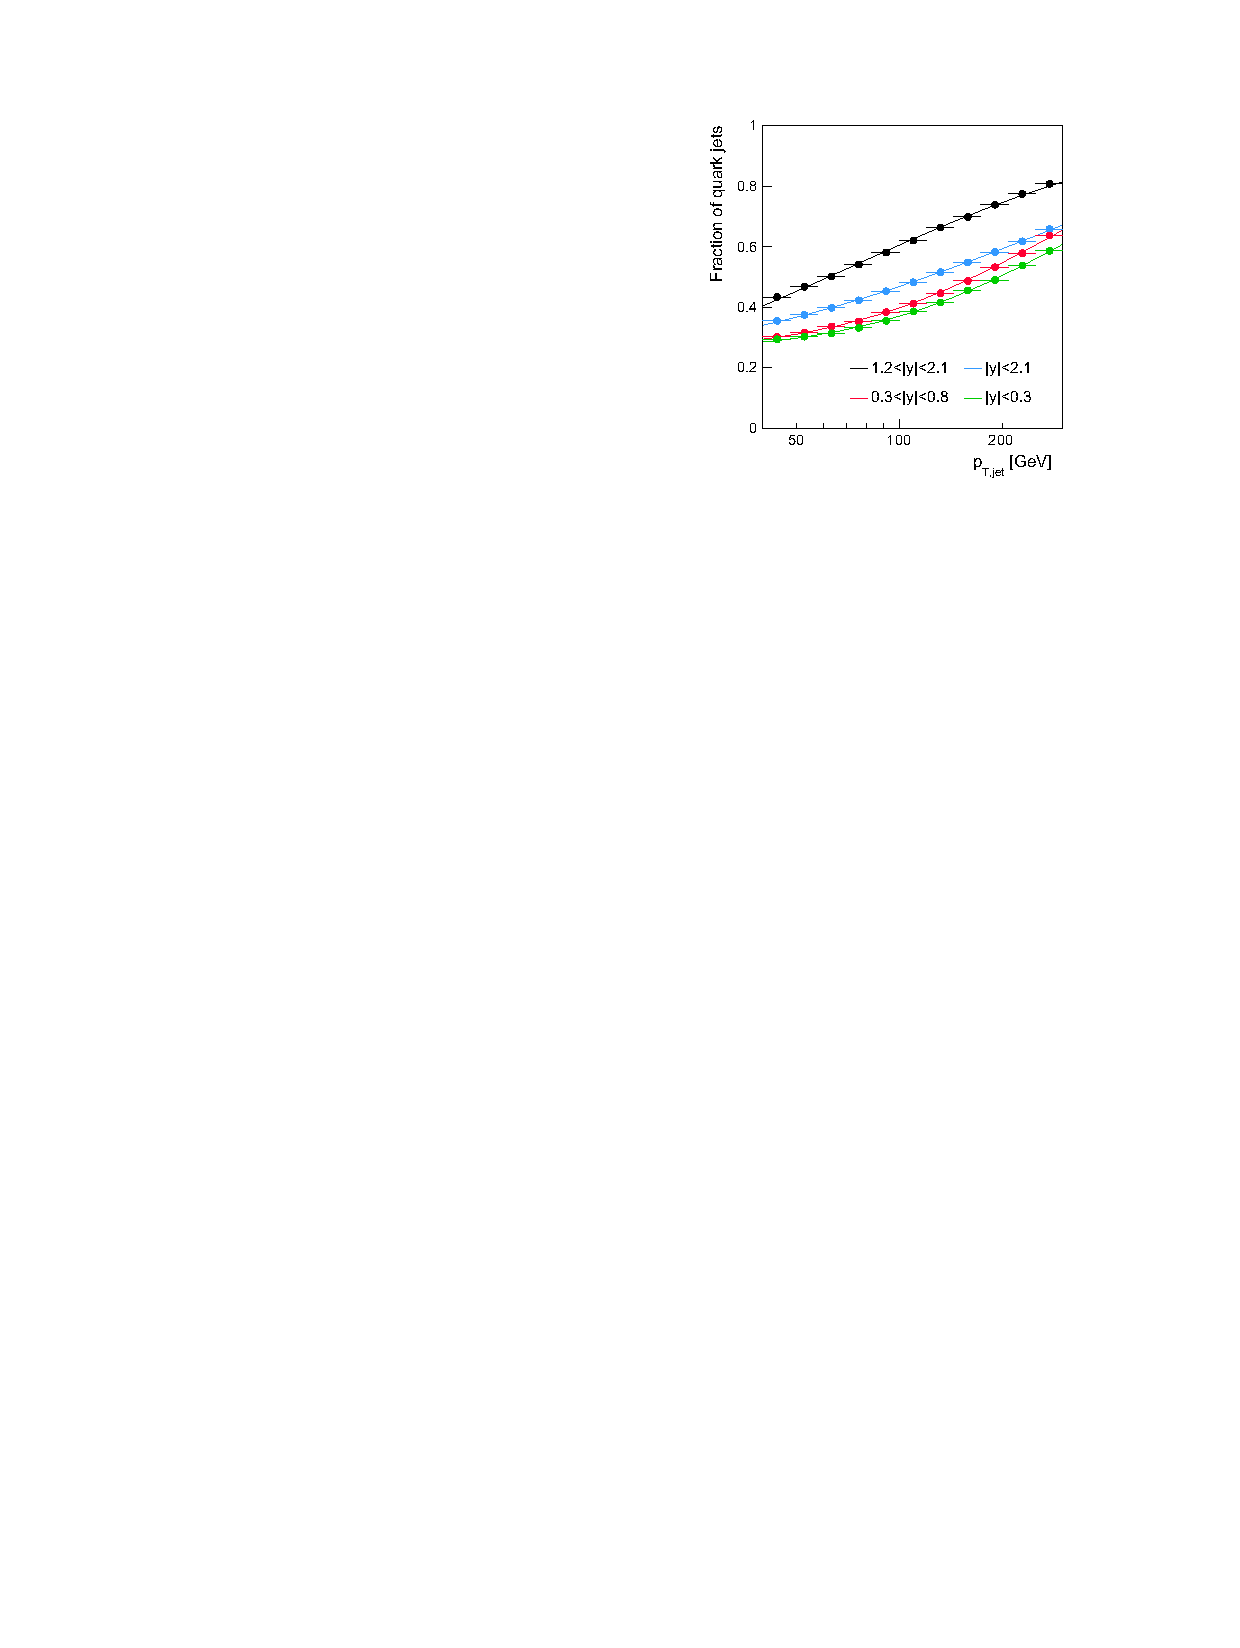
\includegraphics[width=0.8\textwidth]{figures/jetMeasurements/jetQuarkFraction}
\caption{The jet quark fraction as a function of \ptjet\ in different rapidity bins. The points are from \pythia8 simulations and the lines are fits to Equation~\ref{eq:eq_q_frac}.}
\label{fig:raa_centDep}
\end{subfigure} \qquad
\begin{subfigure}{.45\textwidth}
  \centering
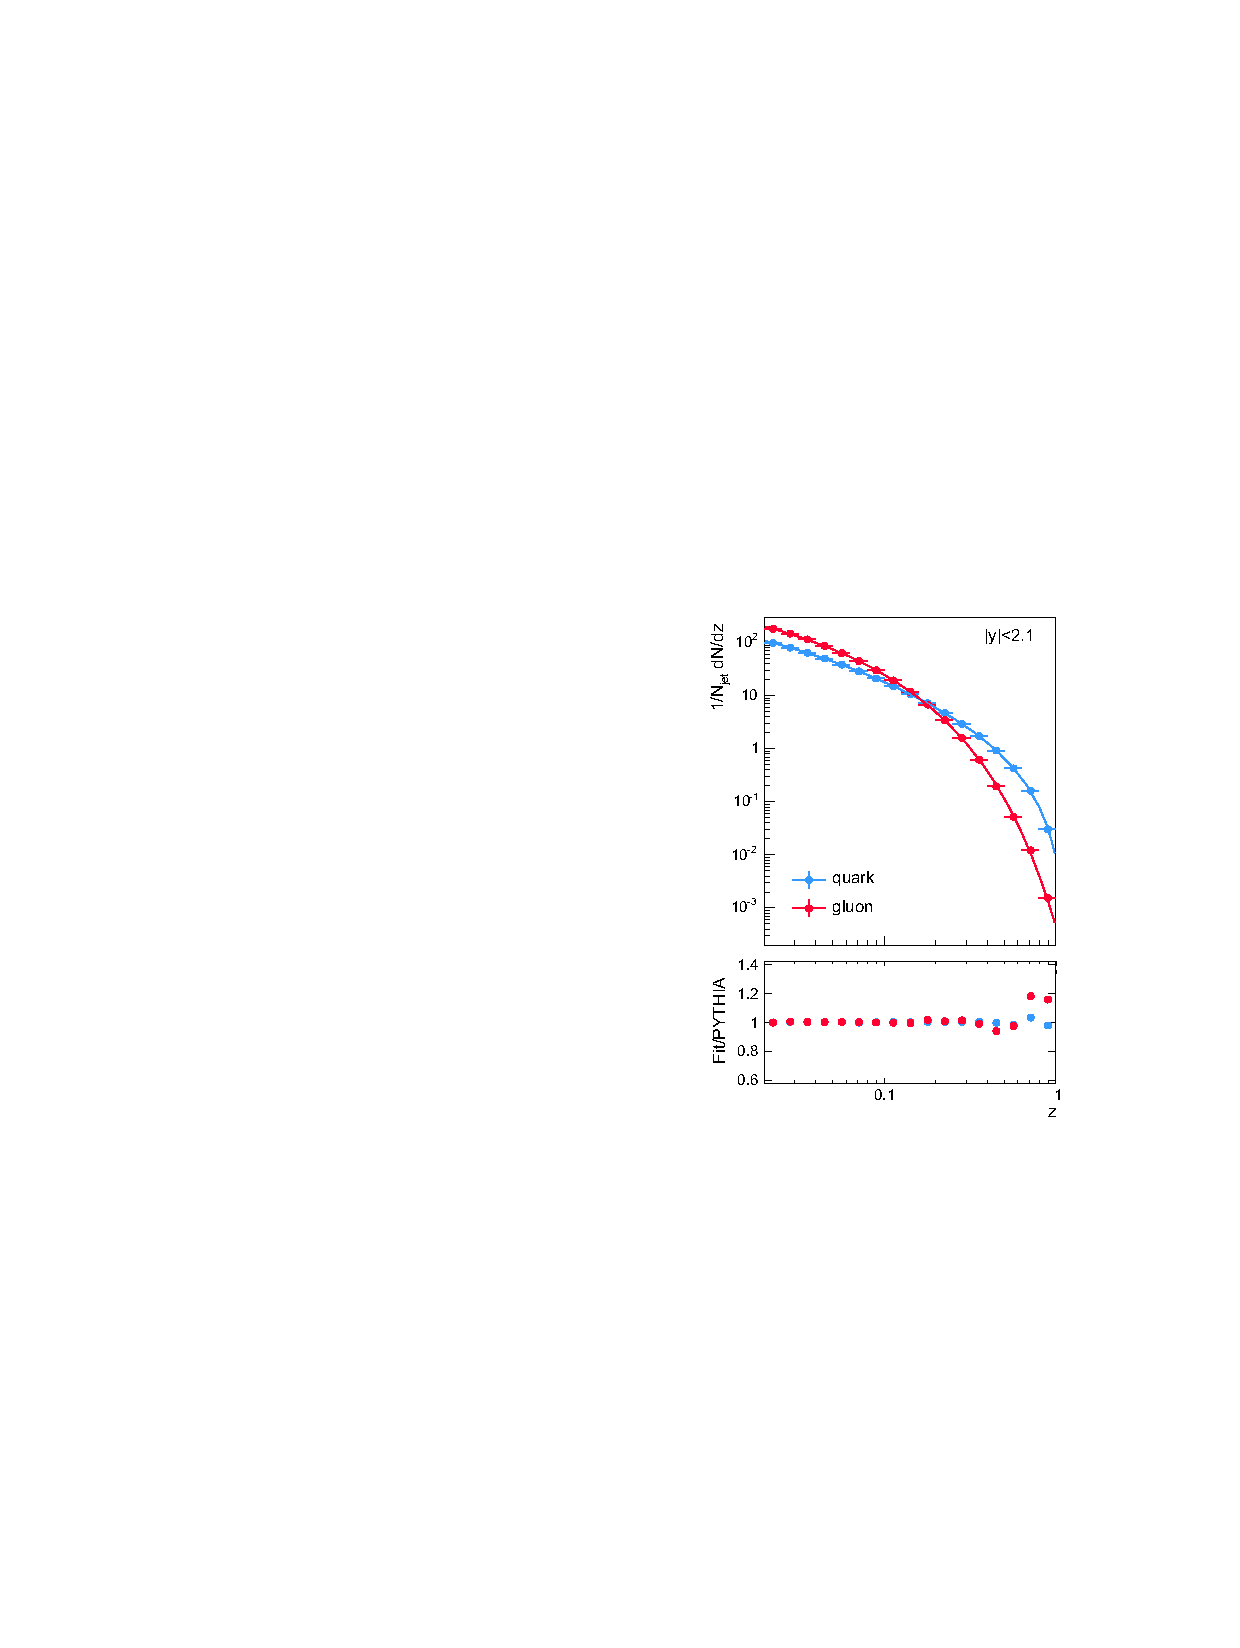
\includegraphics[width=0.8\textwidth]{figures/jetMeasurements/gluon_fragmentation}
\caption{A comparison of the \pythia8 quark and gluon fragmentation. The solid lines are the fits from The jet quark fraction as a function of \ptjet\ in different rapidity bins. The points are from \pythia8 simulations and the lines are fits to Equation~\ref{eq:ff_param}.}
\label{fig:gluon_fragmentation}
\end{subfigure}
\caption{Fits to quark fractions and fragmentation functions from \pythia8.  Figure taken from \cite{Spousta:2015fca}}
\label{fig:EQ_pp_models}
\end{figure}


For the quenched spectra, this model assumes a non-constant fractional shift given below as $S$. This approach is based on \cite{baier2001quenching} and is used because of the inability of the constant fractional shift to explain the jet \pt\ dependence of measured \RAA. 

\begin{align}
S = s' \left( \frac{\ptjet}{\pt_0} \right) ^\alpha
\end{align}
where $\alpha$ is an undetermined parameter and $s'$ is the shift for a jet with $\ptjet = \pt_0$. This gives the following quenched high-\pt\ hadron spectra:

\begin{align}
 \frac{dN_Q}{d\ptjet} &= A \Bigg[ f_{q0} \left( \frac{\pt_0}{\ptjet+S_q} \right)^{n_q+ \beta_q \log\big((\ptjet+S_q) / \pt_0\big)} \left(1 + \frac{dS_q}{d\ptjet} \right) \\
& + (1-f_{q0}) \left( \frac{\pt_0}{\ptjet+S_g} \right)^{n_g + \beta_g \log\big((\ptjet+S_g) / \pt_0\big)}  \left(1 + \frac{dS_g}{d\ptjet} \right) \Bigg] \nonumber
\end{align}
Where the $(1+dS/d\ptjet)$ term is a Jacobian to preserve the number of jets. 
Then the \RAA\ can be written as:

\begin{align}
\RAA = f_q & \left(\frac{1}{1 + S_q / \ptjet}\right) ^{n_q + \beta_q \log\big((\ptjet+S_q)/\pt_0\big)}  \frac{\pt_0}{\ptjet}^{} \left( 1+ \frac{dS_q}{d\ptjet} \right) \times  \\
 (1-f_q) & \left(\frac{1}{1 + S_g / \ptjet}\right) ^{n_g + \beta_g \log\big((\ptjet+S_g)/\pt_0\big)}  \frac{\pt_0}{\ptjet}^{} \left( 1+ \frac{dS_g}{d\ptjet} \right)  \nonumber \\
\end{align}
where the flavor fraction is given by Equation~\ref{eq:eq_q_frac}. These can be fit to the measured ATLAS \RAA\ data as shown in Figure~\ref{fig:EQ_RAA} and the parameters $s'$ and $\alpha$ can be extracted as shown in Figure~\ref{fig:eq_param}. 

\begin{figure}[htbp]
\begin{center}
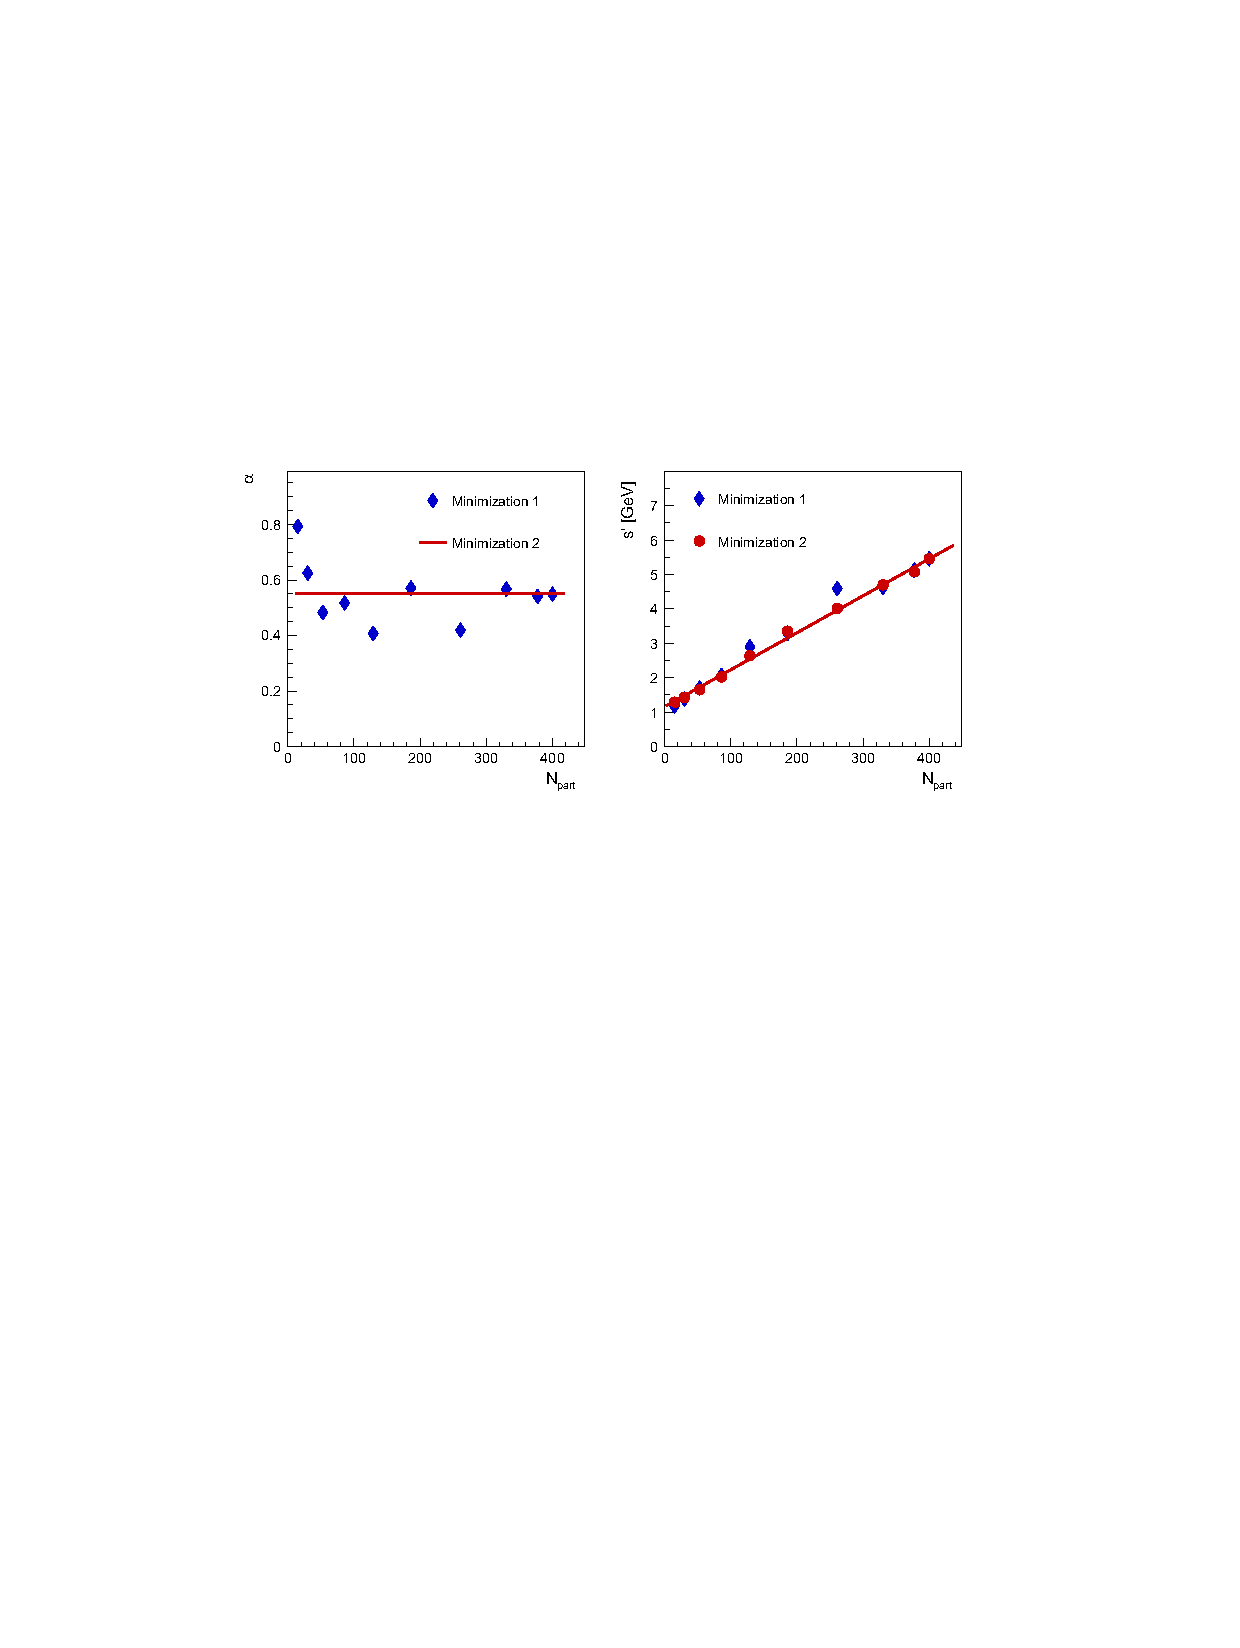
\includegraphics[width=0.55\textwidth]{figures/jetMeasurements/EQ_fitQuality}
\caption{The extracted values of $\alpha$ and $s'$ as a function of \Npart. The first minimization shows fluctuations for $\alpha$ around 0.55, which was then fixed for the second minimization to give an $s'$ that linearly depends on \Npart. Figure taken from \cite{Spousta:2015fca}}
\label{fig:eq_param}
\end{center}
\end{figure}

It can be seen that the analytic fits and the MC are in good agreement. While the fits agree with the data by definition, the robustness of the model can be seen in that it describes the data with a single value for $\alpha$ and a simple centrality dependent shift constant $s'$.  Fits to the \Dz\ distributions are shown in Figure~\ref{fig:EQ_FF} and it can be seen that while the MC and analytic calculation agree well with each other, they are only able to qualitatively capture some features of the data. The enhancement at high $z$ can be explained by an increased quark content of the jet spectrum and subsequent differential quenching for quark and gluon jets. The low $z$ enhancement on the other hand can be considered to be a result of a gluon radiation within the jet or a wake from the medium itself.

\begin{figure}
\begin{subfigure}{1\textwidth}
  \centering
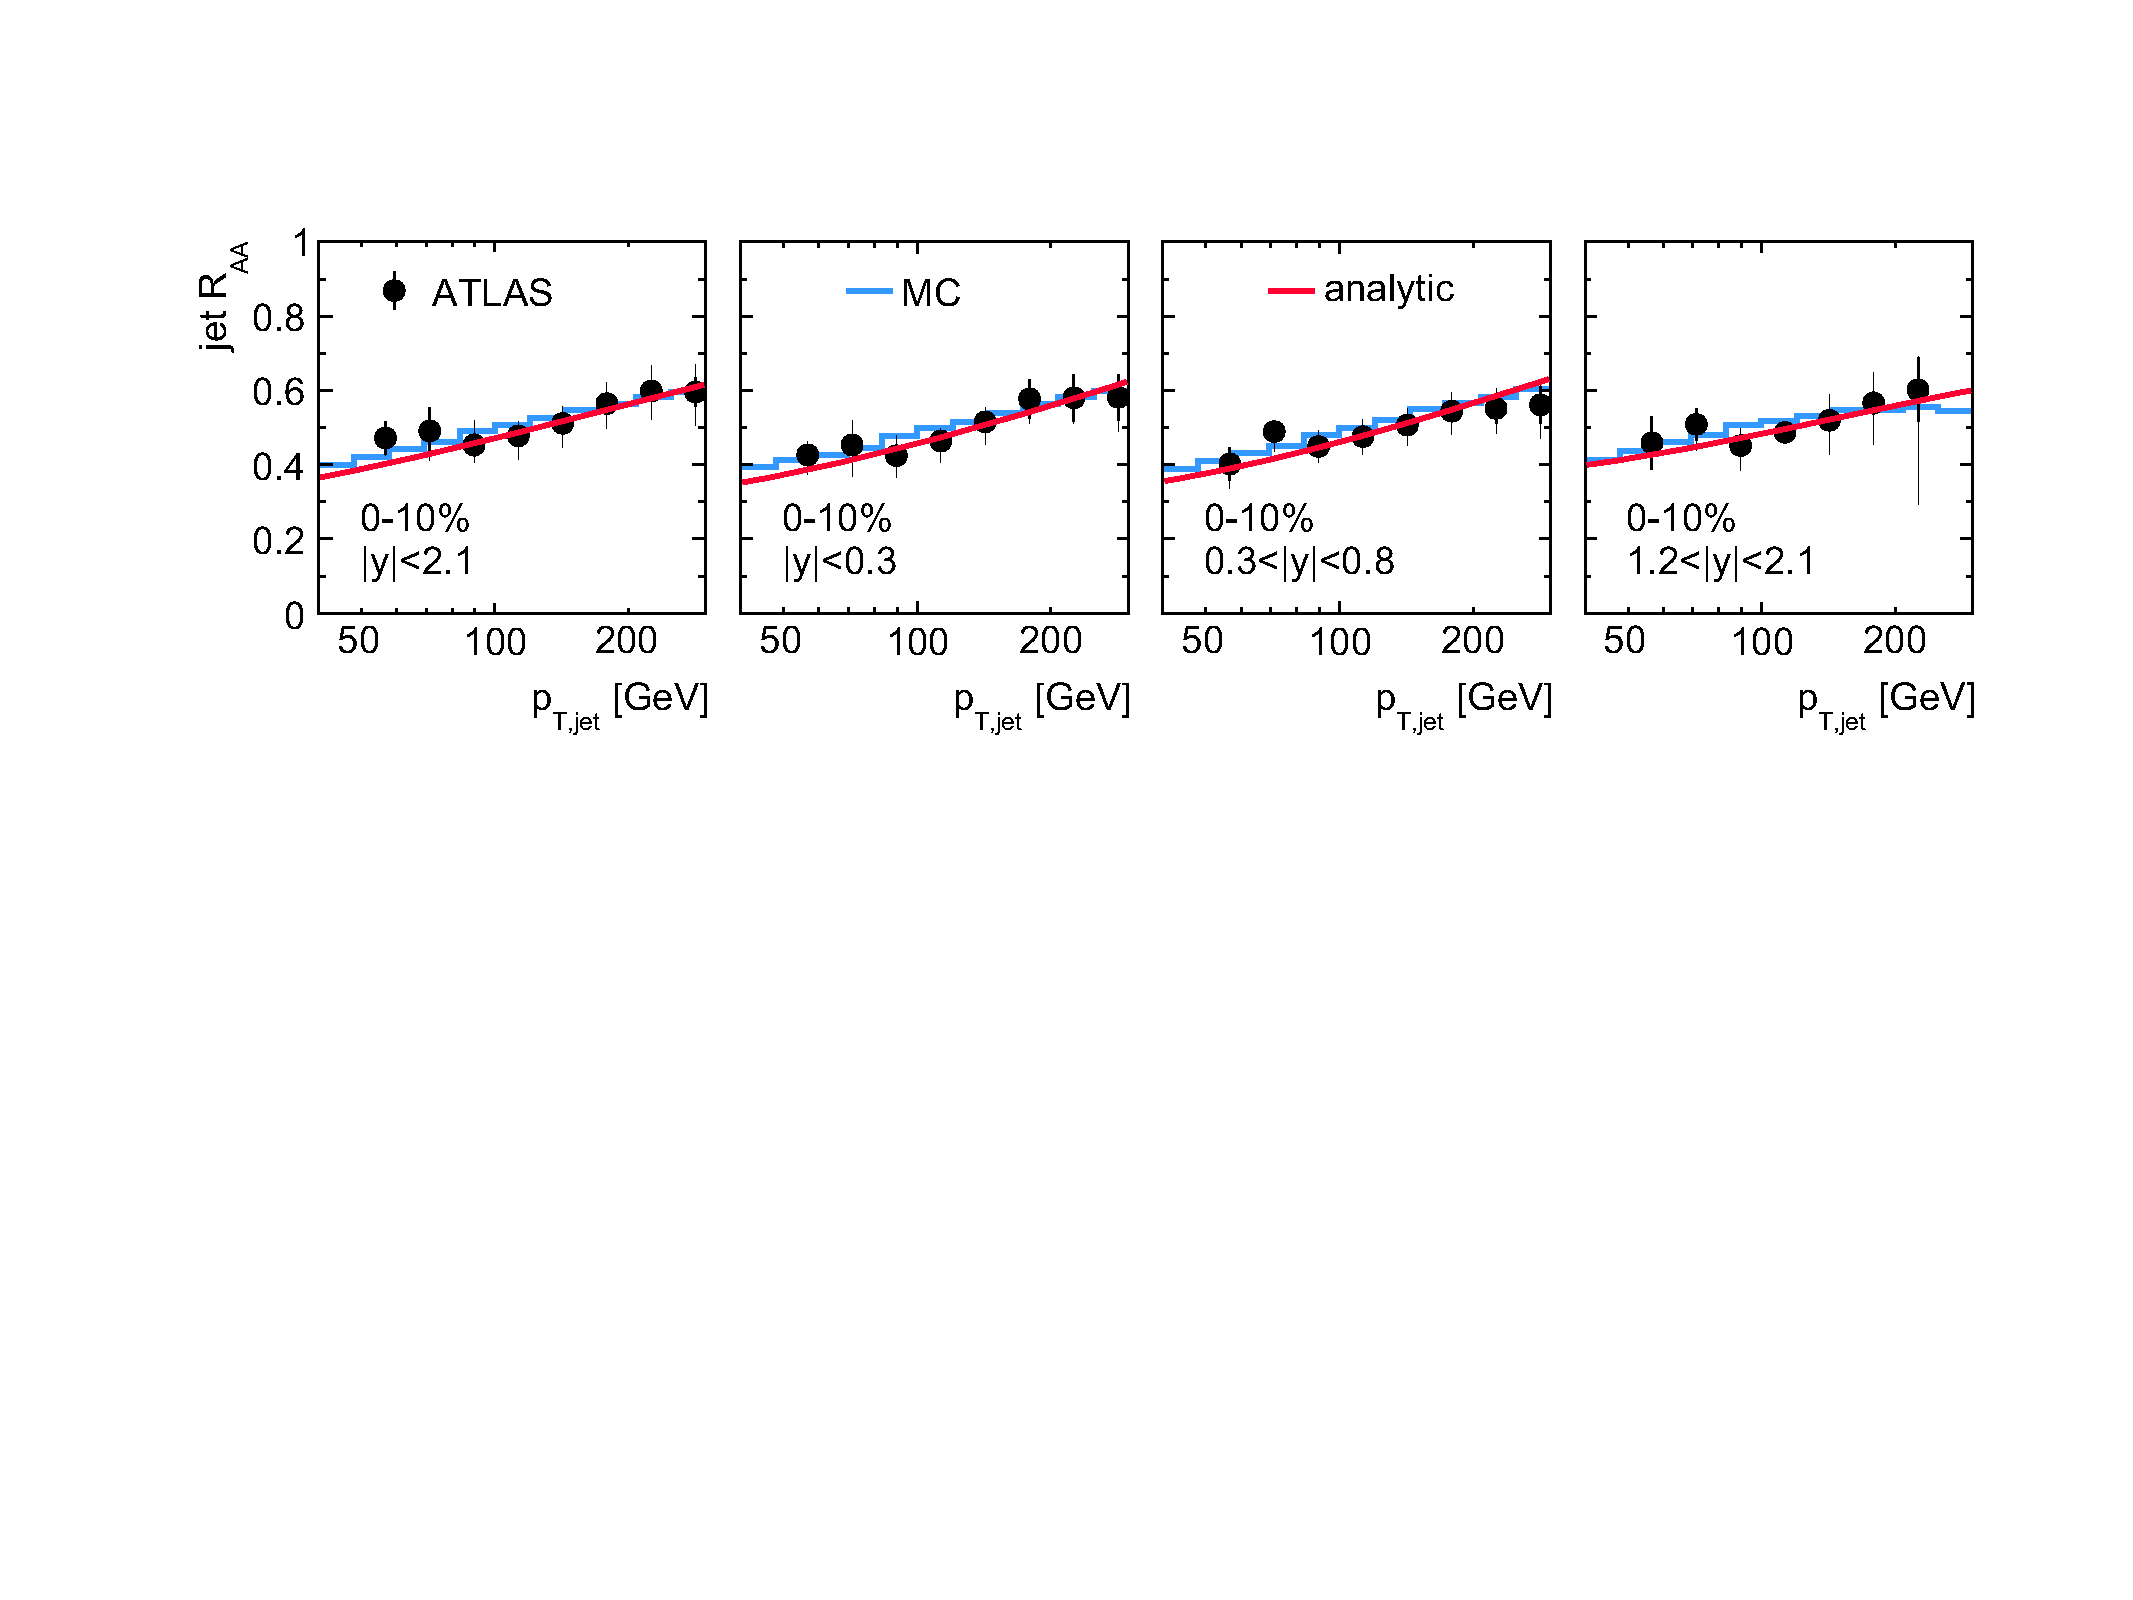
\includegraphics[width=1\textwidth]{figures/jetMeasurements/EQ_RAA}
\caption{A comparison of the \RAA\ as measured by ATLAS for central \pbpb\ collisions in \cite{Aad:2014bxa}, a MC calculation (blue) and the analytic calculation (red) in the EQ model with the extended power-law parameterization and a non-constant fractional energy loss. The different panels are different rapidity intervals.}
\label{fig:EQ_RAA}
\end{subfigure} \\ \\ \\
\begin{subfigure}{1\textwidth}
  \centering
\includegraphics[width=1\textwidth]{figures/jetMeasurements/eq_FF}
\caption{A comparison of the \Rdz\ as measured by ATLAS in \cite{Aad:2014wha}, a MC calculation (blue) and the analytic calculation (red) in the EQ model with the extended power-law parameterization and a non-constant fractional energy loss. The different panels are different centrality intervals.}
\label{fig:EQ_FF}
\end{subfigure}
\caption{A comparison of measured data, MC, and the analytic calculation of the EQ model. Figure taken from \cite{Spousta:2015fca}}
\label{fig:EQ_modification}
\end{figure}




%%%%%%%%%%%%%%%%%%%%%%%%%%%%%%%%%%%%%%
\section{Jet Fluid model}
This discussion is based on the model introduced in Ref. \cite{Tachibana:2017syd}. This model considers the evolution of the jet and QGP in a coupled manner, considering the energy and transverse momentum exchange between them. In this picture, both the jet and medium are allowed to modify each other; the jet is modified via collisional and radiative processes while the medium evolves hydrodynamically and is modified because it picks up the energy lost by the jet. 

The time evolution of the jet is given 

\begin{align}
f_i (\omega_i, \kTsq_i, t) = \frac{dN_i (\omega_i \kTsq_i, t)}{d \omega_i d\kTsq_i}
\end{align}
where $i$ is the type of parton, $\omega_i$ is its energy, and $\kTsq$ is its transverse momentum with respect to the jet axis. Then the transport equations can be written in terms of :

\begin{align}
\label{eq:jf_transportEq}
\frac{d f_j}{dt} &= \hat{e_j} \frac{\p f_j}{\p \omega_j} + \frac{1}{4} \hat{q_j} \nabla_{\kT}^2 f_j  \\
& + \sum_i \int d\omega_i d\kTsq_i \frac{d\widetilde{\Gamma}_{i\rightarrow j} }{d\omega_j d\kTsq_j dt} f_i \\
& - \sum_i \int d\omega_i d\kTsq_i \frac{d\widetilde{\Gamma}_{j\rightarrow i} }{d\omega_ij d\kTsq_i dt} f_i \\
\end{align}
where the first term is the collisional energy loss, the second term is the transverse momentum broadening, and the last two terms are the medium induced gain and loss radiative processes respectively. The splitting processes are are given by:

\begin{align}
\frac{d\Gamma_{i \rightarrow j}}{d \omega_j d\kTsq_j dt} = \frac{2\alpha_S}{\pi} \hat{q}_g \frac{x P_{i \rightarrow j} (x)}{\omega_j {k_{\rm T}^4}_j} \sin^2 \left(\dfrac{t - t_i}{2\tau_f} \right)
\end{align}
where $P_{i \rightarrow j} $ is the vacuum splitting function for $i \rightarrow j $ with $\omega_j$ being the energy of the radiated parton, $\tau_f$ is the formation time of the radiated parton, and $\kT_j$ is the transverse momentum of the radiated parton with respect to the parent parton. These transport Equations~\ref{eq:jf_transportEq} can be solved numerically and agree with \RAA\ measurements \cite{Aad:2014bxa, Khachatryan:2016jfl, Abelev:2013kqa}. The effects of the medium are included by considering the energy-momentum conservation of the jet-QGP system $ \p_\mu [T_{\rm QGP}^{\mu\nu} + T_{\rm jet}^{\mu\nu}] = 0$. Then the source term $J^\nu(x)$ that describes the energy transfer between the jet and the medium can be defined as $J^\nu(x) \equiv -\p_\mu  T_{\rm jet}^{\mu\nu}$, making the QGP evolution being given by

\begin{align}
 \p_\mu T_{\rm QGP}^{\mu\nu} = j^\nu
\end{align}
which characterizes the energy-momentum transfer between the jet and the QGP. 

An important component of this model is the flow induced by jets. A snapshot of this is shown in Figure~\ref{fig:jf_snapshot}, where the evolution of the energy density of the medium can be seen in a sample event. A single jet travels through the QGP, and can be clearly seen in the lower panels after the energy of the medium has been subtracted out. The V shaped feature seen is the mach cone that is induced by the parton as it moves faster than the medium sound velocity. 

\begin{figure}[htbp]
\begin{center}
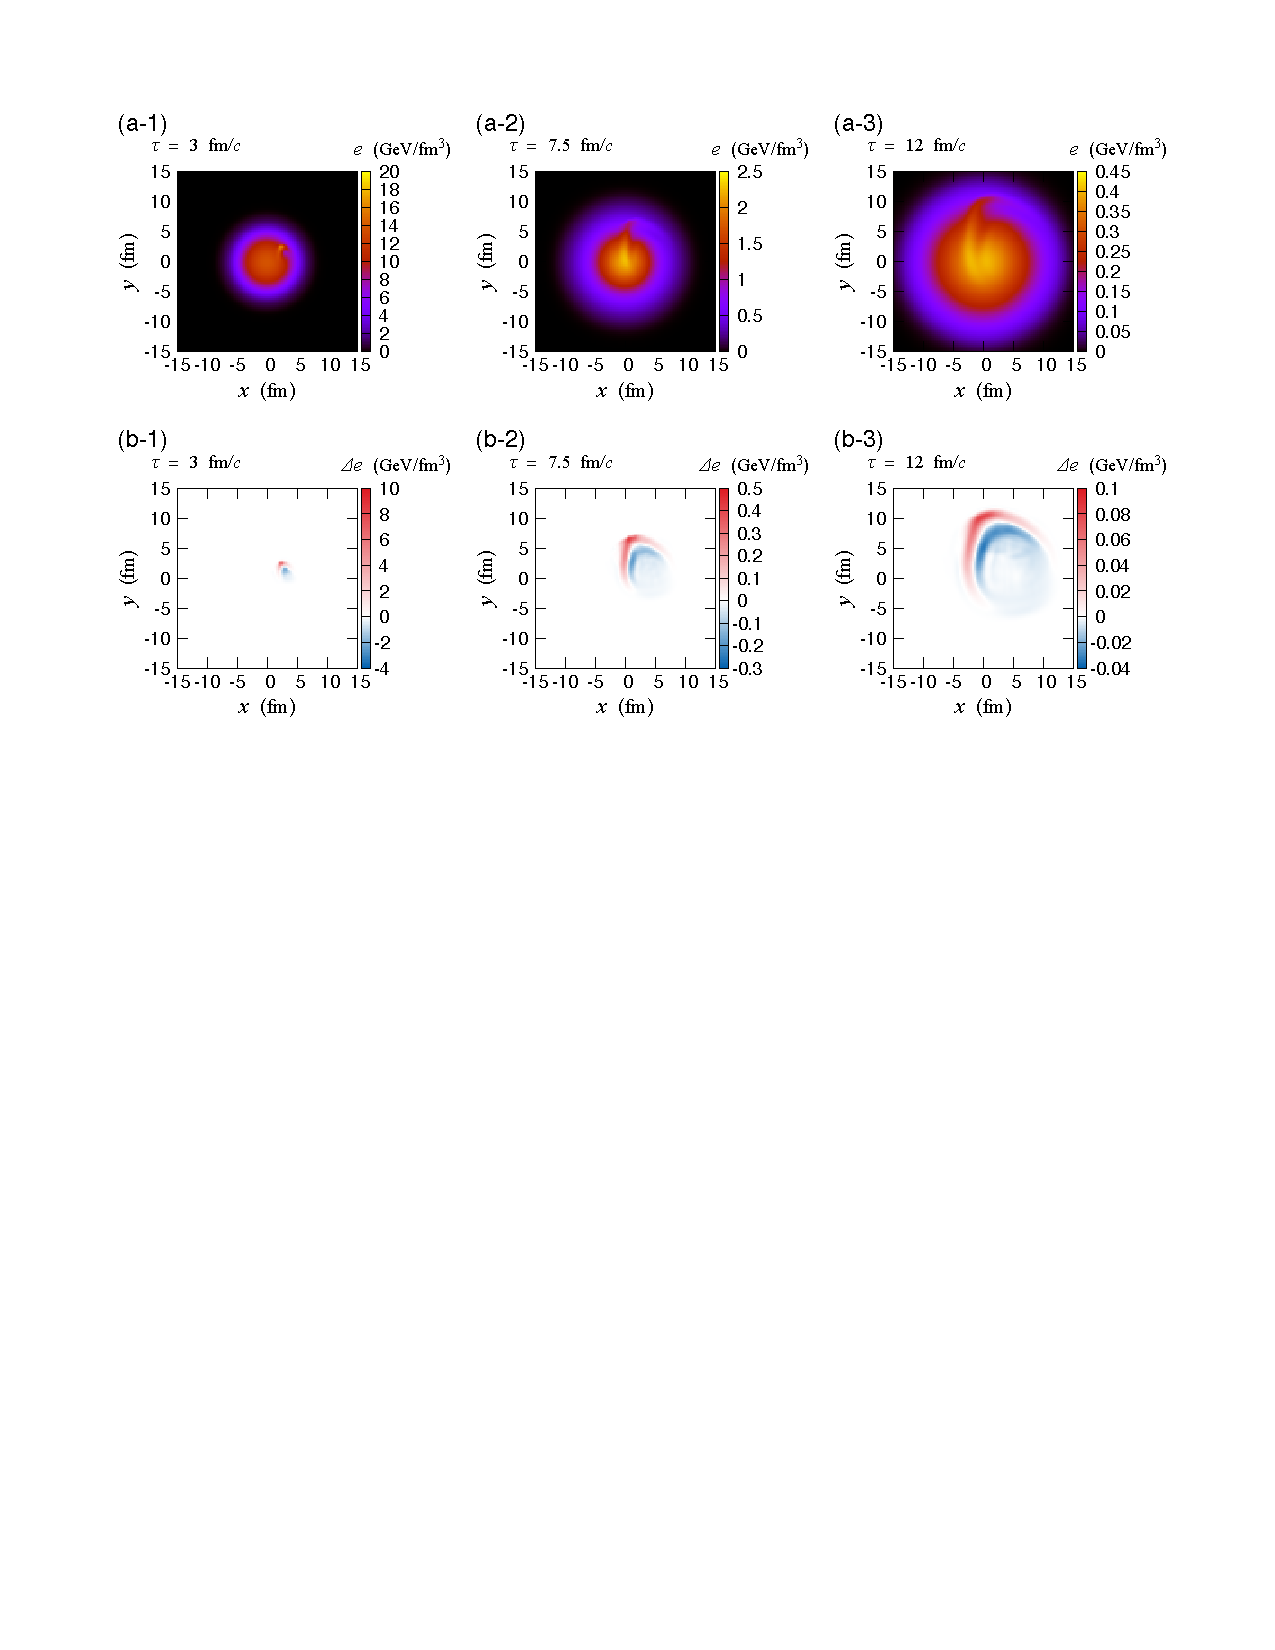
\includegraphics[width=0.85\textwidth]{figures/jetMeasurements/JF_snapshot}
\caption{(Top) The time evolution of the energy density of the quark gluon plasma with a jet propagating through it. (Bottom) The time evolution of the energy density in the event after the energy density of the QGP has been subtracted out. Figure taken from \cite{Tachibana:2017syd}.}
\label{fig:jf_snapshot}
\end{center}
\end{figure}

The final jet energy has two components: the jet shower, and the hydrodynamic response. The former as discussed above comprises of the collisional energy loss, momentum broadening, and medium induced radiation. The latter includes the energy lost from the jet shower that thermalizes into the medium and induces conical flow, some of which is still in the jet cone. This compensates some of the energy lost in the shower and can be seen in Figure~\ref{fig:jf_energyLoss}. While the absolute amount of energy lost increases as a function of initial jet energy, the fractional energy loss decreases. Furthermore there is a cone size dependence once the hydrodynamic contributions are included. This is a result of the jet being highly collimated, such that while an increase in the size does not change the energy much, it does affect the hydrodynamic contribution from the medium.
\begin{figure}[htbp]
\begin{center}
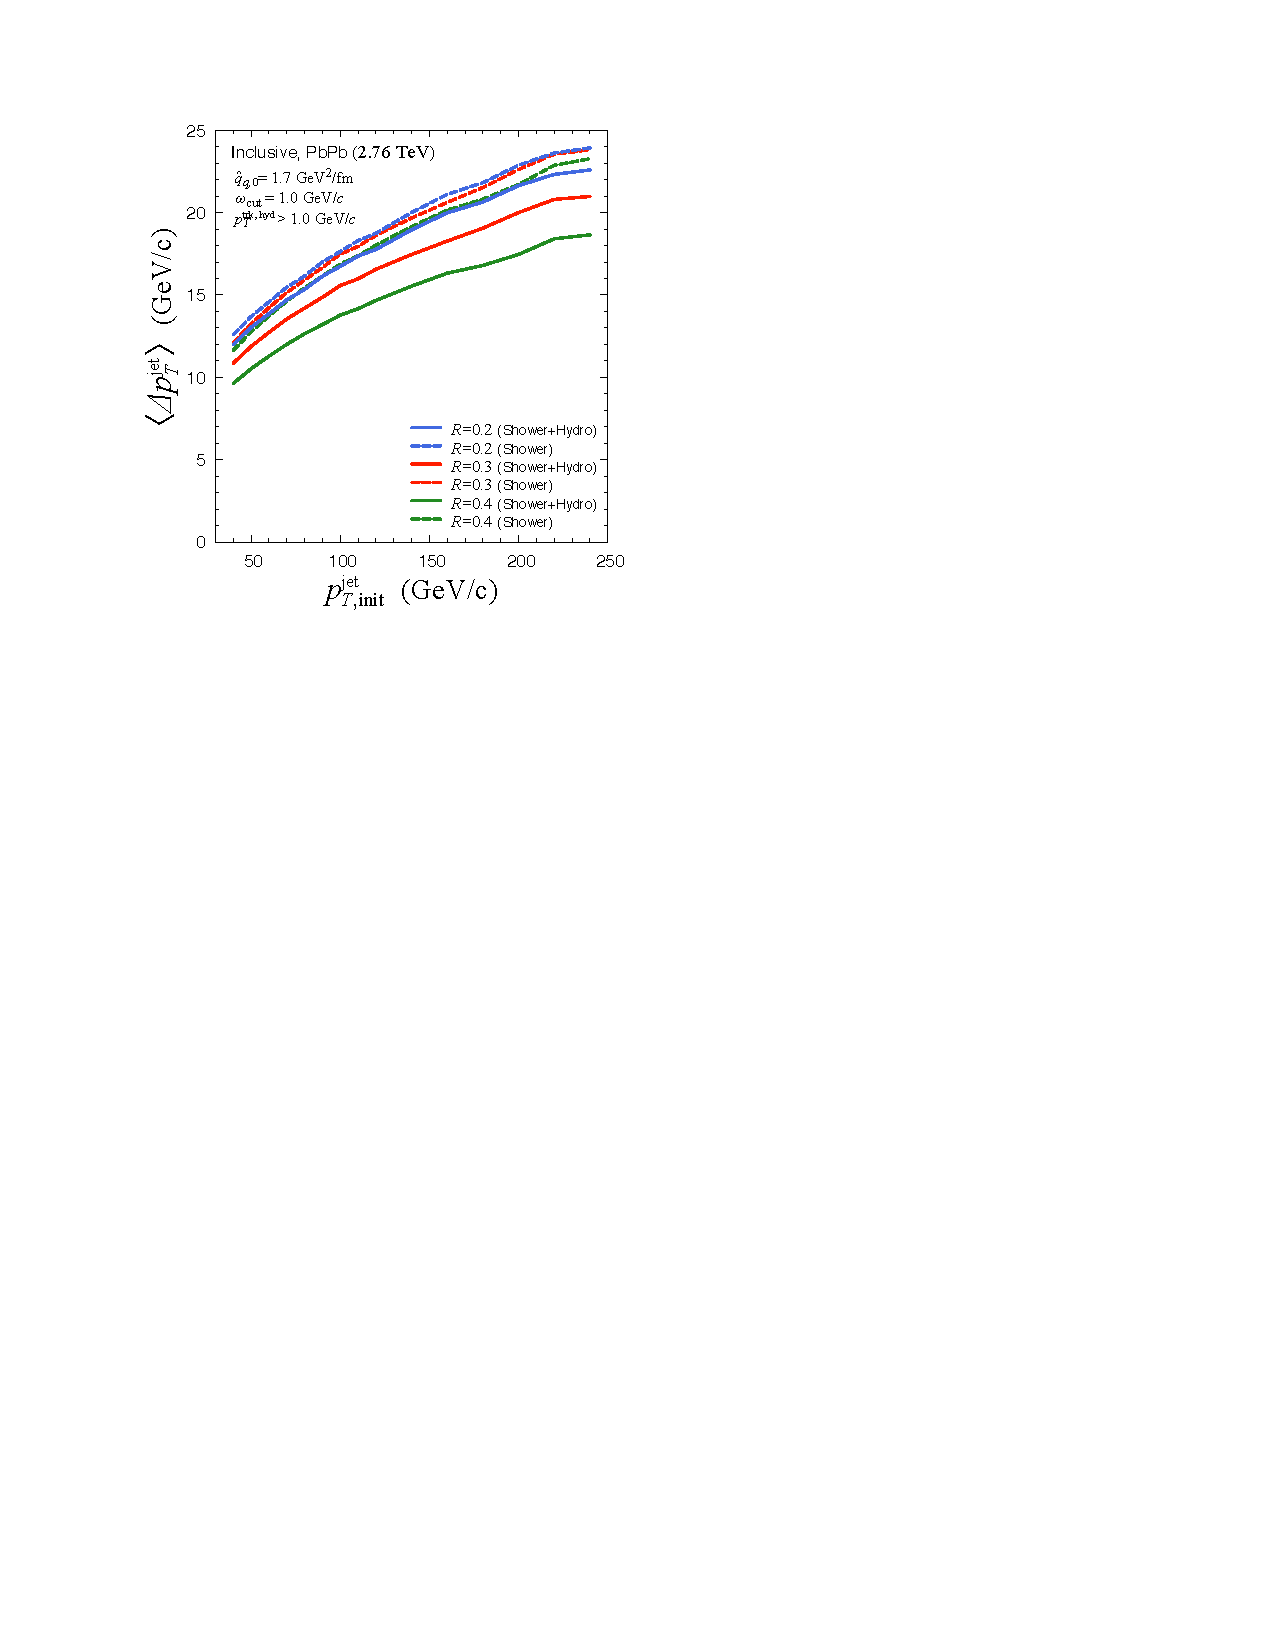
\includegraphics[width=0.45\textwidth]{figures/jetMeasurements/JF_energyLoss}
\caption{(Top) The energy lost by a jets of different radii as a function of their initial energy in central \pbpb\ collisions at \sqrtsnn = 2.76 TeV. Figure taken from \cite{Tachibana:2017syd}.}
\label{fig:jf_energyLoss}
\end{center}
\end{figure}

The \RAA\ distributions constructed with this model and compared to data from CMS \cite{Khachatryan:2016jfl} are shown in Figure~\ref{fig:jf_raa}. Including the hydrodynamic contribution decreases the energy loss, hence increasing the \RAA\ value and inducing a cone size dependence to the \RAA. 

\begin{figure}[htbp]
\begin{center}
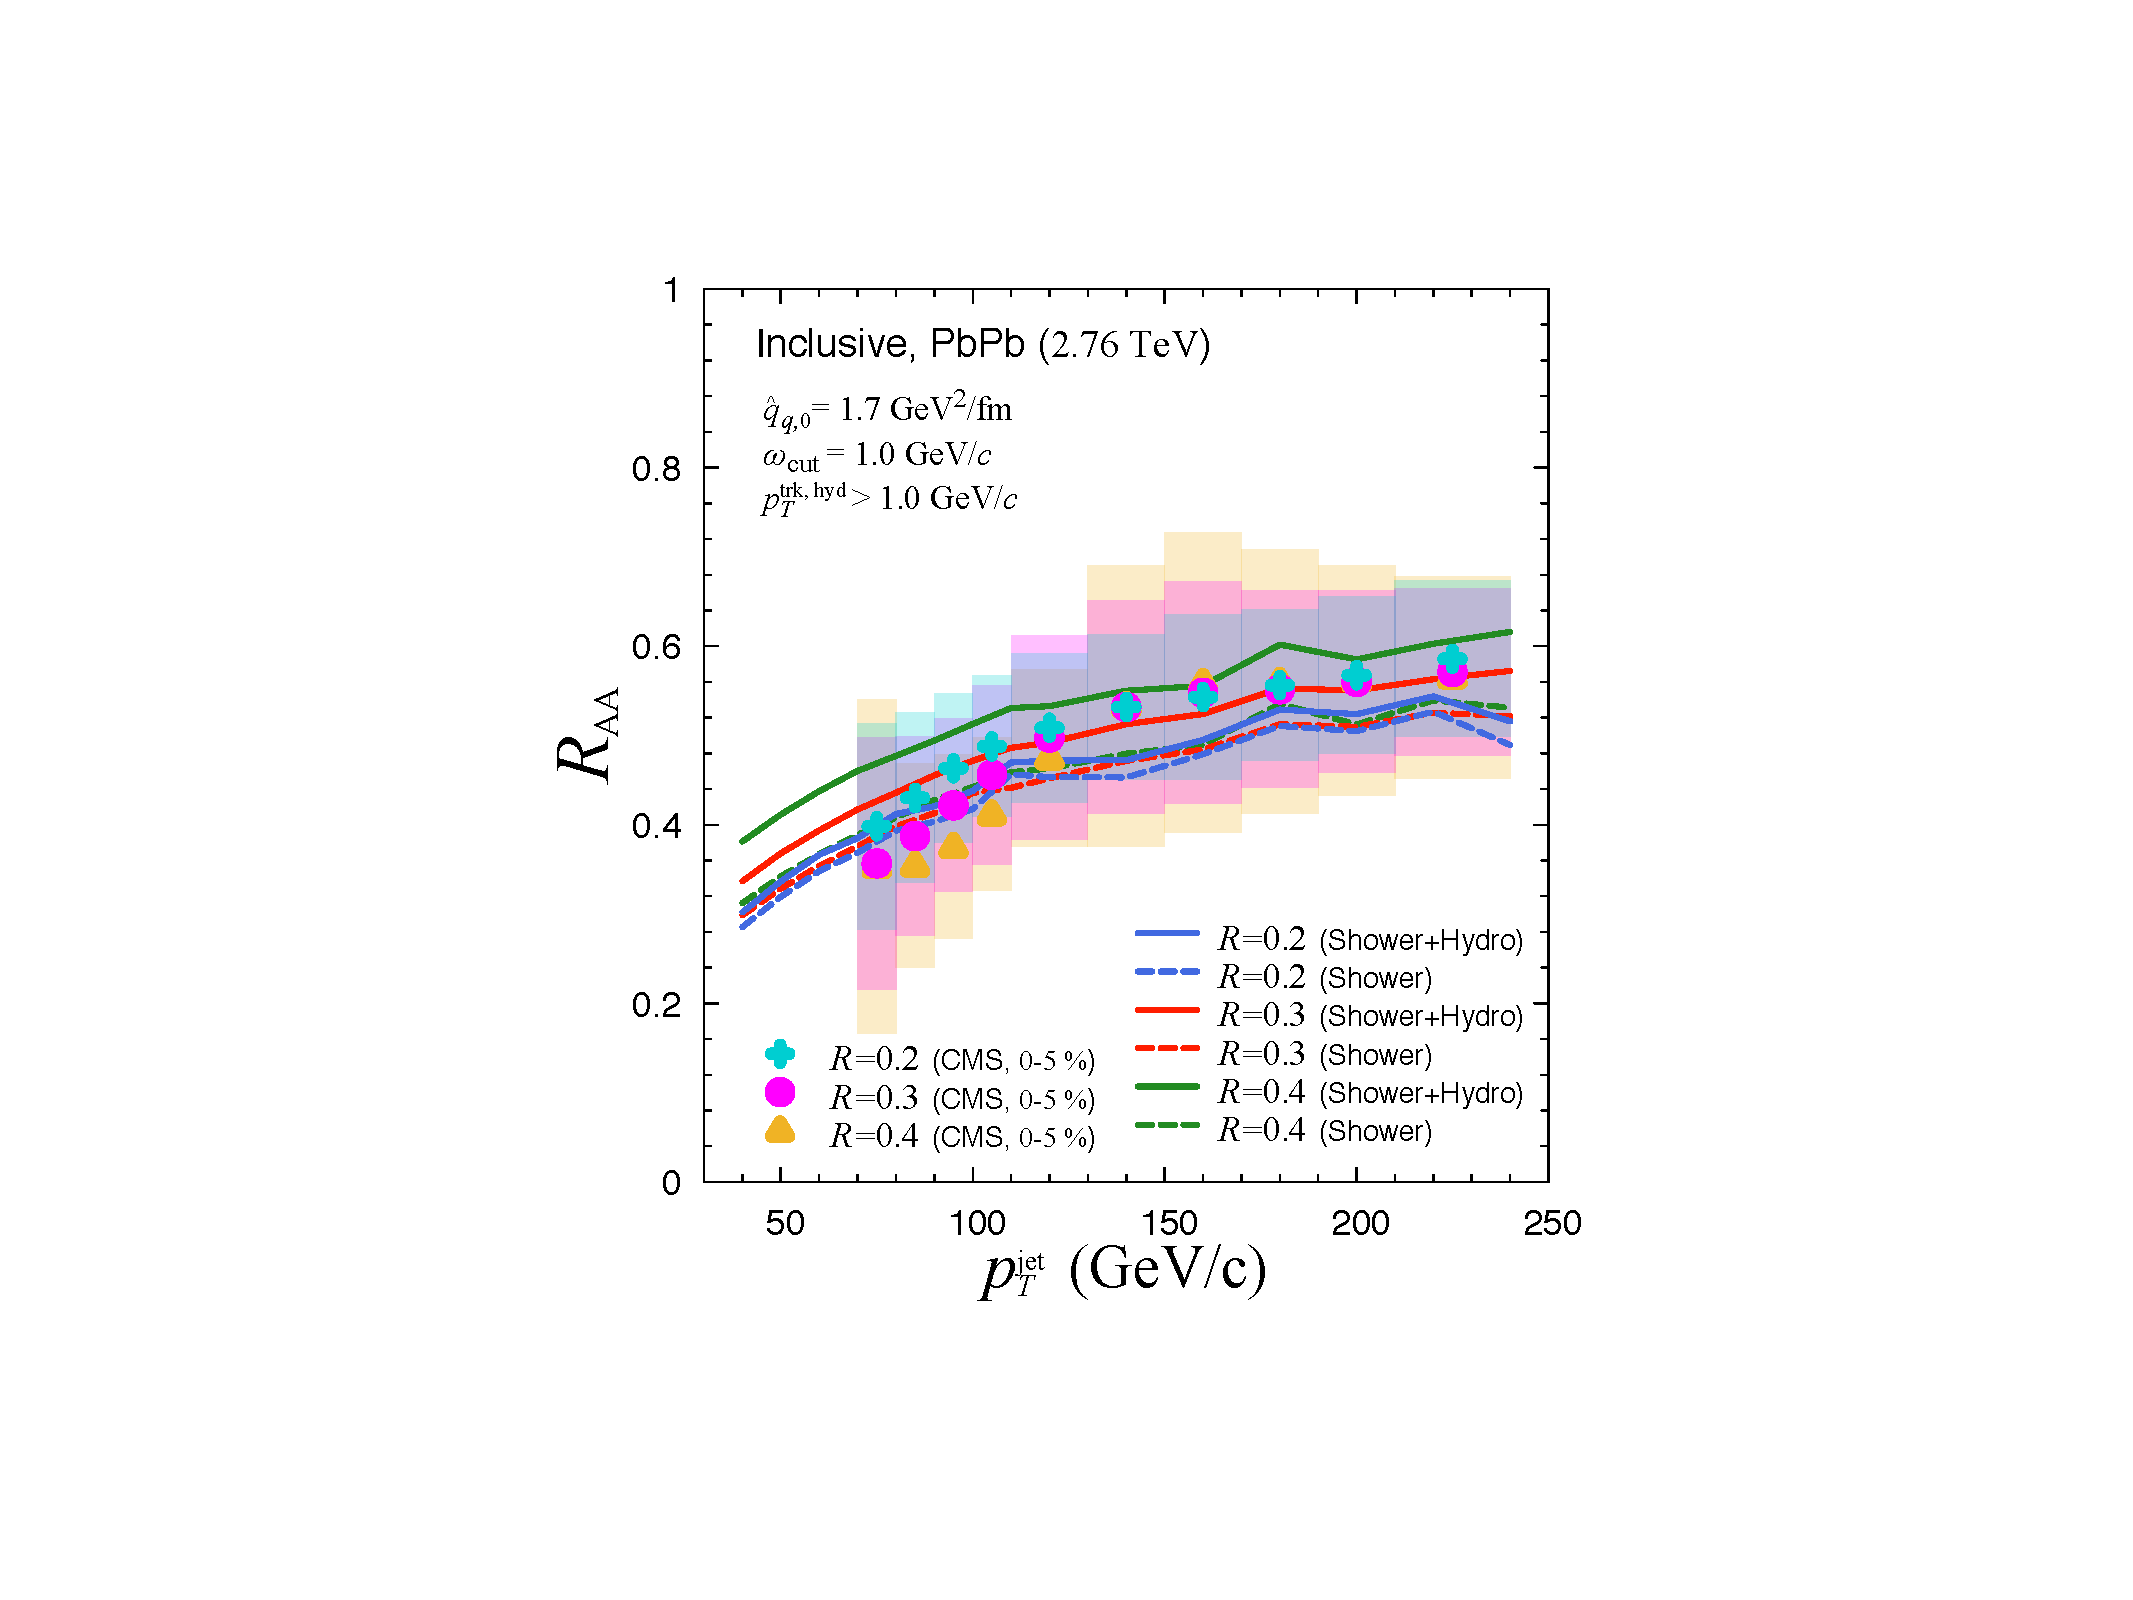
\includegraphics[width=0.45\textwidth]{figures/jetMeasurements/JF_RAA}
\caption{The nuclear modification factor \RAA\ as a function of jet \pt\ as determined by the Jet-Fluid model and compared to the data measured by CMS \cite{Khachatryan:2016jfl}. The different colors represent different sized jets, with the dashed lines showing the modeled \RAA\ without the hydro-contribution. There is good agreement within the large uncertainties in the data. Figure taken from \cite{Tachibana:2017syd}.}
\label{fig:jf_raa}
\end{center}
\end{figure}


The internal structure of the jet, i.e. how energy is spread within it, can be investigated using the jet shape variable, defined as a per-jet quantity as:

\begin{align}
\rho_{\rm jet} = \frac{1}{\Njet} \sum_{\rm jet} \left[ \frac{1}{\ptjet} \frac{\sum_{\rm trk} \pttrk}{\delta r}  \right]
\end{align}
where the sum is over all jets and for all tracks around a jet in an annulus with mean radius $r$ from the jet axis. The modification in the jet structure then can be defined as:

\begin{align}
R_{\rm AA}^\rho = \dfrac{\rho_{\rm AA} (r) }{\rho_{\rm pp} (r) }
\end{align}
A comparison of the jet shape variable $\rho$ and its modification $R_{\rm AA}^\rho$ to data measured by CMS is shown in Figure~\ref{fig:JF_jetShapemodel}. The individual shower and hydro contributions are seen in Figure~\ref{fig:jf_jetshape}. These indicate that the shower contribution to the jet shape variable is falls steeply as a function of distance from the jet axis while the hydro contribution is fairly constant at large distances. This is because the energy loss from the shower is carried away by the jet induced flow to large angles.
The $R_{\rm AA}^\rho$ distribution in Figure~\ref{fig:jf_jetshapemod}, shows that the core is largely unmodified while the outer part of the jet is broadened. The hydro-contribution mainly has an effect at larger distances from the jet axis. This is consistent with the cone-size dependence seen in Figure~\ref{fig:jf_energyLoss}.


\begin{figure}
\begin{subfigure}{.45\textwidth}
  \centering
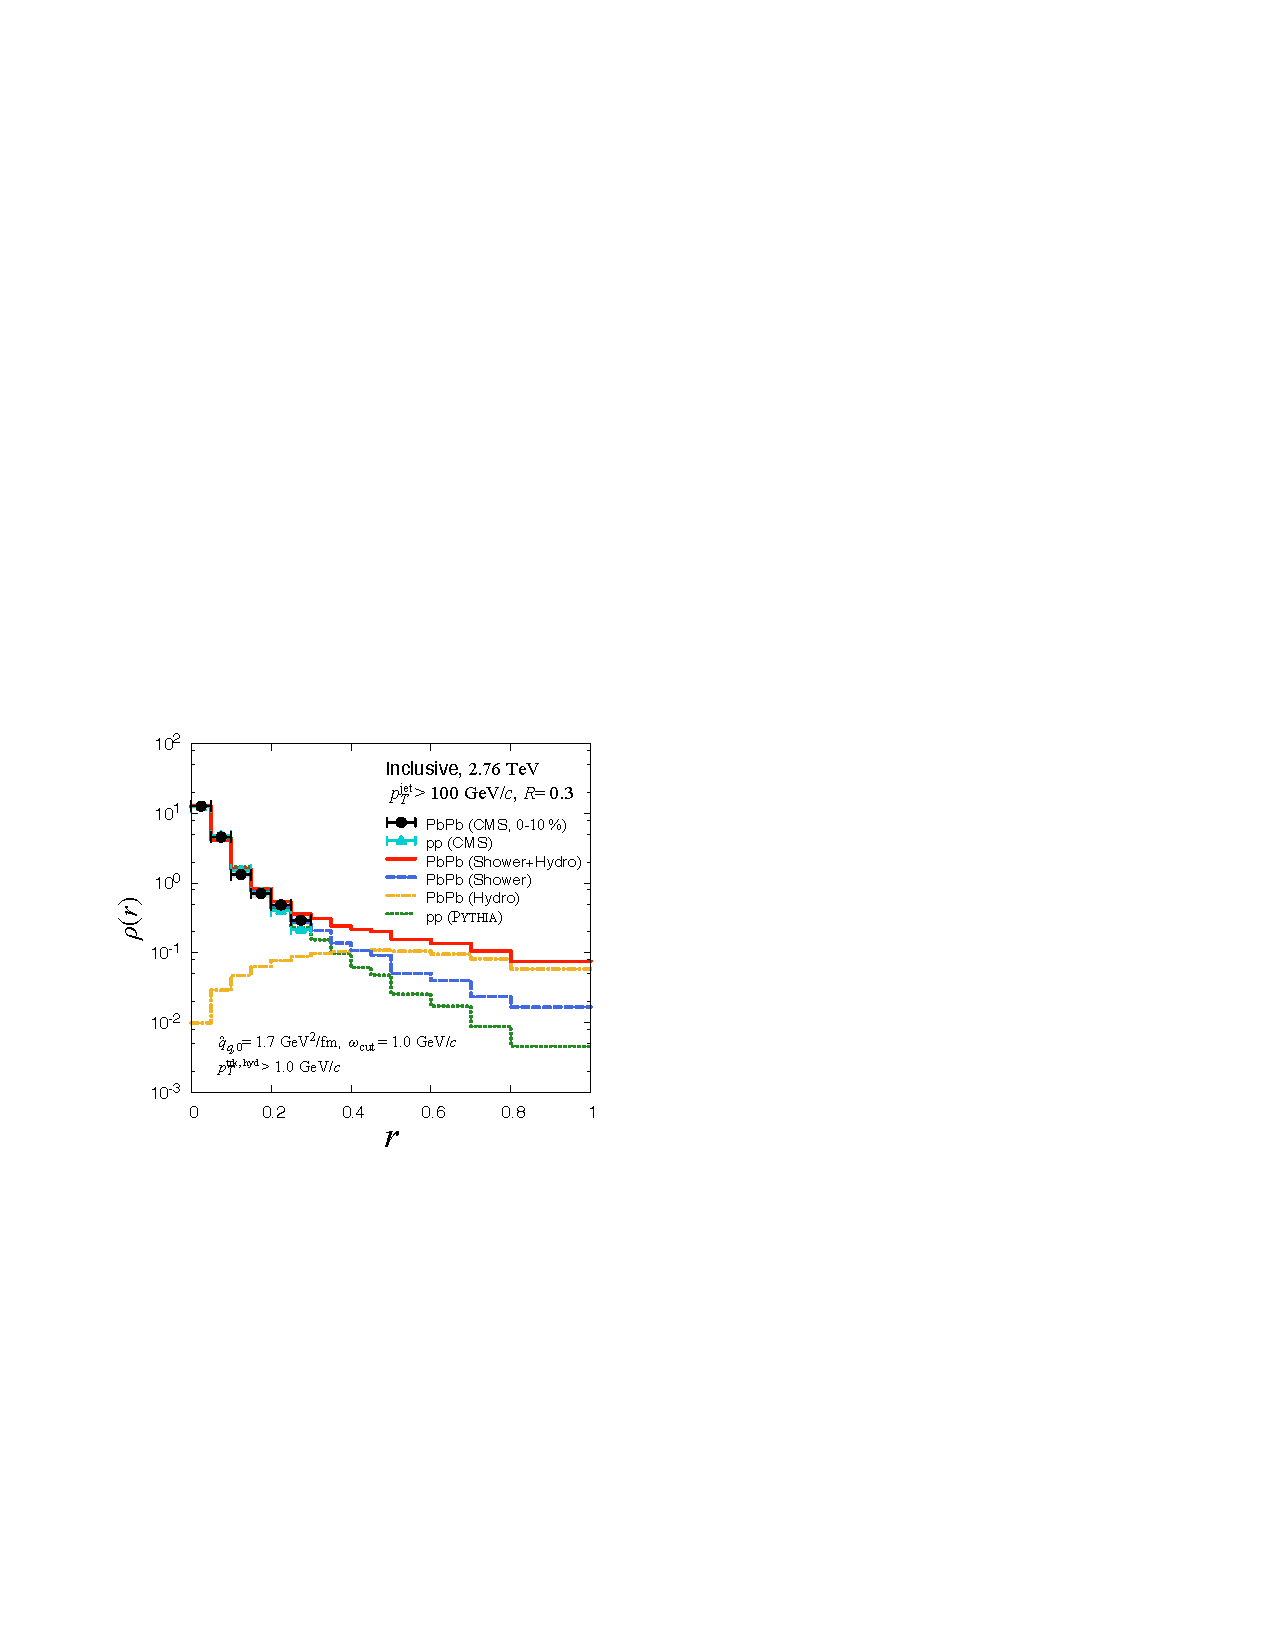
\includegraphics[width=0.95\textwidth]{figures/jetMeasurements/JF_jetShape}
\caption{The jet shape as measured by CMS for \pp\ and central \pbpb\ collisions \cite{Chatrchyan:2013kwa} compared to the Jet Fluid model. The shower (blue) and hydro (orange) contributions to the jet shape are highlighted.}
\label{fig:jf_jetshape}
\end{subfigure} \qquad
\begin{subfigure}{.45\textwidth}
  \centering
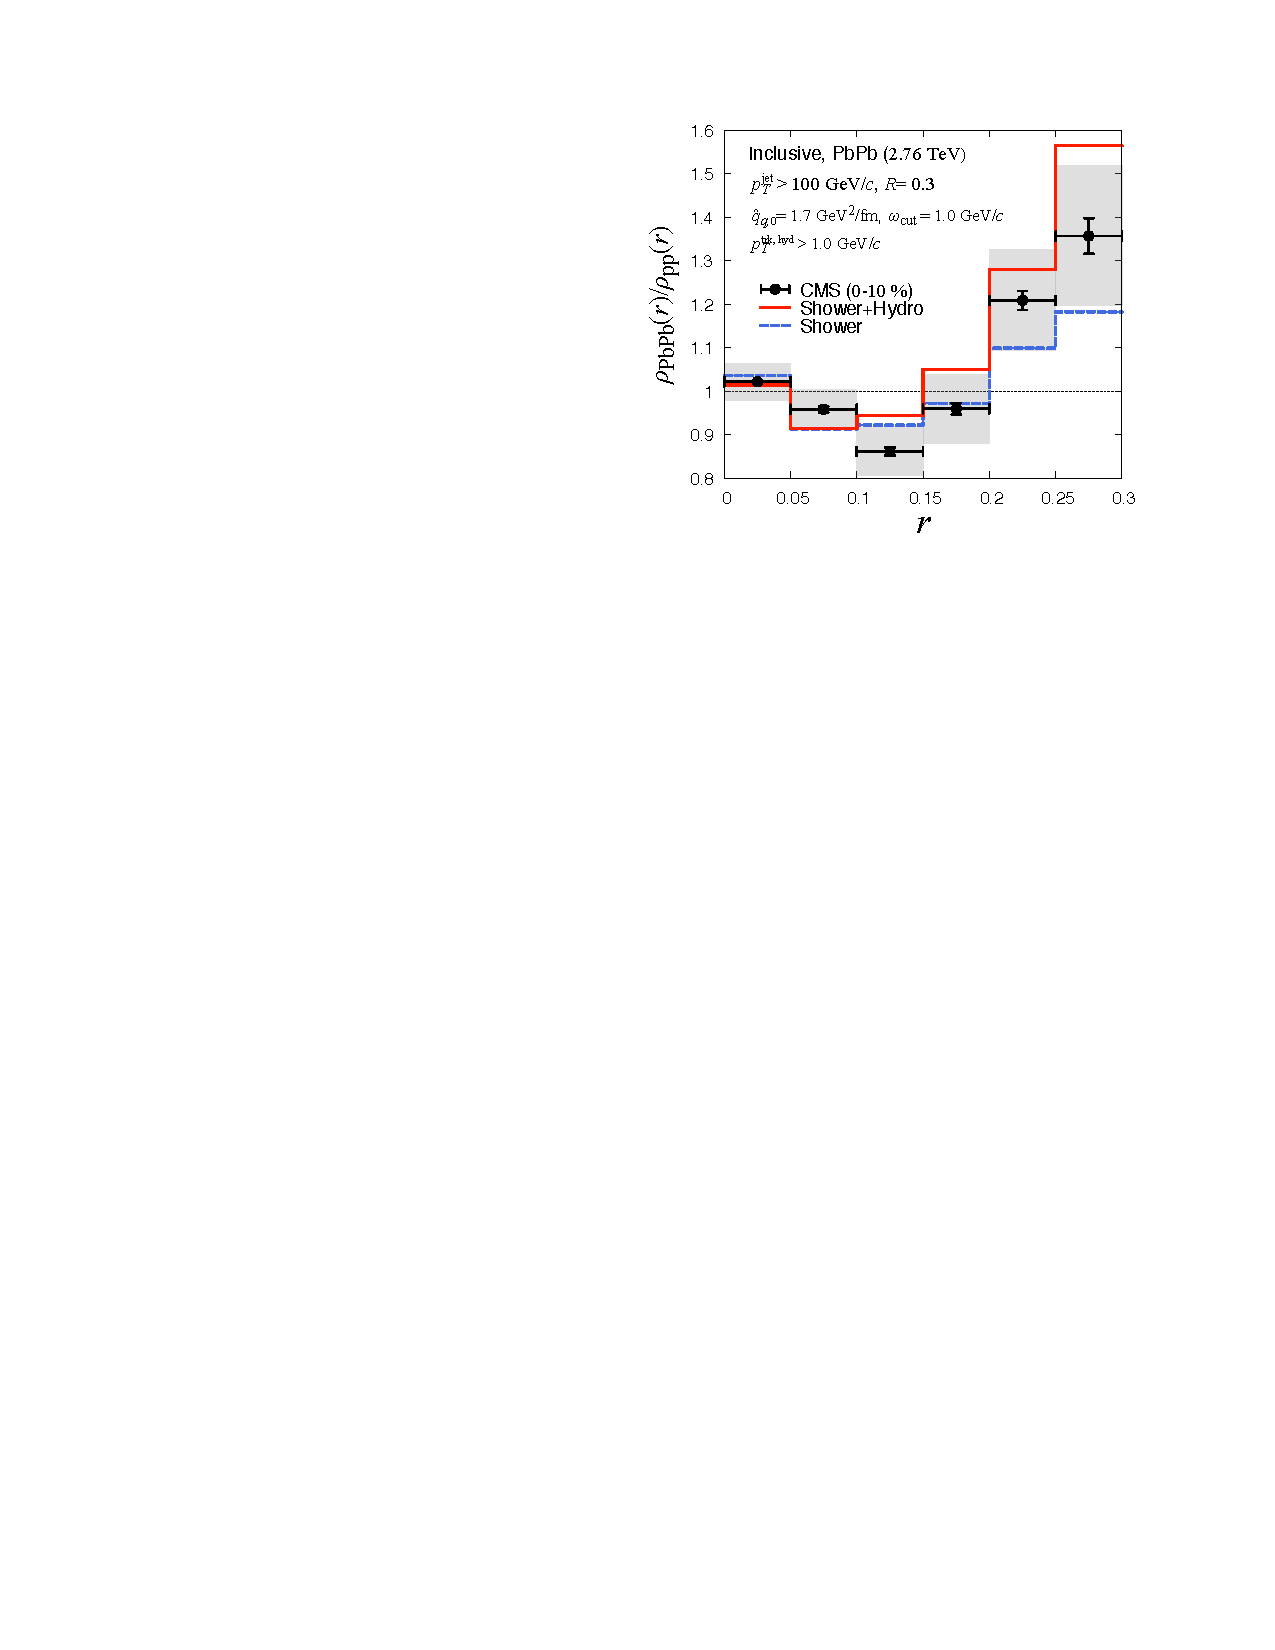
\includegraphics[width=0.95\textwidth]{figures/jetMeasurements/JF_jetShapeModification}
\caption{The modification of the jet shape between \pp\ and \pbpb\ as measured by CMS \cite{Chatrchyan:2013kwa} and compared to the Jet Fluid model. The dashed line shows the modeled modification without the hydro-contribution.}
\label{fig:jf_jetshapemod}
\end{subfigure}
\caption{Fits to CMS data. Figures taken from \cite{Tachibana:2017syd}.}
\label{fig:JF_jetShapemodel}
\end{figure}



%\begin{align}
%\frac{d f_j}{dt} =& \left( \hat{e_j} \frac{\p}{\p \omega_j} + \frac{1}{4} \hat{q_j} \nabla_{\kT}^2\right) f_j  \\
%& + \sum_i \int d\omega_i d\kTsq_i \frac{d\widetilde{\Gamma}_{i\rightarrow j} (\omega_j, \kTsq_j | \omega_i, \kTsq_i)}{d\omega_j d\kTsq dt} f_i \\
%& - \sum_i \int d\omega_i d\kTsq_i \frac{d\widetilde{\Gamma}_{j\rightarrow i} (\omega_i, \kTsq_i | \omega_j, \kTsq_j)}{d\omega_j d\kTsq dt} f_i \\
%\end{align}


%%%%%%%%%%%%%%%%%%%%%%%%%%%%%%%%%%%%%%
\section{Hybrid Model}
This discussion is based on the work in Refs. \cite{Casalderrey-Solana:2014bpa, Hulcher:2017cpt, Casalderrey-Solana:2016jvj} and describes jet quenching using a hybrid strong/weak model. It uses perturbative QCD to describe the weakly coupled hard process of jet production and holographic calculations of the energy loss of energetic probes to model the strong coupling between the probe and the plasma \cite{Chesler:2015nqz, Chesler:2014jva}. This is a combination of approaches that focus on the following extreme limits: a weakly coupled system at unrealistically high temperatures that can be treated perturbatively \cite{Jacobs:2004qv, Majumder:2010qh} and a system where the coupling constant is large at all energy scales and Gauge/string duality is applicable \cite{CasalderreySolana:2011us}.

In this model, the jet evolves in space time with the lifetime of the parton in the shower being given by \cite{CasalderreySolana:2011gx}.  

\begin{align}
\tau = 2 \frac{E}{Q^2}
\end{align}
where $Q$ is its virtuality and $E$ its energy. This evolution is unaffected before the proper time at which the plasma hydrodynamizes, $\tau_{\text{hydro}} = 0.6$ fm. After this time, the jet-plasma interaction comes into play and the fragments evolve with the energy loss as:

\begin{align}
\frac{1}{E_{\mathrm{in}}} \frac{dE}{dx} = -\frac{4}{\pi} \frac{x^2}{x_{\mathrm{stop}}^2} \frac{1}{\sqrt{x_{\mathrm{stop}}^2 - x^2}}
\end{align}
where $E_{\mathrm{in}}$ is the initial energy of the parton prior to any quenching and $x_{\mathrm{stop}}$ is its stopping distance (jet thermalization distance). The stopping distance can be written as:

\begin{align}
x_\mathrm{stop} = \frac{1}{2\kappa_\mathrm{sc}} \frac{E_\mathrm{in}^{1/3}}{T^{4/3}}
\end{align}
where $\kappa_\mathrm{sc}$ is a dimensionless free parameter associated to the strong coupling and is used to fit to the data. The energy loss is characterized by the strong  $x^2$ dependence for $x \ll x_\mathrm{stop}$. Furthermore, when $x$ is comparable to $x_\mathrm{stop}$, $dE/dx$ depends nontrivially on $E_\mathrm{in}$ and $x$, diverging for $x\rightarrow x_\mathrm{stop}$ and $E\rightarrow0$. The shower is then embedded into a hydrodynamic description of the QGP from Ref. \cite{Hirano:2010je}, and the energy loss expressions are integrated for each parton, from the time it is produced to the time that it splits. The splitting probabilities are taken to be independent of the medium, depending only on the initial energy of the daughter partons. These further lose energy as they propagate through the QGP and split. Then the total energy lost by a parton is dependent on the history of splitting and propagation of its parents, grandparents and so on and so forth. 

The partons further experience kicks transverse to their direction of motion, a phenomena called transverse momentum broadening. This effect is mainly experienced by softer partons that are much more affected by the angular narrowing effects of energy loss, making most measured observables insensitive to the size of this kick. This is directly related to wider jets losing more energy than narrower ones. The wake left in the medium from the partons depositing momentum in the QGP as they propagate through it lends a non-trivial impact to the model predictions. This wake moves in the direction of the jet and is impossible to separate out in experiments, making its inclusion to any model vital. This wake results in a perturbation to the hydrodynamic background, resulting in corrections to the final state hadron spectra. This effect is particularly important for jet substructure observables like jet fragmentation and jet shapes \cite{Casalderrey-Solana:2016jvj}.

A screening effect recently included in the hybrid model is based considering the resolving power of the QGP \cite{Hulcher:2017cpt}. As depicted in Figure~\ref{fig:hm_lres}, the QGP will only resolve daughter partons of a splitting after they are separated by a certain distance $L_\mathrm{res}$. It is only after they are resolved that they will be allowed them to lose energy independent of each other. This delayed quenching results in an enhancement of softer partons at larger angles from the jet axis compared to the case where the daughter partons are resolved immediately after they split from the parent parton. The \Lres\ parameter has the constraint $ 1/(\pi T) < \Lres < 2 /(\pt T$ based on the Debye screening length for the plasma, i.e. the length at which the QGP is able to resolve and screen color charges.

%The effects of including the \Lres parameter in the context of jet observables are discussed below.

\begin{figure}[htbp]
\begin{center}
\includegraphics[width=0.55\textwidth]{figures/jetMeasurements/HM_lres}
\caption{A schematic illustrating the resolving power of the QGP. The daughter partons $2$ and $3$ that come from $1$ need to be separated by \Lres\ before they are treated individually by the plasma. Prior to that separation, they are treated as one effective parton. Figure taken from \cite{Hulcher:2017cpt}.}
\label{fig:hm_lres}
\end{center}
\end{figure}


The free parameter $\kappa_\mathrm{sc}$ is determined by fitting to jet \RAA\ data from CMS \cite{Khachatryan:2016jfl} as shown in Figure~\ref{fig:hm_fitting}. It can be seen that including the \Lres\ parameter does not really affect the jet \RAA\ prediction. The dependence of the \RAA\ on the size of the jet radius can be seen. This is consistent with the expectation that wider jets lose more energy.

\begin{figure}[htbp]
\begin{center}
\includegraphics[width=1\textwidth]{figures/jetMeasurements/HM_raa}
\caption{The hybrid model without (left) and with (right) the \Lres\ parameter, compared to the jet \RAA\ as a function of jet \pt\ in two centrality intervals as measured in Ref. \cite{Khachatryan:2016jfl}. The different colors correspond to different jet radii. The Hybrid Model is fit to the 100--110 GeV point from the data, giving rise to the colored bands. Figure taken from \cite{Hulcher:2017cpt}. }
\label{fig:hm_fitting}
\end{center}
\end{figure}

Fixing the $\kappa_\mathrm{sc}$ parameter allows for predictions of other jet measurements like jet fragmentation and jet shape. Figures~\ref{fig:hm_ff} and \ref{fig:hm_jetshape} show a comparison of the measured and modeled values of the modifications to the jet fragmentation and jet shape respectively.  The model has also been compared to measurements done by ATLAS, ALICE, and STAR \cite{2013220, Abelev:2013kqa, RUSNAK:2014xfa} \cite{}


\begin{figure}
\begin{subfigure}{1\textwidth}
  \centering
\includegraphics[width=1\textwidth]{figures/jetMeasurements/HM_FF}
\caption{The modification to the jet fragmentation from \pp\ to \pbpb\ as a function of $\ln(1/z)$ as measured in Ref. \cite{Chatrchyan:2014ava} compared to the predictions of the hybrid model. The predictions are shown without (left) and with (right) the effect of the wake from the QGP responding to the jet. The different colors correspond to different \Lres\ parameters. Figure taken from \cite{Hulcher:2017cpt}. }
\label{fig:hm_ff}
\end{subfigure} \\ \\ \\
\begin{subfigure}{1\textwidth}
  \centering
\includegraphics[width=1\textwidth]{figures/jetMeasurements/HM_jetShape}
\caption{The modification to the jet shape from \pp\ to \pbpb\ as a function of $r$ as measured in Ref. \cite{Chatrchyan:2013kwa} compared to the predictions of the hybrid model. The predictions are shown without (left) and with (right) the effect of the wake from the QGP responding to the jet. The different colors correspond to different \Lres\ parameters. Figure taken from \cite{Hulcher:2017cpt}. }
\label{fig:hm_jetshape}
\end{subfigure}
\caption{A comparison of measured data, MC, and the analytic calculation of the EQ model. Figure taken from \cite{Spousta:2015fca}}
\label{fig:HM_modification}
\end{figure}


Here it can be seen that adding a medium response and a non-zero \Lres\ parameter affects the prediction. While the hard fragments (see Figure~\ref{}) are unaffected by the medium response, including the soft particles from the wake compensates some of the suppression of soft fragments in \pbpb\ compared to \pp\ collisions. Moreover, including the \Lres\ parameter further compensates the suppression for soft fragments, while reducing the enhancement of the hard fragments. This is a result of allowing more hadrons carrying a smaller fraction of the jet energy (low $z$, high ($\ln(1/z)$) to survive into the final state. The jet shape observable (see Figure~\ref{}) quantifies the radial distribution of energy in terms of annuli around the jet axis. It can be seen that introducing the \Lres\ parameter enhances the probability to find final state hadrons at larger distances from the jet axis. The jet core ($r < 0.05$) is also affected, with the depletion only slowly evolving with an increasing \Lres. One must be careful before making conclusions though, since these modifications are made between jets that are quenched (in \pbpb\ ) and unquenched (in \pp\ ). Taking into account the fact that wider jets lose more energy and that the jet spectrum rapidly falls off, there is a bias for finding narrower quenched jets than unquenched jets. This makes the jet shape after quenching narrower in \pbpb\ compared to \pp. While the model is not fully able to capture the features in the data, including the medium response moves it in the correct direction. It can be suggested that the model is missing a description of the medium induced modification to the hadronization process or that the wakes in the plasma are not equilibrating.










\clearpage

\chapter{JET ENERGY LOSS MODELS}
\label{sec:jetModels}
% !TEX encoding = UTF-8 Unicode
% !TEX root = thesis-ex.tex

While there are a number of different observables that can be measured in heavy ion collisions, the underlying goal of these measurements is to characterize the QGP.
This makes jet energy loss models that combine dynamics of the jet as well as the QGP invaluable.
Since different jet measurements come with their own set of measurement biases and have different sensitivities, it is vital that any viable model be able to describe a variety of observables.
Models can also help guide experimentalists in their searches and suggest new directions of exploration.
Measurements can then be done to constrain such models, helping further describe the jet-QGP interaction.

%In the case of jet energy loss, If a model can predict where the lost energy is redistributed, it is possible for experimentalists to measure an observable that would be sensitive to such effects, helping constrain the model.
%This sets up a healthy feedback loop between the theory and experiemnet communities.

%Mearuements of energy loss have to be coupled with models that describe the loss but also identify where the energy is redistributed. this makes measurements that are able to identify the different 
%Models investigating jet energy loss do not have to stop at just the loss, but also have to have a description of where the lost energy went.
%This makes models like the jet fluid model
%
%There is a constant feedback between the experimental measurements and models that attempt to describe them.
This chapter specifically discusses three different models: the Jet Fluid model, the Hybrid Model, and the Effective Quenching model.
These were chosen because they have been used to describe a wide variety of observables including the jet \RAA, jet fragmentation, and the jet shape.
In particular, the Jet Fluid model and Hybrid model incorporate a rigorous description of the interactions between the jet and the QGP and describe the radial dependence of the modification of charged particles in a jet, the central topic of this thesis. 
The Effective Quenching model is more phenomenological and shows agreement with measured data using only an intuitive functional form for energy loss.

\section{Jet Fluid model}
% !TEX encoding = UTF-8 Unicode
% !TEX root = thesis-ex.tex

This discussion is based on the model introduced in Ref.~\cite{Tachibana:2017syd}.
This model considers the evolution of the jet and QGP in a coupled manner, considering the energy and transverse momentum exchange between them.
In this picture, both the jet and medium are allowed to modify each other; the jet is modified via collisional and radiative processes while the medium evolves hydrodynamically and is modified because it picks up the energy lost by the jet.

The time evolution of the jet is given by a set of coupled transport equations that describe the energy and transverse momentum distributions of the partons within the jet. These are given as

\begin{gather}
f_i (\omega_i, \kTsq_i, t) = \frac{dN_i (\omega_i \kTsq_i, t)}{d \omega_i d\kTsq_i} \\
\nonumber \\
\frac{d f_j}{dt} = \hat{e_j} \frac{\p f_j}{\p \omega_j} + \frac{1}{4} \hat{q_j} \nabla_{\kT}^2 f_j 
 + \sum_i \int d\omega_i d\kTsq_i \frac{d\widetilde{\Gamma}_{i\rightarrow j} }{d\omega_j d\kTsq_j dt} f_i 
 - \sum_i \int d\omega_i d\kTsq_i \frac{d\widetilde{\Gamma}_{j\rightarrow i} }{d\omega_ij d\kTsq_i dt} f_i
\label{eq:jf_transportEq} 
\end{gather}
where $i$ is the type of parton, $\omega_i$ is its energy, and $\kTsq$ is its transverse momentum with respect to the jet axis.
The first term in Equation~\ref{eq:jf_transportEq} is the collisional energy loss, the second term is the transverse momentum broadening, and the last two terms are the medium induced gain and loss radiative processes respectively.
The splitting processes are are given by:

\begin{align}
\frac{d\Gamma_{i \rightarrow j}}{d \omega_j d\kTsq_j dt} = \frac{2\alpha_S}{\pi} \hat{q}_g \frac{x P_{i \rightarrow j} (x)}{\omega_j {k_{\rm T}^4}_j} \sin^2 \left(\dfrac{t - t_i}{2\tau_f} \right)
\end{align}
where $P_{i \rightarrow j} $ is the vacuum splitting function for $i \rightarrow j $ with $\omega_j$ being the energy of the radiated parton, $\tau_f$ is the formation time of the radiated parton, and $\kT_j$ is the transverse momentum of the radiated parton with respect to the parent parton.
These transport Equations~\ref{eq:jf_transportEq} can be solved numerically and agree with \RAA\ measurements \cite{Aad:2014bxa, Khachatryan:2016jfl, Abelev:2013kqa}.
The effects of the medium are included by considering the energy-momentum conservation of the jet-QGP system $ \p_\mu [T_{\rm QGP}^{\mu\nu} + T_{\rm jet}^{\mu\nu}] = 0$.
Then the source term $J^\nu(x)$ that describes the energy transfer between the jet and the medium can be defined as $J^\nu(x) \equiv -\p_\mu  T_{\rm jet}^{\mu\nu}$, making the QGP evolution being given by

\begin{align}
 \p_\mu T_{\rm QGP}^{\mu\nu} = j^\nu
\end{align}
which characterizes the energy-momentum transfer between the jet and the QGP.

An important component of this model is the flow induced by jets.
This can be seen in Figure~\ref{fig:jf_snapshot}, where the evolution of the energy density of the medium can be seen in a sample event.
A single jet travels through the QGP, and can be clearly seen in the lower panels after the energy of the medium has been subtracted out.
The ``V'' shaped feature seen is the mach cone that is induced by the parton as it moves faster than the medium sound velocity.


\begin{figure}[htbp]
\begin{center}
\includegraphics[width=0.85\textwidth]{figures/jetMeasurements/JF_snapshot}
\caption{(Top) The time evolution of the energy density of the quark gluon plasma with a jet propagating through it.
(Bottom) The time evolution of the energy density in the event after the energy density of the QGP has been subtracted out.
Figure taken from \cite{Tachibana:2017syd}.}
\label{fig:jf_snapshot}
\end{center}
\end{figure}

The final jet energy has two components: the jet shower, and the hydrodynamic response.
The former as discussed above comprises of the collisional energy loss, momentum broadening, and medium induced radiation.
The latter includes the energy lost from the jet shower that thermalizes into the medium and induces conical flow, some of which is still in the jet cone.
This compensates some of the energy lost in the shower and can be seen in Figure~\ref{fig:jf_energyLoss}.
While the absolute amount of energy lost increases as a function of initial jet energy, the fractional energy loss decreases.
Furthermore there is a cone size dependence once the hydrodynamic contributions are included.
This is a result of the jet being highly collimated, such that while an increase in the size does not change the energy much, it does affect the hydrodynamic contribution from the medium.


\begin{figure}
\begin{center}
  \begin{minipage}[b]{0.43\textwidth}
\includegraphics[ width=\textwidth]{figures/jetMeasurements/JF_energyLoss}
\caption{(Top) The energy lost by a jets of different radii as a function of their initial energy in central \pbpb\ collisions at \sqrtsnn = 2.76 TeV.
Figure taken from \cite{Tachibana:2017syd}.}
\label{fig:jf_energyLoss}
  \end{minipage}
 \qquad  \qquad  \qquad
  \begin{minipage}[b]{0.43\textwidth}
\includegraphics[width=\textwidth]{figures/jetMeasurements/JF_RAA}
\caption{The jet \RAA\ measured by CMS \cite{Khachatryan:2016jfl} and compared to the Jet-Fluid model with and without the hydro dynamic contribution.
Figure taken from \cite{Tachibana:2017syd}.}
\label{fig:jf_raa}
  \end{minipage}
  \end{center}
\end{figure}



%\begin{figure}[htbp]
%\begin{center}
%\includegraphics[width=0.45\textwidth]{figures/jetMeasurements/JF_energyLoss}
%\caption{(Top) The energy lost by a jets of different radii as a function of their initial energy in central \pbpb\ collisions at \sqrtsnn = 2.76 TeV.
%Figure taken from \cite{Tachibana:2017syd}.}
%\label{fig:jf_energyLoss}
%\end{center}
%\end{figure}

The \RAA\ distributions constructed with this model and compared to data from CMS \cite{Khachatryan:2016jfl} are shown in Figure~\ref{fig:jf_raa}.
Including the hydrodynamic contribution decreases the energy loss, hence increasing the \RAA\ value and inducing a cone size dependence to the \RAA.

%\begin{figure}[htbp]
%\begin{center}
%\includegraphics[width=0.45\textwidth]{figures/jetMeasurements/JF_RAA}
%\caption{The nuclear modification factor \RAA\ as a function of jet \pt\ as determined by the Jet-Fluid model and compared to the data measured by CMS \cite{Khachatryan:2016jfl}.
%The different colors represent different sized jets, with the dashed lines showing the modeled \RAA\ without the hydro-contribution.
%There is good agreement within the large uncertainties in the data.
%Figure taken from \cite{Tachibana:2017syd}.}
%\label{fig:jf_raa}
%\end{center}
%\end{figure}

The internal structure of the jet can be described using the jet shape variable, defined as a per-jet quantity as:

\begin{align}
\rho_{\rm jet} = \frac{1}{\Njet} \sum_{\rm jet} \left[ \frac{1}{\ptjet} \frac{\sum_{\rm trk} \pttrk}{\delta r}  \right]
\end{align}
where the sum is over all jets and for all tracks around a jet in an annulus with mean radius $r$ from the jet axis.
The modification in the jet structure then can be defined as $R_{\rm AA}^\rho = \rho_{\rm AA} (r) / \rho_{\rm pp} (r) $.
%
%\begin{align}
%R_{\rm AA}^\rho = \dfrac{\rho_{\rm AA} (r) }{\rho_{\rm pp} (r) }
%\end{align}
A comparison of the jet shape variable $\rho$ and its modification $R_{\rm AA}^\rho$ to data measured by CMS is shown in Figure~\ref{fig:JF_jetShapemodel}.
The individual shower and hydro contributions are seen in Figure~\ref{fig:jf_jetshape}.
These indicate that the shower contribution to the jet shape variable is falls steeply as a function of distance from the jet axis while the hydro contribution is fairly constant at large distances.
This is because the energy loss from the shower is carried away by the jet induced flow to large angles.
The $R_{\rm AA}^\rho$ distribution in Figure~\ref{fig:jf_jetshapemod}, shows that the core is largely unmodified while the outer part of the jet is broadened.
The hydro-contribution mainly has an effect at larger distances from the jet axis.
This is consistent with the cone-size dependence seen in Figure~\ref{fig:jf_energyLoss}.


\begin{figure}
\begin{subfigure}{.45\textwidth}
  \centering
\includegraphics[width=0.95\textwidth]{figures/jetMeasurements/JF_jetShape}
\caption{The jet shape as measured by CMS for \pp\ and central \pbpb\ collisions \cite{Chatrchyan:2013kwa} compared to the Jet Fluid model.
The shower (blue) and hydro (orange) contributions to the jet shape are highlighted.}
\label{fig:jf_jetshape}
\end{subfigure} \qquad
\begin{subfigure}{.45\textwidth}
  \centering
\includegraphics[width=0.95\textwidth]{figures/jetMeasurements/JF_jetShapeModification}
\caption{The modification of the jet shape between \pp\ and \pbpb\ as measured by CMS \cite{Chatrchyan:2013kwa} and compared to the Jet Fluid model.
The dashed line shows the modeled modification without the hydro-contribution.}
\label{fig:jf_jetshapemod}
\end{subfigure}
\caption{Fits to CMS data.
Figures taken from \cite{Tachibana:2017syd}.}
\label{fig:JF_jetShapemodel}
\end{figure}



%\begin{align}
%\frac{d f_j}{dt} =& \left( \hat{e_j} \frac{\p}{\p \omega_j} + \frac{1}{4} \hat{q_j} \nabla_{\kT}^2\right) f_j  \\
%& + \sum_i \int d\omega_i d\kTsq_i \frac{d\widetilde{\Gamma}_{i\rightarrow j} (\omega_j, \kTsq_j | \omega_i, \kTsq_i)}{d\omega_j d\kTsq dt} f_i \\
%& - \sum_i \int d\omega_i d\kTsq_i \frac{d\widetilde{\Gamma}_{j\rightarrow i} (\omega_i, \kTsq_i | \omega_j, \kTsq_j)}{d\omega_j d\kTsq dt} f_i \\
%\end{align}

\label{sec:jet_fluid}

\section{Hybrid Model}
% !TEX encoding = UTF-8 Unicode
% !TEX root = thesis-ex.tex

This discussion is based on the work in Refs.~\cite{Casalderrey-Solana:2014bpa, Hulcher:2017cpt, Casalderrey-Solana:2016jvj} and describes jet quenching using a hybrid strong/weak model.
It uses perturbative QCD to describe the weakly coupled hard process of jet production and holographic calculations of the energy loss of energetic probes to model the strong coupling between the probe and the plasma \cite{Chesler:2015nqz, Chesler:2014jva}.
This is a combination of approaches that focus on the following extreme limits: a weakly coupled system at unrealistically high temperatures that can be treated perturbatively \cite{Jacobs:2004qv, Majumder:2010qh} and a system where the coupling constant is large at all energy scales and Gauge/string duality is applicable \cite{CasalderreySolana:2011us}.
In this model, the jet evolves in space time with the lifetime of the parton in the shower being given by \cite{CasalderreySolana:2011gx}.
 

\begin{align}
\tau = 2 \frac{E}{Q^2}
\end{align}
where $Q$ is its virtuality and $E$ its energy.
This evolution is unaffected before the proper time at which the plasma hydrodynamizes, $\tau_{\text{hydro}} = 0.6$ fm.
After this time, the jet-plasma interaction comes into play and the fragments evolve with the energy loss as:

\begin{align}
\frac{1}{E_{\mathrm{in}}} \frac{dE}{dx} = -\frac{4}{\pi} \frac{x^2}{x_{\mathrm{stop}}^2} \frac{1}{\sqrt{x_{\mathrm{stop}}^2 - x^2}}
\end{align}
where $E_{\mathrm{in}}$ is the initial energy of the parton prior to any quenching and $x_{\mathrm{stop}}$ is its stopping distance (jet thermalization distance).
The stopping distance can be written as:

\begin{align}
x_\mathrm{stop} = \frac{1}{2\kappa_\mathrm{sc}} \frac{E_\mathrm{in}^{1/3}}{T^{4/3}}
\end{align}
where $\kappa_\mathrm{sc}$ is a dimensionless free parameter associated to the strong coupling and is used to fit to the data.

The energy loss is characterized by the strong  $x^2$ dependence for $x \ll x_\mathrm{stop}$.
Furthermore, when $x$ is comparable to $x_\mathrm{stop}$, $dE/dx$ depends nontrivially on $E_\mathrm{in}$ and $x$, diverging for $x\rightarrow x_\mathrm{stop}$ and $E\rightarrow0$.
The shower is then embedded into a hydrodynamic description of the QGP from Ref.
\cite{Hirano:2010je}, and the energy loss expressions are integrated for each parton, from the time it is produced to the time that it splits.
The splitting probabilities are taken to be independent of the medium, depending only on the initial energy of the daughter partons.
These further lose energy as they propagate through the QGP and split.
Then the total energy lost by a parton is dependent on the history of splitting and propagation of its parents, grandparents and so on and so forth.
The partons further experience kicks transverse to their direction of motion, a phenomena called transverse momentum broadening.
This effect is mainly experienced by softer partons that are much more affected by the angular narrowing effects of energy loss, making most measured observables insensitive to the size of this kick.
This is directly related to wider jets losing more energy than narrower ones.
The wake left in the medium from the partons depositing momentum in the QGP as they propagate through it lends a non-trivial impact to the model predictions.
It is a vital part of any model since the contribution from the wake is impossible to separate experimentally. 
This wake results in a perturbation to the hydrodynamic background resulting in corrections to the final state hadron spectra, making it particularly important for jet substructure observables like jet fragmentation and jet shapes \cite{Casalderrey-Solana:2016jvj}.

A screening effect recently included in the hybrid model is based considering the resolving power of the QGP \cite{Hulcher:2017cpt}.
As depicted in Figure~\ref{fig:hm_lres}, the QGP will only resolve daughter partons of a splitting after they are separated by a certain distance $L_\mathrm{res}$.
It is only after they are resolved that they will be allowed them to lose energy independent of each other.
This delayed quenching results in an enhancement of softer partons at larger angles from the jet axis compared to the case where the daughter partons are resolved immediately after they split from the parent parton.
The \Lres\ parameter has the constraint $ 1/(\pi T) < \Lres < 2 /(\pt T$ based on the Debye screening length for the plasma.

%The effects of including the \Lres parameter in the context of jet observables are discussed below.

\begin{figure}[htbp]
\begin{center}
\includegraphics[width=0.55\textwidth]{figures/jetMeasurements/HM_lres}
\caption{A schematic illustrating the resolving power of the QGP.
The daughter partons $2$ and $3$ that come from $1$ need to be separated by \Lres\ before they are treated individually by the plasma.
Prior to that separation, they are treated as one effective parton.
Figure taken from \cite{Hulcher:2017cpt}.}
\label{fig:hm_lres}
\end{center}
\end{figure}


The free parameter $\kappa_\mathrm{sc}$ is determined by fitting to jet \RAA\ data from CMS \cite{Khachatryan:2016jfl} as shown in Figure~\ref{fig:hm_fitting}.
It can be seen that including the \Lres\ parameter does not really affect the jet \RAA\ prediction.
The dependence of the \RAA\ on the size of the jet radius can be seen.
This is consistent with the expectation that wider jets lose more energy.

\begin{figure}[htbp]
\begin{center}
\includegraphics[width=1\textwidth]{figures/jetMeasurements/HM_raa}
\caption{The hybrid model without (left) and with (right) the \Lres\ parameter, compared to the jet \RAA\ as a function of jet \pt\ in two centrality intervals as measured in Ref.
\cite{Khachatryan:2016jfl}.
The different colors correspond to different jet radii.
The Hybrid Model is fit to the 100--110 GeV point from the data, giving rise to the colored bands.
Figure taken from \cite{Hulcher:2017cpt}.
}
\label{fig:hm_fitting}
\end{center}
\end{figure}

Fixing the $\kappa_\mathrm{sc}$ parameter allows for predictions of other jet measurements like jet fragmentation and jet shape.
Figures~\ref{fig:hm_ff} and \ref{fig:hm_jetshape} show a comparison of the measured and modeled values of the modifications to the jet fragmentation and jet shape respectively.
 The model has also been compared to measurements done by ATLAS, ALICE, and STAR \cite{2013220, Abelev:2013kqa, RUSNAK:2014xfa}


\begin{figure}
\begin{subfigure}{1\textwidth}
  \centering
\includegraphics[width=1\textwidth]{figures/jetMeasurements/HM_FF}
\caption{The modification to the jet fragmentation from \pp\ to \pbpb\ as a function of $\ln(1/z)$ as measured in Ref.
\cite{Chatrchyan:2014ava} compared to the predictions of the hybrid model.
The predictions are shown without (left) and with (right) the effect of the wake from the QGP responding to the jet.
The different colors correspond to different \Lres\ parameters.
Figure taken from \cite{Hulcher:2017cpt}.}
\label{fig:hm_ff}
\end{subfigure} \\ \\ \\
\begin{subfigure}{1\textwidth}
  \centering
\includegraphics[width=1\textwidth]{figures/jetMeasurements/HM_jetShape}
\caption{The modification to the jet shape from \pp\ to \pbpb\ as a function of $r$ as measured in Ref.
\cite{Chatrchyan:2013kwa} compared to the predictions of the hybrid model.
The predictions are shown without (left) and with (right) the effect of the wake from the QGP responding to the jet.
The different colors correspond to different \Lres\ parameters.
Figure taken from \cite{Hulcher:2017cpt}.}
\label{fig:hm_jetshape}
\end{subfigure}
\caption{A comparison of measured data, MC, and the analytic calculation of the EQ model.
Figure taken from \cite{Spousta:2015fca}}
\label{fig:HM_modification}
\end{figure}


Here it can be seen that adding a medium response and a non-zero \Lres\ parameter affects the prediction.
While the hard fragments (see Figure~\ref{fig:hm_ff}) are unaffected by the medium response, including the soft particles from the wake compensates some of the suppression of soft fragments in \pbpb\ compared to \pp\ collisions.
Moreover, including the \Lres\ parameter further compensates the suppression for soft fragments, while reducing the enhancement of the hard fragments.
This is a result of allowing more hadrons carrying a smaller fraction of the jet energy (low $z$, high ($\ln(1/z)$) to survive into the final state.
The jet shape observable (see Figure~\ref{fig:hm_jetshape}) quantifies the radial distribution of energy in terms of annuli around the jet axis.
It can be seen that introducing the \Lres\ parameter enhances the probability to find final state hadrons at larger distances from the jet axis.
The jet core ($r < 0.05$) is also affected, with the depletion only slowly evolving with an increasing \Lres.
One must be careful before making conclusions though, since these modifications are made between jets that are quenched (in \pbpb\ ) and unquenched (in \pp\ ).
Taking into account the fact that wider jets lose more energy and that the jet spectrum rapidly falls off, there is a bias for finding narrower quenched jets than unquenched jets.
This makes the jet shape after quenching narrower in \pbpb\ compared to \pp.
While the model is not fully able to capture the features in the data, including the medium response moves it in the correct direction.
It can be suggested that the model is missing a description of the medium induced modification to the hadronization process or that the wakes in the plasma are not equilibrating.










\label{sec:hybrid_model}

\section{Effective Quenching}
% !TEX encoding = UTF-8 Unicode
% !TEX root = thesis-ex.tex

This discussion is based on the model introduced in Ref.
\cite{Spousta:2015fca}.
This phenomenological model emphasizes the jet \pt\ dependence of the quark to gluon fraction and the difference between quark-jet and gluon-jet quenching.
It uses an ``extended'' power law parameterization of the high-\pt\ hadron spectra coupled with a quenching that is based on a non-constant fractional energy loss.
This model considers the different color charges carried by quarks and gluons and their different splitting functions, and assumes that gluon jets lose energy at a rate 9/4 times higher than quark jets.
The key assumption of the model are:
\begin{itemize}
\item The energy lost by a jet is radiated at large angles and does not appear within the jet cone.
This is backed by \cite{Chatrchyan:2011sx}.
\item The fragmentation pattern of the jet is unaffected by the presence of the QGP i.e.
they fragment as they would in a vacuum.
This is motivated by the idea that the QGP is unable to resolve the internal jet structure and is supported by \cite{Blaizot:2013hx, CasalderreySolana:2012ef}.
\end{itemize} 

The model uses the following extended power-law parameterization to describe the high-\pt\ jet spectra:

\begin{align}
\frac{dn}{d\ptjet} = A \left( \frac{\pt_0}{\ptjet} \right) ^{n+\beta \log(\ptjet / \pt_0)}
\label{eq:eq_spectrum}
\end{align}
where $\pt_0$ is a reference transverse momentum at which $A= dn/d\ptjet$, $\beta$ is the logarithmic derivative of $dn/d\ptjet$ at $\ptjet = \pt_0$.
Then the combined spectrum from quarks and gluons can be written in terms of Equation~\ref{eq:eq_spectrum} with weighted contributions from the different quark and gluon fractions, $f_{q0}$ and $f_{g0} = 1-f_{q0}$ respectively.

%\begin{align}
% \frac{dN}{d\ptjet} &= A \left[ f_{q0} \left( \frac{\pt_0}{\ptjet} \right)^{n_q+ \beta_q \log(\ptjet / \pt_0)} + (1-f_{q0}) \left( \frac{\pt_0}{\ptjet} \right)^{n_g + \beta_g \log(\ptjet / \pt_0)} \right] \\
%\nonumber \\ 
%\label{eq:eq_q_frac} f_q (\ptjet) &= \dfrac{1}{1 + \left(\dfrac{1-f_{q0}}{f_{q0}}\right) \left( \dfrac{\pt_0}{\ptjet}\right)^{\Delta n + \Delta \beta \log(\ptjet/\pt_0)} }
%\end{align}
%where $\Delta n = n_g - n_q$ and $\Delta \beta = \beta_g - \beta_q$.
The \pt\ dependence of the quark fraction along with the fit is shown in Figure~\ref{fig:eq_raa_centDep}.
The fragmentation functions can also be determined using final-state charged hadrons within a $R=0.4$ jet cone.
These are fit to the form \Dz, with fits for the quark and gluon fragmentation shown in Figure~\ref{fig:gluon_fragmentation}.


\begin{align}
D(z) = a \times \frac{(1+dz)^b}{(1+ez)^c} \times e^{-fz}
\label{eq:ff_param}
\end{align}


\begin{figure}
\begin{subfigure}{.45\textwidth}
  \centering
\includegraphics[width=0.8\textwidth]{figures/jetMeasurements/jetQuarkFraction}
\caption{The jet quark fraction as a function of \ptjet\ in different rapidity bins.
The points are from \pythia8 simulations and the lines are fits to the spectra determined using Equation~\ref{eq:eq_spectrum}.}
\label{fig:eq_raa_centDep}
\end{subfigure} \qquad
\begin{subfigure}{.45\textwidth}
  \centering
\includegraphics[width=0.8\textwidth]{figures/jetMeasurements/gluon_fragmentation}
\caption{A comparison of the quark and gluon fragmentation.
The points are from \pythia8 simulations and the lines are fits to those points using Equation~\ref{eq:ff_param}.}
\label{fig:gluon_fragmentation}
\end{subfigure}
\caption{Fits to quark fractions and fragmentation functions from \pythia8.
 Figure taken from \cite{Spousta:2015fca}.}
\label{fig:EQ_pp_models}
\end{figure}

For the quenched spectra, this model assumes a non-constant fractional shift given below as $S$.
This approach is based on \cite{baier2001quenching} and is used because of the inability of the constant fractional shift to explain the jet \pt\ dependence of measured \RAA.

\begin{align}
S = s' \left( \frac{\ptjet}{\pt_0} \right) ^\alpha
\end{align}
where $\alpha$ is an undetermined parameter and $s'$ is the shift for a jet with $\ptjet = \pt_0$.
The fractional shift can be coupled with Equation~\ref{eq:eq_spectrum} and the quark and gluon fractions to give a functional form of the quenched high-\pt\ hadron spectra for quarks and gluons.
This can be further used to construct a jet \RAA\ that is fit to data and is shown in Figure~\ref{fig:EQ_RAA}.
It can be seen that the analytic fits and the MC are in good agreement.
While the fits agree with the data by definition, the robustness of the model can be seen in that it describes the data with a single value for $\alpha$ and a simple centrality dependent shift constant $s'$.


%\begin{align}
% \frac{dN_Q}{d\ptjet} &= A \Bigg[ f_{q0} \left( \frac{\pt_0}{\ptjet+S_q} \right)^{n_q+ \beta_q \log\big((\ptjet+S_q) / \pt_0\big)} \left(1 + \frac{dS_q}{d\ptjet} \right) \\
%& + (1-f_{q0}) \left( \frac{\pt_0}{\ptjet+S_g} \right)^{n_g + \beta_g \log\big((\ptjet+S_g) / \pt_0\big)}  \left(1 + \frac{dS_g}{d\ptjet} \right) \Bigg] \nonumber
%\end{align}
%Where the $(1+dS/d\ptjet)$ term is a Jacobian to preserve the number of jets.
%Then the \RAA\ can be written as:
%\begin{align}
%\RAA = f_q & \left(\frac{1}{1 + S_q / \ptjet}\right) ^{n_q + \beta_q \log\big((\ptjet+S_q)/\pt_0\big)}  \frac{\pt_0}{\ptjet}^{} \left( 1+ \frac{dS_q}{d\ptjet} \right) \times  \\
% (1-f_q) & \left(\frac{1}{1 + S_g / \ptjet}\right) ^{n_g + \beta_g \log\big((\ptjet+S_g)/\pt_0\big)}  \frac{\pt_0}{\ptjet}^{} \left( 1+ \frac{dS_g}{d\ptjet} \right)  \nonumber \\
%\end{align}
%where the flavor fraction is given by Equation~\ref{eq:eq_q_frac}.
%These can be fit to the measured ATLAS \RAA\ data as shown in Figure~\ref{fig:EQ_RAA} and the parameters $s'$ and $\alpha$ can be extracted as shown in Figure~\ref{fig:eq_param}.
%\begin{figure}[htbp]
%\begin{center}
%\includegraphics[width=0.55\textwidth]{figures/jetMeasurements/EQ_fitQuality}
%\caption{The extracted values of $\alpha$ and $s'$ as a function of \Npart.
%The first minimization shows fluctuations for $\alpha$ around 0.55, which was then fixed for the second minimization to give an $s'$ that linearly depends on \Npart.
%Figure taken from \cite{Spousta:2015fca}}
%\label{fig:eq_param}
%\end{center}
%\end{figure}

Fits to the \Dz\ distributions are shown in Figure~\ref{fig:EQ_FF} and it can be seen that while the MC and analytic calculation agree well with each other, they are only able to qualitatively capture some features of the data.
The enhancement at high $z$ can be explained by an increased quark content of the jet spectrum and subsequent differential quenching for quark and gluon jets.
The low $z$ enhancement on the other hand can be considered to be a result of a gluon radiation within the jet or a wake from the medium itself.

\begin{figure}
\begin{subfigure}{1\textwidth}
  \centering
\includegraphics[width=1\textwidth]{figures/jetMeasurements/EQ_RAA}
\caption{A comparison of the \RAA\ as measured by ATLAS for central \pbpb\ collisions in \cite{Aad:2014bxa}, a MC calculation (blue) and the analytic calculation (red) in the EQ model with the extended power-law parameterization and a non-constant fractional energy loss.
The different panels are different rapidity intervals.}
\label{fig:EQ_RAA}
\end{subfigure} \\ \\ \\
\begin{subfigure}{1\textwidth}
  \centering
\includegraphics[width=1\textwidth]{figures/jetMeasurements/eq_FF}
\caption{A comparison of the \Rdz\ as measured by ATLAS in \cite{Aad:2014wha}, a MC calculation (blue) and the analytic calculation (red) in the EQ model with the extended power-law parameterization and a non-constant fractional energy loss.
The different panels are different centrality intervals.}
\label{fig:EQ_FF}
\end{subfigure}
\caption{A comparison of measured data, MC, and the analytic calculation of the EQ model.
Figure taken from \cite{Spousta:2015fca}.}
\label{fig:EQ_modification}
\end{figure}


\label{sec:eff_quench}



\clearpage

\chapter{EXPERIMENTAL SETUP}
\label{sec:setup}
% !TEX root = thesis-ex.tex
This section will describe the large hadron collider complex and the ATLAS detector and its various subsytems.

\section{The Large Hadron Collider}

The Large Hadron Collider (LHC) is a part of the European Organization for Nuclear Research (CERN). It has a circumference of 27 kilometers, making it the world's largest particle accelerator, and is housed in a tunnel that is up to 175 meters below the surface of the earth. The LHC ring has eight arcs and eight straight sections, with each straight section being approximately 528 m long. Four of the straight sections are where the major detectors are located, while the other four are used for machine utilities, radio frequency, collimation and beam dumps. The arc sections are built using 1232 dipole superconducting magnets, providing a magnetic field of up to 8.33 T. Another 392 quadrupole magnets are used for focussing the particle beam. Sixteen radio frequency (RF) cavities that provide a voltage of 2 MV and operate at 400 MHz are used to accelerate the proton or ion beams that are kept in their circular path by the dipole magnets. The magnets are cooled down to 1.9 K via liquid Helium. 

The LHC beam pipe has two rings with the counter-rotating beams and uses a uses a twin-bore magnet design that optimizes for both cost, as well as space. The counterrotating beams require opposite magnetic dipole fields in both rings, with separate magnetic and vacuum chambers, with the common sections only at the insertion regions and where the major experimental detectors are located. These detectors are: A Toroidal LHC Apparatus (ATLAS), Compact Muon Solenoid (CMS), A Large Ion Collider Experiment (ALICE), and Large Hadron Collider - Beauty (LHCb) \cite{Evans:2008zzb}.

Studying the rare events that the LHC was designed for requires high beam energies and intensities, and the LHC is capable of reaching up to center of mass energies, \sqrts\ = 14 TeV for protons and \sqrtsnn\ = 5.5 TeV for lead ions. The LHC delivers up to $10^{34} \mathrm{cm}^2\mathrm{s}^1$ of luminosity to the ATLAS and CMS detectors when colliding protons. The LHCb detector is a lower luminosity experiment, that receives up to $10^{32} \mathrm{cm}^2\mathrm{s}^1$, and ALICE, a dedicated ion experiment aims at a peak luminosity of $10^{27} \mathrm{cm}^2\mathrm{s}^1$ for nominal lead-lead operation.

A schematic of the entire accelerator complex and the path followed by protons and heavy ions is show in Fig.~\ref{fig:cern}. The protons in the LHC are obtained by stripping a hydrogen atom of its electrons with an electric field. They are then supplied to the LHC via the Linac2 - Proton Synchrotron Booster - Proton Synchrotron - Super Proton Synchrotron chain. The complete ionization of lead on the other hand is done in multiple stages, with the first stage in Linac3, which provides $\mathrm{Pb}^{+29}$ via an ion source. The $\mathrm{Pb}^{+29}$ lead ions are further stripped of electrons by passing them through a 0.3 $\mu$m foil. The $\mathrm{Pb}^{+54}$ ions are selected via mass spectrometer and sent to the Low Energy Ion Ring (LEIR), followed by the Proton Synchrotron and Super Proton Synchrotron, and then finally the LHC. The final stripping of lead ions takes place after the PS, on a 0.8 mm thin aluminum foil.

\begin{figure}[ht]
	\centering
	\includegraphics[width=1.\textwidth]{figures/setup/cern.jpg} %
	\caption{The accelerator complex at CERN. ATLAS can be seen inside the SPS on the LHC ring. Figure taken from Ref.~\cite{Christiane:1260465}}
	\label{fig:cern}%
\end{figure}

The LHC beams consist of bunches of protons or lead ions with a nominal bunch spacing of 25 ns that corresponds to 2808 bunches. 

In 2015, the LHC delivered an integrated luminosity of 0.49 \pb\ of \pbpb\ and 25 \pb\ of \pp\ data.


\section{The ATLAS Detector}
The ATLAS detector (Fig.~\ref{fig:atlas}) is a general purpose detector at the LHC. It uses a right-handed coordinate system with its origin at the nominal interaction point (IP) in the
 centre of the detector and the $z$-axis along the beam pipe. The $x$-axis points from the IP to the centre of the LHC ring, and the $y$ axis points upward. Cylindrical coordinates 
 $(r,\phi)$ are used in the transverse plane, $\phi$ being the azimuthal angle around the beam pipe. The pseudorapidity is defined in terms of the polar angle $\theta$ as 
 $\eta=-\ln\tan(\theta/2)$. The detector is symmetric in the forward-backward direction, with the positive $z$ direction being the $A$ side, and the negative $z$ direction being the $C$ side. It has full $2\pi$ coverage in azimuth.  The transverse momentum \pt, the transverse energy \Et, and the missing transverse energy \Etmiss\ are defined in the $x-y$ plane unless stated otherwise. The distance $\Delta R$ in the pseudorapidity-azimuthal angle space is defined as $\Delta R = \sqrt{\Delta \eta^2 + \Delta \phi^2}$.

The detector was designed keeping in mind the goals of the physics it aimed to explore, and as such has the following characteristics:
\begin{itemize}
\item Fast, radiation-hard electronics and sensor
\item Fine granularity to be able to manage large particle fluxes
\item Large acceptance in pseudorapidity and full azimuthal coverage
\item Good electromagnetic calorimetry for photon and electron identification
\item Good hadron calorimetry for accurate jet and missing transverse energy measurements
\item Good muon identification and momentum resolution
\item Highly efficient trigger system 
\end{itemize}

\begin{figure}[ht]
	\centering
	\includegraphics[width=0.7\textwidth]{figures/setup/atlas.pdf}
	\caption{The ATLAS detector. Figure taken from Ref.~\cite{Aad:2008zzm}.}	
	\label{fig:atlas}
\end{figure}


These design goals are achieved with the main subsystems: the inner detector, the calorimeter, the muon spectrometer, and the trigger system. The main analysis discussed in this thesis uses the inner detector, calorimeter, and the trigger system. The muon system is described for completeness.


\subsection{Inner Detector}
The inner detector (Fig.~\ref{fig:inner_det}) is designed to reconstruct the charged particle trajectories for particles with momenta down to 0.5 GeV in the interval $|\eta| < 2.5$. It is immersed in a 2T magnetic field from the central solenoid that covers a region of 5.3 m long and has a diameter of 2.5 m. The inner detector has capabilities for pattern recognition, momentum and vertex measurements, and electron identification. These measurements are made using the inner pixel detector, the semi-conductor tracker (SCT), and the transition radiation tracker (TRT). 

\subparagraph{Pixel system: } This system is segmented in \rphi and comprises of four pixel layers : the innermost insertable B layer (IBL) and three identical silicon pixel detectors. The IBL was added to the ATLAS detector during the first long shutdown of the LHC in 2013-2014. It consists of 14 carbon fiber staves, 2 cm wide and 64 cm long, surrounding the beam pipe at a mean radius of 33 mm, and covering a pseudorapidity region of $\pm 3$. Each stave consists of 26880 pixels in a matrix of 80 columns (50 $\mu$m pitch), by 336 rows (250 $\mu$m pitch) \cite{LaRosa:2016nbd, Capeans:1291633}. 
The other three layers layers have a pixel size in $\rphi \times z$ of $50 \times 400 \mu \mathrm{m}^2$. The accuracies in the barrel region are $10 \mu \mathrm{m}^2$ (\rphi) and $115 \mu \mathrm{m}^2 (z)$. The end cap regions have an accuracy of $10 \mu \mathrm{m}^2 (\rphi) $ and $115 \mu \mathrm{m}^2 (R)$. The hit resolution ranges from $\sim$ 8 (\rphi) and $\sim$ 40$\mu$m) ($z$) for the innermost layer, to $\sim$ 10 $\mu$m (\rphi) and $\sim$ 115$\mu$m ($z$) for the next three layers \cite{Aad:2008zzm}. The pixel detector has approximately 80.4 million readout channels. 

\subparagraph{Semi Conductor Tracker:} This subsystem has a coverage that overlaps with the pixel layers, and is arranged in concentric cylinders around the beam axis, with the end caps being disks perpendicular to the beam axis. The SCT has eight strip (80 $\mu$m pitch) layers that are crossed by each track. Small angle stereo strips (40 mrad) are used to measure both coordinates, with one set of strips in each layer, parallel to the beam direction. The end cap region has nine layers of double sided modules with strips in the radial direction, with each also having a mean pitch of 80 $\mu$m. The intrinsic resolution is $\sim$ 17$\mu$m (\rphi) and $\sim$ 580$\mu$m ($z$). There are approximately 6.3 million readout channels from the SCT.  \cite{Aad:2008zzm}.


\subparagraph{Transition Radiation Tracker:} The TRT uses a combination of a xenon based gas and 4mm diameter straw tubes and provides for a large number of hits (up to 36) per track. It covers the region $|\eta| <  2.0$, and has a resolution of $\sim$ 130$\mu$m in $r-\phi$, with no information in the $z$ direction. The barrel region of the TRT has straws that are 144 cm long and are parallel to the beam axis, with the wires divided into two halves at $\eta = 0$. The end-caps have 37 cm long straws in a radial configuration. The TRT has approximately 315,000 channels. \cite{Aad:2008zzm}.


\begin{figure}[ht]
	\centering
        \includegraphics[width=0.7\textwidth]{figures/setup/inner_det.png}
          \caption{ATLAS Inner Detector System}
          \label{fig:inner_det}
\end{figure}

%%%%%%%%%%%%%%%%%%%%%%%%%%%%%%%%%%
\subsection{Calorimeter}
The calorimeter covers the eta range of < 4.9 for using a variety of different techniques. The parameters are summarized in the table below. Over the eta < 2.5, where there is overlap with the inner detector, the highly granular electromagnetic calorimeter is used for precision measurements of electrons and photons. The rest of calorimeter has coarser granularity that is sufficient for jet reconstruction. The calorimeter contains the electromagnetic and hadronic showers, and limits the punch through to the muon system. The EMCal has a radiation depth greater than 22 radiation lengths in the barrel, and greater than 24 radiation lengths in the end caps. The approximately 10 interaction lengths in the barrel and end cap provide good resolution for high energy jets. The total thickness of the calorimeter is 11 interaction lengths at $\eta = 0$. The calorimeter is divided into different subsystems, including the Liquid Argon Electromagnetic Calorimeter (LAr EMCal) and the Hadronic calorimeter (HCal).

\subparagraph{LAr EMCal: }
The EMCal covers the region $|\eta| < 1.475$ and has two end caps ($1.375 < |\eta| < 3.2$). It also contains the central solenoid. The barrel calorimeter is divided into two half barrels, separated by 4mm at $z = 0$. Each end cap is divided into two coaxial wheels, with the inner one covering $2.5 < |\eta| < 3.2$ and the outer one covering  $1.375 < |\eta| < 2.5$. The EMCal uses accordion shaped kapton electrodes and lead absorber plates that provide full azimuthal symmetry. The EMCal is subdivided into three sections in its depth over $|\eta| < 2.5$, the region used for precision physics. The $|\eta| < 1.8$ region also uses a pre-sampler detector that uses an active LAr layer to correct for energy lost upstream of the calorimeter. A main source of this loss is the central solenoid.

\subparagraph{Hadronic Calorimeter: }
The hadronic calorimeter consists of the tile, LAr Hadronic end cap, and the LAr forward calorimeter. The tile covers the region $|\eta| < 1.0$ , with its two barrels covering the range eta $0.8 < |\eta| < 1.7$. It uses steel as the absorber and scintillating tiles for the active material. The tile calorimeter extends radially from an inner radius of 2.28 m to 4.25 m. It has a three layer that are 1.5, 4.1, and 1.8 interaction lengths thick in the barrel region, and 1.5, 2.6, and 3.3 interaction lengths in the extended barrel region. The total detector thickness is 9.7 interaction lengths at $\eta = 0$. 

The LAr hadronic end cap calorimeter (HEC) consists of two independent wheels per end cap, and is behind the EMCal end cap. It extends out from $1.5 < |\eta| < 3.2$, and overlaps with the forward calorimeter and the tile calorimeter. The HEC covers the radial region of 0.475 to 2.03 m. 

The LAr Forward calorimeter provides coverage over the $3.1 < |\eta| < 4.9$. It is approximately 10 interaction lengths deep, and has three modules, one of which is optimized for electromagnetic measurements, while the other two for hadronic measurements. Each module is made of concentric rods and tubes parallel to the beam axis. 


A summary of the depth of the calorimeter in terms of the interaction lengths, as a function of pseudorapidity is shown in Fig.~\ref{fig:interaction_lenghts}.


\begin{figure}[ht]
	\centering
        \includegraphics[width=0.7\textwidth]{figures/setup/interaction_lengths}
          \caption{Cumulative material in the calorimeter system in units of interaction length as a function of $|\eta|$.}
          \label{fig:interaction_lenghts}
\end{figure}

%%%%%%%%%%%%%%%%%%%%%%%%%%%%%%%%%%
\subsection{Muon Spectrometer}
The muon spectrometer is based on the magnetic deflection of muon tracks in the toroid magnets. The barrel toroid provides bending over the $|\eta| < 1.4$ range, and the end cap magnets provide bending in the $1.6 < |\eta < 2.7$ range. In the transition region ($1.4 < |\eta| < 1.6$), the magnetic deflection is from a combination of the barrel and end-cap fields. The barrel region has tracks that are measured in chambers in a cylindrical configuration around the beam axis. The transition and end-cap have chambers perpendicular to the beam axis. 


%%%%%%%%%%%%%%%%%%%%%%%%%%%%%%%%%%
\subsection{Other subsystems}
Other major subsystems of the ATLAS detector include the Zero Degree Calorimeter (ZDC), the trigger system

\subsubsection{ZDC}
The zero degree calorimeter plays a key role in determining the centrality of heavy ion collisions. It consists of quartz rods and tungsten plates, and measures neutral particles at $|\eta| >= 8.2$. It is made of four modules, one electromagnetic, and three hadronic. The Modules are made of 11 tungsten plates that are perpendicular to the beam direction. Photomultiplier tubes are used to detect the Cherenkov radiation from particle showers.


\subsubsection{Trigger System}
The trigger and data acquisition system (TDAQ) have different subsystems that are associated with sub-detectors. There are three distinct levels: L1, L2, and the event filter. The latter two form the High Level Trigger (HLT) system. The L1 trigger, shown in Fig.\ref{fig:L1_trigger}, uses custom electronics, while the HLT, shown in Fig.\ref{fig:HLT_trigger}, is software based. Each level uses information from the previous level to select events. 

The first level uses limited detector information and makes decisions based on muons, electron, photons, jets, and $\tau$-leptons carrying a high transverse momentum. It is also capable of identifying large missing and total transverse energy.  It has a maximum acceptance rate of 75kHz and makes a decision in less that 2.5$\mu$s. This event rate is further reduced to 200 Hz by the HLT that uses the full granularity and precision of the inner detector, calorimeter and muon systems to select events. 


\begin{figure}[ht]
	\centering
        \includegraphics[width=0.7\textwidth]{figures/setup/L1_Trigger}
          \caption{Block diagram of the L1 Trigger System.}
          \label{fig:L1_trigger}
\end{figure}

\begin{figure}[ht]
	\centering
        \includegraphics[width=0.7\textwidth]{figures/setup/HLT_Trigger}
          \caption{Block diagram of the HLT Trigger system.}
          \label{fig:HLT_trigger}
\end{figure}


%The $\eta$ coverage of the different detector systems can be seen in Fig.~\ref{fig:atlaspseudorap}.
%\begin{figure}[htbp!]
%	\centering
%	\includegraphics[width=0.7\textwidth]{figures/setup/atlaspseudorap.png} %
%	\caption{$\eta$ acceptance of the ATLAS detector.}	
%	\label{fig:atlaspseudorap}%
%\end{figure}

%%\begin{figure}[ht]
%%	\centering
%%	\includegraphics[width=0.7\textwidth]{figures/atlas.pdf} %
%%	\caption{The ATLAS detector. Figure taken from Ref.~\cite{Aad:2008zzm}.}	
%%	\label{fig:atlas}%
%%\end{figure}





%
%\subsection{Magnet System}
%The ATLAS detector has a magnet configuration that consists of a thin superconducting solenoid surrounding the inner detector cavity, and three large superconducting toroids arranged symmetrically around the calorimeters. The inner detector is immersed in a 2 T magnetic field, and achieves pattern recognition, momentum and vertex measurements, and electron identification by a combination of high resolution semiconductor pixel and strip detectors in the inner tracking volume, and a straw tube detector for transition radiation in the outer volume. 



%\FloatBarrier

\clearpage

\chapter{ANGULAR CORRELATIONS BETWEEN TRACKS AND JETS}
\label{sec:mainanalysis}
% !TEX encoding = UTF-8 Unicode
% !TEX root = thesis-ex.tex

\section{Overview}

Measurements of jets in heavy ion collisions are powerful tools to determine the properties of the quark gluon plasma by measuring the modification of jet production and fragmentation after the jets have traversed the hot QCD matter.
As discussed in Section~\ref{sec:jetMeasurements}, jets with large transverse momenta in central lead-lead (\pbpb) collisions at the LHC are measured at approximately half the rates in \pp\ collisions when the nuclear overlap function of \pbpb\ collisions is taken into account~\cite{Abelev:2013kqa,Aad:2014bxa,Adam:2015ewa,Khachatryan:2016jfl, Khachatryan:2016odn, 2019108}.
Back-to-back dijet~\cite{Aad:2010bu,Chatrchyan:2011sx,Aaboud:2017eww} and photon-jet pairs~\cite{Chatrchyan:2012gt,2019167} are observed to have less balanced transverse momenta in \pbpb\ collisions compared to \pp\ collisions.
Jet shape measurements in the \pp\ and \pbpb\ collision systems have shown a broadening of the jets due to the QGP~\cite{Aad:2011sc, Acharya:2018uvf, Chatrchyan:2012mec, Chatrchyan:2013kwa}, and jet fragmentation functions in \pbpb\ collisions are modified with an excess for low and high momentum particles and depletion of intermediate momentum particles inside the jet compared to pp collisions~\cite{Aad:2014wha,Chatrchyan:2014ava,Aaboud:2017bzv,PhysRevC.98.024908}.
Particles carrying a large fraction of the jet momentum are generally closely aligned with the jet axis, whereas low momentum particles are observed to have a much broader angular distribution extending outside the jet~\cite{Chatrchyan:2011sx,Khachatryan2016,Khachatryan:2016tfj,Sirunyan:2018jqr}.
All these studies have suggested that the energy lost via jet-quenching is being transferred to soft particles around the jet axis via soft gluon emission~\cite{Vitev:2008rz,Ovanesyan:2011xy,Blaizot:2014ula,Qin:2015srf,Escobedo:2016jbm,Casalderrey-Solana:2016jvj,Tachibana:2017syd} and investigating the radial distribution of particles as a function of transverse momentum has the potential to provide further insight into the structure of jets in the QGP.
This can help provide information on not only how the jet is affected by the plasma, but also how the plasma is affected by the jet.

This thesis presents charged-particle \pt\ distributions around the jet axis as shown in Figure~\ref{fig:cartoon_dptr}. 
The measured yields are defined as:

\begin{figure}[htbp]
\centering
\includegraphics[width=0.6\textwidth]{figures/main/general/cartoon_dptr}
\caption{A schematic showing the distribution of tracks inside and outside a jet cone of radius $R$.}
\label{fig:cartoon_dptr}
\end{figure}


\begin{align}
\Dptr = \frac{1}{N_{\mathrm{jet}}} \frac{1}{A} \frac{\mathrm{d} n_{\mathrm{ch}} (\pt, r)}{\mathrm{d} \pt},
\end{align}
where $r = \sqrt{\Delta \eta^2 + \Delta \phi^2}$ is the angular distance from the jet axis and $N_{\mathrm{jet}}$ is the number of jets in consideration.
$A = \pi (r_{\mathrm{max}}^2 - r_{\mathrm{min}}^2) $ is the area of an annulus around the jet axis with its inner and outer radii $r_{\mathrm{min}}$ and $r_{\mathrm{max}}$ respectively and $n_{\mathrm{ch}}(\pt, r)$ is the number of charged particles with a given \pt\ within the annulus.
The boundaries of the annuli are given by: 0.0, 0.05, 0.1, 0.15, 0.2, 0.25, 0.3, 0.4, 0.5, 0.6, 0.7, 0.8.
The ratios of the charged-particle yields measured in \pbpb\ and \pp\ collisions,

\begin{align}
   \RDptr = \frac{\Dptr_\mathrm{Pb+Pb}}{\Dptr_{\pp}},
\end{align}
quantify the modifications of the yields due to the QGP medium.
Furthermore, the differences between the \Dptr\ distributions in \pbpb\ and \pp\ collisions, 

\begin{align}
   \Delta \Dptr = \Dptr_\mathrm{Pb+Pb} - \Dptr_{pp},
\end{align}
allow for measuring the absolute differences in charged-particle yields between the two collision systems.

The following sections describe all details of this analysis as follows:

\begin{itemize}
\item The datasets and event selection criteria used for this analysis are discussed in Section~\ref{sec:used_data}
%\item The different event selection criteria are discussed in \ref{sec:event_selection}
\item The cuts and corrections applied in the analysis procedure are discussed in  \ref{sec:cuts_corrections}
\item The various sources of systematic uncertainties and their sizes are discussed in \ref{sec:systematic}
\item The results of this analysis are described and interpreted in \ref{sec:results}
\end{itemize}


%\section{Definition of Measured Quantities}
%\label{sec:trkjet_corr_measurement}
%% !TEX root = thesis-ex.tex

The main quantity of interest here is the charged particle \pt\ distribution in and around the jet as illustrated in Fig.~\ref{Fig:dpt_def}. The measured quantity is defined as:
  \begin{equation}
  \Dptr = \frac{1}{N_{\mathrm{jet}}} \frac{1}{\mathrm{A}} \frac{\mathrm{d} n_{\mathrm{ch}} (\pt, r)}{\mathrm{d} \pt},
%D(\pt,\ptjet) = \frac{1}{N_{\mathrm{jet}}} ~ \frac{1}{\epsilon(\pttrk)} ~ \frac{\mathrm{d} N_{\mathrm{ch}}}{\mathrm{d} \pt}~(\ptjet).
\end{equation}

where $N_{\mathrm{jet}}$ is the number of jets in consideration, $A = \pi (r_{\mathrm{max}}^2 - r_{\mathrm{min}}^2) $ is the area of an annulus around the jet with its inner and outer radii $r_{\mathrm{min}}$ and $r_{\mathrm{max}}$. The angular distance from the jet axis is given by $r = \sqrt{\Delta \eta^2 + \Delta \phi^2}$\footnote{$\Delta \eta$ and $\Delta \phi$ are the distances between the jet axis and the charged particle position in pseudorapidity and azimuth}, and $n_{\mathrm{ch}}(\pt, r)$ is the number of charged particles with a given \pt\ within the annulus. The measurement is performed for the following successive intervals in $r$ around the jet, forming the annuli with inner and outer radii $r_{\textrm{min}}$ and $r_{\textrm{max}}$: 0.0, 0.05, 0.1, 0.15, 0.2, 0.25, 0.3, 0.4, 0.5, 0.6, 0.7, 0.8
%, 0.7, 0.8, 1.0, 1.2.

\begin{figure}
\centerline{
\includegraphics[width=0.55\textwidth]{figures/main/figures_general/fragScheme_Shape.pdf} }
\caption{Illustration of the tracks in and around the jet. }
\label{Fig:dpt_def}
\end{figure}

%These distributions are of interest because they indicate how the energy of the jet is lost both in and outside the jet in \pbpb\ collisions. Similar measurements have been made by CMS~\cite{CMSPASHIN16020, Chatrchyan:2014ava}, and ATLAS~\cite{PhysRevC.98.024908, Aaboud:2017bzv}.

The entire analysis flow of this measurement, along with the various cuts and corrections (discussed in Sec.~\ref{sec:cuts_corrections}) is shown in Fig:\ref{Fig:analysis_flow} and briefly described in the following paragraph.

\begin{figure}
\centerline{
\includegraphics[width=20.cm]{figures/main/figures_general/Shape_analyses_flow.pdf}
}
\caption{The diagram presents various corrections and cuts that are applied during the analysis.}
\label{Fig:analysis_flow}
\end{figure}

First, the measured charged particle yield, $\text{d}n^{\text{meas}}_{\text{ch}}/\text{d}\pTch$, within an annulus with radii $r_{\text{min}}$ and $r_{\text{max}}$ is evaluated as:
\begin{equation}
\frac{\text{d}n^{\text{meas}}_{\text{ch}}}{\text{d}\pTch} = \frac{1}{\epsilon(\pttrk, \etatrk)} \frac{\Delta N_{\text{ch}} (\pTch, r)}{\Delta \pTch}
\end{equation}

where $\Delta N_{\text{ch}} (\pTch, r)$ is the number of charged particles in a given \pTch\ range that passed the jet and track selection criteria, $r = (r_{\text{min}} + r_{\text{max}}) / 2$, and $\epsilon(\pttrk, \etatrk)$ is the charged particles reconstruction efficiency correction, applied on a track-by-track basis. In \pbpb\ collisions, the measured distributions are affected by charged particles from the underlying event, and thus need to be subtracted out (see Sec.~\ref{sec:cuts_corrections} for details):

\begin{equation}
\frac{\text{d}n^{\text{sub}}_{\text{ch}}}{\text{d}\pTch} = \frac{\text{d}n^{\text{meas}}_{\text{ch}}}{\text{d}\pTch} - \frac{\text{d}n^{\text{UE}}_{\text{ch}}}{\text{d}\pTch}
\end{equation}

The final \Dptr\ distributions are then evaluated after unfolding and normalizing with respect to the unfolded number of jets, $N_{\text{jet}}^{\text{unfolded}}$, as well as the area $A$ of the annulus at given distance $r$ :
\begin{equation}
\Dptr = \frac{1}{N_{\text{jet}}^{\text{unfolded}}} \frac{1}{\text{A}} \frac{\text{d}n^{\text{unfolded}}_{\text{ch}}}{\text{d}\pTch} \quad \quad \text{where } A = \pi (r_{\text{max}}^2 - r_{\text{min}}^2)
\end{equation}

The unfolding procedure is a combination of a two-dimensional Bayesian unfolding method in \ptjet\ and \pttrk, one-dimensional Bayesian unfolding method to correct jet spectra for the normalization and a one-dimensional bin-by-bin correction for the jet and track position resolution. 

The analysis is performed differentially in \ptjet, and centrality, with the jet \pt\ bin size growing logarithmically with \ptjet\ to ensure good statistics in the full range of the measurement. This scheme was also used in other ATLAS jet measurements~\cite{ATLAS276FFConf}. 

In order to quantify the differences between charged particle spectra in \pbpb\ and \pp\  collisions, the ratios of the charged particle spectra in \pbpb\ collisions to those in \pp\ collisions are also reported:
\begin{equation}
   R_{\Dptr} \equiv \frac{\Dptr_{\pbpb}}{\Dptr{\pp}}
\end{equation}



%
\section{Datasets and Event Selection}
\label{sec:used_data}
% !TEX encoding = UTF-8 Unicode
% !TEX root = thesis-ex.tex

\subsection{Data samples}
%\label{sec:data}

This analysis used the original processing of \pp\ (reconstruction tag 7744) and \PbPb\ (reconstruction tag 7874) collisions at \sqrtsnn~=~5.02~TeV recorded in 2015 with a total integrated luminosity of 25 pb$^{-1}$ and 0.49~nb$^{-1}$ respectively.
The run numbers for each set are given below:
\begin{itemize}
\item 2015 \pp\ data: 286282, 286361, 286364, 286367, 286411, 286474
\item 2015 \PbPb\ data: 286711, 286717, 286748, 286767, 286834, 286854, 286908, 286990, 287038, 287044, 287068, 287222, 287224, 287259, 287270, 287281, 287321, 287330, 287334, 287378, 287380, 287382, 287560, 287594, 287632, 287706, 287728, 287827, 287843, 287866, 287924, 287931
\end{itemize}


Various hard probe triggers (high-\pT\ jets, muons, electrons, and photons) are group into a Hard Probe (HP) stream and Main stream in \PbPb\ and \pp\ data taking periods respectively.
The \pp\ data samples from the Main stream used in this analysis are listed in Table~\ref{tab:events}.
For the analysis of the \pbpb\ data the officially produced HION7 derivation samples from the Hard Probe stream are used.
The list of datasets together with detailed description of HION7 derivation setup can be found in Ref.~\cite{HIdataderviation}.
Additionally to the jet triggered data sample, \PbPb\ collisions recorded by Minimum-Bias (MB) triggers grouped in to MB stream are utilized in this analysis.
The following MB data sets are used: \texttt{data15\_hi.0028*.physics\_MinBias\\.merge.AOD.r7874\_p2580}.



\begin{table}[h]
\begin{center}
\begin{tabular}{|c|c|c|}
\hline
description & data set names & \# runs \\ \hline
%\pp, MB &  {\tt \footnotesize data13\_2p76TeV.00219*.physics\_MinBias.merge.NTUP\_HI.f519\_m1313} & 6 \\
%2013 \pp, hard probes &  {\tt \footnotesize data13\_2p76TeV.00219*.physics\_HardProbes.merge.NTUP\_HI.f519\_m1313} 
	    & & 6 \\ \hline
2015 \pp, hard probes &  {\tt \footnotesize data15\_5TeV.periodK.physics\_Main.PhysCont.AOD.repro20\_v03} 
& 5 \\ \hline
2015 \pp, hard probes &  {\tt \footnotesize data15\_5TeV.periodVdM.physics\_Main.PhysCont.AOD.repro20\_v03} 
& 1 \\ \hline
\end{tabular}
\caption{Summary of data samples used in the \pp\ analysis.}
\label{tab:events}
\end{center}
\end{table}

\subsection{Trigger Selection}

%The data used in this study utilize the jet triggered data samples grouped into Hard Probe (HP) stream.


To maintain efficiency for events containing hard probes specific jet triggers are used.
First, events are identified at the L1 trigger by various L1 triggers.
These L1 ``seeds'' are passed to the High Level Trigger (HLT) where jet trigger algorithm with various thresholds on \pT\ of the jet was used for the final selection.


Low \pT\ HLT jet triggers in \pp\ collisions were seeded by L1 MB random trigger ($\texttt{L1RD0}$) or L1 triggers requiring different thresholds on total energy in the calorimeter ($\texttt{L1TE}$).
High \pT\ HLT jet triggers in \pp\ collisions were seeded by different L1 jet triggers performing a simple sliding window algorithm to find jet candidates ($\texttt{L1J}$).
In \PbPb\ collisions, L1 total energy triggers were used to seed all HLT jet trigger chains.

We analyze jets selected from jet triggers in the region of jet \pt\ for which the triggers are fully efficient\footnote{Efficiency is better than 99\%} for jets.
Since the analysis only used jets above 100 GeV, the appropriate triggers were selected.
For \pp, only the {\footnotesize{HLT\_j85}} trigger (fully efficient above 88.8 GeV) was used.
For \pbpb\, the only trigger used was the {\footnotesize{HLT\_j75\_ion\_L1TE50}} (fully efficient above 91 GeV).
   
The performance of the jet trigger in 2015 is described in~\cite{HITMF} and the trigger efficiency is presented in Figure~\ref{fig:Trigger_pp5} (\pp\ collisions) and Figure~\ref{fig:Trigger_PbPb} (\pbpb\ collisions).
The trigger efficiency for two low thresholds is evaluated using MB events.
The low \pT\ thresholds are used as the reference to evaluate the performance at higher \pT.
The efficiency for the higher threshold is bootstraped from lower thresholds.
The broader turn-on of the jet trigger in \pbpb\ compared to \pp\ collisions is caused by significant differences between the HI jet trigger reconstruction algorithm used at the time of the data taking and the current version of the offline reconstruction software.

  \begin{figure}[h]
 \centerline{
 \includegraphics[width=0.75\textwidth]{figures/main/general/Eff_pp_5TeV_central.pdf}
}
 \caption{Trigger efficiencies for R=0.4 offline jets for seven HLT jet triggers in \pp\ collisions at 5.02 TeV.}
\label{fig:Trigger_pp5}
 \end{figure}


 \begin{figure}[h]
    \centerline{
       \includegraphics[width=0.75\textwidth]{figures/main/general/trigger_eff_PbPb_CentInclusive.pdf}
    }
    \caption{Jet trigger efficiency in centrality inclusive (0-80\%) \pbpb\ collisions for R=0.4 offline
    jets.}
    \label{fig:Trigger_PbPb}
 \end{figure}

In addition to the jet triggered sample, a MB triggered sample defined by a logical OR of the total energy trigger with a threshold of 50~\GeV\ and the ZDC coincidence trigger was used as part of the MC overlay procedure

The event fraction as a function of run number for both the hard probes stream and the minimum bias overlay stream in \pbpb\ is shown in Figure~\ref{fig:evnt_fraction}

 \begin{figure}[h]
    \centerline{
       \includegraphics[width=0.9\textwidth]{figures/main/general/EventPercentages_c0.pdf}
    }
    \caption{Event fraction as a function of runs for Hard Probes and the Minimum Bias Overlay Streams in \pbpb\ collisions.}
    \label{fig:evnt_fraction}
 \end{figure}

The run dependence of the underlying event (a core part of this measurement) was tested by dividing the data and MC into three periods with approximately equal number of events in each period: 286711 -- 287259, 287270 -- 287632, and 287706 -- 287931.
The underlying event determined for each period compared to the nominal underlying event evaluated for the entire dataset is shown in Figure~\ref{fig:weighted_runs}, and it can be seen that the UE is stable throughout the data taking period.
%The systematic uncertainty associated with the run dependence was included in the calculation of the systematic uncertainty on the result.

 \begin{figure}[h]
    \centerline{
       \includegraphics[width=0.75\textwidth]{figures/main/general/weightedRuns.pdf}
    }
    \caption{Stability of the underlying event for three different periods of the data taking.
The different curves indicate the ratio of the underlying event in each period of data taking to the underlying event determined in the entire dataset.}
    \label{fig:weighted_runs}
 \end{figure}


%%%%%%%%%%%%%%%%%%%%%%%%%%
% two separate MB data sample are used: 1) to estimate the underlying event contribution of charged particles to measured distributions; 2) to study detector performance in conditions that match the data.
The first sample was recorded by MB triggers requiring either to have the transverse energy in the whole calorimeter exceeding 50 GeV at the Level-1 trigger (HLT\_noalg\_mb\_L1TE50) or to have a track reconstructed in the inner detector in coincidence with ZDC signals on both sides (HLT\_mb\_sptrk\_ion\_L1ZDC\_A\_C\_VTE50).
The second sample was recorded with the MB trigger defined by a logical OR of the total energy trigger with a threshold of 50~\GeV\ and the ZDC coincidence trigger.
This sample was used because it was utilized in the MC overlay procedure.
Furthermore, two total transverse-energy triggers requiring 1.5~\TeV\ and 6.5~\TeV\ were used to enhance higher multiplicity events.

%
%   \begin{table}[h]
%\centering
%\begin{tabular}{|c|c|}
%\hline
%trigger & \ptjet (GeV) \\
%\hline
%%{\tt \footnotesize EF\_j20} & 25.7-35.2\\
%%{\tt \footnotesize EF\_j30\_L1TE5} & 35.2-43.6\\
%%{\tt \footnotesize EF\_j40\_L1TE5}  & 43.6-52.8\\
%%{\tt \footnotesize EF\_j50\_L1J12} & 52.8-62.5\\
%%{\tt \footnotesize EF\_j60\_L1J15} & 62.5-78.8\\
%%{\tt \footnotesize EF\_j75\_L1J20} & 78.8-88.8\\
%{\tt \footnotesize EF\_j85} & $>$~88.8\\
%\hline
%\end{tabular}
%\caption{Triggers used in the analysis of 2015 \pp\ data and the corresponding \ptjet\ ranges.}
%\label{tab:jettrigpp5}
%\end{table}
%
%\begin{table}
%\centering
%\begin{tabular}{|c|c|}
%\hline
%trigger & \ptjet (GeV) \\
%\hline
%{\tt \footnotesize EF\_j75\_ion\_L1TE50} & $>$~91\\
%%{\tt \footnotesize EF\_j100\_ion\_LITE50} & $>$~114\\
%\hline
%\end{tabular}
%\caption{Triggers used in the analysis of 2015 \pbpb\ data and the corresponding \ptjet\ ranges.}
%\label{tab:jettrigpbpb5}
%\end{table}



%The studies in this note utilize high-statistic MC samples that are used to study the performance of the analyses and in the unfolding procedure.
%The MC12 PYTHIA6.4 \pp\ di-jet events at $\sqrt{s} =5.02$~TeV with the same rapidity shift in the center of mass as in the data, were embedded on top of heavy ion MB data events collected during the 2013 run using a MB trigger in \texttt{MinBiasOverlay} stream.
%The \texttt{MinBiasOverlay} records the data without zero suppression.
%The signal from this trigger was combined with the signal from PYTHIA6.4 at the digitization stage and then reconstructed as a combined event.
%MC samples are used for both the period A and period B running conditions.
%Truth jets with \pTtrue\ were defined in the MC sample as the output of the \antikt\ algorithm with \RFour\ applied to the final-state particles generated by PYTHIA6.4.
%%%%%%%%%%%%%%%%%%%%%%%%%%%%%%

\subsection{Monte Carlo Samples}

 

This analysis also utilizes MC15 \pythiaeight\ \pp\ jet events at $\sqrt{s} =5.02$~TeV with the A14 ATLAS tune and the NNPDF23LO pdfs~\cite{ATLAS2014021}.
The definitions of the \pp\ MC samples can be found in Tab.~\ref{Tab:MCSamples_pp5}.
The \pbpb\ MC uses POWHEG+\pythiaeight\ events that are overlayed on top of MB \PbPb\ collisions.
 
These samples are listed in Tab.~\ref{tab:overlay}.


\begin{table}[htbp]
\centering
\begin{tabular}{|l|p{0.65\linewidth}|}
\hline
\multicolumn{1}{|c|}{JZ} & \multicolumn{1}{c|}{Dataset Name}                 		                                  \tabularnewline \hline
2	& {\tt \footnotesize mc15\_5TeV.420022.PowhegPythia8EvtGen\_A14\_NNPDF23LO\_CT10ME\_ jetjet\_JZ2R04.merge.DAOD\_HION7.e4109\_s2860\_r7792\_r7676\_p3442}                                                     \tabularnewline \hline
3	& {\tt \footnotesize mc15\_5TeV.420023.PowhegPythia8EvtGen\_A14\_NNPDF23LO\_CT10ME\_ jetjet\_JZ3R04.merge.DAOD\_HION7.e5067\_s2860\_r7792\_r7676\_p3442}                                                                                  \tabularnewline \hline
4	& {\tt \footnotesize mc15\_5TeV.420024.PowhegPythia8EvtGen\_A14\_NNPDF23LO\_CT10ME\_ jetjet\_JZ4R04.merge.DAOD\_HION7.e5067\_s2860\_r7792\_r7676\_p3442}                                                                   \tabularnewline \hline
\end{tabular}
\begin{tabular}{| c | c | c | c | c |} \hline
J & \RFour\ \pTtrue\ [\GeV]  & $\sigma$ [$\mathrm{nb}$] $\times$ $\epsilon$ & $\#$events \\ \hline
2  & 60--160 &  (6.4 $\times$ 10$^5$) $\times$ (4.27 $\times$ 10$^{-3}$) & 5.8 M \\ \hline
3  & 160--400 &  (4.7 $\times$ 10$^3$) $\times$ (5.28 $\times$ 10$^{-3}$) & 5.9 M \\ \hline
4  & 400--800 &  (2.7 $\times$ 10$^1$)  $\times$ (4.58 $\times$ 10$^{-3}$) & 5.8 M \\ \hline
\end{tabular}
\caption{5.02 TeV \pythiaeight\ \pp\ MC samples.}
\label{Tab:MCSamples_pp5}
\end{table}


\begin{table}[htbp]
\centering
\begin{tabular}{|l|p{0.65\linewidth}|}
\hline
\multicolumn{1}{|c|}{JZ} & \multicolumn{1}{c|}{Dataset Name}                 		                                  \tabularnewline \hline
2	& {\tt \footnotesize mc15\_5TeV.420022.PowhegPythia8EvtGen\_A14\_NNPDF23LO\_CT10ME\_jetjet \_JZ2R04.merge.DAOD\_HION7.e4109\_d1421\_r8238\_r8052\_p3196}                                                     \tabularnewline \hline
3	& {\tt \footnotesize mc15\_5TeV.420023.PowhegPythia8EvtGen\_A14\_NNPDF23LO\_CT10ME\_jetjet \_JZ3R04.merge.DAOD\_HION7.e4109\_d1421\_r8238\_r8052\_p3196}                                                                                  \tabularnewline \hline
4	& {\tt \footnotesize mc15\_5TeV.420024.PowhegPythia8EvtGen\_A14\_NNPDF23LO\_CT10ME\_jetjet \_JZ4R04.merge.DAOD\_HION7.e4109\_d1421\_r8238\_r8052\_p3196}                                                                   \tabularnewline \hline
\end{tabular}
\caption{\pbpb\ data overlay datasets used here.}
\label{tab:overlay}
\end{table}


%
%\section{Event Selection }
%\label{sec:event_selection}
%% !TEX root = thesis-ex.tex

The standard ATLAS event quality requirements were applied for the event selection both for the \pp\ and \PbPb\ event selection.
\begin{itemize}
\item All the sub-detector systems were required to be fully functional: all the data were required to pass the official good run list:
 \\ $\texttt{\scriptsize data15\_5TeV.periodAllYear\_DetStatus-v75-repro20-01\_DQDefects-00-02-02\_PHYS\_HeavyIonP\_All\_Good.xml}$ (2015 \pp) 
 \\ $\texttt{\scriptsize data15\_5TeV.periodVdM\_DetStatus-v75-repro20-01\_DQDefects-00-02-02\_PHYS\_HeavyIonP\_All\_Good.xml}$ (2015, VdM \pp)
 \\ $\texttt{\scriptsize data15\_hi.periodAllYear\_DetStatus-v75-repro20-01\_DQDefects-00-02-02\_PHYS\_HeavyIonP\_All\_Good.xml } $ (2015 \pbpb).

\item All events are required to have a good reconstructed primary vertex.
\item The primary vertex must be within 150~mm from the center of ATLAS detector, as a fiducial tracking region.
 
\item Additional event cleaning to remove additional detector imperfections as described here~\cite{2015EventCleaning} is used. 
\item In \PbPb\ collisions the pileup contribution is removed using the  $\texttt{HIAnalysisTools}$ \cite{HIAnalysisTools}. 
\end{itemize}


Figures~\ref{Fig:EventCounts} presents the total number of \pp\ and \pbpb\ events, respectively, entering the analysis together with rejection power of various event quality cuts. A slightly higher fraction of empty events without primary vertex is observed in pp collisions. Some of these events are rejected by multiple cuts. ``Rejection by centrality'' indicates the number of event in HP stream that is outside the 0-80\% centrality bin.

\begin{figure}
\centerline{
\begin{tabular}{cc}
\includegraphics[width=0.45\textwidth]{figures/main/figures_general/EventAccept_pp.pdf} & 
\includegraphics[width=0.45\textwidth]{figures/main/figures_general/EventAccept_PbPb.pdf}
\end{tabular}}
\caption{
The number of 2015 \pp\  (left) and \PbPb\ (right) events used and rejected by various event quality cuts. }
\label{Fig:EventCounts}
\end{figure}


\subsection{Centrality Selection}
\label{sec:cent}

The centrality of the collision is a degree of the overlap of two colliding nuclei that can be quantified by the impact parameter that is the distance between the centers of the two nuclei. If they collide head on the collision is central, if they just graze each other we speak about peripheral collisions. We cannot measure the impact parameter to determine the centrality, but we can measure the overall event activity in the collision, characterized e.g. by the sum of \Et\ measured in FCal calorimeters on both sites. Central collisions have large \Et\ deposits in the FCal, peripheral have small \Et\ deposits.

In this analysis, The \ETfcal\ distribution is divided into percentiles of the total inelastic cross section for \PbPb\ collisions. The first percentile, $0-10\%$, represents the $10\%$ of collisions with the largest event activity, smallest impact parameter. The last percentile, $90-100\%$, represents the $10\%$ of collisions where there is the smallest event activity and largest impact parameter. 
Seven centrality classes have been used: 0-10\%, 10-20\%, 20-30\%, 30-40\%, 40-60\%, 60-80\%. 
The most peripheral collisions 80-100\%, are excluded due to  the small number of jets.
The centrality selections are documented in Ref.~\cite{ref:centrality}. The \PbPb\ MC is re-weighted in the way that it has the same centrality distribution as the jet triggered data sample.

\clearpage


%\section{Jet Reconstruction}
%\label{sec:reconstruction}
%% !TEX encoding = UTF-8 Unicode
% !TEX root = thesis-ex.tex

\label{Sec:JetRec}
For the measurement presented here, we use the jets reconstructed in the calorimeter 
using the \antikt\ algorithm \cite{Cacciari:2008gp} with \RFour.
The underlying event (UE) contribution to jets is subtracted on 
an event by event basis at the cell level. The details on the jet reconstruction 
procedure and performance in heavy ion collisions have been described in 
\cite{ATLAS-COM-PHYS-2011-1733}, here we will only shortly summarize the main 
features of the heavy ion jet reconstruction.

In order to reconstruct jets in heavy ion collisions, a large background from 
the UE has to be subtracted from each jet. 
The UE subtraction procedure is done in several iterative steps. 
First an estimate of the UE average transverse energy density, $\rho_i(\eta)$, 
is evaluated for each calorimeter layer $i$ in intervals of $\eta$ of width 
$\Delta \eta = 0.1$ using all cells in each calorimeter layer, within a given 
$\eta$ interval excluding those within $\Delta R < 0.4$ of ``seed'' jets. In the first 
subtraction step, the ``seed'' jets are defined to be jets reconstructed using the 
\antikt\ algorithm with \RTwo\ jets which have at 
least one tower  (a tower is a 0.1x0.1 region of the calorimeter and the energy
associated with it is the sum of the energies from all contributing calorimeter layers
in that region)
with $\Et > 3$~GeV and which have a ratio of the maximum to 
the mean tower associated with the jet of at least 4. 
  The UE-subtracted cell energies  were calculated according to:
\begin{equation}
\label{eqn:UE}
E_{\mathrm{T},i}(\eta, \phi)^{\mathrm{sub}} = E_{\mathrm{T},i}(\eta, \phi) - A_i \times \rho_i(\eta) 
\end{equation}
where $E_{\mathrm{T},i}$, $\eta$, $\phi$,  and $A_i$ represent the $\Et$, $\eta$, 
$\phi$, and area of the cell in the layer $i$. The $\rho_i(\eta)$ is the energy density per unit area in the layer $i$. The kinematics for \RTwo\ jets 
generated in this first subtraction step were calculated via a four-vector sum 
of all (assumed massless) cells contained within the jets using the \Et\ values 
obtained from Eq.~\ref{eqn:UE}.

The second subtraction step starts with the definition of a new set of 
seeds using a list of \RTwo\ calorimeter jets from the first 
subtraction step, each with $\Et > 4$~GeV. Using this new set of 
seeds, a new estimate of the UE, $\rho'_i(\eta)$, was calculated excluding 
cells within $\Delta R < 0.4$ of the new ``seed'' jets, where $\Delta R = \sqrt{ 
(\eta_{\mathrm{cell}} - \eta_{\mathrm{jet}})^2 + (\phi_{\mathrm{cell}} - \phi_{\mathrm{jet}})^2}$.


The jet energy scale calibration is based on the numerical inversion method and provides calibration constants for all jet collections used in this study~\cite{HICalib}. The final jet energy calibration using in-situ studies is applied in the offline analysis and it is described in Sec~\ref{Sec:JetSelection}.   



The jet reconstruction performance in 5.02 TeV \pp\ collisions was evaluated using corresponding MC samples with a full detector simulation. The kinematics of the truth jets are reconstructed from primary particles\footnote{Primary particles are defined as having a mean lifetime of $\tau > 0.3 \times 10^{-10}$ s, and are produced directly in \pp\ interactions or from decays of particles with shorter lifetimes} with the \antikt\ algorithm with radius parameter $R = 0.4$. The jet reconstruction efficiency, JES (in this case evaluated as $\langle (\ETreco)\rangle/\ETtrue$), and JER for \pp\ collisions is shown in Fig.~\ref{Fig:Performancepp5} for \RFour\ jet.
For \pbpb\ collisions the JES is shown in Fig.~\ref{Fig:PerformancepbpbJES} and the JER is shown
in Figure~\ref{Fig:PerformancepbpbJER}.  Further studies of the jet performance in the 2015 \pbpb\
data are found in Ref.~\cite{Aad:2014bxa}. Figures~\ref{Fig:PerformancepbpbJPReta0p4}-\ref{Fig:PerformancepbpbJPRphi0p4} present the jet angular resolution in $\eta$ and $\phi$ as a function of jet \pt\ evaluated in six centrality classes. The angular resolution is improving with the increasing jet \pT\ and decreasing collision centrality. The angular resolution is found to be significantly better for smaller jets as expected since the smaller jets are less affected by the presence of the UE. 

\begin{figure}
\centerline{
\begin{tabular}{cc}
\includegraphics[width=7cm]{figures/main/general/Eff_pp5.pdf} &
\includegraphics[width=7.3cm]{figures/main/general/JES_pp5.pdf} \\
\includegraphics[width=7.3cm]{figures/main/general/JER_pp5.pdf} 
\end{tabular}}
\caption{
Top panels: Jet reconstruction efficiency in 5.02 TeV \pp\ collisions (left) as a function of truth jet \pT\ and different $\eta$ bins. Jet energy scale (JES) in 5.02 TeV \pp\ collisions (right) as a function of truth jet \pT\ and different $\eta$ bins. Bottom panels: Jet energy resolution (JER) in 5.02 \pp\ collisions as a function of truth jet \pT\ and different $\eta$ bins.
}
\label{Fig:Performancepp5}
\end{figure}

\begin{figure}
   \centering
   \includegraphics[width = 0.75\textwidth]{figures/main/general/PbPb_JES_pT_eta2p8.pdf}
   \caption{ JES in \pbpb\ collisions for eight centrality selections.  Plot is from Ref.~\cite{Aad:2014bxa}.}
   \label{Fig:PerformancepbpbJES}
\end{figure}

\begin{figure}
   \centering
   \includegraphics[width = 0.75\textwidth]{figures/main/general/PbPb_JER_pT_eta2p8.pdf}
   \caption{ JER in \pbpb\ collisions for eight centrality selections.  Plot is from Ref.~\cite{Aad:2014bxa}. The points are fit to the standard function that describes the calorimetric resolution.}
   \label{Fig:PerformancepbpbJER}
\end{figure}


\begin{figure}
   \centering
   \includegraphics[width = 0.75\textwidth]{figures/main/general/jet_res_eta_r04.pdf}
   \caption{ Jet angular resolution in $\eta$ for $R=0.4$ jets in \pbpb\ collisions as a function of jet \pT\ for six centrality selections.}
   \label{Fig:PerformancepbpbJPReta0p4}
\end{figure}

\begin{figure}
   \centering
   \includegraphics[width = 0.75\textwidth]{figures/main/general/jet_res_phi_r04.pdf}
   \caption{ Jet angular resolution in $\phi$ for $R=0.4$ jets in \pbpb\ collisions as a function of jet \pT\ for six centrality selections.}
   \label{Fig:PerformancepbpbJPRphi0p4}
\end{figure}



\section{Basic Cuts and Corrections}
\label{sec:cuts_corrections}
% !TEX encoding = UTF-8 Unicode
% !TEX root = thesis-ex.tex

A description of the analysis procedure to reconstruct the $\Dptr$ distribution, along with the derivation and application of the various corrections is presented in the following sections.
The analysis structure is illustrated by the diagram in Figure~\ref{fig:analysis_flow} where each part of the analyses is described in a separate subsection and can be summarized as follows: 


\begin{figure}
\centering
\includegraphics[width=0.6\textwidth]{figures/main/general/Shape_analyses_flow}
\caption{The diagram presents various corrections and cuts that are applied during the analysis.}
\label{fig:analysis_flow}
\end{figure}


\begin{itemize}
\item Jet selection
\item Track selection
\item Track momentum correction
\item Fake rates
\item Tracking efficiency
\item Underlying event subtraction of tracks
\item Unfolding
\end{itemize}




%%%%%%%%%%%%%%%%%%%%%%%%%%%%%%
\subsection{Jet Selection and final energy calibration}
\label{Sec:JetSelection}
Since the Inner Detector (ID) covers the $|\eta| < 2.5$, the analysis can only be performed for jets within the pseudorapidity interval of $|\eta| < 1.7$ to have the entire $ r = $ 0.8 cone under investigation fully covered by the tracking detector.
In both collision systems, jets are measured with \ptjet\ between 126~GeV and 316~GeV in following four successive intervals: 126--158, 158--200, 200--251, and 251--316~GeV.
The \ptjet\ cut is chosen so as to exclude the contribution of ``UE jets'' generated by fluctuations in the underlying event.
This binning is also used in previous heavy ion jet measurements such as Ref.~\cite{PhysRevC.98.024908}.

Truth jets were associated with the nearest reconstructed jet using the matching of $\dR<0.2$ for the performance study and to build response matrices for the unfolding procedure.
The same \dR\ matching criteria were employed in previous ATLAS HI jet analyses and are justified by a detailed performance study~\cite{ATLAS-COM-PHYS-2011-1733}.
To prevent nearby jets from distorting the measurement of \Dptr\ distributions, jets are rejected if there is a neighboring jet with higher \ptjet\ within an angular distance of $\Delta R < 1.0$.
The isolation cut removes approximately 0.01\% of jets (see Figure \ref{fig:ISO}), and has almost no impact on the final measurement.

\begin{figure}
\centering
\includegraphics[width=0.9\textwidth]{figures/main/performance/jet_iso.pdf}
\caption{The ratios of the jet spectra with no isolation to that with isolation in the kinematic range of interest for \pbpb\ collisions, in all centralities.
The isolation requirement rejects less that 0.1\% of jets, and has almost no impact on the final measurement.
}
\label{fig:ISO}
\end{figure}  

No correction for the jet reconstruction efficiency is necessary, as the analysis is performed in the jet \pT\ region where the jet reconstruction is fully efficient~\cite{2015392}.
The jet energy measured in the calorimeter can be affected by the presence of dead cells or cells with a bad response, by noise spikes in the hadronic end-cap, by a noise in EM calorimeter and by out-of-time energy deposits from cosmic rays and beam backgrounds.
In the \pp\ analysis, the set of recommended cuts of ``LooseBad'' is used to remove bad jets.
The rate of these jets in the kinematic region of interest (100--316 \GeV) is less than 0.5\%.
This cleaning procedure is not applied in \PbPb\ collisions because it is incompatible with the heavy ion jet reconstruction procedure, and also because the low luminosity ensures noise bursts are negligible.
This is standard procedure for all heavy ion jet analyses.


%%%%%%%%%%%%%%%%%%%%%%%%%%%%%%
\subsection{Track selection}
\label{sec:trackselection}

The track selection cuts used here follow the cuts used in~\cite{PhysRevC.98.024908}.
These provide a low level of fake tracks and a track reconstruction efficiency that is independent of the \pt\ of the jet the track is associated with.

The cuts used here are the ``tight" cuts as described in Ref.~\cite{ref:tracktwiki} and were utilized in previous HI jet fragmentation measurements.
The default tracking cuts used both in \pp\ and \PbPb\ analysis are:
\begin{itemize}
\item{ track $\pT>$~1~GeV}
\item{ track $|\eta|<$~2.5}
\item{ tracks should have at least 9 silicon hits in $|\eta|\leq1.65$}
\item{ tracks should have at least 11 silicon hits in $|\eta|>1.65$}
\item{ tracks should have at least 1 hit in IB-layer + B-layer.}
\item{ tracks should have a IB-layer hit if it is expected, that is, if the track passed an active module.}
\item{ tracks should have a B-layer hit if it is expected and IB-layer hit is not expected.}
\item{ tracks should have  less than 3 holes in silicon detectors.}
\item{ tracks should have 0 holes in pixel detector.}
\item{ impact parameters of track with respect to primary vertex:  $|d_0|<$$< 0.47\times \exp{(-0.15\times\pT)} + 0.19\times \exp{(0.00034\times\pT)}$~mm, $|z_0*\sin\theta|<$1.0~mm.
Recommended values are  $|d_0| < 1.5$~mm for tracks with $\pt<10$~GeV and $|d_0| < 0.2$~mm for tracks with $\pt>10$~GeV.
This was chosen to guarantee a smooth behavior of the $d_{0}$ parameter as a function of track momentum.}
\item{ An additional cut on the track to jet \pT\ ratio is included.
All tracks with 

\begin{equation}
\pTch >  \ptjet + \sqrt{ (3 \times \sigma_{\mathrm{JER}}(\ptjet))^2 + (3 \times \sigma_{\mathrm{TMR}}(\pTch))^2} 
\end{equation}
are rejected from the analysis, where the TMR stands for track momentum resolution.
The purpose of this cut is to be consistent with previous fragmentation measurements ~\cite{PhysRevC.98.024908}.
It has minimal impact on this analysis because the analysis is restricted to tracks below 63 GeV and jets above 100 GeV.}
\end{itemize}


A tighter tracking selection is used for systematic studies (``tight+'' cuts).
These cuts include all of the default cuts plus a 3$\sigma$ cut on the significance of the $d_0$ and $z_0 \sin\theta$.
Figures~\ref{fig:trkdataMCcomp_pp}-\ref{fig:trkdataMCcomp_pbpb_highpt} shows comparisons of the data and MC tracking quantities in \pp\ and \pbpb\ collisions, respectively, for different track \pT\ intervals.
It can be seen that the MC describes the data well.
A 20\% discrepancy is observed for low impact parameters.
The discrepancy is present far from the values of corresponding tracking cuts.
There is a small shift in the $z0$ distribution in the MC samples.
This difference is caused by the allowance of a small difference in the $z$ position of the primary vertex in the MC overlay procedure.
However this has negligible impact on the analysis as the overall quality requirement on the pointing parameter in the $z0$ is 1~mm.
Furthermore, Figure~\ref{fig:trkdataMCcomp_pbpb_highpt} shows the same comparison for high \pt\ tracks.
All the comparisons of distributions show the same qualitative features as seen at lower \pt\ with improving pointing with increasing track \pt.
The comparison of the reconstructed \pttrk\ with the generated kinematics for tracks passing these cuts is shown in Figure~\ref{fig:momres_pp}.

\begin{figure}
\centering{
\includegraphics[width=0.75\textwidth]{figures/main/performance/TrkPerforPlots_5TeV_pp.pdf} }
\caption{Track quantity comparison between data (points) and MC (yellow histogram) in \pp\ collisions.
Tracks are selected to have 4.2~$<\pttrk<$~10~GeV.
Below each direct data and MC overlay is the corresponding data to MC ratio.
The quantities compared are: average number of pixel hits as a function of $\etatrk$ (top left), average number of SCT hits as a function of $\etatrk$ (top right), and number of tracks, $N_{\mathrm{trk}}$, normalized $d_0$ (bottom left), and $z_0 \sin\theta$ distributions (bottom right).
Figure taken from Ref.~\cite{Sickles:2235420}.}
\label{fig:trkdataMCcomp_pp}
\end{figure}

\begin{figure}
\centering{
\includegraphics[width=0.75\textwidth]{figures/main/performance/TrkPerforPlots_PbPb_pt4p2_10p0GeV.pdf} }
\caption{Track quantity comparison between data (points) and MC (yellow histogram) in 0-10\% central \pbpb\ collisions.
Tracks are selected to have 4.2~$<\pttrk<$~10~GeV.
Below each direct data and MC overlay is the corresponding data to MC ratio.
The quantities compared are: average number of pixel hits as a function of $\etatrk$ (top left), average number of SCT hits as a function of $\etatrk$ (top right), track $d_0$ (bottom left), and track $z_0 \sin\theta$ (bottom right).
Figure taken from Ref.~\cite{Sickles:2235420}.}
\label{fig:trkdataMCcomp_pbpb}
\end{figure}

\begin{figure}
\centering{
\includegraphics[width=0.75\textwidth]{figures/main/performance/TrkPerforPlots_PbPb_pt60_200GeV.pdf} }
\caption{Track quantity comparison between data (points) and MC (yellow histogram) in \pbpb\ collisions inclusive in collisions centrality.
Tracks are selected to have 60~$<\pttrk<$~200~GeV and to originate from jet with \pt\ in the interval from 251 to 316 GeV.
Below each direct data and MC overlay is the corresponding data to MC ratio.
The quantities compared are: average number of pixel hits as a function of $\etatrk$ (top left), average number of SCT hits as a function of $\etatrk$ (top right), track $d_0$ (bottom left), and track $z_0 \sin\theta$ (bottom right).
Figure taken from Ref.~\cite{Sickles:2235420}.}
\label{fig:trkdataMCcomp_pbpb_highpt}
\end{figure}


\begin{figure}
\centering{
\begin{tabular}{cc}
\includegraphics[width=0.45\textwidth]{figures/main/performance/scale_v_eta_pp.pdf} &
\includegraphics[width=0.45\textwidth]{figures/main/performance/resolution_v_eta_pp.pdf} \\ 
\end{tabular}}
\caption{(left) Comparison of the generated and reconstructed track \pt\ as a function of \etatrktruth\ for five track \pttrktruth\ selections.
(right) Track momentum resolution as a function of \etatrktruth\ for five \pttrktruth\ selections.
Both plots are for \pp\ MC.
All tracks shown in this plot have passed the 2015 default tracking cuts defined in this section.
The \pt\ in the legend corresponds to the bin centers in the following track \pt\ bins: 1.3 -- 1.8 GeV, 5.6 -- 7.5 GeV, 13.3 -- 17.7 GeV, 56.1 -- 74.8 GeV, 99.7 -- 132.9 GeV, \mbox{177.2 -- 236.2 GeV}.
Figure taken from Ref.~\cite{Sickles:2235420}.}
\label{fig:momres_pp}
\end{figure}



Figure~\ref{fig:ppcutflow_eta} presents the impact of individual tracking requirements in terms of the ratio of the number of tracks that pass given cut and the total number of reconstructed tracks in \pp\ MC.
This is shown as a function of track pseudorapidity in two different track \pT\ intervals and as a function of track \pT\ in two different pseudorapidity intervals.
The highest rejection for low \pT\ tracks is provided by the cut on $d_{0}$ pointing.
At high \pT\, the dominant effect is seen from the requirement on the number of silicon hits.
Similarly, Figure~\ref{fig:PbPbcutflow_eta} presents the impact of individual tracking requirements in \PbPb\ MC.
The difference between the impact of individual cuts can be attributed to a different setting of the tracking algorithm and to the overall increase of the track multiplicity as the number of rejected tracks does not linearly scale with the multiplicity that enters the denominator.


The primary particles\footnote{Primary particles are defined as particles with a mean lifetime $\tau>0.3\times 10^{-10}$ s either directly produced in \pp\ interactions or from subsequent decays of particles with a shorter lifetime.All other particles are considered to be secondary.}
used in this analysis have a mean lifetime \mbox{$\tau > 0.3 \times 10^{-10}$~s} and are either directly produced in \pp\ interactions or from subsequent decays of particles with a shorter lifetime.
They are required to have their barcode in the range $0 - 200000$.
Of these, particles with barcode $< 10000$ are coming from Pythia, while the remaining are from HIJING.
Particles with barcodes above 200000 are secondaries, and come from weak decays of $\Lambda$, $K_{S}$, $\Xi$, $\Sigma$, $\Omega$ and from particles created in interactions with the material.
Strange baryons are included: $\Sigma-$ (PDG ID 3112), $\Sigma+$ (PDG ID 3222), $\Xi-$ (PDG ID 3312), $\Omega-$ (PDG ID 3334).


\begin{figure}
\centering
\begin{tabular}{cc}
\includegraphics[width=0.45\textwidth]{figures/main/performance/cut_flow_RecoNorm_MC_pT_4_6_jet.pdf} &
\includegraphics[width=0.45\textwidth]{figures/main/performance/cut_flow_RecoNorm_MC_pT_23p7_31p5_jet.pdf} \\
\includegraphics[width=0.45\textwidth]{figures/main/performance/cut_flow_RecoNorm_MC_eta_0p05_jet.pdf} &
\includegraphics[width=0.45\textwidth]{figures/main/performance/cut_flow_RecoNorm_MC_eta_2p05_jet.pdf} \\
\end{tabular}
\caption{The impact of each cut applied individually in the \pp\ MC to the starting collection of tracks, as a function of
\etatrk (top) for 1.3~$< \pttrk<$~4.6~GeV (left) and for 23.7~$<\pttrk<$~31.5~GeV and as a function of track \pT\ for two different pseudorapidity intervals (bottom).
The final combination of all cuts is shown as well.
Figure taken from Ref.~\cite{Sickles:2235420}.}
\label{fig:ppcutflow_eta}
\end{figure}

\begin{figure}
\centering
\begin{tabular}{cc}
\includegraphics[width=0.45\textwidth]{figures/main/performance/PbPb_cutflow_pptight.pdf} &
\includegraphics[width=0.45\textwidth]{figures/main/performance/PbPb_cutflow_pptight_tight.pdf} \\
\end{tabular}
\caption{The impact of each cut applied individually in the \PbPb\ MC 
to the starting collection of tracks, as a function of the track \pT\ inclusive in collision centrality for the default and the tight set of tracking requirements.
The final combination of all cuts
is shown as well.}
\label{fig:PbPbcutflow_eta}
\end{figure}



%%%%%%%%%%%%%%%%%%%%%%%%%%%%%%
\subsection{Track momentum correction}
\label{Sec:Trackmomentumcorrection}
Specific corrections are needed for track momentum in 5.02~TeV \pp\ and \PbPb\ data to account for a miss-alignment introduced in the track reconstruction.
The sign charge dependent momentum scale shift was observed in \pp\ data when the transverse momentum of muons reconstructed using muon spectrometer was compared to the transverse momentum of muons from the inner detector.
The difference as a function of muon momentum in \pbpb\ data can be seen in Figure~\ref{fig:ChMomentumScale}.
The correction to track \pt\ as a function of track $\eta$ and track $\phi$ is applied through sagitta bias maps introduced in Ref.~\cite{TrackingRec}.

\begin{figure}[h]
\centering
\includegraphics[width=0.55\textwidth]{figures/main/corrections/MuonPerf.pdf}
\caption{Comparisons of track momentum scale of positive and negative muons reconstructed using muon spectrometer and inner detector.
The muon traverse momentum evaluated from muon spectrometer (MC) is compared by that evaluated using the inner detector (ID) and the relative scale is normalized by the momentum that uses both detectors.
Taken from \cite{Bold:2194917}.}
\label{fig:ChMomentumScale}
\end{figure}


%%%%%%%%%%%%%%%%%%%%%%%%%%%%%%
\subsection{Track reconstruction efficiency}
\label{sec:trackreco}

The tracking reconstruction efficiency is defined as the ratio between the number of primary truth charged particles that are reconstructed and the total number of primary truth charged particles in the given \pt\ and $\eta$ bin.
It is evaluated using MC tracks, where tracks are required to pass all the tracking cuts imposed on the data.

Matching between the reconstructed and the truth track is done via a cut on \mcprob.
This is defined as the probability that a reconstructed track matched to a truth track actually was a truth track.
It is calculated as:

\begin{align}
\mcprob = \frac{10N^{\mathrm{common}}_{\mathrm{pix}} + 5N^{\mathrm{common}}_{\mathrm{SCT}} + N^{\mathrm{common}}_{\mathrm{TRT}}}{10N^{\mathrm{track}}_{\mathrm{pix}} + 5 N^{\mathrm{track}}_{\mathrm{SCT}} + N^{\mathrm{track}}_{\mathrm{TRT}}}
\end{align}
where $N^{\mathrm{common}}_X$  are the number of hits in detector $X$ in common between the truth and reconstructed track.
$N^{\mathrm{track}}_X$ is the number of total hits in the reconstructed track.

Tracks with $\mcprob > 0.3$ are associated with the truth track and those with a lower value are not and are classified as fake tracks.
The choice of $\mcprob = 0.3$ is based on the recommendation from the ATLAS tracking group and was used in~\cite{201865}.
The sensitivity of the measurement on the value of the \mcprob\ cut is included in the systematic uncertainties.

In MC samples, the ``track barcode'' classifies reconstructed tracks to different classes based on the origin (primary, secondary, pileup, beam halo, fake).
We require $0 < \mathrm{barcode} < 200000$ in evaluation of the tracking efficiency to remove pileup, beam halo, secondary particles, and fake particles.
Reconstructed tracks that do not have a matched truth track with given \mcprob\ are labeled all together as fake tracks.
The tracking cuts need to provide both good efficiency for generator level tracks and to adequately reject fakes.

\begin{figure}
\centering
\includegraphics[width=0.7\textwidth]{figures/main/corrections/eff_cent_trketa_PbPb_ppTight.pdf}
\caption{Efficiency for reconstructing tracks evaluated using the default tracking selections in different track $\eta$ bins in the \pbpb\ MC overlay samples.
Each panel is a different centrality bin.}
\label{fig:pbpbeffdefault_final}
\end{figure}

\begin{figure}
\centering
\includegraphics[width=0.45\textwidth]{figures/main/corrections/eff_cent_trketa_pp_ppTight.pdf}
\caption{Efficiency for reconstructing tracks evaluated using the default tracking selections in different track $\eta$ bins in the \pp\ MC samples.}
\label{fig:ppeffdefault_final}
\end{figure}

The final efficiency corrections applied were determined and applied as a function track \pt\ and track $\eta$, and can be seen in Figures~\ref{fig:pbpbeffdefault_final}-\ref{fig:ppeffdefault_final} for \pp\ and \PbPb\ collisions.
No significant dependence on the collision centrality is observed.
The efficiency exhibits a small, but monotonic increase with the track \pt.
Only a small variation with the track $\eta$ is observed in the region $|\eta|<1.1$.
The efficiency correction is applied on a track-by-track basis, assuming $\pttrk = \pTtrue$.
While that assumption is not strictly valid, the efficiency varies sufficiently slowly with $\pTtrue$ that the error introduced by this assumption is negligible, up to 1\%.
The tracking efficiency determined in Ref.~\cite{PhysRevC.98.024908} was not seen to be dependent on \ptjet\ for $\pttrk \lesssim 40$ GeV as can be seen in Figures~\ref{fig:pbpbeffdefaultjetpt_y0}-\ref{fig:ppeffdefaultjetpt}.
The small depletion of the efficiency for tracks with $\pt \sim 10-40$~GeV was attributed to the convolution of how jet fragments and with the performance of the track reconstruction in the dense core of the jet~\cite{PhysRevC.98.024908}.


\begin{figure}
\centering
\includegraphics[width=0.7\textwidth]{figures/main/corrections/eff_centrality_jetpt_jety0_ppTight.pdf}
\caption{Efficiency for reconstructing tracks evaluated using the default tracking selections in different jet \pT\ bins and jet rapidity interval $|y|<0.3$ in the \pbpb\ MC overlay samples.
Each panel is a different centrality bin.}
\label{fig:pbpbeffdefaultjetpt_y0}
\end{figure}

\begin{figure}
\centering
\includegraphics[width=0.7\textwidth]{figures/main/corrections/eff_centrality_jetpt_jety1_ppTight.pdf}
\caption{Efficiency for reconstructing tracks evaluated using the default tracking selections in different jet \pT\ bins and jet rapidity interval $0.3<|y|<0.8$ in the \pbpb\ MC overlay samples.
Each panel is a different centrality bin..}
\label{fig:pbpbeffdefaultjetpt_y1}
\end{figure}

\begin{figure}
\centering
\includegraphics[width=0.45\textwidth]{figures/main/corrections/Trk_eff_v_pt_r005f_Tight_mcprob0p3_CX_Injet_0p0_0p3_pp_5p02.pdf}
\caption{Efficiency for reconstructing tracks evaluated using the default tracking selections in different jet \pT\ bins, in the \pp\ MC samples.}
\label{fig:ppeffdefaultjetpt}
\end{figure}

%%%%%%%%%%%%%%%%%%%%%%%%%%%%%%
\subsection{Fake rates}
\label{sec:fakerates}
Reconstructed tracks that cannot be matched to a primary particle in the MC samples or are matched to a secondary particle are considered to be ``fake'' tracks.
The rate of these tracks was evaluated and extensively studied in Ref.~\cite{PhysRevC.98.024908} in the \pp, \pbpb\ HIJING MC, and in \pbpb\ MC overlay samples.
The MC overlay sample is used to crosscheck the fake rate at higher \pt, but is not used for any corrections.
It was shown that as the \pttrk\ approaches the  \ptjet\ the fraction of fake tracks increases due to the steeply falling spectra of generator level tracks.
Figures~\ref{fig:fakeratepp} and \ref{fig:fakeratepbpb} show the fraction of tracks that are identified as fakes, secondaries, or part of UE in case of \PbPb\ collisions as a function of \pttrk\ for selections in \ptjet in \pp\ and \pbpb\ collisions, respectively.
The rate decreases with \pttrk\ up to approximately 10~GeV and then remains constant until \pttrk\ approaches \ptjet\ where the rate increases again.
In \pbpb\ collisions, the ``fake'' rate also includes tracks which are from the underlying event from the real collisions into which the jet is overlaid.
The rate of these underlying event tracks increases with decreasing \pttrk\ and increasing collision centrality.
The contribution from UE is negligible for tracks with \pT\ above 10 GeV as no centrality dependence is seen.
The Figure~\ref{fig:fakeratepbpb} excludes the very low \pT\ region where the distribution would be completely dominated by the UE.
The size of the UE is then presented further in Figure~\ref{fig:UEimpact}.
To separate the contribution of UE tracks (see section~\ref{sec:cuts_UE}) from the fake tracks in \PbPb\ collisions and cross-check the centrality dependence of the fake rate, 200,000 MB \PbPb\ fully reconstructed HIJING MC~\cite{Wang:1991hta} events were used.
The HIJING MC generator is capable of simulating global properties of HI collisions.
The estimated fake rate of tracks associated with jets with $\pT>40$ GeV is at the level of 1\% and it exhibits similar behavior as observed in Figure~\ref{fig:fakeratepbpb}.
No significant dependence of the fake rate on the collision centrality was found~\cite{PhysRevC.98.024908}.

\begin{figure}
\centering
\begin{tabular}{cc}
\includegraphics[width=0.45\textwidth]{figures/main/corrections/fake_rates/FakesEta_pp_5p02_r003_Tight_mcprob0p3_JZ2_jetpt_2.pdf} &
\includegraphics[width=0.45\textwidth]{figures/main/corrections/fake_rates/FakesEta_pp_5p02_r003_Tight_mcprob0p3_JZ2_jetpt_3.pdf} \\
\includegraphics[width=0.45\textwidth]{figures/main/corrections/fake_rates/FakesEta_pp_5p02_r003_Tight_mcprob0p3_JZ2_jetpt_4.pdf} &
\includegraphics[width=0.45\textwidth]{figures/main/corrections/fake_rates/FakesEta_pp_5p02_r003_Tight_mcprob0p3_JZ3_jetpt_5.pdf} \\
\includegraphics[width=0.45\textwidth]{figures/main/corrections/fake_rates/FakesEta_pp_5p02_r003_Tight_mcprob0p3_JZ3_jetpt_6.pdf} &
\end{tabular}
\caption{Fake rate for five different \ptjet\ selections in 5.02 TeV \pp\ collisions and four pseudorapidity intervals.
The fake rate is evaluated for default value of \mcprob\ cut of 0.3 used in 2015 analysis.
Figure taken from Ref.~\cite{Sickles:2235420}.}
\label{fig:fakeratepp}
\end{figure}  

\begin{figure}
\centering
\begin{tabular}{cc}
\includegraphics[width=0.45\textwidth]{figures/main/corrections/fake_rate_pt_125GeV.pdf} &
\includegraphics[width=0.45\textwidth]{figures/main/corrections/fake_rate_pt_251GeV.pdf} \\
\end{tabular}
\caption{ Rate of tracks unmatched to truth tracks
in \pbpb\ collisions for different centrality selections as indicated on the plot as a function of \pttrk.
The unmatched tracks include both fake tracks and tracks from the underlying event.
The panels show two \ptjet\ selections: 126-158~GeV (left) and 251-316~GeV (right).
The low \pT\ part is omitted as it is dominated by the contribution from the UE.
Figure taken from Ref.~\cite{Sickles:2235420}.}
\label{fig:fakeratepbpb}
\end{figure}
\begin{figure}
\centering
\includegraphics[width=1.\textwidth]{figures/main/performance/fake_rate_hijingMB.pdf}
\caption{ Fake rate for six different centrality intervals in 5.02 TeV \pbpb\ HIJING MC collisions.
The fake rate is evaluated for default value of $\mcprob = 0.3$ in 2015 analysis.}
\label{fig:fakeratehijing}
\end{figure}


To correct for the contribution from fake and secondary particles, charged particle distributions are estimated using reconstructed tracks that do not have a truth match as defined by criteria described in previous paragraphs.
These distributions are then subtracted from the measured distributions both in the data and MC.
This procedure is applied for tracks above 10 GeV in \PbPb\ collisions and for tracks above 1 GeV in \pp\ collisions.
The correction also removes any residual UE above 10~GeV in case of \PbPb.
The choice of the 10 GeV cut is based on the centrality dependence of the rate of truth-unmatched tracks in MC overlay samples shown in Figure~\ref{fig:fakeratepbpb}.
The correction for UE, fake and secondary tracks below 10 GeV in \PbPb\ collisions is discussed in the next section.


%%%%%%%%%%%%%%%%%%%%%%%%%%%%%%
\subsection{Underlying event subtraction of tracks}
\label{sec:cuts_UE}
The underlying event subtraction performed on the calorimetric jet energy is described in Sec.~\ref{sec:reconstruction}.
Charged particles from the nucleon-nucleon scatterings that are not associated with the hard scattering in question constitute a background to the \Dptr\ distributions that needs to be subtracted from the measured distributions.
This background strongly depends on the collisions centrality and on the charged particle \pt.
In the measurement of the inclusive jet fragmentation functions it was found that the UE contribution is negligible for charged particles with $\pt>10$~GeV~\cite{PhysRevC.98.024908}.
This can be seen in the centrality dependence of the combined rate of fake and underlying event charged particles shown in Figure~\ref{fig:fakeratepbpb} where no significant centrality dependence is observed for track above 10 GeV.

In \pp\ collisions, the UE is not subtracted.
The pileup contribution is negligible and subtracting the intrinsic UE from the hard scattering processes would also necessitate a similar subtraction in the particle level fragmentation functions in \pbpb\ that would be generator dependent and make comparisons between \pp\ and \pbpb\ non-trivial.

In \pbpb\ collisions, the UE from the soft processes is estimated using two independent methods.
The ``Map method" is nominally used for the analysis while the ``Cone method" is used to provide a systematic uncertainty.
The former uses charged particle distributions of $\mathrm{d}N_{\mathrm{ch}}/\mathrm{d}\phi\mathrm{d}\eta(\mathrm{cent},\pt, \mathrm{d}\Psi_{\mathrm{ch}})$ in MC overlay events, while the latter evaluates the underlying event on an event-by-event basis using a grid of cones.

%%%%%%%%%%%%%%%
\subsubsection{Map Method}
\label{sec:map_method}
In the "Map Method", $\eta-\phi$ maps of the average number of UE charged particles in a given annulus around a jet ($\nchUE^{\mathrm{Map}}$) are determined in MC overlay events using tracks without a truth match.
The maps are filled as a function of the distance from the jet, \ptjet, \etajet, \phijet, angle of the jet to the reaction plane\footnote{The reaction plane angle $\Psi$ is determined on an event-by-event basis by a standard method using the $\phi$ variation of transverse energy in the forward calorimeter} $ \mathrm{d}\Psi_{\mathrm{ch}}$, \pt\ and centrality.

Examples of the these distributions for three different annuli (0--0.05, 0.25 -- 0.30, 0.60--0.70), in the $\mathrm{d}\Psi$ interval of  0.80 -- 1.00, for six collision centrality classes and for 1--1.6 GeV particles in 126 -- 158 GeV jets are shown in Figure~\ref{fig:ue_map}.
The number of UE particles associated with a jet decreases with size of the annulus, decreasing centrality, increasing track \pT\ and increasing distance to the reaction plane.

\begin{figure}
\begin{subfigure}{.5\textwidth}
\centering \includegraphics[width=1\textwidth]{figures/main/UE/eta_phi_map_trk2_dR0}
\caption{}
\end{subfigure}
\begin{subfigure}{.5\textwidth}
\centering \includegraphics[width=1\textwidth]{figures/main/UE/eta_phi_map_trk6_dR0}
\caption{}
\end{subfigure} \\
\begin{subfigure}{.5\textwidth}
\centering \includegraphics[width=1\textwidth]{figures/main/UE/eta_phi_map_trk2_dR5}
\caption{}
\end{subfigure}
\begin{subfigure}{.5\textwidth}
\centering \includegraphics[width=1\textwidth]{figures/main/UE/eta_phi_map_trk6_dR5}
\caption{}
\end{subfigure} \\
\begin{subfigure}{.5\textwidth}
\centering \includegraphics[width=1\textwidth]{figures/main/UE/eta_phi_map_trk2_dR9}
\caption{}
\end{subfigure}
\begin{subfigure}{.5\textwidth}
\centering \includegraphics[width=1\textwidth]{figures/main/UE/eta_phi_map_trk6_dR9}
\caption{}
\end{subfigure}
\caption{Per jet $\nchUE^{\mathrm{Map}}$ distributions of charged particles evaluated for 1--1.6 GeV (left) and 4--6 GeV tracks in the jet core (top), near the jet edge (middle), and far from the jet (bottom) for  $\mathrm{d}\Psi$ in the interval 0.8--1.00, for six centralities, and 126--158 GeV jets.}
\label{fig:ue_map}
\end{figure}


The underlying event is then estimated by convoluting the $\nchUE^{\mathrm{Map}}$ distributions with the $\eta_{\mathrm{jet}}$, $\phi_{\mathrm{jet}}$, and $\mathrm{d}\Psi_{\mathrm{jet}}$ distributions of jets.
The UE estimated by this method in MC consists of tracks without a truth match, and hence is the ``true'' underlying event by definition.
This $\mathrm{UE}^{\mathrm{MC}}$ can then be used to correct any correlations between the underlying event as determined by the cone method and the JER (discussed in later sections).
The UE normalized to unit area, as a function of $\Delta R$ with respect to the jet axis is shown in Figure~\ref{fig:UEdR} for the lowest track \pt\ interval where the UE contribution is the largest.
The two distributions are the UE with and without secondary particles.
The UE strongly decreases for more peripheral collisions and for increasing track \pt.
Little radial dependence is seen when the secondaries are not included.
A small effect is expected because there is an enhancement in the number of jets at mid rapidity, along with a decrease in the UE yield as a function of $\eta$.
Since the secondaries are generated by primary PYTHIA particles, the enhancement is expected towards the jet core, where there is a higher multiplicity of primary particles.

%The map method is then applied to data to measure the UE charged particle contribution to the measured \Dptr\ distributions.
%Since this method uses real MB \pbpb\ collisions (from the MC overlay samples that have been reweighed to match the centrality distribution in data), the underlying event distribution is the same as in the data.
%This method does not require a correction for the correlation between the underlying event and the JER because it is based on tracks without a truth match.

\begin{figure}
\centering
\includegraphics[width=0.9\textwidth]{figures/main/UE/UE_v_dR_pt1GeV.pdf}
\caption{UE estimated from tracks which do not have an associated truth particle in jet with \pt\ from 126 to 158 GeV and for the lowest track \pt\ interval (1--1.58 GeV).
The two different distribution shows the UE with and without the contribution from the secondary particles.}
\label{fig:UEdR}
\end{figure}   

%%%%%%%%%%%%%%%
\subsubsection{Cone Method}
\label{sec:cone_method}
The cone method uses a regular grid of 9 cones of size $R = 0.8$ covering the full inner detector region (shown in Figure~\ref{fig:cone_grid}).
The size of the cone corresponds to the radial phase space being investigated (0.8 in this case).
Cones within a distance of $dR=1.6$ to a reconstructed jet are excluded if $\ptjet > 90$ GeV.
They are also excluded if they contain a track with $\pt > 10$ GeV.
The 10 GeV was cut was chosen based on the small centrality dependence of the combined rate of fake and underlying event tracks above 10 GeV as shown in Figure~\ref{fig:fakeratehijing}.
The fraction of events as a function of number of cones used in each centrality bin is shown in Figure~\ref{fig:cone_stats}.
It can be seen that in the MC the number of cones used is consistent with there being no jet quenching.
This is as expected since the jets in the \pbpb\ MC overlay are coming from \pythia\ and are unquenched.
Moreover, quenching in central \pbpb\ data leads to only one jet causing exclusions, consistent with most events using 7 cones.
For more peripheral \pbpb\ collisions, the cone distribution tends to look like the distribution with no quenching.

\begin{figure}
\centering
\includegraphics[width=0.45\textwidth]{figures/main/UE/cone_grid.pdf}
\caption{Illustration of the cone method to estimate the underlying event.
Cones numbered 3, 6, and 7 are excluded based based on the jet shown in red.}
\label{fig:cone_grid}
\end{figure}   

\begin{figure}
\centering
\includegraphics[width=0.9\textwidth]{figures/main/UE/cone_stats}
\caption{Fraction of events as a function of the number of cones used for the estimation of the underlying event.}
\label{fig:cone_stats}
\end{figure}   

The resulting UE charged particle yields $\fd \nchUE^{\mathrm{Cone}}/ \fd \pTch$ are evaluated over the 1 -- 10 GeV range as a function of \pt\, \ptjet\, centrality, and \rvar, and then averaged over all cones according to.

\begin{eqnarray}
\frac{\fd n_{\mathrm{ch}}^{\mathrm{UE Cone}}}{\fd \pTch}  = \frac{1}{N_{\mathrm{cones}}} \frac{1}{\varepsilon} \frac{\Delta N^{\mathrm{cone}}_{\mathrm{ch}} (\pTch, \ptjet, \etajet)}{\Delta \pTch}
\end{eqnarray}
Here $N_{\mathrm{cones}}$ is the number of background cones associated with a given jet with \ptjet.
$\Delta N^{\mathrm{cone}}_{\mathrm{ch}}$ is the number of charged particles summed across all background cones associated to the jet in question.
The cone method estimates the UE yields only from events containing jets included in the analysis, ensuring that the background automatically had the correct distribution of centralities within a given centrality bin.

The UE contribution as measured using the cone method in data needs to be further corrected for three effects:

\paragraph{Correction for $\eta$-dependence:}
To account for differences in the yields of UE particles at the position of the jet and at the position of the track for the random cone entering the UE estimate, the $\eta$ distribution of charged particles from MC overlay events is used to appropriately weigh the UE tracks.
The correction is then the ratio of the value of the $\fd \nch / \fd\eta$ at the position of the jet and the track.
The impact of the correction in 0-10\% \pbpb\ collisions is shown in Figure~\ref{fig:eta_corr}

%\begin{figure}
%\centering
%\includegraphics[width=0.45\textwidth]{figures/main/UE/eta_correction.pdf}
%\caption{Ratio of the $\NchUECone$ distributions with and without the correction for $\eta$ dependence in the most central 0-10\% \pbpb\ collisions, evaluated with a subset of the data (70k events).
%Figure taken from Ref.~\cite{Sickles:2235420}.}
%\label{fig:eta_corr}
%\end{figure}


\paragraph{Correction for flow:}
Elliptic flow is the characteristic sinusoidal modulation of the yields of particles along the azimuth in heavy ion collisions.
The maximum amplitude of the modulation determines the reaction plane, with more momenta being measured in plane than out of plane.
Ref.~\cite{Aaboud:2018ves} provides a basic measurement of the magnitude of the elliptic flow, and its \pt\ dependence.
The correction for this effect was based on a parametrization of the \pTch and centrality dependence of previously measured elliptic flow coefficients, $v_{2}$ \cite{Aaboud:2018ves}.
The reaction plane angle $\Psi$ is estimated on an event-by-event basis by using the $\phi$ variation of transverse energy in the forward calorimeter.
The correction factor is evaluated as a function of the distance of the jet from the reaction plane $\cos2(\phijet - \Psi)$.
The correction is less (greater) than unity for jets in a direction perpendicular (parallel) to the reaction plane.
Jets perpendicular (parallel) to the plane typically have a lower (higher) UE, and a cone at a random position in the ID is corrected down (up).
The size of the correction is at the level of a few percent, and decreases with increasing track \pt, as is shown in Figure~\ref{fig:flow_corr}


\begin{figure}
\begin{subfigure}{0.5\textwidth}
\centering \includegraphics[width=1\textwidth]{figures/main/UE/eta_correction.pdf}
\caption{}
\label{fig:eta_corr}
\end{subfigure}
\begin{subfigure}{0.5\textwidth}
\centering \includegraphics[width=1\textwidth]{figures/main/UE/flow_correction.pdf}
\caption{}
\label{fig:flow_corr}
\end{subfigure}
\caption{Ratio of the $\NchUECone$ distributions with and without the correction for (left) $\eta$ dependence and (right) elliptic flow in the most central 0-10\% \pbpb\ collisions, evaluated with a subset of the data (70k events).
Figures taken from Ref.~\cite{Sickles:2235420}.}
\label{fig:cone_corrections}
\end{figure}



%\begin{figure}
%\centering
%\includegraphics[width=0.45 \textwidth]{figures/main/UE/flow_correction.pdf}
%\caption{Ratio of the $\NchUECone$ distributions with and without the correction for elliptic flow in the most central 0-10\% \pbpb\ collisions, evaluated with a subset of the data (70k events).
%Figure taken from Ref.~\cite{Sickles:2235420}.}
%\label{fig:flow_corr}
%\end{figure}

\paragraph{UE and JER correlation:}
The interplay between the UE and the JER will be described here is discussed in further detail in Ref.~\cite{ATLAS-COM-PHYS-2012-1653}.
Due to the steeply falling nature of the jet \pt\ spectra, the smearing due to jet energy resolution leads to a net migration of jets from lower \pt\ to higher \pt\ values (hereafter referred to as ``up-feeding'') such that a jet reconstructed with a given \pTrec\ will correspond, on average, to a lower truth jet \pT, \avgpttrue.
The up-feeding was observed to induce in the MC a difference between the UE yields determined using the MC overlay events and the actual UE contribution to reconstructed jets.
The magnitude of this difference was found to be centrality dependent and exhibited a weak \pTjet\ dependence.
That difference was found to result from intrinsic correlations between the UE contribution to the yield of particles measured inside the jet and the MC \pTjet\ shift, $\Delta p_{\mathrm{T}}^{\mathrm{jet}}= \pTrec - \pTtrue$.
In particular, jets with positive (negative) $\Delta p_{\mathrm{T}}^{\mathrm{jet}}$ were found to have an UE contribution larger (smaller) than jets with $\Delta p_{\mathrm{T}}^{\mathrm{jet}} \sim 0$.

To correct for this effect, the centrality-, $\pTjet$-, $r-$ and $\pTch$-dependent multiplicative correction factors were applied on $\fd \nchUE^{\mathrm{Cone}}/ \fd \pTch$ distributions.
These multiplicative factors, $w_{\mathrm{UE}}$, were estimated as a ratio of UE distributions calculated in MC samples using the "Map method", $\Dptr_{f}$, and the "Cone Method".

\begin{eqnarray}
w_{\mathrm{UE}} (\pT) = \frac{\fd \nchUE^{\mathrm{Map}}/ \fd \pTch}{\fd \nchUE^{\mathrm{Cone}}/ \fd \pTch}\bigg|_{\mathrm{MC}}
\end{eqnarray}   
Examples of these factors are shown in Figure~\ref{fig:UEweights}.
The correction by construction corrects also for fakes and secondary contribution in the track \pT\ region 1-10~GeV in \PbPb\ collisions.
%These factors are also shown in Figure~\ref{fig:UEweights_r_jet0}, as a function of \rvar\ for different track \pt\ bins, for $126 < \ptjet\ < 158 \GeV$.
The size of these corrections integrated over $\rvar = 0.4$ is comparable to the UE-JER correction done in \cite{PhysRevC.98.024908}.

\begin{figure}
\centering
\begin{subfigure}{1.\textwidth}
\centering \includegraphics[page=2,width=1.\textwidth]{figures/main/UE/UE_factors.pdf}
\caption{}
\label{fig:UEweights_r2}
\end{subfigure} \\
\begin{subfigure}{1.\textwidth}
\centering \includegraphics[page=6,width=1.\textwidth]{figures/main/UE/UE_factors.pdf}
\caption{}
\label{fig:UEweights_r6}
\end{subfigure}
\caption{The multiplicative correction factors that correct for the correlation between the UE and the JER, fake and secondary particles in different centrality classes and \mbox{$ 0.05 < r < 0.10$} (top) and \mbox{$ 0.25 < r < 0.30$ (bottom)}.}
\label{fig:UEweights}
\end{figure}

%\begin{figure}
%\centering
%\includegraphics[page=1,width=1.\textwidth]{figures/main/UE/UE_factors_r.pdf} \\
%\caption{The multiplicative correction factors that correct for the correlation between the UE and the JER, fake and secondary particles in different centrality classes, as a function of $r$ for $126 < \ptjet < 158 \GeV$.}
%\label{fig:UEweights_r_jet0}
%\end{figure}


The absolute magnitude of the correction increases towards the higher track \pt\ in the jet core where the UE is smaller.
This behavior has two contributions: the intrinsic correlations between the UE contribution to the yield of particles measured inside the jet and the MC \pTjet\ shift as it was discussed earlier, and the correlation of production of secondary particles with the jet.
The production of secondary particles is associated with presence of primary particles.
Thus, the production of secondary particles is enhanced in the jet due to the higher density of primary particles compared to the regions outside a jet.
This was shown in Figure~\ref{fig:UEdR} where the UE evaluated in term of particles without matching to truth particles in MC with and without the contribution from secondary particles is presented and where the yield of secondary particles is significant only at smaller $dR$, that is, within a jet.
Figure~\ref{fig:UEdR} also shows that the relative yield of secondary particles to the yield of the UE particles is increasing with decreasing collisions centrality.
Furthermore, the relative contribution of secondary particles to the UE increases with the track \pT\ as the fraction of the secondary particles decreases only slowly with the increasing track \pT\ (Figure~\ref{fig:fakeratepbpb}), however, the UE decreases strongly with the increasing track \pT\ (Figure~\ref{fig:UEimpact}).
This results in lower UE contribution estimated using the MB collisions where tracks are not associated to a jet.


As shown in Figure~\ref{fig:conemethod_mapmethod}, the two UE estimation methods give almost identical UE at angles outside the $R=0.4$ jet as the role of the two effects discussed here decreases.
The difference between the methods varies slowly with \ptjet\ and track \pT, with a small centrality dependence coming from fact that the underlying event strongly depends on the centrality.

\begin{figure}
\centering
\includegraphics[page=2,width=1.\textwidth]{figures/main/UE/UE_x_ratio_c0}
\caption{The difference between the cone method and the map method as a function for \rvar\ for 0-10\% \pbpb\ collisions, in 126-158 GeV jets, 1-1.6 GeV tracks.}
\label{fig:conemethod_mapmethod}
\end{figure}


For $\pt > 10$ GeV and in  \pp\ system fake contribution is corrected as described at the beginning of Section~\ref{sec:trackreco}.
The corrected UE distributions, $\fd \cnchUE / \fd \pTch$ are then subtracted from measured distributions as follows

\begin{eqnarray}
\frac{\fd n_{\mathrm{ch}}^{\mathrm{sub}}}{\fd \pTch}  = \frac{\fd n_{\mathrm{ch}}^{\mathrm{meas}}}{\fd \pTch} - {w_{\mathrm{UE}} (\pT)} \left( \frac{\fd \nchUE^{\mathrm{Cone}}}{\fd \pTch} \bigg|_{\mathrm{Data}} \right)  = \frac{\fd n_{\mathrm{ch}}^{\mathrm{meas}}}{\fd \pTch} - \frac{\fd \cnchUE}{\fd \pTch}
\end{eqnarray}


The impact of the underlying event and fake track subtraction on the \Dptr\ distributions is shown in Figure~\ref{fig:UEimpact}.
The magnitude of this correction is the largest for low track \pt\ in central \pbpb\ collisions and the largest annulus.
In the most extreme case the S/B ratios can be as low as 1/100.
The size of the correction decreases rapidly with increasing track \pt, decreasing centrality and towards the core of the jet.
In \pp\ collisions the magnitude of the fake track subtraction is always much less than 5\%.

\begin{figure}
\begin{subfigure}{0.5\textwidth}
\centering \includegraphics[page=2,width=1\textwidth]{figures/main/UE/ChPS_B2S_PbPb_data.pdf}
\caption{}
\label{fig:UEimpact_r2}
\end{subfigure}
\begin{subfigure}{0.5\textwidth}
\centering \includegraphics[page=4,width=1\textwidth]{figures/main/UE/ChPS_B2S_PbPb_data.pdf}
\caption{}
\label{fig:UEimpact_r4}
\end{subfigure} \\
\begin{subfigure}{0.5\textwidth}
\centering \includegraphics[page=6,width=1\textwidth]{figures/main/UE/ChPS_B2S_PbPb_data.pdf}
\caption{}
\label{fig:UEimpact_r6}
\end{subfigure}
\begin{subfigure}{0.5\textwidth}
\centering \includegraphics[page=10,width=1\textwidth]{figures/main/UE/ChPS_B2S_PbPb_data.pdf}
\caption{}
\label{fig:UEimpact_r10}
\end{subfigure}
\caption{Ratio between the raw \Dptr\ distributions before and after the UE  subtraction in different centrality classes and different jet \pT\ intervals for different distances from the jet axis: $0.05 < r < 0.10$, $0.15 < r < 0.20$, $0.25 < r < 0.30$, $0.60 < r < 0.70$.}
\label{fig:UEimpact}
\end{figure}


The basic performance of the UE subtraction was tested in the MC overlay dataset.
This closure test was performed using the MC overlay sample that has the same UE as in the data and will be discussed in the next subsection.
The truth \Rdptr\ distributions were compared to fully corrected \Rdptr\ distributions where the UE contribution is subtracted by the same method as used in the data (see Figure~\ref{fig:PbPb_ChPS_closure}).
From the above mentioned tests we concluded that the UE subtraction procedure is correct and works well.
The UE estimate is subjected to a variation as part of the systematic uncertainties.
For the \pp\ data, we have not performed any UE subtraction.



%%%%%%%%%%%%%%%%%%%%%%%%%%%%%%
\subsection{Unfolding}
\label{sec:unfolding}

Unfolding procedures are used to remove Instrumental effects like detector resolutions and allow for direct comparisons to theory calculations \cite{DAgostini:1994zf}.
This is done via the approach based on Bayes theorem that is implemented in the RooUnfold package and uses ``response matrices'' \cite{Adye:2011gm}.
These matrices are multidimensional object that created using the MC and describe the migration between the reconstructed quantities and the corresponding truth quantities that are to be unfolded.

This analysis uses three separate unfolding procedures that are discussed in this section.

\begin{itemize}
\item One dimensional unfolding for the \ptjet\ spectra for the normalization.
\item Two dimensional Bayesian unfolding in \pttrk\ and \ptjet for jet \pt\ dependent yields of charged particles.
\item Bin by bin correction for the jet and track position resolution.
\end{itemize}

To achieve better correspondence with the data, the response matrices for both the one and two dimensional unfolding are reweighted so that the distributions match the shapes in the reconstructed data.

\subsubsection{One Dimensional Unfolding for Jet Spectra}
\label{sec:1dunfolding}
The charged particle spectra need to be normalized by the number of jets in given jet \pt\ interval.
Thus, the jet spectra needs to be corrected for bin migration due to the finite JER by unfolding procedure.
The unfolding is done via a one dimensional Bayesian unfolding procedure with 4 iterations implemented as part of the RooUnfold~\cite{Adye:2011gm} package.
The \pp\ and \PbPb\ MC samples are used to construct two dimensional response matrices in terms of \ptjettruth\ and \ptjetreco.
These matrices can be seen in Figure~\ref{fig:jetspect_respmatrix} and are evaluated separately for \pp\ and in different centrality intervals for \PbPb\ collisions.
The technical closure of this unfolding procedure (done using un-reweighted response matrices to unfold the reconstructed jet spectra) is shown in Figure~\ref{fig:jetspect_closure}, as a function of \ptjet\ for jets in the $|y| < $ 1.7 region.
A good recovery of the truth distribution is seen for both 1\% for \pbpb\ and \pp\ MC samples.


\begin{figure}
\begin{subfigure}{0.7\textwidth}
\centering
\includegraphics[page=5, width=1\textwidth]{figures/main/corrections/resp_matrix_jet_PbPb_MC.pdf}
\caption{}
\label{fig:PbPb_jetspect_respmatrix}
\end{subfigure} 
\begin{subfigure}{0.30\textwidth}
\centering
\includegraphics[page=5, width=1\textwidth]{figures/main/corrections/resp_matrix_jet_pp_MC.pdf}
\caption{}
\label{fig:pp_jetspect_respmatrix}
\end{subfigure}
\caption{The response matrices in terms of \ptjetreco\ and \ptjettruth\ in the jet $|y| < $1.7 region, in (left) data overlay \pbpb\ MC samples, with each panel being a different centrality bin and (right) in \pp\ MC samples.}
\label{fig:jetspect_respmatrix}
\end{figure}



\begin{figure}
\begin{subfigure}{0.7\textwidth}
\centering
\includegraphics[page=5, width=1\textwidth]{figures/main/corrections/spect_closure_PbPb_MC.pdf}
\caption{}
\label{fig:PbPb_jetspect_closure}
\end{subfigure} 
\begin{subfigure}{0.30\textwidth}
\centering
\includegraphics[page=5, width=1\textwidth]{figures/main/corrections/spect_closure_pp_MC.pdf}
\caption{}
\label{fig:pp_jetspect_closure}
\end{subfigure}
\caption{The jet spectra and MC closure as a function of \ptjet\ in the jet $|y| < $1.7 region, in (left) data overlay \pbpb\ MC samples, with each panel being a different centrality bin and (right) in \pp\ MC samples.
The closure is seen to be well within 1\%.}
\label{fig:jetspect_closure}
\end{figure}


\subsubsection{Two Dimensional Unfolding for Charged Particle Spectra}
\label{sec:2dunfolding}


The observed correlation between the jet response in the detector and the jet fragmentation necessitates a two dimensional unfolding~\cite{PhysRevC.98.024908}.
For example, gluon jets, which have in general a softer fragmentation function, are observed to have a lower energy response than quark jets~\cite{Aad:2014bia}.
%The Global Sequential Calibration to the \pp\ jet collections~\cite{ATLAS:2015oia}, reduces the fragmentation dependence to the JES, but these calibrations are not available for the HI jet collections used in this analysis.
We use the RooUnfold~\cite{Adye:2011gm} implementation of the two dimensional iterative Bayesian unfolding~\cite{D'Agostini:1994zf} with 4 iterations.
The MC \pbpb\ and \pp\ samples are used to construct a 4-dimensional response matrix in \pttrktruth, \ptjettruth, \pttrkreco, and \ptjetreco, shown in Figure~\ref{fig:ChPS_respmatrix}.
The response matrix $A_{ijkl}$ describes the probability that an event from the truth track \pt\  bin $j$ and truth jet \pT\ bin $l$ is found in reconstructed bin $i$,$k$:

\begin{equation}
\mu_{jl} = \sum_{i,k} A_{ijkl}x^{\text{truth}}_{jl}.
\end{equation} 


\begin{figure}
\begin{subfigure}{0.7\textwidth}
\centering
\includegraphics[page=5, width=1\textwidth]{figures/main/corrections/resp_matrix_ChPS_PbPb_MC.pdf}
\caption{}
\label{fig:PbPb_ChPS_respmatrix}
\end{subfigure} 
\begin{subfigure}{0.30\textwidth}
\centering
\includegraphics[page=5, width=1\textwidth]{figures/main/corrections/resp_matrix_ChPS_pp_MC.pdf}
\caption{}
\label{fig:pp_ChPS_respmatrix}
\end{subfigure}
\caption{The response matrices in terms of \ptjetreco, \ptjettruth, \pttrkreco, and \pttrktruth, for reconstructed track - reconstructed jet pairs, that have 0.20 $< r < $0.25, in (left) data overlay \pbpb\ MC samples, with each panel being a different centrality bin and (right) in \pp\ MC samples.}
\label{fig:ChPS_respmatrix}
\end{figure}


\subsubsection{Bin-by-bin correction for Angular resolution}
\label{sec:bbbcorrection}

There is an additional unfolding procedure applied in this analysis to correct for the jet and the track position resolution that results in the migration in angular distance $r$.
The migration is dominated by the poor jet angular resolution (shown in Figure~\ref{fig:jet_posResolution}), since the track angular resolution shown in Figure~\ref{fig:trk_posResolution} is very good.

\begin{figure}
\begin{subfigure}{.5\textwidth}
\centering \includegraphics[width=1.\textwidth]{figures/main/corrections/trk_res_eta_ppTight.pdf}
\caption{}
\end{subfigure}
\begin{subfigure}{.5\textwidth}  
\centering \includegraphics[width=1.\textwidth]{figures/main/corrections/trk_res_phi_ppTight.pdf}
\caption{}
\end{subfigure}
\caption{The (left) $\eta$ and (right) $\phi$ position resolution of the tracker as a function of \pttruth\ for different centrality and $\eta$ regions in \pbpb\ MC overlay samples.
The different curves are different centralities, and it can be seen that there is no centrality dependence.}
\label{fig:trk_posResolution}
\end{figure}

The correction factors are derived using response matrices that correlate the reconstructed and truth angular distance $r$.
These matrices are evaluated for different jet and track \pT\ in different centrality classes.
Examples of the response matrices are shown in Figure~\ref{fig:bbb_2d_response} for \pbpb\ and \pp\ MC samples.
The bin-by-bin correction procedure is applied to \Dptr\ distribution unfolded to the particle level in terms of track and jet \pT\ by the two unfolding procedures discussed above.
The correction factors for angular resolution were derived using the the reconstructed jets and tracks where the reconstructed jet and track \pT\ is replaced by the corresponding truth \pT.
The bin-by-bin factors are then estimated as ratio of projections from the response matrices on the truth and reconstructed axis.
These correction factors are shown in Figure~\ref{fig:pos_corr_factors} for \pbpb\ and \pp\ collisions as a function of \rvar.
The efficiency and purity are a measure of what fraction of jets are reconstructed in the same bin as their generator level counterpart.
The efficiency is given by the fractional distribution of reconstructed jets at a fixed truth \ptjet\ while the purity is given by the fractional distribution of truth jets at a fixed reconstructed \ptjet.
These are shown in the Figures~\ref{fig:RespEfficiencyPurity}.


\begin{figure}
\centering
\begin{subfigure}{1.\textwidth}
\centering \includegraphics[page=1, width=1\textwidth]{figures/main/corrections/ShapeResponse2D_PbPb.pdf}
\caption{}
\label{fig:PbPb_bbb_2d_response}
\end{subfigure} \\
\begin{subfigure}{1.\textwidth}
\centering \includegraphics[page=1, width=1\textwidth]{figures/main/corrections/ShapeResponse2D_pp.pdf}
\caption{}
\label{fig:pp_bbb_2d_response}
\end{subfigure}
\caption{The response matrix for the bin by bin correction applied to the unfolded charged particle spectra.
This accounts for the jet position resolution.
Each panel is a different \pttrk\ bin, for $126 < \ptjet\ < 158$ GeV jets, in (top) central collisions from \pbpb\ MC overlay samples and (bottom) \pp\ MC samples.}
\label{fig:bbb_2d_response}
\end{figure}


\begin{figure}
\centering
\begin{subfigure}{1.\textwidth}
\centering \includegraphics[page=1, width=1\textwidth]{figures/main/corrections/RatioProj_PbPb}
\caption{}
\label{fig:pos_corr_factors_PbPb_c0}
\end{subfigure} \\
\begin{subfigure}{1.\textwidth}
\centering \includegraphics[page=1, width=1\textwidth]{figures/main/corrections/RatioProj_pp}
\caption{}
\label{fig:pos_corr_factors_pp}
\end{subfigure}
\caption{The correction factors applied to the unfolded charged particle spectra, as a function of $r$, with each panel showing a different track \pt\ bin, and each curve showing a different \ptjet\ range, in (top) central collisions from \pbpb\ MC overlay samples and (bottom) \pp\ MC samples.} 
\label{fig:pos_corr_factors}
\end{figure}


\begin{figure}
\centering
\begin{subfigure}{1.\textwidth}
\centering \includegraphics[page=1, width=1\textwidth]{figures/main/corrections/RespPurity_PbPb}
\caption{}
\label{fig:RespPurity_PbPb}
\end{subfigure}
\begin{subfigure}{1.\textwidth}
\centering \includegraphics[page=1, width=1\textwidth]{figures/main/corrections/RespEfficiency_PbPb}
\caption{}
\label{fig:RespEfficiency_PbPb}
\end{subfigure}
\caption{The (top) purity and (bottom) efficiency of the bin-by-bin unfolding factors used to correct for the angular resolution for different \pttrk\ ranges tracks (in different panels), shown as a function of \rvar\ for different \ptjet\ ranges, in the most central 0--10\% \pbpb\ collisions.}
\label{fig:RespEfficiencyPurity}
\end{figure}


The robustness of this correction can be validated by constructing \Dptr\ distributions using a coarser \pt\ binning (entire analysis chain is re-done) and comparing them to a summation of the individually unfolded narrow bins.
This comparison can be seen in Figure~\ref{fig:MergedBinCheck}, for $1 < \pt < 4$ GeV, $126 < \ptjet < 158$ GeV,  for 0-10\%.
central \pbpb\ and \pp\ collisions, and is seen to be unity.

\begin{figure}
\centering
\includegraphics[width=0.7\textwidth]{figures/main/general/MergedBinCheck.pdf}
\caption{The \Dptr\ distributions in \pp\ and 0--10\% central \pbpb, constructed using a single bin from 1--4 GeV (merging the first three \pt\ bins in this analysis) compared to the \Dptr\ distributions constructed by adding up the bins individually: \mbox{1--1.6 GeV}, \mbox{1.6--2.5 GeV} and \mbox{2.5--4 GeV}.
This comparison tests the robustness of the angular bin by bin correction and its dependence on the width of the \pt\ bins.}
\label{fig:MergedBinCheck}
\end{figure}


It can be seen that these corrections become large at the edges of the jet cone for tracks that carry a significant fraction of the jet momentum.
This is an artifact of the jet reconstruction algorithm, where a truth track near the edge of a truth jet will pull the reconstructed jet towards itself, causing a depletion of high \pt\ particles at the edge of the jet cone.
This depletion can be seen in the distribution of truth charged particles in truth jets shown in Figure~\ref{fig:truthProj_pp} and was also seen in Ref.~\cite{Choudalakis:1248716}.
These large factors result in a large non-closure near the jet edge for tracks carrying a significant momentum fraction of the jet.
To exclude these effects, the results are only shown for tracks that show a closure of less than 5\%.

\begin{figure}
\centering
\includegraphics[page=1, width=1\textwidth]{figures/main/corrections/TruthProj_pp}
\caption{The distribution of truth charged particles in truth jets for different track \pt\ ranges and \ptjet\ ranges in \pp\ collisions.
It can be seen that there is a kink in the distribution at the jet edge for high \pt\ tracks.}
\label{fig:truthProj_pp}
\end{figure}


The \Dptr\ distributions at various stages of the analysis in \pp\ and \pbpb\ MC and data are shown in Figure~\ref{fig:evol_pp} and Figure~\ref{fig:evol_PbPb}.

\begin{figure}
\begin{subfigure}{0.5\textwidth}
\centering \includegraphics[page=5, width=1\textwidth]{figures/main/corrections/evol_pp_MC.pdf}
\caption{}
\end{subfigure}
\begin{subfigure}{0.5\textwidth}
\centering \includegraphics[page=5, width=1\textwidth]{figures/main/corrections/evol_pp_data.pdf}
\caption{}
\end{subfigure}
\caption{The evolution of the \Dptr\ distributions for \pp\ MC (left) and data (right) as various corrections are applied.
The spectra is shown for tracks with $0.05 < \Delta r < 0.10$ away from the jet axis, for $126 < \ptjet < 158$ GeV.
The ratios showing the effect of the unfolding and bin by bin corrections (left and right), as well as the MC closure (left) are shown in the lower half of the panels.}
\label{fig:evol_pp}
\end{figure}


\begin{figure}
\centering
\begin{subfigure}{0.9\textwidth}
\centering \includegraphics[page=5, width=1\textwidth]{figures/main/corrections/evol_PbPb_MC.pdf}
\caption{}
\end{subfigure}
\begin{subfigure}{0.9\textwidth}
\centering \includegraphics[page=5, width=1\textwidth]{figures/main/corrections/evol_PbPb_data.pdf}
\caption{}
\end{subfigure}
\caption{The evolution of the \Dptr\ distributions for \PbPb\ MC (top) and data (bottom) as various corrections are applied.
The spectra is shown for tracks with $0.05 < \Delta r < 0.10$ away from the jet axis, for $126 < \ptjet < 158$ GeV.
The ratios showing the effect of the subtraction, unfolding and bin by bin correction as well as the comparison to truth are shown in the lower half of each panel.
The different panels are different centrality selections.}
\label{fig:evol_PbPb}
\end{figure}


The MC closure of the charged particle spectra as a function of \pt\ in \pp\ MC and \pbpb\ MC overlay samples can be seen in Figures~\ref{fig:ChPS_closure} and is well within 1\% for low \pt\ particles.


\begin{figure}
\begin{subfigure}{0.7\textwidth}
\centering
\includegraphics[page=5, width=1\textwidth]{figures/main/corrections/ChPS_final_PbPb_MC.pdf}
\caption{}
\label{fig:PbPb_ChPS_closure}
\end{subfigure} 
\begin{subfigure}{0.30\textwidth}
\centering
\includegraphics[page=5, width=1\textwidth]{figures/main/corrections/ChPS_final_pp_MC.pdf}
\caption{}
\label{fig:pp_ChPS_closure}
\end{subfigure}
\caption{The response matrices in terms of \ptjetreco\ and \ptjettruth\ in the jet $|y| < $1.7 region, in (left) \pbpb\ MC overlay with each panel being a different centrality bin and (right) in \pp\ MC.}
\label{fig:ChPS_closure}
\end{figure}






\section{Systematic Uncertainties}
\label{sec:systematic}
% !TEX encoding = UTF-8 Unicode
% !TEX root = thesis-ex.tex

This section gives an overview of the sources of systematic uncertainties on the \pp\ and \pbpb\ charged particle spectra associated with jet.
These include:

\begin{itemize}
\item Jet energy scale
\item Jet energy resolution
\item Tracking selections
%\item Truth track definition
%\item Detector material description in simulation
%\item Tracking in dense environments
%\item Fake track subtraction
%\item Track momentum
\item Unfolding
\item Underlying event contribution
\item MC non-closure
\end{itemize}

The systematic uncertainties are evaluated separately for \Dptr\ distributions and for their ratios as a function of jet \pT\ for \pp\ and \pbpb\ collisions.
For each systematic variation, the entire analysis procedure is repeated to ensure that the jets are treated in a consistent manner throughout the analysis.
The positive relative shift was used to calculate the upper bound of the systematic uncertainty, whereas the negative relative shift was used to calculate the lower bound.
All uncertainties except the unfolding and the MC non-closure are assumed to be correlated and are evaluated by comparing the \Rdptr\ distributions for the various systematic variations to the nominal \Rdptr\ distribution.
For uncorrelated systematic uncertainties, the uncertainty on the \RDptr\ distribution is evaluated by adding the uncertainties on the \pp\ and \pbpb\ \Dptr\ distributions in quadrature.
The total systematic uncertainties on the \Rdptr\ distributions for a selection of track \pt\ ranges (1.0--1.6 \GeV, 2.5--4.0 \GeV, 6.3--10 \GeV) in jets with \pt\ in the 126--158 \GeV\ range are shown in Figures~\ref{fig:rdptr_sys_uncert1} and \ref{fig:rdptr_sys_uncert2}. 
% Figure~\ref{fig:rdptr_sys_uncert1}-\ref{fig:rdptr_sys_uncert2}.
%The systematic uncertainties for other jet \pT\ intervals as show in appendix \ref{sec:appendixA}.



\begin{figure}
\centering
\begin{subfigure}[b]{\textwidth}
    \centering
    \includegraphics[page=1, width=\textwidth]{figures/main/systematics/Summary_ChPS_dR_sys_PbPb_error}
    \caption{}
    \label{fig:rdptr_sys_uncert1a}
\end{subfigure} \\
\begin{subfigure}[b]{\textwidth}
    \centering
    \includegraphics[page=3, width=\textwidth]{figures/main/systematics/Summary_ChPS_dR_sys_PbPb_error}
    \caption{}
    \label{fig:rdptr_sys_uncert1b}
\end{subfigure}\hfill
   \caption{A summary of the systematic uncertainties on \RDptr\ distributions for different track \mbox{$1.0 < \pt < 1.6$ GeV} (top) and \mbox{$2.5 < \pt < 4.0$ GeV} (bottom), for jets with \pt\ 126--158 \GeV, as a function of \rvar\ for different centrality bins.
Different panels are different centrality bins.
The total systematic uncertainty and its individual contributions are shown.}
\label{fig:rdptr_sys_uncert1}
\end{figure}


\begin{figure}
\centering
\begin{subfigure}[b]{\textwidth}
    \centering
    \includegraphics[page=5, width=\textwidth]{figures/main/systematics/Summary_ChPS_dR_sys_PbPb_error}
    \caption{}
    \label{fig:rdptr_sys_uncert2a}
\end{subfigure} \\
\begin{subfigure}[b]{\textwidth}
    \centering
    \includegraphics[page=6, width=\textwidth]{figures/main/systematics/Summary_ChPS_dR_sys_PbPb_error}
    \caption{}
    \label{fig:rdptr_sys_uncert2b}
\end{subfigure}\hfill
   \caption{A summary of the systematic uncertainties on \RDptr\ distributions for different track \mbox{$6.3 < \pt < 10.0$ GeV} (top) and \mbox{$10.0 < \pt < 25.1$ GeV} (bottom), for jets with \pt\ 126--158 \GeV, as a function of \rvar\ for different centrality bins.
Different panels are different centrality bins.
The total systematic uncertainty and its individual contributions are shown.}
\label{fig:rdptr_sys_uncert2}
\end{figure}

\subsection{Jet energy scale uncertainty}

The uncertainty on the JES for heavy ion jets has two parts.
The first is taken from \pp\ JES uncertainties for jets in \pp\ collisions while the second is specific to the heavy ion jets.
For the \pp\ part we use the strongly reduced set of 4 nuisance parameters using Scenario 1 as described in Ref.~\cite{JESuncertaintytwiki}.
Nuisance parameters that are not applicable for HI jet collections (pileup, b-jets, flavor and MC non closure) are removed or replaced (flavor uncertainties).
The heavy ion specific components are from the cross calibration~\cite{cc2015} and the jet flavor uncertainties at 5.02~TeV~\cite{2015392}.
For each component of the variation the response matrices are regenerated with the shifted \ptjet:

\begin{equation}
\pT^{\star,\mathrm{reco}} = \pT^{\mathrm{reco}} (1\pm U^{\mathrm{JES}}(\pT , \eta)).
\end{equation}
The data is then re-unfolded with these response matrices and the variation in the fragmentation functions is taken as the systematic uncertainty.

The centrality dependent uncertainty on the JES was evaluated by shifting the jet \pt\ of all measured jets up and down by shift between 0\% and 0.5\%.
The magnitude of the shift depends on the centrality in the way that the uncertainty on the jet \pt\ is 0.5\% in 1\% most central collisions and than linearly decreases to 0\% in 60\% peripheral bin.
The size of the shift reflects the uncertainty on the JES evaluated as using the $r-$track study where the sum of \pT\ of the tracks associated to a reconstructed jet is compared to the reconstructed jet \pT\ in ratio that is than compared between PbPb data and MC~\cite{HIjesnote,Aad:2014bxa}.



\subsection{Jet energy resolution}
To account for systematic uncertainties due to disagreement between the jet energy resolution in data and MC, the unfolding procedure was repeated with a modified response matrix.
The matrix was generated by repeating the MC study with modifications to the $\Delta \pt$ for each matched truth-reconstructed jet pair.
The procedure to generate modified migration matrices follows the standard procedure applied in \pp\ jet measurements and is used for both the \pp\ and \pbpb\ collisions.
The $\texttt{JetEnergyResolutionProvider}$ tool~\cite{JERUncertaintyProviderRun2} was used to retrieve uncertainty on the fractional resolution, $\sigma^{\mathrm{syst}}_{\mathrm{JER}}$ as a function of jet $\pt$ and $\eta$.
An additional HI jet specific uncertainty from the cross calibration of the HI jet collections~\cite{cc2015} is applied to jets in both \pp\ and \pbpb\ collisions.
The full JER uncertainty on 2015 \pp\ data is shown also in Ref.~\cite{Aad:1696485}
The jet $\pt^{\mathrm{reco}}$ was then smeared by

\begin{align}
\pt^{\star, \mathrm{reco}} = \pt^{\mathrm{reco}}\times \mathcal{N}(1,\sigma^{\mathrm{eff}}_{\mathrm{JER}})\,,
\end{align}
where $\mathcal{N}(1,\sigma^{\mathrm{eff}}_{\mathrm{JER}})$ is the normal distribution with the effective resolution $\sigma^{\mathrm{eff}}_{\mathrm{JER}}=\sqrt{(\sigma_{\mathrm{JER}} + \sigma^{\mathrm{syst}}_{\mathrm{JER}})^{2} - \sigma_{\mathrm{JER}}^{2}}$.

%%%%%%%%%%%%%%%%%
%The systematic uncertainties on the \Dptr\ distributions decreases with decreasing \pt\ and increasing jet \pT.
%The typical systematic uncertainty originating from JER changes varies from 10\% to 1\% depending on the jet \ET\ and $z$.
%%%%%%%%%%%%%%%%%


\subsection{Tracking selections}
\paragraph{Track selection}
This uncertainty was estimated by tightening the tracking cuts by adding the cuts on the significance of $d_0$ and $z_0$ as described in the Section~\ref{sec:trackselection}. 
The entire analysis is redone with these track selections (including re-deriving the tracking efficiencies and the $\eta-\phi$ maps for the UE estimation) and the difference from the nominal analysis is taken as the systematic uncertainty.

\paragraph{Truth track definition}  
This uncertainty quantifies the robustness of the matching of reconstructed to truth particles.
The uncertainty is taken as a difference in the final results obtained with  $\mcprob > 0.3$ and results obtained with $ \mcprob > 0.5$.
This systematic included a re-derivation of the $\eta-\phi$ maps for UE estimation.
%The change in tracking efficiency for these two selections is negligible.

\paragraph{Detector material description in simulation}
The uncertainty on the inner detector material varies with \pttrk\ and \etatrk\ from 0.5\% to 2.0\%~\cite{ref:tracktwiki} on the efficiency correction.
This systematic also included a re-derivation of the $\eta-\phi$ maps for UE estimation.

\paragraph{Tracking in dense environments}
There is a 0.4\% uncertainty on the efficiency due to tracking in dense environments (the core of the jet)~\cite{ref:tracktwiki}.
This systematic also included a re-derivation of the $\eta-\phi$ maps for UE estimation.

\paragraph{Fake rate and secondaries}
The uncertainty on the rate of fake tracks and secondaries is taken to be 30\% independent of \pttrk\ and \etatrk~\cite{ref:tracktwiki, Nachman:2259091}.
This uncertainty is conservatively symmetrized.

\paragraph{Uncertainty on the track momentum}
To account for a possible misalignment in \pp\ and \PbPb\ data, the reconstructed \pT\ of each track (corrected first as described in section~\ref{Sec:Trackmomentumcorrection}) was changed according to~\cite{TrackingRec}:

\begin{equation}
\pt \rightarrow \pt \times (1 + q \times \pt \delta_{sagitta}(\eta, \phi))^{-1},
\end{equation}
where $q$ is charge of the track and $\delta_{sagitta}(\eta, \phi)$ is uncertainty on the track curvature.
The uncertainty derived for 5.02~TeV \pp\ and \PbPb\ data is included in InDetTrackSystematicsTools-00-00-19.
Due to statistical origin of the uncertainty the resulting systematic uncertainty is symmetrized.
This systematic also included a re-derivation of the $\eta-\phi$ maps for UE estimation.

%%%%%%%%%%%%%%%%%
%The resulting systematic uncertainty is $<<1$\% for low and intermediate $z$ and \pT\ and reaches up to 4\% at high $z$.
%As the source of the shift is present both in \pp\ and \PbPb\ it does partially cancel in the ratios. 
%%%%%%%%%%%%%%%%%


\subsection{Systematic uncertainty due to unfolding}
The systematic uncertainty associated with the unfolding is connected with the sensitivity of the unfolding procedure to the choice of the input distributions.
The systematic is evaluated by generating response matrices from the MC distributions without the reweighting factor that is used to match the jet spectrum and \Dptr\ distributions in data, and then unfolding the data using these response matrices.
This has minimal effect on track \pt\ because of the good track momentum resolution in the kinematic region of interest.
The uncertainty is evaluated by comparing the nominal result with the un-reweighed result, and is considered to be uncorrelated between \pbpb\ and \pp.


\subsection{Systematic uncertainty due to the UE event subtraction}
The systematic uncertainty associated with the estimation of the UE has two main components: one is the statistical uncertainty on the $\eta-\phi$ maps used in the map method (described in section~\ref{sec:map_method}), and the other is the comparison of the map method to the alternative cone method (discussed in section~\ref{sec:cone_method}.
More details on the cone method can be found in Ref.~\cite{PhysRevC.98.024908}.
The contributions of both components to the underlying event uncertainty can be seen in Figure~\ref{fig:UE_sys_contrib}, with the uncertainty from the map statistic dominating in central collisions.
The uncertainty on the underlying event convolutes with the signal to background ratio to produce the uncertainty on the charged particle spectra.

\begin{figure}
\centering
\includegraphics[page=1,width=1.\textwidth]{figures/main/systematics/Summary_UE_RDpT_dR_sys_error}
\caption{Size of the individual contributions to the underlying event systematic uncertainty as a function for \rvar\ for 0-10\% \pbpb\ collisions, in 126-158 GeV jets, 1-1.6 GeV tracks.}
\label{fig:UE_sys_contrib}
\end{figure}


\paragraph{Uncertainty from map statistic:} 
The $\eta-\phi$ maps used in the estimation of the underlying event are sparsely populated for high track \pt\ and high \ptjet, and are susceptible to statistical fluctuations.
To take this into account, 100 pseudo-experiments are conducted to re-estimate the set of maps, with a bin-by-bin gaussian variation where the mean and standard deviation were taken to be the bin content and bin error from the nominal set of maps.
The distribution of the relative difference between each estimation of the shifted underlying event and and the nominal value is fit to a gaussian.
The width of this gaussian is taken to be the systematic uncertainty.
This uncertainty is symmetrized to be conservative.
A few examples of the distribution of normalized relative differences can be seen in Figure~\ref{fig:gaus_diff}.
The size of the systematic from this can be seen in Fig.\ref{fig:mapstat_corr}.


\begin{figure}
\begin{subfigure}{0.5\textwidth}
\centering
\includegraphics[width=1\textwidth]{figures/main/systematics/map_stat_gaus}
\caption{}
\label{fig:gaus_diff}
\end{subfigure}
\begin{subfigure}{0.5\textwidth}
\centering
\includegraphics[width=1\textwidth]{figures/main/systematics/map_stat_size}
\caption{}
\label{fig:mapstat_corr}
\end{subfigure}
\caption{(Left) An example of the relative difference between the nominal and shifted values of the UE, fit to a gaussian. The width is taken as the systematic uncertainty.
Wider distributions larger statistical uncertainty on the bin content in the $\eta-\phi$ map used to estimate the UE.
(Right) Size of the systematic uncertainty from the map statistic component, as a function for \pttrk\ and \ptjet\ for 0-10\% \pbpb\ collisions, $0.15 < r < 0.20$ away from the jet axis.}
\end{figure}

%\begin{figure}[h]
%\centering
%\includegraphics[width=0.75\textwidth]{figures/main/systematics/map_stat_size}
%\caption{Size of the systematic uncertainty from the map statistic component, as a function for \pttrk\ and \ptjet\ for 0-10\% \pbpb\ collisions, $0.15 < r < 0.20$ away from the jet axis.}
%\label{fig:mapstat_corr}
% \end{figure}


\paragraph{Uncertainty from cone method: } The difference between the UE from the two methods is discussed in section \ref{sec:cone_method} and is shown in Figure~\ref{fig:conemethod_mapmethod}.
The effect of the different UE estimation methods on the charged particle spectra is seen in Fig.\ref{fig:conemethod_chps_comparison}.
This uncertainty is conservatively symmetrized.
While the absolute size of the uncertainty on the UE is typically small, the small signal-to-background ratio makes this the dominant systematic uncertainty in central collisions for lowest \pT\ tracks and large \rvar.

\begin{figure}
\centerline{\includegraphics[page=2,width=1.\textwidth]{figures/main/systematics/ChPS_UE_Comparison}}
\caption{Ratio of the charged particle spectra as determined using two different UE estimation methods as a function for \rvar\ for 0-10\% \pbpb\ collisions in 126-158 GeV jets and 1-1.6 GeV tracks.
Deviations from unity are a combination of the difference between the two methods and the signal to background ratio.
The largest differences between the spectra are seen at large \rvar, where the signal to background is the smallest.
Points are offset along the x-axis for ease of viewing.}
\label{fig:conemethod_chps_comparison}
\end{figure}




\subsection{MC non-closure}
To make sure that all the sources of systematic uncertainties were covered, the systematic uncertainty from the non closure in the MC was also evaluated.
It was calculated using the technical closure (done using non-reweighed response matrices) between the fully corrected and reconstructed charged particle distributions in MC to the charged particle distributions evaluated at the truth level.
This uncertainty can be considered a measure of unknowns in the analysis, but it also includes fluctuations due to the finite statistics in the MC which are used to evaluate it (especially in high \pttrk\ regions of the analysis.
The non-closure can be seen in Figure~\ref{fig:pbpbclosure}.
The systematic uncertainty is taken to be uncorrelated between \pbpb\ and \pp 

\begin{figure}
\centerline{\includegraphics[page=1,width=1.\textwidth]{figures/main/systematics/ChPS_final_dR_PbPb_MC.pdf}}
\caption{Size of the non-closure as a function for \rvar\ for 0-10\% \pbpb\ collisions, in 126-158 GeV jets for different \pttrk\ ranges.
Points in the bottom panel are offset along the x-axis for ease of viewing.}
\label{fig:pbpbclosure}
\end{figure}



\subsection{Correlations between the systematic uncertainties in \pbpb\ and \pp\ collisions}
Due to the common analysis and reconstruction procedure, and detector conditions, the systematic uncertainties are correlated between the \pp\ and \pbpb\ collisions in most cases.
Table~\ref{tab:systematics} summarizes correlations between \pp\ and \PbPb\ and also point-to-point correlations of individual distributions.
The unfolding uncertainty is uncorrelated between the two systems because it comes from the sensitivity of the unfolding to the starting MC distribution.
In \pbpb\ collisions where the fragmentation is modified by the presence of the QGP, this sensitivity could be different than in \pp\ collisions where the fragmentation functions are quite similar to those in \pythiaeight~\cite{201865}.
The impact of the modification of the fragmentation process in \PbPb\ compared to \pp\ and MC simulations is account for in the HI specific data-driven and centrality dependent uncertainty on the JES.

\begin{table}[h]
\centering
\begin{tabular}{ | >{\centering\arraybackslash}m{3cm} | >{\centering\arraybackslash} m{3cm} | >{\centering\arraybackslash} m{3cm} | >{\centering\arraybackslash}m{3cm} |}
\hline
\textbf{Uncertainty} & \textbf{\pp\ and \PbPb\ correlated} & \textbf{Point-to-point correlated} & \textbf{One/two sided or symmetrized} \\ \hline
JES (\pp) & yes & yes & two sided \\ \hline
JES (HI) & no & yes & two sided \\ \hline
JER & yes & yes & symmetrized \\ \hline
Track selection & yes & yes & one sided \\ \hline
\mcprob & yes & yes & one sided \\ \hline
Material & yes & yes & one sided \\ \hline
Dense environment & yes & yes & one sided \\ \hline
Fake rate & yes & yes & symmetrized \\ \hline
Track momentum & yes & no & two sided \\ \hline
Unfolding & no & yes & symmetrized \\ \hline
UE subtraction & no & yes & symmetrized \\ \hline
MC non-closure & no & no & symmetrized \\ \hline
\end{tabular}
\caption{Summary of correlation of different systematic uncertainties.}
\label{tab:systematics}
\end{table}

In the case where the systematic uncertainties are correlated, we evaluate \Rdptr\ ratios using the systematic variation from the nominal distributions in both \pp\ and \pbpb.
The variation in the ratio is used as the systematic uncertainty.
The variations in the ratios are summed in quadrature to get the total systematic uncertainty on the ratio.




\section{Results}
\label{sec:results}
% !TEX root = thesis-ex.tex

The \Dptr\ distributions are studied as a function of \ptjet\ for \pp\ data and \PbPb\ collisions with different centralities.
The interplay between the hot and dense matter and the parton shower is explored by evaluating the ratios and differences between \Dptr\ distributions in \pbpb\ and \pp\ collisions, as well as some integrated quantities.



%%%%%%%    DPtr distributions    %%%%%%%
\subsection{\Dptr\ distributions}
\label{sec:dptr}
The \Dptr\ distributions evaluated in \pp\ and \pbpb\ collisions for $126 < \ptjet < 158$ GeV are shown in Figure~\ref{fig:dptr}.
The distributions exhibit a difference in shape between \PbPb\ and \pp\ collisions, with the \pbpb\ distributions being broader at low \pt\ (\pt < 4 GeV) and narrower at high \pt\ (\pt > 4 GeV) in \mbox{0--10\%} central collisions.
This modification is centrality dependent and is smaller for peripheral \pbpb\ collisions.

\begin{figure}[h]
\centerline{
\begin{tabular}{ccc}
\includegraphics[width=0.36\textwidth]{figures/main/results/DpT_dR_jet7_cent0} &
\includegraphics[width=0.36\textwidth]{figures/main/results/DpT_dR_jet7_cent1} &
\includegraphics[width=0.36\textwidth]{figures/main/results/DpT_dR_jet7_cent2} \\
\includegraphics[width=0.36\textwidth]{figures/main/results/DpT_dR_jet7_cent3} &
\includegraphics[width=0.36\textwidth]{figures/main/results/DpT_dR_jet7_cent4} &
\includegraphics[width=0.36\textwidth]{figures/main/results/DpT_dR_jet7_cent5} \\
\end{tabular}
}
\caption{The \Dptr\ distributions in \pp\ (open symbols) and \pbpb\ (closed symbols) as a function of angular distance $r$ for \ptjet\ of 126 to 158~\GeV.
The colors represent different track \pt\ ranges, and each panel is a different centrality selection.
The vertical bars on the data points indicate statistical uncertainties while the shaded boxes indicate systematic uncertainties.
The widths of the boxes are not indicative of the bin size and the points are shifted horizontally for better visibility.
The distributions for $\pt > 6.3$ GeV are restricted to smaller \rvar\ values as discussed in Section~\ref{sec:analysis}.}
\label{fig:dptr}
\end{figure}



%%%%%%%    RDptr distributions    %%%%%%%
\subsection{\RDptr\ distributions}
\label{sec:rdptr}
In order to quantify the differences seen in Figure~\ref{fig:dptr}, ratios of the \Dptr\ distributions in \pbpb\ collisions to those measured in \pp\ collisions for $126 < \ptjet < 158$ GeV and $200 < \ptjet < 251$ GeV jets are presented in Figure~\ref{fig:rdptr}.
They are shown as a function of $r$ for different \pt\ and centrality selections.
In 0--10\% central collisions, \RDptr\ is greater than unity for $\rvar < 0.8$ for charged particles with \pT less than 4.0~\GeV\ in both jet selections.
For these particles, the enhancement of yields in \pbpb\ collisions compared to those in  \pp\ collisions grows with increasing \rvar\ up to approximately \mbox{$\rvar  = 0.3$}, with \RDptr\ reaching up to two for 1.0~$< \pt <$~2.5~\GeV.
The value of \RDptr\ is approximately constant for \rvar\ in the interval \mbox{0.3--0.6} and decreases for \mbox{$\rvar > 0.6$}.
For charged particles with $\pt > 4.0$ \GeV, \RDptr\ shows a depletion outside the jet core for $r > 0.05$.
The magnitude of this depletion increases with increasing \rvar\ up to $r = 0.3$ and is approximately constant thereafter.
For 30--40\% mid-central collisions, the enhancement of particles with $\pt < 4.0$~\GeV\ is similar to that in the most central collisions, however the depletion of particles with $\pt > 4.0$~\GeV\ is not as strong.
For 60--80\% peripheral collisions, \RDptr\ has no significant \rvar\ dependence and the values of \RDptr\ are within approximately 50\% of unity.

The observed behavior inside the jet cone, $r < 0.4$, agrees with the measurement of the inclusive jet fragmentation functions~\cite{Aaboud:2017eww, Aaboud:2017bzv, PhysRevC.98.024908}, where yields of fragments with $\pt < 4$ GeV are observed to be enhanced and yields of charged particles with intermediate \pT\ are suppressed in \PbPb\ collisions compared to those in \pp\ collisions.
%The variation of \RDptr\ with centrality, \ptjet, and charged-particle \pt\ is further discussed.
Calculations done in Ref.~\cite{Tachibana:2017syd} show that the medium response to the jet compensates the energy that is lost by the jet in \pbpb\ collisions even up to $r = 1.0$ from the jet axis.
The plateauing and slight decrease seen in Figure~\ref{fig:rdptr} for the \RDptr\ distributions in central \pbpb\ collisions beyond $r = 0.6$ from the jet axis suggests that the medium response to the jet is smaller than predicted for $r > 0.6$.


\begin{figure}[h]
\centerline{
\begin{tabular}{ccc}
\includegraphics[width=0.36\textwidth]{figures/main/results/RDpT_dR_jet7_cent0} &
\includegraphics[width=0.36\textwidth]{figures/main/results/RDpT_dR_jet7_cent3} &
\includegraphics[width=0.36\textwidth]{figures/main/results/RDpT_dR_jet7_cent5} \\
\includegraphics[width=0.36\textwidth]{figures/main/results/RDpT_dR_jet9_cent0} &
\includegraphics[width=0.36\textwidth]{figures/main/results/RDpT_dR_jet9_cent3} &
\includegraphics[width=0.36\textwidth]{figures/main/results/RDpT_dR_jet9_cent5} \\
\end{tabular}
}
\caption{Ratios of \Dptr\ distributions in \PbPb\ and \pp\ collisions as a function of angular distance $r$ for \ptjet\ of 126 to 158~\GeV\ (top) and of 200 to 251~\GeV\ (bottom) for seven \pt\ selections.
Different centrality selections are shown: 0--10\% (left), 30--40\% (middle), 60--80\% (right).
The vertical bars on the data points indicate statistical uncertainties while the shaded boxes indicate systematic uncertainties.
The widths of the boxes are not indicative of the bin size and the points are shifted horizontally for better visibility.}
\label{fig:rdptr}
\end{figure}

% This observation is in agreement with the previous measurement of jet fragmentation functions \cite{Chatrchyan:2014ava, Sirunyan:2018jqr, Aaboud:2017bzv, } and may indicate the dependence of the response of the hot dense matter to the momentum of a jet passing through it.
%\FloatBarrier

% !TEX root = trkjet.tex


%%%%%%%    Centrality-RDptr distributions    %%%%%%%
The centrality dependence of \RDptr\ for two charged-particle \pt\ intervals: 1.6--2.5~\GeV\ and \mbox{6.3--10.0~\GeV}, and two different \ptjet\ ranges: 126--158~\GeV\ and 200--251~\GeV, is presented in Figure~\ref{fig:centdep}.
For both \ptjet\ selections and  1.6--2.5~\GeV\ charged particles, the magnitude of the excess increases for more central events and for \rvar\ for $\rvar < 0.3$.
The magnitude of the excess is approximately a factor of two in the most central collisions for $\rvar >$~0.3.
A continuous centrality dependent suppression of  yields of charged particles with $6.3 < \pt < 10.0$ GeV is observed.
The magnitude of the modification decreases for more peripheral collisions in both \pt\ intervals and \ptjet\ selections.

\begin{figure}[ht]
\centerline{
\begin{tabular}{cc}
\includegraphics[width=0.36\textwidth]{figures/main/results/RDpT_dR_trk3_trk6_jet7} & 
\includegraphics[width=0.36\textwidth]{figures/main/results/RDpT_dR_trk3_trk6_jet9} \\
\end{tabular}}
\caption{The \RDptr\ distributions for \ptjet\ of 126--158~\GeV\ (left) and 200--251~\GeV\ (right) as a function of angular distance $r$ for two \pt\ selections, 1.6--2.5~\GeV\ (closed symbols) and 6.3--10.0~\GeV\ (open symbols), and six centrality intervals.
The vertical bars on the data points indicate statistical uncertainties while the shaded boxes indicate systematic uncertainties.
The widths of the boxes are not indicative of the bin size and the points are shifted horizontally for better visibility.}
\label{fig:centdep}
\end{figure}

%%%%%%%    trkpt-RDptr distributions    %%%%%%%
%In Figure~\ref{fig:rdptr}, it was shown that for central and mid-central collisions, there is an enhancement of charged particles with $\pt <$~4.0~\GeV\ and a suppression of charged particles with $\pt >$~4.0~\GeV.
Figure~\ref{fig:pttrkdep} shows the \pt\ dependence for selections in \rvar\  for 126--158 GeV and 200--251~\GeV\ jets in the following centrality intervals: 0--10\%, 30--40\% and 60--80\%.
Interestingly, there is no significant suppression of the yields in \pbpb\ collisions for $\rvar < 0.05$ at all measured \pt.
For larger \rvar\ values the yields are enhanced for charged particles with $\pt <$~4~\GeV\ and suppressed for higher \pt\ charged particles in both the 0--10\% and 30--40\% centrality selections and both \ptjet\  ranges presented here.
The magnitude of the enhancement increases for decreasing \pt\ below 4 GeV while the suppression is enhanced with increasing \pt\ for 4--10 GeV, after which it is approximately constant.
At fixed \pt\ the magnitude of the deviation from unity is largest for $0.3< \rvar < 0.4$ and $0.5< \rvar < 0.6$.
In the 60--80\% peripheral collisions, the same trend remains true (but with smaller magnitude modifications) for \mbox{$126 < \ptjet < 158$ GeV}; for the higher \ptjet\ selection the larger uncertainties do not allow a clear conclusion to be drawn for peripheral collisions.

The enhancement of charged particles in the kinematic region of \mbox{$\pt < 4$ GeV} has two common explanations.
First, gluon radiation from the hard scattered parton as it propagates through the QGP would lead to extra soft particles \cite{Chien:2015vja, Kang:2017frl}.
Second, the interactions of a jet with the QGP and its hydrodynamic response could induce a wake that manifests itself as an enhancement of low \pt\ particles \cite{Tachibana:2017syd}.

The observed modification at \mbox{$\pt > 4$ GeV} can be explained on the basis of the larger expected energy loss of gluon-initiated jets, resulting in a relative enhancement of quark jets in \pbpb\ collisions compared to \pp\ collisions at a given \ptjet\ value~\cite{PhysRevC.98.024908, Spousta:2015fca}.
Since gluon jets have a broader distribution of particle transverse momentum with respect to the jet direction compared to quark-initiated jets \cite{OPAL:1995ab}, such an effect could describe the narrowing of the particle distribution around the jet direction for particles with $\pt >$~4.0~\GeV\ that is observed here, though no calculations of this are available.


\begin{figure}[h]
\centerline{
\begin{tabular}{ccc}
\includegraphics[width=0.36\textwidth]{figures/main/results/RDpT_trkpt_jet7_cent0} &
\includegraphics[width=0.36\textwidth]{figures/main/results/RDpT_trkpt_jet7_cent3} &
\includegraphics[width=0.36\textwidth]{figures/main/results/RDpT_trkpt_jet7_cent5} \\
\includegraphics[width=0.36\textwidth]{figures/main/results/RDpT_trkpt_jet9_cent0} &
\includegraphics[width=0.36\textwidth]{figures/main/results/RDpT_trkpt_jet9_cent3} &
\includegraphics[width=0.36\textwidth]{figures/main/results/RDpT_trkpt_jet9_cent5} \\
\end{tabular}}
\caption{\RDptr\ as a function of \pt\ for  0--10\% (left), 30--40\% (middle), and 60--80\% (right) \PbPb\ collisions in two different \ptjet\ selections: 126--158~\GeV\ (top) and 200--251~\GeV\ (bottom).
The different colors indicate different angular distances from the jet axis.
The vertical bars on the data points indicate statistical uncertainties while the shaded boxes indicate systematic uncertainties.
The widths of the boxes are not indicative of the bin size and the points are shifted horizontally for better visibility.}
\label{fig:pttrkdep}
\end{figure}


%%%%%%%    Jet pT-RDptr distributions    %%%%%%%
The \RDptr\ distributions for low and high \pt\ particles in the different \ptjet\ selections are directly overlaid in Figure~\ref{fig:ptjetdep}.
These distributions are for the 0--10\% most central collisions, and show a hint of enhancement in \RDptr\ with increasing \ptjet\  for $r < 0.25$ for low  \pt\ charged particles.
No significant \ptjet\ dependence is seen at larger \rvar\ values, or for high-\pt\ charged particles at any \rvar.
This \ptjet\ dependence is further explored by defining an integral over the low \pt\ excess and is discussed in Section~\ref{sec:discussion_int}.

\begin{figure}[ht]
\centerline{
\includegraphics[width=0.36\textwidth]{figures/main/results/RDpT_dR_trk3_trk6_cent0}}
\caption{\RDptr\ as a function of \rvar\ for 0--10\% collisions for charged particles with 1.6~$< \pt <$~2.5~\GeV\ (closed symbols) and 6.3~$< \pt <$10.0~\GeV\ (open symbols) for different \ptjet\ selections.
The vertical bars on the data points indicate statistical uncertainties while the shaded boxes indicate systematic uncertainties.
The widths of the boxes are not indicative of the bin size and the points are shifted horizontally for better visibility.}
\label{fig:ptjetdep}
\end{figure}



%%%%%%%    Delta DPtr distributions    %%%%%%%
\subsection{\DeltaDptr\ distributions}
\label{sec:delta_dptr}
In addition to the ratios of the \Dptr\ distributions, differences between the unfolded charged-particle yields are also evaluated as \DeltaDptr\ to quantify the modification in terms of the particle density.

These differences are presented as a function of $r$ for different \pt\ selections in 0--10\% central collisions in Figure~\ref{fig:deltadptr}.
These distributions show an excess in the charged-particle yield density for \pbpb\ collisions compared to \pp\ collisions for charged particles with $\pt <4.0$ GeV.
This ranges from 0.5 to 4 particles per unit area per GeV for 1 \GeV\ charged particles in 126--158~\GeV\ jets for 0--10\% central \pbpb\ collisions and increases with increasing \ptjet.
The largest excess for charged particles with $\pt <$~4.0~\GeV\ is within the jet cone.
For large \rvar\ values, the difference decreases, but remains positive.
A depletion for higher \pt\ particles of approximately 0.5 particles per unit area per GeV is seen for 126--158~\GeV\ jets in 0--10\% central \pbpb\ collisions.
The magnitude of this depletion increases for higher \ptjet.
There is a minimum in the \DeltaDptr\ distributions of charged particles with \mbox{$ 4.0 < \pt <  25.1$}~\GeV\ at $0.05 < \rvar < 0.10$ that is seen at many \ptjet\ ranges under investigation.
The magnitudes of the excesses and deficits discussed here are dependent on the selected charged-particle \pt.

\begin{figure}
\centerline{
\begin{tabular}{cc}
\includegraphics[width=0.36\textwidth]{figures/main/results/DeltaDpT_dR_jet7_cent0} &
\includegraphics[width=0.36\textwidth]{figures/main/results/DeltaDpT_dR_jet8_cent0} \\
\includegraphics[width=0.36\textwidth]{figures/main/results/DeltaDpT_dR_jet9_cent0} &
\includegraphics[width=0.36\textwidth]{figures/main/results/DeltaDpT_dR_jet10_cent0} \\
\end{tabular} }
\caption{\DeltaDptr\ as a function of \rvar\ in central collisions for all \pt\ ranges in four \ptjet\ selections: 126--158~\GeV, 158--200~\GeV, 200--251~\GeV, and 251--316~\GeV.
The vertical bars on the data points indicate statistical uncertainties while the shaded boxes indicate systematic uncertainties.
The widths of the boxes are not indicative of the bin size and the points are shifted horizontally for better visibility.}
\label{fig:deltadptr}
\end{figure}





%%%%%%%%%%%%%
\subsection{\pt\ integrated distributions}
\label{sec:discussion_int}
Motivated by similar studies of the enhancement of soft fragments in jet fragmentation functions in \pbpb\ compared to \pp\ collisions from Ref.~\cite{PhysRevC.98.024908}, the unfolded \Dptr\ distributions are integrated for charged particles with \pt\ < 4 GeV to construct the quantities $\Theta(\rvar)$ and $P(\rvar)$ defined as:

\begin{align*}
\Theta(\rvar) &= \int_{1 \text{ GeV}}^{4 \text{ GeV}} \Dptr  \fd \pt \\
P(\rvar) &= \int_0^r \int_{1 \text{ GeV}}^{4 \text{ GeV}} D(\pt, r') \fd \pt \fd r'
\end{align*}
The $\Theta(\rvar)$ values are integrated over the charged-particle \pt\ interval of 1--4~\GeV\ to provide a summary look at the \pt\ region of enhancement discussed above.
The $P(\rvar)$ values further add a running integral over \rvar\ and provide information about the jet shape.
Both of these quantities are compared between the \pp\ and \pbpb\ systems to give the following distributions:

\begin{align*}
\Delta_{\Theta(\rvar)} &= \Theta(\rvar)_{\mathrm{Pb+Pb}} - \Theta(\rvar)_{pp} \\
R_{\Theta(\rvar)} &= \frac{\Theta(\rvar)_{\mathrm{Pb+Pb}}}{\Theta(\rvar)_{\mathrm{pp}}} \\
R_{P(\rvar)} &= \frac{P(\rvar)_{\mathrm{Pb+Pb}}}{P(\rvar)_{pp}}
\end{align*}
These integrated quantities are intended to provide some summary information about the location with respect to the jet axis, magnitude, and \ptjet\ dependence of the low-\pt\ charged-particle excess discussed above.
The ratio quantities are useful for comparisons to other \pbpb\ measurements; $\Delta_{\Theta(\rvar)}$ is very similar to $\DeltaDptr$, however it is integrated over charged-particle \pt\ in the 1--4~\GeV\ interval \cite{PhysRevC.98.024908}.

Figure~\ref{fig:deltaPdeltaT} shows the \DeltaTheta\ distributions as a function of \rvar\ in centrality intervals: 0--10\%, 30--40\%, 60--80\%.
In the most central collisions, a significant \ptjet\ dependence to \DeltaTheta\ is observed; for $\rvar <$~0.4 (particles within the jet cone) \DeltaTheta\ increases with increasing \ptjet.
The value of \DeltaTheta\ decreases in more peripheral collisions and the \ptjet\ dependence is no longer significant.

%%%
%Now, the \ptjet\ dependence to the excess in charged-particle density can be seen clearly; 
%in the most central collisions
%there is an increase in \DeltaTheta\ with increasing \ptjet, but in the mid-central and peripheral collisions this is no longer
%observed within the uncertainties.
%%%%

\begin{figure}
\centerline{
\begin{tabular}{ccc}
\includegraphics[width=0.36\textwidth]{figures/main/results/DeltaDpT_lowpt_integ_cent0} &
\includegraphics[width=0.36\textwidth]{figures/main/results/DeltaDpT_lowpt_integ_cent3} &
\includegraphics[width=0.36\textwidth]{figures/main/results/DeltaDpT_lowpt_integ_cent5} \\
\end{tabular} }
\caption{\DeltaTheta\ as a function of \rvar\ for charged particles with \pt\ < 4 GeV  in four \ptjet\ selections: 126--158~\GeV, 158--200~\GeV, 200--251~\GeV, and 251--316~\GeV and three centrality selections: 0--10\% (left), 30--40\% (middle) and 60--80\% (right).
The vertical bars on the data points indicate statistical uncertainties while the shaded boxes indicate systematic uncertainties.
The widths of the boxes are not indicative of the bin size and the points are shifted horizontally for better visibility.}
\label{fig:deltaPdeltaT}
\end{figure}


\begin{figure}
\centerline{
\begin{tabular}{ccc}
\includegraphics[width=0.36\textwidth]{figures/main/results/RDpT_lowpt_integ_cent0} &
\includegraphics[width=0.36\textwidth]{figures/main/results/RDpT_lowpt_integ_cent3} &
\includegraphics[width=0.36\textwidth]{figures/main/results/RDpT_lowpt_integ_cent5} \\
\includegraphics[width=0.36\textwidth]{figures/main/results/RDpT_jetshape_cent0} &
\includegraphics[width=0.36\textwidth]{figures/main/results/RDpT_jetshape_cent3} &
\includegraphics[width=0.36\textwidth]{figures/main/results/RDpT_jetshape_cent5} \\
\end{tabular} }
\caption{\RTheta\ (top) and \RP\ (bottom) as a function of \rvar\ for charged particles with $\pt < 4$ GeV ranges in four \ptjet\ selections: 126--158~\GeV, 158--200~\GeV, 200--251~\GeV, and 251--316~\GeV\ and three centrality selections: 0--10\% (left), 30--40\% (middle) and 60--80\% (rights).
The vertical bars on the data points indicate statistical uncertainties while the shaded boxes indicate systematic uncertainties.
The widths of the boxes are not indicative of the bin size and the points are shifted horizontally for better visibility.}
\label{fig:RPRT}
\end{figure}


Figure~\ref{fig:RPRT} shows \RTheta\ and \RP\ for the following centrality intervals: 0--10\%, 30--40\% and 60--80\%.
The \RTheta\ distributions of the most central collisions show a maximum for $\rvar \sim 0.4$ and a flattening or a decrease for larger \rvar.
However, since \RTheta\ remains at or above unity for the full range of \rvar\ values presented, \RP\ shows no suppression with increasing \rvar\ over the entire measured range.
In more peripheral collisions the magnitude of the excess is reduced and the trends in \RTheta\ are less clear, however the slow increase of \RP\ is clearly seen for the 30--40\% central collisions.
The flattening of the \RP\ distributions at large distances demonstrates what while wider jets have a softer fragmentation and contain more particles with less \pt\ in \pbpb\ compared to \pp\ collisions \cite{Chesler:2015nqz, Hulcher:2017cpt}, this effect flattens out for jets with radius larger than 0.6.


%%%%
%These measurements show that the excess of particles with $\pt <$~4.0~\GeV\ observed in~\cite{PhysRevC.98.024908} extends
%outside the \RFour\ jet cone.
%The measured dependence of \RDptr\ suggests that the energy lost by jets through the jet quenching process is being transferred to particles with $\pt <$~4.0~\GeV\ at larger radial distances from the jet axis.
%This is qualitatively consistent with theoretical calculations \mbox{\cite{Blaizot:2014ula}}.
%Additionally, these observations are in agreement with the previous measurement of jet fragmentation functions \cite{Chatrchyan:2014ava, Sirunyan:2018jqr, Aaboud:2017bzv, PhysRevC.98.024908} and may indicate the dependence of the response of the hot dense matter to the momentum of a jet passing through it.
%%%%%

\FloatBarrier



%\appendix
%\section{Appendix}
%\label{sec:appendixA}
%% !TEX root = thesis-ex.tex

\begin{figure}
	\centering
	\includegraphics[width=1.0\textwidth]{figures/c.pdf} 
	\caption{ $\Delta\phi$ distributions for truth and reco (left). Response Matrix $M_{ij}$ (center). Correction factors with errors (right). }	
	\label{fig:plots}
\end{figure}

In Figure~\ref{fig:plots}, we have truth and reconstructed $\Delta\phi$ distributions on the left-most plot, the response matrix $M_{ij}$ where $\Delta\phi_{Reco}$ is along the x-axis, along the j-index, and $\Delta\phi_{Truth}$ is along the y-axis, along the i-index, and resulting correction factors with errors on the right-most. 

Define $T_{i}$ as the total number of entries in the $i^{th}$ bin of the Truth distribution (blue points on left plot), and $R_{i}$ as the total number of entries in the $i^{th}$ bin of the Reconstructed distribution (red points on left plot). 

In terms of the response matrix, $R_{j}$ is

\begin{eqnarray} \label{eq:rj}
R_j = \sum_{i}^{}M_{ij} = M_{jj} + \sum_{i\neq j}^{}M_{ij} 
\end{eqnarray}

The last part is just the diagonal element plus the off-diagonal vertical elements of the $i^{th}$ bin (on the x-axis).

Similarly, in terms of the response matrix, $T_{i}$ is

\begin{eqnarray} \label{eq:ti}
T_i = \sum_{j}^{}M_{ij} = M_{ii} + \sum_{j\neq i}^{}M_{ij} 
\end{eqnarray}

For some bin $i^{th}$ reconstructed bin,

\begin{eqnarray} \label{eq:leavearrive}
R_{i} = T_{i} - N_{Leaving} + N_{Arriving} = T_{i} - \sum_{k\neq i}^{}M_{ik} + \sum_{j\neq i}^{}M_{ji}
\end{eqnarray}

We can express the number leaving and number arriving in terms of off-diagonal row or column elements of $M_{ij}$, or in terms of  $T_{i}$, $R_{i}$, and diagonal elements of  $M_{ij}$.

\begin{eqnarray} \label{eq:leavearrivediagonal}
N_{Leaving} = T_{i} - M_{ii} \\
N_{Arriving} = R_{i} - M_{ii} 
\end{eqnarray}

Now, $T_{i}$ is taken as a constant. This means that reconstructed distribution can be different time to time, but the truth distribution stays the same. In the language of a toy MC, this is equivalent to generating one Truth distribution, and smearing it many different times, each time (or for each new "experiment") getting new results.

When $T_{i}$ is taken as constant, the bin migration of leaving and arriving is different. The distribution of $N_{Leaving}$ is binomial, while $N_{Arriving}$ is Poisson. If $T_{i}$ is fixed, there is only a certain number of entries that can leave, while the number that arrives depends on, and is a mix of the entries leaving neighboring bins. 

In a toy MC \footnote{A Toy MC with a randomly generated exponential was generated for the truth distribution 5000 times, with smearing from the ATLAS MC response matrix applied to the reconstructed distribution. The experiment was then repeated 10,000 times to get some good statistics on correction factors, their errors, bin migration, etc.}, for the case where the truth distribution was generated one time, but smearing applied to the reconstructed (case with "fixed" $T_{i}$), it is clear from Figure~\ref{fig:mig_same} that the migration where entries are leaving is narrower than where the arrive. In the same toy MC, when for every experiment a new truth distribution was used, it is evident that the migration to and from is the same.

\begin{figure}
	\centering
	\includegraphics[width=1.0\textwidth]{figures/c3_same.pdf} 
	\caption{ For the case where for every experiment a the same generated truth distribution but differently smeared reconstructed distribution, histogram of migration between $\Delta\phi$ bins (x and y axes) for entries arriving (right) and entries leaving (left).Migration where entries leave has a binomial (narrower) distribution, while entries arriving is Poisson. }	
	\label{fig:mig_same}
\end{figure}

\begin{figure}
	\centering
	\includegraphics[width=1.0\textwidth]{figures/c3_diff.pdf} 
	\caption{ For the case where for every experiment a new truth distribution is generated and the reconstructed is smeared from that, histogram of migration between $\Delta\phi$ bins (x and y axes) for entries arriving (right) and entries leaving (left). Both migrations have Poisson distributions. }	
	\label{fig:mig_diff}
\end{figure}

Correction factors $C_{i}$, which relate $T_{i}$ and $R_{i}$ are

\begin{eqnarray} \label{eq:cfactors}
C_{i} = \frac{T_{i}}{R_{i}}
\end{eqnarray} 

and their respective errors $\sigma_{C_{i}}$ are

\begin{eqnarray} \label{eq:cfactorerrors}
\sigma_{C_{i}}^{2} = \frac{C_{i}^{2}}{R_{i}^{2}}\sigma_{R_{i}}^{2}
\end{eqnarray}	

Now since $T_{i}$ is constant, and the entries leaving a $T_{i}$ bin follow binomial statistics, while entries arriving are Poisson, we continue from Equation~\ref{eq:leavearrive}. The error in $R_{i}$ is 

\begin{eqnarray}
\sigma_{R_{i}}^{2} = \sigma_{N_{Leave}}^{2} + \sigma_{N_{Arrive}}^{2} \\ 
\sigma_{R_{i}}^{2} = T_{i}\frac{T_{i} - M_{ii}}{T_{i}}\big(1 - \frac{T_{i} - M_{ii}}{T_{i}}\big)+(R_{i}-M_{ii}) \\
\sigma_{R_{i}}^{2} = T_{i} + R_{i} - 2M_{ii} - \frac{(T_{i} - M_{ii})^{2}}{T_{i}}
\end{eqnarray}	

From this, plugging into Equation~\ref{eq:cfactorerrors}, the error on the correction factor is

\begin{eqnarray} \label{eq:cfactorerror}
\sigma_{C_{i}}^{2} = \frac{T_{i}^{2}}{R_{i}^{4}}\Big(T_{i} + R_{i} -2M_{ii} - \frac{(T_{i} - M_{ii})^{2}}{T_{i}}\Big) \\
\sigma_{C_{i}}^{2} = \frac{T_{i}^{2}}{R_{i}^{3}}\Big(1 - \frac{M_{ii}^{2}}{T_{i}R_{i}}\Big).
\end{eqnarray}	

%\clearpage

\clearpage

\chapter{SUMMARY}
\label{sec:summary}
% !TEX encoding = UTF-8 Unicode
% !TEX root = thesis-ex.tex

This dissertation presents measurements of dijet azimuthal angular correlations along with their widths and the conditional yields of leading and sub-leading jets in \pPb\ collisions and \pp\ collisions at $\sqrt{s}=5.02$~TeV. The measurement utilizes pairs of leading and sub-leading \RFour\ \antikt\ jets in the transverse momentum range of $28 < \pT < 90$~GeV. The shapes of azimuthal angular correlations, \conetwo\, for forward-forward and forward-central dijets and conditional yields could be sensitive to possible effects of gluon saturation at low-\xb~\cite{Kutak:2013yga,Kutak:2014wga}. Dijets where both jets are very far forward probe $\xb\approx10^{-5}$ at this collision energy.

The widths of the azimuthal correlations are found to be smaller for pairs of jets with higher $\ptone, \pttwo$ and the widths increase with the increasing rapidity interval between the leading and sub-leading jet. No significant broadening of azimuthal angular correlations is observed for forward-forward and forward-central dijets in \pPb\ compared to \pp\ collisions within the uncertainties.  However, the measurement of conditional yields of jet-pairs for forward-forward jets in \pPb\ collisions compared to \pp\ collisions shows a suppression of approximately 20\%, with no significant dependence on jet \pt\ and \ystar.   The uncertainty on this ratio is dominated by systematic uncertainties, which are correlated in jet \pt\ and \ystar. The observed suppression of \ippb\ indicates possible saturation effects for the higher gluon densities expected in the Pb-nucleus at low-\xb.

Currently, there are no available calculations to compare these results to. However, the hope is that the presented measurement will contribute to predictions coming from phenomenology and theory groups interested in saturation physics. There has already been significant contact with groups working on such physics, and the motivation for tuning existing models to replicate the presented measurement exists. At the time of finishing this thesis, the results presented hereof were approved by the ATLAS collaboration and were shown at the Hard Probes 2018 Conference in Aix-le-Bains, France. Furthermore, the results are planned to be published in the journal Physical Review C.

\clearpage


\printbibliography[heading=bibintoc,title={REFERENCES}]

\end{document}
